% !TeX program = xelatex
% !TeX encoding = UTF-8
\documentclass[UTF8,openany]{ctexbook}
\usepackage{amsmath,amssymb,amsthm}
\usepackage{tikz}
\usetikzlibrary{decorations.pathreplacing}
\usepackage{indentfirst}
\usepackage[a4paper,margin=25mm]{geometry}
\usepackage[unicode,hidelinks]{hyperref}
\ctexset{
  chapter = {name = {}, number = \arabic{chapter}, afterindent = true},
  section = {name = {}, number = \thechapter.\arabic{section}, afterindent = true},
  subsection = {name = {}, number = \thesection.\arabic{subsection}, afterindent = true}
}
\hypersetup{pdftitle={工科数学分析讲义},pdfsubject={极限与连续; 导数及其应用}}
\setcounter{secnumdepth}{2}
\setlength{\parindent}{2em}
\setlength{\parskip}{0pt}
% 插图或长公式放不下时移到下一页, 本页底部留白, 不拉伸行距.
\raggedbottom
% 增大基本行距; 行内大分数较高时, 自动保留相邻行之间的净空.
\linespread{1.25}
\setlength{\lineskip}{4pt}
\setlength{\lineskiplimit}{3pt}
\newtheoremstyle{chinesetextbook}
 {0pt}{0pt}{\normalfont}{\parindent}{\bfseries}{}{1em}
 {\thmname{#1}\thmnumber{#2}\thmnote{ (#3)}}
\theoremstyle{chinesetextbook}
\newtheorem{definition}{定义}[section]
\newtheorem{example}{例}[section]
\newtheorem{theorem}{定理}[section]
\newtheorem{proposition}{命题}[section]
\newtheorem{corollary}{推论}[theorem]
\renewcommand{\thedefinition}{\arabic{definition}}
\renewcommand{\theexample}{\arabic{example}}
\renewcommand{\thetheorem}{\arabic{theorem}}
\renewcommand{\theproposition}{\arabic{proposition}}
\renewcommand{\thecorollary}{\arabic{corollary}}
\newenvironment{cnproof}{\par\indent\textbf{证明:} \ignorespaces}{\par}
\newenvironment{cnsolution}{\par\indent\textbf{解:} \ignorespaces}{\par}
\setcounter{tocdepth}{2}
% 依据: 哈尔滨工业大学数学系组编, 张传义等编, 工科数学分析(上册),
% 核对来源: 出版社样章, 2006年第五次印刷.
% https://www.ecsponline.com/yz/BE454FF85A311486E8508D66D603F800F000.pdf
% 核对来源: 出版社第1--22页试读及用户提供的第20--60页照片.
% 已核对的编号例题2.1--9.3均逐题列入, 原编号保留于题首.
% v04补入第60页例9.3与指定习题1.9第1、3、6、11题.
% 行内需要展示样式时, 统一置于完整表达式之首; 分数使用 frac.
% 精修原则: 核心概念与典型方法讲透; 非核心较难证明保留思路和必要依据.
% 方法动机: 由题目特征说明为何想到所用方法, 它解决什么困难, 并核查使用条件.
% 随学习推进, 已熟悉的运算可简写, 将解释集中于新方法和关键选择.
% v08: 全章按用户 2026-10-27 的正序精修指令逐节独立重新设计; 求解类例题用 cnsolution (解:), 证明类用 cnproof (证明:).
% v09: 按用户 2026-10-28 的要求改写分析与解答: 分析一遍读懂, 关键式子写在分析中, 不留需要草稿才能确认的步骤;
% 各节末 (1.6 为应用小节开头) 加方法小结; 正文引用前例用本书编号, 被引用的例题加 label, 正文用 ref.
% v10: 为难懂的定义加直观讲解, 并加三幅按真实数值绘制的插图 (1.2 数列极限的水平带, 1.5 函数极限的矩形, 1.8 间断点四类);
% 处理对 v09 的三份终审意见; 导言加 raggedbottom.
% v11: 按用户 2026-10-29 的要求编写第二章 导数及其应用 (教材 2.1--2.7 节), 写法与第一章相同;
% 教材例题全部收入, 题首保留教材编号; 选用的教材习题标为“选自教材习题2.k第m题”; 每节完成后由独立审查复核.
% 一节中某类环境只有一个时用不编号的 single 环境 (与第一章一致), 引用时用名称.
% v12: 按用户 2026-10-30 的要求做 AI 味审查: 8 个子代理分批通读全书, 删改套话、预告、复述、生硬搭配和翻译腔;
% 数学内容不变, 只在 1.4 节例4.1 的分析中补出 a>1 的条件.
% v13: 按用户 2026-10-31 与 11-01 的要求, 逐题重新考虑例题的解法, 改写知识讲解, 理顺语序、关联词和断句;
% 另按初学者的眼光通读全书, 补出"为什么" (条件的作用、方法的来由); 定义的表述不变. 记录见 REVIEW_V13.md.
% v14: 按用户 2026-11-02 的要求收入第二章的指定作业 (习题2.1–2.5), 题首标“(指定作业: 习题2.k第m题)”;
% 原已选入的作业题改用该标签. 记录见 REVIEW_V14.md.
\newtheorem*{definitionsingle}{定义}
\newtheorem*{theoremsingle}{定理}
\newtheorem*{examplesingle}{例}
\newtheorem*{propositionsingle}{命题}
\newtheorem*{corollarysingle}{推论}
\newcommand{\dd}{\mathrm d}
\begin{document}
\tableofcontents
\clearpage
\chapter{极限与连续}
微积分研究变量的变化, 它的基本工具是极限. 本章从实数的性质出发, 先建立数列极限的理论, 再把它推广到函数, 讨论无穷小的比较和函数的连续性, 最后证明闭区间上连续函数的几条基本性质.
\section{集合与实数系}
本节介绍极限理论要用到的概念和基本事实. 集合、映射、区间和绝对值在中学已经学过, 这里主要统一记号, 并说明集合关系的证明方法和估计距离的常用写法. 新的内容是确界与确界原理, 以后判别极限存在的单调收敛定理、柯西准则等都以它为依据.
\subsection{集合及其运算}
\begin{definition}
把具有指定性质的对象汇集而成的整体称为\textbf{集合}, 组成集合的对象称为它的\textbf{元素}. $x$ 是集合 $A$ 的元素, 记作 $x\in A$, 读作 $x$ 属于 $A$; 否则记作 $x\notin A$. 不含任何元素的集合称为\textbf{空集}, 记作 $\varnothing$.
\end{definition}
集合可以用列举元素的方法表示, 如 $\{1,2,3\}$; 也可以用元素满足的性质表示, 如 $\{x\in\mathbb R:x^2<1\}$, 它就是区间 $(-1,1)$. 集合只确定哪些对象属于它, 不记录元素的先后顺序, 重复写出的元素也只算一个. 例如 $\{1,2\}$、$\{2,1\}$、$\{1,2,2\}$ 是同一个集合.
\begin{definition}
若 $A$ 的每一个元素都属于 $B$, 则称 $A$ 为 $B$ 的\textbf{子集}, 记作 $A\subseteq B$. 若 $A\subseteq B$ 且 $B\subseteq A$, 则称 $A$ 与 $B$ \textbf{相等}, 记作 $A=B$. 若 $A\subseteq B$ 且 $A\ne B$, 则称 $A$ 为 $B$ 的\textbf{真子集}, 记作 $A\subsetneq B$.
\end{definition}
空集是任何集合 $B$ 的子集. 这是因为要否定 $\varnothing\subseteq B$, 必须在 $\varnothing$ 中找出一个不属于 $B$ 的元素, 而这是做不到的. $B$ 非空时还有 $\varnothing\ne B$, 所以空集是任何非空集合的真子集.

按定义, 证明 $A=B$ 就是证明 $A\subseteq B$ 与 $B\subseteq A$ 两个包含关系; 证明 $A\subseteq B$, 就是任取 $x\in A$, 推出 $x\in B$. 这里的 $x$ 除了属于 $A$ 以外不能附加别的假定, 这样得到的结论才对 $A$ 的全部元素有效.
\begin{definition}
设 $A,B$ 都是集合 $X$ 的子集. $A$ 与 $B$ 的\textbf{并集}、\textbf{交集}、\textbf{差集}以及 $A$ 在 $X$ 中的\textbf{补集}分别为
\[
\begin{aligned}
A\cup B&=\{x:x\in A\text{ 或 }x\in B\},\\
A\cap B&=\{x:x\in A\text{ 且 }x\in B\},\\
A\setminus B&=\{x:x\in A\text{ 且 }x\notin B\},\\
A^c&=X\setminus A.
\end{aligned}
\]
\end{definition}
定义中的“或”包括两者同时成立的情形. 补集与所取的 $X$ 有关, 例如 $[0,1]$ 在 $\mathbb R$ 中的补集是 $(-\infty,0)\cup(1,+\infty)$, 在 $[0,2]$ 中的补集是 $(1,2]$.
\begin{example}
\textnormal{(选自教材习题1.1第1题)} 证明 $(A\cup B)\cap C=(A\cap C)\cup(B\cap C)$.
\end{example}
\begin{cnproof}
按定义分别证明两个包含关系.

任取 $x\in(A\cup B)\cap C$, 则 $x\in C$, 并且 $x\in A$ 或 $x\in B$. 若 $x\in A$, 则 $x\in A\cap C$; 若 $x\in B$, 则 $x\in B\cap C$. 两种情形下都有 $x\in(A\cap C)\cup(B\cap C)$, 所以左边包含于右边.

任取 $x\in(A\cap C)\cup(B\cap C)$. 若 $x\in A\cap C$, 则 $x\in A\cup B$ 且 $x\in C$; 若 $x\in B\cap C$, 同样有 $x\in A\cup B$ 且 $x\in C$. 所以 $x\in(A\cup B)\cap C$, 右边包含于左边. 故等式成立.
\end{cnproof}
上面的每一步推理都可以倒过来, 因此也可以把元素的归属条件写成一串等价关系:
\[
\begin{aligned}
x\in(A\cup B)\cap C
&\iff (x\in A\text{ 或 }x\in B)\text{ 且 }x\in C\\
&\iff (x\in A\text{ 且 }x\in C)\text{ 或 }(x\in B\text{ 且 }x\in C)\\
&\iff x\in(A\cap C)\cup(B\cap C),
\end{aligned}
\]
中间一步是逻辑上“且”对“或”的分配律, 它与乘法对加法的分配律 $(p+q)r=pr+qr$ 形式相同. 这种写法比较简洁, 但要求每一步都确实可逆; 只要有一步只能单向推出, 就应分成两个包含关系来证明.
\subsection{映射与函数}
\begin{definition}
设 $X,Y$ 是非空集合. 若按照某个对应法则 $f$, 对每个 $x\in X$ 都有唯一确定的 $y\in Y$ 与之对应, 则称 $f$ 为从 $X$ 到 $Y$ 的\textbf{映射}, 记作 $f:X\to Y$, 与 $x$ 对应的元素记作 $f(x)$. $X$ 称为 $f$ 的\textbf{定义域}, $Y$ 称为 $f$ 的\textbf{陪域}, $f(X)=\{f(x):x\in X\}$ 称为 $f$ 的\textbf{值域}. $f(x)$ 称为 $x$ 的\textbf{像}, $x$ 称为 $f(x)$ 的一个\textbf{原像}.
\end{definition}
定义域和陪域都是数集时, 映射也称为\textbf{函数}. 一个映射由定义域、陪域和对应法则共同确定; 同一个表达式配上不同的定义域或陪域, 给出的是不同的映射. 定义只要求每个 $x$ 的像存在且唯一. 不同的 $x$ 可以有相同的像; $Y$ 中也可以有元素不是任何 $x$ 的像, 所以值域可以是陪域的真子集.
\begin{definition}
设 $f:X\to Y$. 若对任意 $x_1,x_2\in X$, 只要 $x_1\ne x_2$ 就有 $f(x_1)\ne f(x_2)$, 则称 $f$ 为\textbf{单射}. 若 $f(X)=Y$, 即 $Y$ 的每个元素都有原像, 则称 $f$ 为\textbf{满射}. 既是单射又是满射的映射称为\textbf{双射}, 也称\textbf{一一对应}.
\end{definition}
用方程来说, $f$ 是单射, 就是对每个 $y\in Y$, 方程 $f(x)=y$ 在 $X$ 中至多有一个解; $f$ 是满射, 就是每个这样的方程至少有一个解; 双射则恰有一个解. 验证单射和满射时要看清定义中的量词. 单射是对定义域中任意两个元素的要求, 证明时常用它的逆否形式, 即由 $f(x_1)=f(x_2)$ 推出 $x_1=x_2$, 这样可以从等式出发作代数变形; 要否定单射, 只需找出像相同的两个不同元素. 满射是对陪域中每个元素的要求, 证明时任取 $y\in Y$, 解方程 $f(x)=y$, 并检查解属于 $X$; 要否定满射, 只需找出一个没有原像的 $y$.

例如 $f:\mathbb R\to\mathbb R$, $f(x)=x^2$. 由 $f(-1)=f(1)$ 知它不是单射; 方程 $x^2=-1$ 没有实数解, 所以它也不是满射. 若改为 $f:[0,+\infty)\to[0,+\infty)$, 则当 $x_1,x_2\ge0$ 且 $x_1^2=x_2^2$ 时, 由 $(x_1-x_2)(x_1+x_2)=0$ 知 $x_1=x_2$ 或 $x_1+x_2=0$; 两个非负数之和为零时两数都为零, 所以总有 $x_1=x_2$, 即 $f$ 是单射. 任一 $y\ge0$ 又有原像 $\sqrt y$, 所以 $f$ 是满射. 这时 $f$ 是双射.
\begin{definition}
设 $f:X\to Y$, $g:Y\to Z$. 由 $(g\circ f)(x)=g(f(x))$ 确定的映射 $g\circ f:X\to Z$ 称为 $f$ 与 $g$ 的\textbf{复合映射}. 若 $f$ 是单射, 则每个 $y\in f(X)$ 恰有一个原像 $x$, 令 $f^{-1}(y)=x$, 得到的映射 $f^{-1}:f(X)\to X$ 称为 $f$ 的\textbf{逆映射}, 它对一切 $x\in X$ 满足 $f^{-1}(f(x))=x$.
\end{definition}
在 $g\circ f$ 中, 写在右边的 $f$ 先起作用, 也就是先由 $x$ 得到 $f(x)$, 再由 $f(x)$ 得到 $g(f(x))$. 定义中 $f$ 的值都在 $g$ 的定义域 $Y$ 内. 函数只用解析式给出时, 这一点不一定成立. 这时要使 $g(f(x))$ 有意义, 需要 $x$ 在 $f$ 的定义域内, 并且 $f(x)$ 在 $g$ 的定义域内, 复合函数的定义域就由这两个条件确定.

当 $f$ 是双射时, $f(X)=Y$, 逆映射定义在整个 $Y$ 上. 记号 $f^{-1}$ 中的 $-1$ 不表示倒数. 例如 $f(x)=2x$ 时 $\displaystyle f^{-1}(x)=\frac x2$, 而不是 $\displaystyle\frac1{2x}$.
\begin{example}
\textnormal{(选自教材习题1.1第4题)} 投影 $p:\mathbb R^2\to\mathbb R$, $p(x,y)=x$ 是否为单射? 是否为满射?
\end{example}
\begin{cnsolution}
$\mathbb R^2=\{(x,y):x,y\in\mathbb R\}$ 表示坐标平面上全体点组成的集合, $p$ 保留点的第一个坐标而舍去第二个坐标.

任取 $t\in\mathbb R$, 方程 $p(x,y)=t$ 就是 $x=t$, 对 $y$ 没有要求, 例如 $(t,0)$ 就是 $t$ 的一个原像. 所以 $p$ 是满射.

保持第一个坐标不变而改变第二个坐标, 得到的是像相同的不同点. 例如 $(0,0)\ne(0,1)$, 而 $p(0,0)=0=p(0,1)$. 所以 $p$ 不是单射.
\end{cnsolution}
\subsection{实数、区间和绝对值}
本书约定 $\mathbb N=\{0,1,2,\ldots\}$ 为自然数集, $\mathbb N^+=\{1,2,3,\ldots\}$ 为正整数集, 并用 $\mathbb Z,\mathbb Q,\mathbb R$ 分别表示整数集、有理数集和实数集. 有理数是能写成 $\displaystyle\frac pq$ 的数, 其中 $p\in\mathbb Z$, $q\in\mathbb N^+$; 实数中不是有理数的数称为\textbf{无理数}. 无理数确实存在, 最简单的例子是 $\sqrt2$.
\begin{propositionsingle}
$\sqrt2$ 是无理数.
\end{propositionsingle}
\begin{cnproof}
反设 $\sqrt2$ 是有理数. 它是正数, 约去公因数后可写成 $\displaystyle\sqrt2=\frac pq$, 其中 $p,q$ 是互素的正整数. 平方得 $p^2=2q^2$, 所以 $p^2$ 是偶数. 奇数的平方是奇数, 因而 $p$ 是偶数. 设 $p=2k$, 代入得 $4k^2=2q^2$, 即 $q^2=2k^2$, 同理 $q$ 也是偶数. 于是 $p,q$ 有公因数 $2$, 与互素矛盾. 故 $\sqrt2$ 是无理数.
\end{cnproof}
实数与数轴上的点一一对应, 并且可以比较大小. 设 $a<b$, 常用的有限区间为
\[
\begin{aligned}
(a,b)&=\{x:a<x<b\},& [a,b]&=\{x:a\le x\le b\},\\
[a,b)&=\{x:a\le x<b\},& (a,b]&=\{x:a<x\le b\},
\end{aligned}
\]
方括号表示包含该端点, 圆括号表示不包含. $(a,b)$ 称为\textbf{开区间}, $[a,b]$ 称为\textbf{闭区间}. 无穷区间有 $(a,+\infty)=\{x:x>a\}$、$(-\infty,b]=\{x:x\le b\}$ 等, 实数集也记作 $\mathbb R=(-\infty,+\infty)$. 记号 $+\infty$ 与 $-\infty$ 只表示区间向哪一方无限延伸, 它们不是实数, 所以写 $+\infty$ 或 $-\infty$ 的一端总用圆括号.
\begin{definition}
实数 $x$ 的\textbf{绝对值}定义为
\[
|x|=\begin{cases}x,&x\ge0,\\-x,&x<0.\end{cases}
\]
$|x-y|$ 是数轴上 $x$ 与 $y$ 两点之间的距离.
\end{definition}
由定义可以直接验证: $|x|\ge0$, 且 $|x|=0$ 当且仅当 $x=0$; $|xy|=|x|\,|y|$; $-|x|\le x\le|x|$. 设 $M\ge0$, 则 $|t|<M$ 等价于 $-M<t<M$, $|t|\le M$ 等价于 $-M\le t\le M$. 后两条把一个绝对值不等式化成两个不含绝对值的不等式, 以后估计误差时经常在这两种写法之间转换.
\begin{theorem}[三角不等式]
对任意实数 $a,b,c$, 有
\[
|a+b|\le|a|+|b|,\qquad |a-b|\le|a-c|+|c-b|,\qquad \bigl||a|-|b|\bigr|\le|a-b|.
\]
最后一式称为\textbf{反三角不等式}.
\end{theorem}
\begin{cnproof}
把 $-|a|\le a\le|a|$ 与 $-|b|\le b\le|b|$ 相加, 得 $-(|a|+|b|)\le a+b\le|a|+|b|$. 由 $|t|\le M$ 与 $-M\le t\le M$ 等价, 这就是第一式.

第二式的左边是 $a$ 到 $b$ 的距离, 右边是经过 $c$ 的两段距离. 把 $a-b$ 写成 $(a-c)+(c-b)$, 再用第一式即得.

第三式要用 $|a-b|$ 估计 $|a|$ 与 $|b|$ 之差. 不等式 $|a|-|b|\le|a-b|$ 移项后是 $|a|\le|a-b|+|b|$, 右边与第一式的右边形式相同, 所以把 $a$ 写成 $(a-b)+b$, 由第一式即得. 交换 $a,b$ 的位置, 并注意 $|b-a|=|a-b|$, 又得 $|b|-|a|\le|a-b|$. 两式合起来就是 $-|a-b|\le|a|-|b|\le|a-b|$, 即第三式.
\end{cnproof}
在极限理论中, 三角不等式主要有两种用法. 一种是插入中间的数. 当 $a$ 与 $b$ 的距离不便直接估计, 而它们都与某个数 $c$ 接近时, 用第二式把 $|a-b|$ 拆成 $|a-c|$ 与 $|c-b|$ 分别估计. 另一种是由 $a$ 与 $b$ 接近得到 $|a|$ 的下界, 这时由反三角不等式得 $|a|\ge|b|-|a-b|$. 例如当 $b\ne0$ 且 $\displaystyle|a-b|\le\frac{|b|}2$ 时, $\displaystyle|a|\ge\frac{|b|}2>0$. 在数轴上, $b$ 与原点相距 $|b|$; $a$ 离 $b$ 不超过这段距离的一半, 离原点就至少还有另一半. 所以与 $b$ 足够接近的数不为零, 并且绝对值有正的下界 $\displaystyle\frac{|b|}2$. 以后讨论分母不为零等问题时, 常用这种估计.
\subsection{邻域}
极限要描述变量与某一点“充分接近”, 为此引入邻域的记号.
\begin{definition}
设 $x_0\in\mathbb R$, $r>0$. 称开区间
\[
U(x_0,r)=\{x:|x-x_0|<r\}=(x_0-r,x_0+r)
\]
为 $x_0$ 的 \textbf{$r$ 邻域}, 称
\[
\mathring U(x_0,r)=\{x:0<|x-x_0|<r\}=(x_0-r,x_0)\cup(x_0,x_0+r)
\]
为 $x_0$ 的 \textbf{$r$ 去心邻域}.
\end{definition}
$x_0$ 和 $r$ 分别称为邻域的中心和半径. 邻域中的点与 $x_0$ 的距离都小于 $r$, 半径越小, 这些点离 $x_0$ 越近. 去心邻域比邻域少了中心 $x_0$. 讨论函数在 $x_0$ 处的极限时, 只关心 $x_0$ 附近的点而不考虑 $x_0$ 本身, 那时要用去心邻域.
\subsection{有界集与确界}
\begin{definition}
设 $A$ 是非空实数集. 若存在实数 $M$, 使每个 $x\in A$ 都满足 $x\le M$, 则称 $A$ \textbf{有上界}, 并称 $M$ 为 $A$ 的一个\textbf{上界}; 若存在实数 $m$, 使每个 $x\in A$ 都满足 $x\ge m$, 则称 $A$ \textbf{有下界}, 并称 $m$ 为 $A$ 的一个\textbf{下界}. 既有上界又有下界的集合称为\textbf{有界集}.
\end{definition}
$A$ 有界等价于存在 $K>0$, 使每个 $x\in A$ 都满足 $|x|\le K$, 即 $A$ 包含在区间 $[-K,K]$ 中. 事实上, 若 $m\le x\le M$ 对一切 $x\in A$ 成立, 要使 $-K\le x\le K$, 只需 $K\ge M$ 且 $K\ge-m$. 取 $K=|m|+|M|+1$, 则 $K>0$, 并且 $-K<-|m|\le m\le x\le M\le|M|<K$. 反过来, 若每个 $x\in A$ 都满足 $|x|\le K$, 即 $-K\le x\le K$, 则 $-K$ 是 $A$ 的下界, $K$ 是 $A$ 的上界.

上界不必属于 $A$, 也不唯一, 比上界大的数仍是上界. 若 $A$ 的某个上界属于 $A$, 就称它为 $A$ 的\textbf{最大元素}, 记作 $\max A$; 类似地定义\textbf{最小元素} $\min A$. 有上界的集合不一定有最大元素.

以 $(0,1)$ 为例. 对任何 $x\in(0,1)$, $x$ 与 $1$ 的中点 $\displaystyle\frac{x+1}2$ 仍属于 $(0,1)$ 且大于 $x$, 所以 $(0,1)$ 没有最大元素. 不小于 $1$ 的数都是 $(0,1)$ 的上界. 小于 $1$ 的数 $u$ 都不是上界, 因为 $(0,1)$ 中总有比 $u$ 大的数, $u\le0$ 时可取 $\displaystyle\frac12$, $0<u<1$ 时可取 $\displaystyle\frac{u+1}2$. 因此 $(0,1)$ 的上界恰好组成 $[1,+\infty)$, 其中最小的是 $1$. 这个数不属于 $(0,1)$, 但从上方估计 $(0,1)$ 中的数, 它是最精确的. 上确界就是用来描述这样的数的.
\begin{definition}
设 $A$ 是非空实数集. 若 $A$ 的上界中有最小者, 则称它为 $A$ 的\textbf{上确界}, 记作 $\sup A$; 若 $A$ 的下界中有最大者, 则称它为 $A$ 的\textbf{下确界}, 记作 $\inf A$.
\end{definition}
在数轴上看, 数 $M$ 是 $A$ 的上界, 就是说 $M$ 的右侧没有 $A$ 的点. 上确界 $s$ 是上界中最靠左的一个, 即比 $s$ 大的数都是上界, 比 $s$ 小的数都不是上界. 下确界的情形左右对调.

上确界是上界中的最小者, 所以它若存在, 就是唯一的. 这是因为若 $m_1,m_2$ 都是某个集合的最小元素, 则 $m_1\le m_2$ 且 $m_2\le m_1$, 故 $m_1=m_2$. 若 $A$ 有最大元素, 它就是 $\sup A$, 因为任何上界都不小于这个元素. 而 $(0,1)$ 没有最大元素, 它的上界中最小的是 $1$, 所以 $\sup(0,1)=1$, 这时上确界不属于集合.

定义本身没有回答上确界是否存在. 没有上界的集合当然没有上确界; 对于有上界的集合, 实数系保证上确界一定存在. 这是实数的基本性质, 本书把它作为公理接受.

\par\indent\textbf{公理 (确界原理)} 每个非空且有上界的实数集都有上确界.

确界原理表达的是实数系的\textbf{完备性}. 直观地说, 完备性就是实数在数轴上没有“空隙”. 这一性质不能由加减乘除和比较大小的规则推出, 因为有理数同样满足这些规则, 却在 $\sqrt2$ 这样的位置留有空隙, 从而确界原理在有理数范围内不成立. 下面例子中的集合由小于 $\sqrt2$ 的正有理数组成, 它向右一直延伸到 $\sqrt2$, 而这个位置上没有有理数.
\begin{example}
设 $S=\{x\in\mathbb Q:x>0,\ x^2<2\}$. 证明 $S$ 有有理数上界, 但它的有理数上界中没有最小者.
\end{example}
\par\indent\textbf{分析:} 第一部分只需举出一个有理数上界, 例如 $2$. 第二部分要证明, 对 $S$ 的任一有理数上界 $r$, 都有比 $r$ 小的有理数上界. 由 $1\in S$ 知 $r\ge1$.

要判断正数 $q$ 是不是 $S$ 的上界, 可以比较平方. 若 $q^2>2$, 则对 $x\in S$ 有 $x^2<2<q^2$, 从而 $x<q$, 所以 $q$ 是上界. 因此只要找到正有理数 $h$, 使 $r-h>0$ 且 $(r-h)^2>2$, $r-h$ 就是比 $r$ 小的上界. 这要求 $r^2>2$, 因为 $r>r-h>0$ 时 $r^2>(r-h)^2>2$. 由 $\sqrt2$ 是无理数知 $r^2\ne2$, 所以还要排除 $r^2<2$. 若 $r^2<2$, 则 $r\in S$; 这时只要找到正有理数 $h$ 使 $(r+h)^2<2$, $r+h$ 就是 $S$ 中比 $r$ 大的元素, 与 $r$ 是上界矛盾.

两处的 $h$ 都必须是有理数. 直接解 $(r+h)^2<2$ 得 $h<\sqrt2-r$, 从中取出有理数要用本节最后才证明的稠密性. 所以改为把平方放大或缩小成 $h$ 的一次式, 再令这个一次式等于 $2$. 这样解出的 $h$ 由 $r$ 经四则运算得到, 自然是有理数. 要使 $(r+h)^2<2$, 就把 $(r+h)^2$ 放大, 只要放大后的一次式等于 $2$, $(r+h)^2$ 就小于 $2$. 展开式中的 $h^2$ 不是一次式, 但 $h$ 本来就要取得小, 可以先限定 $0<h<1$, 这时 $h^2<h$, 于是
\[
(r+h)^2=r^2+2rh+h^2<r^2+2rh+h=r^2+(2r+1)h,
\]
令 $r^2+(2r+1)h=2$, 解得 $\displaystyle h=\frac{2-r^2}{2r+1}$, 这时 $(r+h)^2<2$. 要使 $(r-h)^2>2$, 就把 $(r-h)^2$ 缩小, 直接去掉正项 $h^2$ 即可:
\[
(r-h)^2=r^2-2rh+h^2>r^2-2rh,
\]
令 $r^2-2rh=2$, 解得 $\displaystyle h=\frac{r^2-2}{2r}$, 这时 $(r-h)^2>2$. 证明中还要检验两点: 第一个 $h$ 满足限定 $h<1$, 这要用到 $r\ge1$; 第二个 $h$ 小于 $r$, 以保证 $r-h>0$.
\begin{cnproof}
$1\in S$, 所以 $S$ 非空. 若 $x\in S$ 而 $x>2$, 则 $x^2>4$, 与 $x^2<2$ 矛盾, 所以 $2$ 是 $S$ 的有理数上界.

设 $r$ 是 $S$ 的任意一个有理数上界. 由 $1\in S$ 知 $r\ge1$. 因 $\sqrt2$ 是无理数, $r^2\ne2$.

若 $r^2<2$, 则 $r\in S$. 令 $\displaystyle h=\frac{2-r^2}{2r+1}$, 它是正有理数. 由 $r\ge1$ 得 $2-r^2\le1$, $2r+1\ge3$, 故 $0<h<1$, 从而 $h^2<h$. 又 $(2r+1)h=2-r^2$, 于是
\[
(r+h)^2=r^2+2rh+h^2<r^2+(2r+1)h=r^2+(2-r^2)=2.
\]
这说明 $r+h\in S$, 而 $r+h>r$, 与 $r$ 是上界矛盾. 所以必有 $r^2>2$.

令 $\displaystyle h=\frac{r^2-2}{2r}$, 它是正有理数, 且 $\displaystyle h<\frac{r^2}{2r}=\frac r2$, 所以 $r-h$ 是正有理数, 并且
\[
(r-h)^2=r^2-2rh+h^2=r^2-(r^2-2)+h^2=2+h^2>2.
\]
对任意 $x\in S$, 有 $x^2<2<(r-h)^2$, 而 $x$ 与 $r-h$ 都是正数, 故 $x<r-h$. 所以 $r-h$ 是比 $r$ 小的有理数上界. 由 $r$ 的任意性, $S$ 的有理数上界中没有最小者.
\end{cnproof}


确界原理只说明上确界存在, 使用时还要把“最小的上界”改写成便于验证的条件. 设 $s$ 是 $A$ 的上界. 说 $s$ 是最小的上界, 就是说任何小于 $s$ 的数都不是上界. 而“$u$ 是 $A$ 的上界”的意思是“对一切 $x\in A$ 都有 $x\le u$”, 它的否定是“存在 $x\in A$ 使 $x>u$”. 小于 $s$ 的数都可以写成 $s-\varepsilon$ 的形式, 其中 $\varepsilon>0$, 于是得到下面的刻画.
\begin{theorem}[确界的刻画]
设 $A$ 是非空实数集, $s\in\mathbb R$. 则 $s=\sup A$ 的充分必要条件是以下两条同时成立: \textup{(1)} 每个 $x\in A$ 都满足 $x\le s$; \textup{(2)} 对任意 $\varepsilon>0$, 存在 $x_\varepsilon\in A$, 使 $x_\varepsilon>s-\varepsilon$.
\end{theorem}
\begin{cnproof}
设 $s=\sup A$. $s$ 是上界, 所以 (1) 成立. 任给 $\varepsilon>0$, 数 $s-\varepsilon$ 小于最小的上界 $s$, 因而不是上界, 即存在 $x_\varepsilon\in A$ 使 $x_\varepsilon>s-\varepsilon$, (2) 成立.

反过来, 设 (1)(2) 成立. 由 (1), $s$ 是上界. 任取 $u<s$, 对 $\varepsilon=s-u>0$ 应用 (2), 得到 $x_\varepsilon\in A$, 使 $x_\varepsilon>s-\varepsilon=u$, 所以 $u$ 不是上界. 小于 $s$ 的数都不是上界, 故 $s$ 是最小的上界.
\end{cnproof}
在 (1) 成立时, (2) 中的 $x_\varepsilon$ 满足 $s-\varepsilon<x_\varepsilon\le s$, 所以条件 (2) 是说, 无论 $\varepsilon>0$ 多么小, 区间 $(s-\varepsilon,s]$ 中都有 $A$ 的元素, 即 $A$ 中有元素从下方任意接近 $s$. 这样的元素可以等于 $s$, 这对应 $s\in A$ 的情形.

下确界可以通过取相反数归结为上确界. 记 $-A=\{-x:x\in A\}$. 取相反数就是把数轴上的点关于原点作对称, 左右位置对调. 由于 $x\ge t$ 等价于 $-x\le-t$, 数 $t$ 是 $A$ 的下界当且仅当 $-t$ 是 $-A$ 的上界, 并且下界越大, 对应的上界越小.
\begin{corollarysingle}
非空且有下界的实数集 $A$ 必有下确界, 并且 $\inf A=-\sup(-A)$. 数 $t=\inf A$ 的充分必要条件是: $t$ 是 $A$ 的下界, 且对任意 $\varepsilon>0$, 存在 $x\in A$ 使 $x<t+\varepsilon$.
\end{corollarysingle}
\begin{cnproof}
设 $l$ 是 $A$ 的下界, 则 $-l$ 是 $-A$ 的上界. $-A$ 非空且有上界, 由确界原理, $s=\sup(-A)$ 存在. 下面说明 $-s$ 是 $A$ 的最大下界. 对 $x\in A$ 有 $-x\le s$, 即 $x\ge-s$, 所以 $-s$ 是 $A$ 的下界. 若 $t$ 是 $A$ 的下界, 则 $-t$ 是 $-A$ 的上界, 故 $-t\ge s$, 即 $t\le-s$. 所以 $\inf A=-s$.

由刚证明的 $\inf A=-\sup(-A)$ 知, $t=\inf A$ 当且仅当 $-t=\sup(-A)$. 对 $-A$ 与 $-t$ 应用确界的刻画, 可知 $-t=\sup(-A)$ 当且仅当每个 $x\in A$ 满足 $-x\le-t$, 且对任意 $\varepsilon>0$ 存在 $x\in A$ 使 $-x>-t-\varepsilon$. 这两条分别就是 $x\ge t$ 与 $x<t+\varepsilon$, 由此得到下确界的刻画.
\end{cnproof}
下一节用定义证明数列收敛时, 要选取“足够大的下标”. 这样的下标总能取到, 依据是下面的阿基米德性质.
\begin{theorem}[阿基米德性质]
对任意实数 $t$, 存在正整数 $n>t$. 换句话说, 正整数集没有上界.
\end{theorem}
这个结论在直观上很自然, 但它要对一切实数 $t$ 成立, 不能靠检验个别的数来确认. 也不能取 $n=[t]+1$ 来证明它, 因为下文正要用这一性质说明整数部分 $[t]$ 存在. 阿基米德性质需要由确界原理推出. 要证明的是“没有上界”, 而确界原理只能用于有上界的集合, 所以用反证法. 先假设 $\mathbb N^+$ 有上界, 由确界原理得到上确界, 再找出超过上确界的正整数.
\begin{cnproof}
反设 $\mathbb N^+$ 有上界. 它非空, 由确界原理, 它有上确界 $s$. 相邻正整数相差 $1$, 所以对 $\varepsilon=1$ 应用确界的刻画, 得到正整数 $n>s-1$. 于是 $n+1$ 也是正整数, 且 $n+1>s$, 与 $s$ 是上界矛盾.
\end{cnproof}
由阿基米德性质还可以知道, 对任意实数 $x$, 不超过 $x$ 的整数中有最大的一个. 这样的整数有无穷多个, 无穷多个数中不一定有最大者, 有限个数中却一定有, 所以先把范围缩小到有限个整数. 取正整数 $n_1>-x$ 和 $n_2>x$, 则 $-n_1<x<n_2$. 在 $-n_1,-n_1+1,\ldots,n_2$ 这有限个整数中, 不超过 $x$ 的至少有 $-n_1$, 其中最大者记为 $k$. 小于 $-n_1$ 的整数比 $k$ 小, 大于 $n_2$ 的整数大于 $x$, 所以 $k$ 就是不超过 $x$ 的最大整数.
\begin{definition}
不超过实数 $x$ 的最大整数称为 $x$ 的\textbf{整数部分}, 记作 $[x]$.
\end{definition}
由于 $[x]+1$ 是比 $[x]$ 大的整数, 它大于 $x$, 所以
\[
[x]\le x<[x]+1.
\]
整数点把数轴分成区间 $[k,k+1)$ ($k\in\mathbb Z$), 由 $[x]\le x<[x]+1$ 知, $[x]$ 就是 $x$ 所在区间的左端点. 例如 $[2.5]=2$, $[-2.5]=-3$. 由 $x<[x]+1$ 还可知, 若整数 $n>[x]$, 则 $n\ge[x]+1>x$.
\begin{example}
\textnormal{(选自教材习题1.1第8题)} 求 $\displaystyle A=\left\{\frac1n:n\in\mathbb N^+,\ n\ge2\right\}$ 的上确界与下确界, 并判断它们是否属于 $A$.
\end{example}
\par\indent\textbf{分析:} $A$ 的元素依次为 $\displaystyle\frac12,\frac13,\frac14,\ldots$, 逐个减小并越来越接近 $0$. 最大的元素是 $\displaystyle\frac12$, 它就是上确界. 下方的情况不同. $A$ 的元素都大于 $0$, 却没有最小的元素. 下确界的候选值是 $0$, 它是下界; 按下确界的刻画, 还要对任意 $\varepsilon>0$ 找出小于 $0+\varepsilon$ 的元素 $\displaystyle\frac1n$, 也就是找整数 $n$, 使 $n\ge2$ 且 $\displaystyle n>\frac1\varepsilon$. 取正整数 $\displaystyle n>1+\frac1\varepsilon$ 就能同时满足这两个要求, 这样的 $n$ 由阿基米德性质保证存在.
\begin{cnsolution}
当 $n\ge2$ 时 $\displaystyle0<\frac1n\le\frac12$, 所以 $\displaystyle\frac12$ 是上界, $0$ 是下界. 又 $\displaystyle\frac12\in A$, 它是 $A$ 的最大元素, 故 $\displaystyle\sup A=\frac12$, 上确界属于 $A$.

任给 $\varepsilon>0$. 由阿基米德性质, 存在正整数 $\displaystyle n>1+\frac1\varepsilon$. 这个 $n$ 大于 $1$, 所以 $n\ge2$, $\displaystyle\frac1n\in A$; 又 $\displaystyle n>\frac1\varepsilon$, 故 $\displaystyle\frac1n<\varepsilon=0+\varepsilon$. 由下确界的刻画, $\inf A=0$. $A$ 的元素都大于 $0$, 所以下确界不属于 $A$, $A$ 也没有最小元素.
\end{cnsolution}
\par\indent\textbf{方法小结:} 求数集的确界, 先由元素的变化情况猜出候选值, 再用确界的刻画验证. 候选值属于集合时, 只需验证它是上 (下) 界, 这时它是最大 (小) 元素, 即为确界. 候选值不属于集合时, 刻画中的第二条通常化为下标应满足的不等式, 再由阿基米德性质取出这样的下标.
\subsection{实数的稠密性}
\begin{theorem}[有理数与无理数的稠密性]
任意两个不同的实数之间既有有理数, 也有无理数. 即对任意 $a<b$, 区间 $(a,b)$ 中既有有理数, 也有无理数.
\end{theorem}
\par\indent\textbf{分析:} 先找有理数. 有理数可写成 $\displaystyle\frac km$, 其中 $k\in\mathbb Z$, $m\in\mathbb N^+$. 要求 $\displaystyle a<\frac km<b$, 也就是 $ma<k<mb$. 问题于是变成选取适当的 $m$, 使区间 $(ma,mb)$ 中有整数. 区间 $(a,b)$ 本身可能很短, 不一定含有整数. 把各点乘以 $m$, 得到的区间 $(ma,mb)$ 长度为 $m(b-a)$; 当这个长度大于 $1$ 时, 紧接在 $ma$ 后面的整数 $[ma]+1$ 不超过 $ma+1$, 因而小于 $mb$. 由阿基米德性质, 使 $m(b-a)>1$ 的正整数 $m$ 是存在的.

再找无理数. 目前已证明为无理数的只有 $\sqrt2$, 而有理数与无理数之和是无理数, 所以只要在平移后的区间 $(a-\sqrt2,b-\sqrt2)$ 中找到有理数 $r$, $r+\sqrt2$ 就是 $(a,b)$ 中的无理数.
\begin{cnproof}
由阿基米德性质, 取正整数 $\displaystyle m>\frac1{b-a}$, 则 $mb-ma>1$. 令 $k=[ma]+1$. 由 $[ma]\le ma<[ma]+1$ 得 $ma<k\le ma+1$, 又 $ma+1<mb$, 所以
\[
ma<k\le ma+1<mb.
\]
各项除以正数 $m$, 得 $\displaystyle a<\frac km<b$, $\displaystyle\frac km$ 就是所求的有理数.

对区间 $(a-\sqrt2,b-\sqrt2)$ 应用上面的结论, 得有理数 $r$, 使 $a-\sqrt2<r<b-\sqrt2$, 即 $a<r+\sqrt2<b$. 若 $r+\sqrt2$ 是有理数 $q$, 则 $\sqrt2=q-r$ 也是有理数, 与 $\sqrt2$ 为无理数矛盾. 故 $r+\sqrt2$ 是 $(a,b)$ 中的无理数.
\end{cnproof}
进一步, $(a,b)$ 中有无穷多个有理数. 若只有有限个, 设其中最小者为 $q$, 则 $(a,q)$ 中又有有理数, 它比 $q$ 小, 矛盾. 对无理数同样如此. 因此无论邻域取得多么小, 其中总有无穷多个有理数和无穷多个无理数.
\section{数列与极限}
\subsection{数列}
\begin{definition}
按正整数的顺序排列的一列实数
\[
a_1,a_2,\ldots,a_n,\ldots
\]
称为\textbf{数列}, 记作 $\{a_n\}$. 其中每个数称为数列的\textbf{项}, $a_n$ 称为第 $n$ 项或\textbf{通项}.
\end{definition}
数列也可以看作定义在正整数集上的函数 $f:\mathbb N^+\to\mathbb R$, $f(n)=a_n$. 数列的记号虽然用花括号, 但数列与数集不同. 数列的每一项都有确定的位置, 同一个数可以在不同的位置反复出现. 例如 $1,0,1,0,\ldots$ 与 $0,1,0,1,\ldots$ 是两个不同的数列, 各有无穷多项, 它们的项组成的数集却都是 $\{0,1\}$.

数列是否有界与项的位置无关, 只取决于各项取哪些值, 所以可以借用数集来定义. 若数集 $\{a_n:n\in\mathbb N^+\}$ 有界, 则称数列 $\{a_n\}$ \textbf{有界}; 有上界、有下界也这样规定. 由 1.1 节的说明, 数列有界等价于存在 $M>0$, 使一切 $n$ 都满足 $|a_n|\le M$.

研究数列, 主要是看下标无限增大时各项的变化趋势. 例如
\[
a_n=\frac1{2^n},\qquad b_n=\frac{(-1)^{n+1}}n,\qquad c_n=(-1)^n,\qquad d_n=n.
\]
$\{a_n\}$ 的项都是正数并逐渐减小, $\{b_n\}$ 的项正负交替, 但两者的项都越来越接近 $0$; $\{c_n\}$ 在 $1$ 与 $-1$ 之间来回跳动, $\{d_n\}$ 则无限增大. 极限的概念要把这些情形准确地区分开来.
\subsection{数列极限的定义}
中学里把“数列 $\{a_n\}$ 以 $a$ 为极限”描述为: 当 $n$ 无限增大时, $a_n$ 无限接近 $a$. 这句话在直观上是对的, 但没有说清 $a_n$ 与 $a$ 要接近到什么程度、从哪一项起这样接近, 还不能作为推理的依据. 下面借助距离 $|a_n-a|$ 把它说清楚.

以 $\displaystyle a_n=\frac{n+1}n$ 为例. 它与 $1$ 的距离是 $\displaystyle|a_n-1|=\frac1n$. 若要求距离小于 $0.01$, 则 $n>100$ 的项都符合要求; 若要求距离小于 $0.0001$, 则 $n>10000$ 的项都符合要求. 一般地, 无论预先给定多么小的正数 $\varepsilon$, 只要 $\displaystyle n>\frac1\varepsilon$, 就有 $|a_n-1|<\varepsilon$. 这就是“$a_n$ 无限接近 $1$”的确切含义, 即对任意给定的误差限度, 从某一项起, 以后所有的项与 $1$ 的距离都在这个限度之内.

这个描述中有两处不能放松. 第一, 要求必须对\textbf{每一个}正数 $\varepsilon$ 成立. 设 $\displaystyle e_n=0.001+\frac1n$. 当 $n>1000$ 时 $\displaystyle\frac1n<0.001$, 从而 $|e_n-0|<0.002<0.01$; 如果只检验 $0.01$ 这一个误差限度, 会以为它无限接近 $0$. 但每一项都大于 $0.001$, 对误差限度 $0.001$ 没有一项符合要求. 它的项无限接近的是 $0.001$, 而不是 $0$. 第二, 要求的是某项以后的\textbf{所有}项. 数列 $c_n=(-1)^n$ 有无穷多项等于 $1$, 但在它们之间还有无穷多项等于 $-1$. 这些项与 $1$ 的距离都是 $2$, 所以不能说这个数列无限接近 $1$.
\begin{definition}
设 $\{a_n\}$ 是数列, $a$ 是实数. 若对任意给定的 $\varepsilon>0$, 都存在 $N\in\mathbb N$, 使得当 $n>N$ 时, 总有
\[
|a_n-a|<\varepsilon,
\]
则称数列 $\{a_n\}$ \textbf{收敛于} $a$, 称 $a$ 为数列的\textbf{极限}, 记作
\[
\lim_{n\to\infty}a_n=a\qquad\text{或}\qquad a_n\to a\ (n\to\infty).
\]
收敛于某个实数的数列称为\textbf{收敛数列}, 不收敛于任何实数的数列称为\textbf{发散数列}.
\end{definition}
这个定义称为数列极限的 $\varepsilon$-$N$ 定义. 下一节将证明收敛数列的极限是唯一的, 所以记号 $\displaystyle\lim_{n\to\infty}a_n$ 所指的数是确定的. 定义中的 $\varepsilon$ 是允许的误差, $N$ 指明从哪一项以后误差都符合要求. 三步的次序不能交换: 先任意给定 $\varepsilon$, 再根据 $\varepsilon$ 找 $N$, 最后对一切 $n>N$ 检验不等式. 因此 $N$ 可以随 $\varepsilon$ 而变, 有时写成 $N(\varepsilon)$; 但 $N$ 一经选定, 就要对它后面的全部项同时有效, 不能再随 $n$ 改变. 如果把前两步颠倒, 要求同一个 $N$ 对一切 $\varepsilon$ 都适用, 那么 $n>N$ 时 $|a_n-a|$ 小于任何正数, 只能等于 $0$; 这样的条件只有从某项起全部等于 $a$ 的数列才满足.

一个 $N$ 适用时, 更大的自然数也都适用, 所以满足要求的 $N$ 不是唯一的, 证明中也不必寻找最小的 $N$. 分界下标 $N$ 取自 $\mathbb N$, 允许为 $0$, 这表示从第一项起就符合要求; 数列的下标 $n$ 仍从 $1$ 开始. 若要求 $N$ 为正整数, 得到的定义与此等价, 因为一个 $N$ 适用时 $N+1$ 也适用.

定义不排除某些项等于 $a$, 也不要求距离 $|a_n-a|$ 逐项减小. 例如 $\displaystyle a_n=\frac{1+(-1)^n}n$ 的各项依次为 $\displaystyle0,\ 1,\ 0,\ \frac12,\ 0,\ \frac13,\ldots$, 与 $0$ 的距离时大时小, 但都不超过 $\displaystyle\frac2n$. 只要 $\displaystyle n>\frac2\varepsilon$, 就有 $\displaystyle|a_n-0|\le\frac2n<\varepsilon$, 所以它收敛于 $0$.

把数列的项画成平面上的点 $(n,a_n)$, 不等式 $|a_n-a|<\varepsilon$ 就表示点落在两条直线 $y=a-\varepsilon$ 与 $y=a+\varepsilon$ 之间的水平带中. 于是定义要求, 不论这条水平带多窄, 都能找到 $N$, 使第 $N$ 个点以后的点全部落在带中. 带越窄, $N$ 一般要取得越大. 下图画的是 $\displaystyle a_n=1+\frac{(-1)^n}n$, $a=1$, $\varepsilon=0.4$ 的情形. 前两个点 $a_1=0$ 与 $\displaystyle a_2=\frac32$ 在带外; 当 $n\ge3$ 时 $\displaystyle|a_n-1|=\frac1n\le\frac13<0.4$, 这些点都在带中, 所以可以取 $N=2$.
\begin{center}
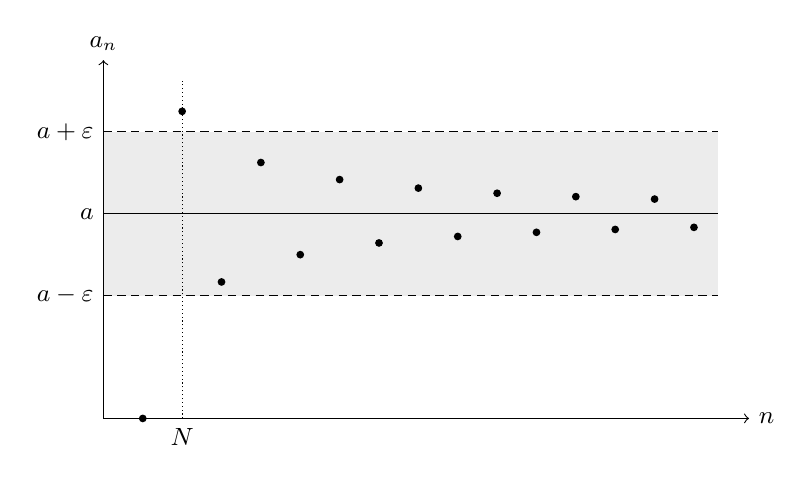
\begin{tikzpicture}[x=0.5cm,y=2.6cm,font=\small]
\fill[gray!15] (0,0.6) rectangle (15.6,1.4);
\draw[densely dashed] (0,0.6)--(15.6,0.6);
\draw[densely dashed] (0,1.4)--(15.6,1.4);
\draw (0,1)--(15.6,1);
\draw[->] (0,0)--(16.4,0) node[right] {$n$};
\draw[->] (0,0)--(0,1.75) node[above] {$a_n$};
\draw[densely dotted] (2,0)--(2,1.65);
\node[below] at (2,0) {$N$};
\node[left] at (0,1.4) {$a+\varepsilon$};
\node[left] at (0,1) {$a$};
\node[left] at (0,0.6) {$a-\varepsilon$};
\foreach \n in {1,...,15}{
  \pgfmathsetmacro{\yy}{1+(1-2*mod(\n,2))/\n}
  \fill (\n,\yy) circle (1.4pt);
}
\end{tikzpicture}
\end{center}

若只在数轴上画出各项的值, $|a_n-a|<\varepsilon$ 表示 $a_n$ 落在邻域 $U(a,\varepsilon)$ 中. 所以 $a_n\to a$ 的意思是: 无论邻域 $U(a,\varepsilon)$ 多么小, 数列从某项起全部落在其中, 落在外面的至多是 $a_1,\ldots,a_N$ 这有限多项. 反过来, 若对每个 $\varepsilon>0$, 落在 $U(a,\varepsilon)$ 外面的项只有有限多个, 取 $N$ 为这些项中最大的下标 (没有这样的项时取 $N=0$), 定义中的条件就成立. 这里按位置计数, 相同的数值出现在不同位置时算作不同的项. 例如 $\{(-1)^n\}$ 落在 $U(1,1)$ 外面的数值只有 $-1$, 但取这个值的项有无穷多个, 所以它不收敛于 $1$.

由此可知, 若 $a_n\to a$, 则改变数列的有限多项以后, 所得的数列仍收敛于 $a$. 这是因为对任意 $\varepsilon>0$, 新数列落在 $U(a,\varepsilon)$ 外面的项至多是原来那有限多项再加上被改动的有限多项, 仍然只有有限多个. 发散数列改变有限多项以后仍然发散. 如果改动后的数列收敛, 那么把这些项改回原值, 由刚才的结论, 原数列也收敛, 与它发散矛盾. 去掉前面若干项也不改变极限, 即对固定的正整数 $k$, 若 $a_n\to a$, 则数列 $\{a_{n+k}\}$ 也收敛于 $a$. 事实上, 任给 $\varepsilon>0$, 取 $a_n\to a$ 的定义中与 $\varepsilon$ 对应的 $N$, 当 $n>N$ 时 $n+k>N$, 故 $|a_{n+k}-a|<\varepsilon$.

数列不收敛于 $a$, 就是定义中的条件不成立. 其中“当 $n>N$ 时, 总有”就是“对任意 $n>N$, 都有”, 所以条件中依次有“对任意 $\varepsilon>0$”“存在 $N$”“对任意 $n>N$”三处量词. 否定这个条件时, 把这三处的“对任意”与“存在”互换, 次序保持不变, 再把最后的不等式 $|a_n-a|<\varepsilon$ 换成 $|a_n-a|\ge\varepsilon$, 得到: 存在某个 $\varepsilon_0>0$, 使对每个 $N\in\mathbb N$, 都有某个 $n>N$ 满足 $|a_n-a|\ge\varepsilon_0$. 用符号写成
\[
\exists\,\varepsilon_0>0,\ \ \forall\,N\in\mathbb N,\ \ \exists\,n>N:\ \ |a_n-a|\ge\varepsilon_0,
\]
其中 $\forall$ 读作“对任意”, $\exists$ 读作“存在”. 这个否定形式是说, 有一个固定的误差限度 $\varepsilon_0$, 无论从哪一项往后看, 总还有项与 $a$ 的距离不小于 $\varepsilon_0$. 因此这样的项有无穷多个, 它们都落在邻域 $U(a,\varepsilon_0)$ 外面. 数列发散, 则是指对每个实数 $a$ 都有上述情况.
\begin{example}\label{ex:12-div}
证明数列 $\{(-1)^n\}$ 发散.
\end{example}
\par\indent\textbf{分析:} 要说明任何实数 $a$ 都不是极限. 对固定的 $a$, 按否定形式, 需要选定一个误差 $\varepsilon_0$, 再对每个 $N$ 找出 $n>N$, 使 $(-1)^n$ 与 $a$ 的距离不小于 $\varepsilon_0$. 数列在 $1$ 与 $-1$ 两个值之间交替, 这两个值相距 $2$, 一个数 $a$ 不可能与两者的距离都小于 $1$. 所以取 $\varepsilon_0=1$. 对每个 $N$, 第 $N$ 项以后既有等于 $1$ 的项, 也有等于 $-1$ 的项, 其中取值离 $a$ 较远的项就是所需的项.
\begin{cnproof}
任取实数 $a$. 由三角不等式,
\[
|1-a|+|a-(-1)|\ge|1-(-1)|=2,
\]
所以 $|1-a|$ 与 $|-1-a|$ 中至少有一个不小于 $1$ (否则两者之和小于 $2$). 取 $\varepsilon_0=1$. 对任意 $N\in\mathbb N$, 奇数下标 $2N+1$ 与偶数下标 $2N+2$ 都大于 $N$, 且 $(-1)^{2N+1}=-1$, $(-1)^{2N+2}=1$, 其中必有一项与 $a$ 的距离不小于 $\varepsilon_0$. 所以 $\{(-1)^n\}$ 不收敛于 $a$. 由 $a$ 的任意性, $\{(-1)^n\}$ 发散.
\end{cnproof}
\subsection{用定义证明极限}
用定义证明 $a_n\to a$, 要做的是对每个 $\varepsilon>0$ 找出 $N$. 寻找 $N$ 的过程写在草稿上, 一般分三步.

(1) 写出误差 $|a_n-a|$ 并化简.

(2) 从目标 $|a_n-a|<\varepsilon$ 出发倒推. 要使它成立, 只需某个更简单的不等式成立, 这样逐步得到一个形如 $n>t$ 的条件, 其中 $t$ 只依赖于 $\varepsilon$ 和题中给定的常数. 这里只需要 $n>t$ 是 $|a_n-a|<\varepsilon$ 的充分条件, 不要求反过来也成立, 所以每一步不必是等价变形.

(3) 取 $N=[t]$; 若 $t<0$, 一切 $n$ 都满足条件, 取 $N=0$. 由 1.1 节, 整数 $n>[t]$ 时 $n\ge[t]+1>t$, 所以取 $N=[t]$ 就够了, 不必取成 $[t]+1$.

正式证明则按定义的次序书写: 先任给 $\varepsilon$, 再写出 $N$, 最后由 $n>N$ 推出 $|a_n-a|<\varepsilon$.
\begin{example}\label{ex:2-1}
\textnormal{(教材例2.1)} 证明 $\displaystyle\lim_{n\to\infty}\frac{n+1}n=1$.
\end{example}
\par\indent\textbf{分析:} 误差为 $\displaystyle\left|\frac{n+1}n-1\right|=\frac1n$. 要使 $\displaystyle\frac1n<\varepsilon$, 只需 $\displaystyle n>\frac1\varepsilon$, 所以取 $\displaystyle N=\left[\frac1\varepsilon\right]$; $\varepsilon>1$ 时 $N=0$, 这时所有项都符合要求.
\begin{cnproof}
任给 $\varepsilon>0$, 取 $\displaystyle N=\left[\frac1\varepsilon\right]$. 当 $n>N$ 时 $\displaystyle n>\frac1\varepsilon$, 于是
\[
\left|\frac{n+1}n-1\right|=\frac1n<\varepsilon.
\]
故 $\displaystyle\lim_{n\to\infty}\frac{n+1}n=1$.
\end{cnproof}
\begin{example}\label{ex:2-2}
\textnormal{(教材例2.2)} 设 $a>0$, 证明 $\displaystyle\lim_{n\to\infty}\frac1{n^a}=0$.
\end{example}
\par\indent\textbf{分析:} 误差为 $\displaystyle\frac1{n^a}$. 不等式 $\displaystyle\frac1{n^a}<\varepsilon$ 即 $\displaystyle n^a>\frac1\varepsilon$. 因为 $a>0$, 幂函数 $t^{\frac1a}$ 在 $(0,+\infty)$ 上严格增加, 两边同取 $\displaystyle\frac1a$ 次幂时不等号方向不变, 得到等价的条件 $n>\varepsilon^{-\frac1a}$. 所以取 $N=\bigl[\varepsilon^{-\frac1a}\bigr]$.
\begin{cnproof}
任给 $\varepsilon>0$, 取 $N=\bigl[\varepsilon^{-\frac1a}\bigr]$. 当 $n>N$ 时 $n>\varepsilon^{-\frac1a}$, 从而 $\displaystyle n^a>\frac1\varepsilon$, 即
\[
\left|\frac1{n^a}-0\right|=\frac1{n^a}<\varepsilon.
\]
故 $\displaystyle\lim_{n\to\infty}\frac1{n^a}=0$.
\end{cnproof}
条件 $a>0$ 在求解时用于保证幂函数递增, 它不能去掉. 若 $a\le0$, 则 $\displaystyle\frac1{n^a}=n^{-a}\ge1$, 所有项与 $0$ 的距离都不小于 $1$, 取 $\varepsilon_0=1$ 即知数列不收敛于 $0$.

以上两例的误差不等式都能直接解出 $n$. 下例中的两个数列, 误差不等式一个无法直接求解, 一个直接求解很繁, 需要另想办法.
\begin{example}\label{ex:h12-2}
\textnormal{(选自教材习题1.2第2题)} 证明 $\displaystyle\lim_{n\to\infty}\frac{\cos n}n=0$, $\displaystyle\lim_{n\to\infty}\bigl(\sqrt{n+1}-\sqrt n\bigr)=0$.
\end{example}
\par\indent\textbf{分析:} 第一个数列的误差是 $\displaystyle\frac{|\cos n|}n$. 分子 $|\cos n|$ 随 $n$ 不规则地变化, 不等式 $\displaystyle\frac{|\cos n|}n<\varepsilon$ 无法解出. 但只需要它成立的一个充分条件. 由 $|\cos n|\le1$,
\[
\left|\frac{\cos n}n-0\right|=\frac{|\cos n|}n\le\frac1n,
\]
所以只需 $\displaystyle\frac1n<\varepsilon$, 即 $\displaystyle n>\frac1\varepsilon$. 把误差换成较大而容易求解的量, 这种做法称为\textbf{放大}. 放大后的量必须仍能任意小. 若把误差放大成常数 $1$, 当 $\varepsilon\le1$ 时就得不到误差小于 $\varepsilon$.

第二个数列是两个无限增大的数之差, 从这个形式看不出差有多小; 直接解不等式 $\sqrt{n+1}-\sqrt n<\varepsilon$ 又要平方两次, 比较繁. 把误差分子有理化, 差就化成了分母无限增大的分式:
\[
\sqrt{n+1}-\sqrt n=\frac{(\sqrt{n+1}-\sqrt n)(\sqrt{n+1}+\sqrt n)}{\sqrt{n+1}+\sqrt n}=\frac1{\sqrt{n+1}+\sqrt n}<\frac1{2\sqrt n}.
\]
最后一步把分母中的 $\sqrt{n+1}$ 换成较小的 $\sqrt n$, 分式变大, 形式也更简单. 要使 $\displaystyle\frac1{2\sqrt n}<\varepsilon$, 只需 $\displaystyle\sqrt n>\frac1{2\varepsilon}$, 即 $\displaystyle n>\frac1{4\varepsilon^2}$.
\begin{cnproof}
任给 $\varepsilon>0$, 取 $\displaystyle N=\left[\frac1\varepsilon\right]$. 当 $n>N$ 时 $\displaystyle n>\frac1\varepsilon$, 所以
\[
\left|\frac{\cos n}n-0\right|=\frac{|\cos n|}n\le\frac1n<\varepsilon.
\]
故 $\displaystyle\lim_{n\to\infty}\frac{\cos n}n=0$.

对第二个数列, 任给 $\varepsilon>0$, 取 $\displaystyle N=\left[\frac1{4\varepsilon^2}\right]$. 当 $n>N$ 时 $\displaystyle n>\frac1{4\varepsilon^2}$, 即 $\displaystyle\sqrt n>\frac1{2\varepsilon}$, 所以
\[
\bigl|\sqrt{n+1}-\sqrt n-0\bigr|=\frac1{\sqrt{n+1}+\sqrt n}<\frac1{2\sqrt n}<\varepsilon.
\]
故 $\displaystyle\lim_{n\to\infty}\bigl(\sqrt{n+1}-\sqrt n\bigr)=0$.
\end{cnproof}
\begin{example}\label{ex:h12-4}
\textnormal{(选自教材习题1.2第4题)} 设 $|q|<1$, 证明 $\displaystyle\lim_{n\to\infty}q^n=0$.
\end{example}
\par\indent\textbf{分析:} 误差是 $|q^n-0|=|q|^n$. $n$ 出现在指数上, 解不等式 $|q|^n<\varepsilon$ 要取对数; $e$ 和自然对数到 1.4 节才定义, 这里用常用对数. $q=0$ 时 $\lg|q|$ 无意义, 但各项都是 $0$, 可以单独说明; 下面设 $0<|q|<1$. 由于 $\lg x$ 严格增加, 而 $\lg|q|<0$,
\[
|q|^n<\varepsilon\iff n\lg|q|<\lg\varepsilon\iff n>\frac{\lg\varepsilon}{\lg|q|},
\]
第二步两边除以负数 $\lg|q|$, 不等号反向. 当 $0<\varepsilon<1$ 时右端是正数, 取 $\displaystyle N=\left[\frac{\lg\varepsilon}{\lg|q|}\right]$; 当 $\varepsilon\ge1$ 时一切项都满足 $|q|^n<1\le\varepsilon$, 取 $N=0$.
\begin{cnproof}
若 $q=0$, 各项都是 $0$, 对任意 $\varepsilon>0$ 取 $N=0$ 即可. 下设 $0<|q|<1$, 并任给 $\varepsilon>0$.

若 $\varepsilon\ge1$, 取 $N=0$, 则一切 $n$ 都满足 $|q^n-0|=|q|^n<1\le\varepsilon$.

若 $0<\varepsilon<1$, 取 $\displaystyle N=\left[\frac{\lg\varepsilon}{\lg|q|}\right]$. 当 $n>N$ 时 $\displaystyle n>\frac{\lg\varepsilon}{\lg|q|}$, 两边乘以负数 $\lg|q|$ 得 $n\lg|q|<\lg\varepsilon$, 即 $\lg|q|^n<\lg\varepsilon$, 所以 $|q^n-0|=|q|^n<\varepsilon$.

故 $\displaystyle\lim_{n\to\infty}q^n=0$.
\end{cnproof}
本题也可以不用对数. 设 $0<|q|<1$. 要说明 $|q|^n$ 能任意小, 只需说明它的倒数 $\displaystyle\left(\frac1{|q|}\right)^n$ 能任意大. 这个乘幂的底数大于 $1$, 记 $\displaystyle\frac1{|q|}=1+c$, $c>0$, 就可以用二项式定理估计 $(1+c)^n$. 展开后各项都非负, 只保留前两项得 $(1+c)^n\ge1+nc>nc$, 于是 $\displaystyle|q|^n=\frac1{(1+c)^n}<\frac1{nc}$. 要使 $\displaystyle\frac1{nc}<\varepsilon$, 只需 $\displaystyle n>\frac1{c\varepsilon}$, 取 $\displaystyle N=\left[\frac1{c\varepsilon}\right]$ 即可, 不必区分 $\varepsilon$ 的大小.


\begin{example}\label{ex:2-3}
\textnormal{(教材例2.3)} 设 $\displaystyle\lim_{n\to\infty}a_n=a$, 证明
\[
\lim_{n\to\infty}\frac{a_1+a_2+\cdots+a_n}n=a.
\]
\end{example}
\par\indent\textbf{分析:} 要证明 $n$ 充分大时平均值与 $a$ 的距离小于 $\varepsilon$, 而已知条件控制的是各项与 $a$ 的距离 $|a_k-a|$, 所以先用各个 $a_k-a$ 表示平均值与 $a$ 的差. 把 $a$ 看作 $n$ 个 $a$ 的平均值, 两个平均值相减, 得
\[
\frac{a_1+\cdots+a_n}n-a=\frac{(a_1-a)+\cdots+(a_n-a)}n,
\]
对分子中的 $n$ 个数逐次使用三角不等式,
\[
\left|\frac{a_1+\cdots+a_n}n-a\right|\le\frac{|a_1-a|+\cdots+|a_n-a|}n.
\]
于是问题归结为估计各项误差 $|a_k-a|$ 的平均值. 由 $a_n\to a$, 对任意正数 $\eta$, 下标充分大以后 $|a_k-a|<\eta$. 但平均值包含从第一项起的全部 $n$ 项, 而收敛条件对前面的项没有任何限制, 它们的误差可能很大. 所以不能对所有项统一估计, 应当把和式分成两段: 前面误差不受控制的有限多项, 以及后面误差小于 $\eta$ 的项.

取定正数 $\eta$ 及相应的分界下标 $m$, 使 $k>m$ 时 $|a_k-a|<\eta$. 当 $n>m$ 时, 把各项误差的平均值按下标是否超过 $m$ 分成两段:
\[
\frac{|a_1-a|+\cdots+|a_m-a|}n+\frac{|a_{m+1}-a|+\cdots+|a_n-a|}n.
\]
后一段有 $n-m$ 项, 每项小于 $\eta$, 所以这一段小于 $\displaystyle\frac{(n-m)\eta}n\le\eta$; 项数虽然随 $n$ 增加, 但分母 $n$ 也同步增加. 前一段的分子 $C=|a_1-a|+\cdots+|a_m-a|$ 在 $m$ 取定以后是一个固定的数, 它可能很大, 但除以 $n$ 以后, 只要 $n$ 充分大就能任意小.

两段之和要小于 $\varepsilon$, 就让每段各小于 $\displaystyle\frac\varepsilon2$. 于是各量的选取次序是: 给定 $\varepsilon$ 后, 先取 $\displaystyle\eta=\frac\varepsilon2$, 由此确定 $m$; $m$ 确定后 $C$ 随之确定; 最后要求 $n$ 足够大, 使 $\displaystyle\frac Cn<\frac\varepsilon2$. 这个次序不能颠倒, 因为 $C$ 依赖于 $m$. 对 $n$ 的要求有 $n>m$ 和 $\displaystyle n>\frac{2C}\varepsilon$ 两条. 取 $N$ 为 $m$ 与 $\displaystyle\left[\frac{2C}\varepsilon\right]$ 中的较大者, 两条要求便同时满足.
\begin{cnproof}
任给 $\varepsilon>0$. 由 $a_n\to a$, 存在 $m\in\mathbb N$, 使 $k>m$ 时 $\displaystyle|a_k-a|<\frac\varepsilon2$. 令
\[
C=|a_1-a|+\cdots+|a_m-a|\quad(m=0\text{ 时 }C=0),\qquad N=\max\left\{m,\left[\frac{2C}\varepsilon\right]\right\}.
\]
当 $n>N$ 时, 有 $n>m$ 及 $\displaystyle n>\frac{2C}\varepsilon$, 即 $\displaystyle\frac Cn<\frac\varepsilon2$, 于是 (逐次使用三角不等式)
\[
\begin{aligned}
\left|\frac{a_1+\cdots+a_n}n-a\right|
&=\left|\frac{(a_1-a)+\cdots+(a_n-a)}n\right|\\
&\le\frac Cn+\frac{|a_{m+1}-a|+\cdots+|a_n-a|}n\\
&<\frac Cn+\frac{n-m}n\cdot\frac\varepsilon2
<\frac\varepsilon2+\frac\varepsilon2=\varepsilon.
\end{aligned}
\]
故 $\displaystyle\lim_{n\to\infty}\frac{a_1+a_2+\cdots+a_n}n=a$.
\end{cnproof}
反过来, 平均值收敛时 $\{a_n\}$ 不一定收敛. 例如 $a_n=(-1)^n$ 发散 (例\ref{ex:12-div}), 但它的前 $n$ 项之和为 $-1$ 或 $0$, 平均值的绝对值不超过 $\displaystyle\frac1n$. 由定义 (取 $\displaystyle N=\left[\frac1\varepsilon\right]$), 平均值趋于 $0$.
\begin{example}\label{ex:2-4}
\textnormal{(教材例2.4)} 证明 $\displaystyle\lim_{n\to\infty}\sqrt[n]n=1$.
\end{example}
\par\indent\textbf{分析:} 由 $n\ge1$ 知 $\sqrt[n]n\ge1$, 误差就是 $\sqrt[n]n-1$. 不等式 $\sqrt[n]n-1<\varepsilon$ 等价于 $n<(1+\varepsilon)^n$, 其中 $n$ 既出现在左边, 又出现在右边的指数上, 无法解出. 于是不去解 $n$, 改为直接估计误差的大小. 记 $h_n=\sqrt[n]n-1\ge0$, 则
\[
n=(1+h_n)^n.
\]
右边可以用二项式定理展开, 各项都非负, 保留其中一部分就得到一个关于 $h_n$ 的不等式, 从中可以解出 $h_n$ 的上界.

保留哪些项, 要看所得的上界是否趋于零. 只保留常数项和一次项, 得 $n\ge1+nh_n$, 即 $\displaystyle h_n\le\frac{n-1}n<1$. 这个上界不随 $n$ 变小, 不能用. 原因是一次项的系数 $n$ 与左边的 $n$ 大小相当, 约去以后只能得到 $h_n$ 有界. 二次项 $\displaystyle\frac{n(n-1)}2h_n^2$ 的系数比左边的 $n$ 大得多, 由它不超过 $n$ 就能得到趋于零的上界. 当 $n\ge2$ 时展开式中有这一项,
\[
n\ge\frac{n(n-1)}2h_n^2,
\]
两边除以正数 $\displaystyle\frac{n(n-1)}2$, 得 $\displaystyle h_n^2\le\frac2{n-1}$. 要使 $h_n<\varepsilon$, 只需 $h_n^2<\varepsilon^2$, 为此只需 $\displaystyle\frac2{n-1}<\varepsilon^2$, 即 $\displaystyle n>1+\frac2{\varepsilon^2}$. 这个条件同时保证了 $n\ge2$.
\begin{cnproof}
任给 $\varepsilon>0$, 取 $\displaystyle N=\left[1+\frac2{\varepsilon^2}\right]$. 当 $n>N$ 时 $\displaystyle n>1+\frac2{\varepsilon^2}$, 特别地 $n\ge2$. 令 $h_n=\sqrt[n]n-1\ge0$, 由二项式定理,
\[
n=(1+h_n)^n=1+nh_n+\frac{n(n-1)}2h_n^2+\cdots+h_n^n\ge\frac{n(n-1)}2h_n^2,
\]
所以
\[
h_n^2\le\frac2{n-1}<\varepsilon^2,
\]
从而 $\bigl|\sqrt[n]n-1\bigr|=h_n<\varepsilon$. 故 $\displaystyle\lim_{n\to\infty}\sqrt[n]n=1$.
\end{cnproof}
\par\indent\textbf{方法小结:} 用定义证明数列极限时, 寻找 $N$ 有三种情形. 误差不等式能直接解出 $n$ 时直接求解, 如例\ref{ex:2-1}、例\ref{ex:2-2}、例\ref{ex:h12-4}. 不便直接求解时先放大, 常用的办法有: 用 $|\cos n|\le1$ 一类的估计去掉有界因子, 根式之差先同乘共轭式再缩小分母 (例\ref{ex:h12-2}); 把大于 $1$ 的量写成 $1+h$, 在二项式展开中保留一部分项 (例\ref{ex:2-4}, 以及例\ref{ex:h12-4} 后面的说明). 放大后的量必须仍能任意小. 已知条件是另一个极限时, 由已知极限的定义取分界下标, 必要时把误差分成两段分别控制 (例\ref{ex:2-3}). 无论哪种情形, $N$ 只能依赖于 $\varepsilon$ 和题中给定的量, 不能依赖于 $n$.
\subsection{定义的等价形式与直接推论}
\begin{example}
\textnormal{(选自教材习题1.2第1题)} 在数列极限的定义中, 把“$n>N$”改为“$n\ge N$”, 或者把“$|a_n-a|<\varepsilon$”改为“$|a_n-a|\le\varepsilon$”, 收敛的概念是否改变?
\end{example}
\begin{cnsolution}
都不改变. 只需说明修改后的条件与原定义可以互相推出.

先看下标条件. 若原定义成立, 对给定的 $\varepsilon$ 有 $N$ 使 $n>N$ 时 $|a_n-a|<\varepsilon$; 令 $N'=N+1$, 则 $n\ge N'$ 时 $n>N$, 修改后的条件成立. 反过来, 若 $n\ge N'$ 时 $|a_n-a|<\varepsilon$, 则 $n>N'$ 时更是如此, 原定义成立.

再看误差条件. 由 $|a_n-a|<\varepsilon$ 自然得到 $|a_n-a|\le\varepsilon$. 反过来, 设对每个正数 $\eta$ 都有分界下标, 使以后的项满足 $|a_n-a|\le\eta$. 任给 $\varepsilon>0$, 把这个条件用于 $\displaystyle\eta=\frac\varepsilon2$, 得到 $N$, 使 $n>N$ 时
\[
|a_n-a|\le\frac\varepsilon2<\varepsilon,
\]
原定义成立. 由于误差可以任意给定, 对较小的误差使用非严格不等式, 就能得到原来误差下的严格不等式.
\end{cnsolution}
同样的道理表明, 定义中的误差限度 $\varepsilon$ 可以换成 $K\varepsilon$, 这里 $K>0$ 是与 $\varepsilon$、$n$ 都无关的常数. 也就是说, 若对任意 $\varepsilon>0$ 都能找到 $N$, 使 $n>N$ 时 $|a_n-a|<K\varepsilon$, 则 $a_n\to a$. 事实上, 对给定的 $\varepsilon$, 把这个条件用于 $\displaystyle\frac\varepsilon K$, 得到的 $N$ 使 $n>N$ 时 $\displaystyle|a_n-a|<K\cdot\frac\varepsilon K=\varepsilon$. 也可以只对 $\displaystyle\varepsilon=\frac1k$ ($k\in\mathbb N^+$) 验证, 因为任给 $\varepsilon>0$, 由阿基米德性质可取正整数 $\displaystyle k>\frac1\varepsilon$, 与 $\displaystyle\frac1k$ 对应的 $N$ 使 $n>N$ 时 $\displaystyle|a_n-a|<\frac1k<\varepsilon$. 但只对大于某个正数的 $\varepsilon$ 验证是不够的. 例如 $(-1)^n$ 与 $0$ 的距离对每个 $\varepsilon>1$ 都小于 $\varepsilon$, 它却不收敛于 $0$.
\begin{example}
\textnormal{(选自教材习题1.2第5、6题)} 证明: (1) 若 $a_n\to a$, 则 $|a_n|\to|a|$; (2) 若 $\{u_n\}$ 有界, $v_n\to0$, 则 $u_nv_n\to0$.
\end{example}
\par\indent\textbf{分析:} (1) 的误差是 $\bigl||a_n|-|a|\bigr|$, 已知条件能控制的是 $|a_n-a|$. 反三角不等式说明前者不超过后者, 所以原来的 $N$ 直接可用.

(2) 的误差是 $|u_nv_n|=|u_n|\,|v_n|$. $\{u_n\}$ 未必收敛, 但有界条件给出一个对所有下标都有效的常数 $M$, 使 $|u_n|\le M$, 于是误差不超过 $M|v_n|$. 只要预先让 $|v_n|$ 小于 $\displaystyle\frac\varepsilon M$, 误差就小于 $\varepsilon$. 这里 $M$ 在 $\varepsilon$ 给定之前就已确定, 用它来确定 $N$ 是允许的.
\begin{cnproof}
(1) 任给 $\varepsilon>0$. 由 $a_n\to a$, 存在 $N$, 使 $n>N$ 时 $|a_n-a|<\varepsilon$. 对这些 $n$, 由反三角不等式,
\[
\bigl||a_n|-|a|\bigr|\le|a_n-a|<\varepsilon.
\]
故 $|a_n|\to|a|$.

(2) 由 $\{u_n\}$ 有界, 存在 $M>0$, 使一切 $n$ 都满足 $|u_n|\le M$. 任给 $\varepsilon>0$. 由 $v_n\to0$, 对正数 $\displaystyle\frac\varepsilon M$, 存在 $N$, 使 $n>N$ 时 $\displaystyle|v_n|<\frac\varepsilon M$. 于是 $n>N$ 时
\[
|u_nv_n-0|=|u_n|\,|v_n|\le M|v_n|<\varepsilon.
\]
故 $u_nv_n\to0$.
\end{cnproof}
(1) 的逆命题不成立. 取 $a_n=(-1)^n$, 则 $\{|a_n|\}$ 的各项都是 $1$, 它收敛, 而 $\{a_n\}$ 发散. 但当 $a=0$ 时逆命题成立, 因为 $|a_n-0|$ 与 $\bigl||a_n|-0\bigr|$ 是同一个数.

(2) 不要求 $\{u_n\}$ 收敛. 例如 $\{(-1)^n\}$ 发散 (本节例\ref{ex:12-div}), 由 $\displaystyle\frac1n\to0$ 及 (2) 仍得 $\displaystyle\frac{(-1)^n}n\to0$. 本节例\ref{ex:h12-2} 的第一个结论也是 (2) 的特例, 那里只用到了 $|\cos n|\le1$.
\section{收敛数列的性质和运算}
用定义证明极限, 每遇到一个数列都要重新选取分界下标. 本节从定义出发证明收敛数列的几条一般性质, 并建立极限的四则运算法则. 有了这些结果, 许多数列的极限可以由已知的简单极限通过运算得到, 不必每次回到定义.
\subsection{唯一性、有界性与保序性}
\begin{theorem}[唯一性]
收敛数列的极限是唯一的.
\end{theorem}
设 $a_n\to a$ 且 $a_n\to b$, 要证 $a=b$. 从数轴上看, 若 $a\ne b$, 取 $\displaystyle\varepsilon=\frac{|a-b|}2$, 则邻域 $U(a,\varepsilon)$ 与 $U(b,\varepsilon)$ 不相交, 而 $a_n\to a$ 与 $a_n\to b$ 要求数列从某项起同时落在这两个邻域中, 这不可能. 已知条件只涉及 $a_n$ 与 $a$、$a_n$ 与 $b$ 的距离, 所以写成不等式时, 借助一项 $a_n$ 作中间的数, 由三角不等式得 $|a-b|\le|a-a_n|+|a_n-b|$. 当 $n$ 充分大时右边两项都小于 $\varepsilon$, 于是 $|a-b|<2\varepsilon=|a-b|$, 矛盾.
\begin{cnproof}
设 $a_n\to a$, $a_n\to b$. 若 $a\ne b$, 取 $\displaystyle\varepsilon=\frac{|a-b|}2>0$. 存在 $N_1,N_2$, 使 $n>N_1$ 时 $|a_n-a|<\varepsilon$, $n>N_2$ 时 $|a_n-b|<\varepsilon$. 取一个下标 $n>\max\{N_1,N_2\}$, 则
\[
|a-b|\le|a-a_n|+|a_n-b|<2\varepsilon=|a-b|,
\]
矛盾. 故 $a=b$.
\end{cnproof}
\begin{theorem}[有界性]
收敛数列必有界.
\end{theorem}
有界只要求全部项落在一个固定的范围内, 并不要求范围任意小, 所以在收敛定义中取一个确定的误差, 例如 $\varepsilon=1$, 就够了. 定义只控制分界以后的项, 分界以前的项可能很大, 但它们只有有限个, 用其中最大的绝对值作它们的界即可. 两部分的界中较大的一个, 就是全部项的界.
\begin{cnproof}
设 $a_n\to a$. 对 $\varepsilon=1$, 存在 $N\in\mathbb N$, 使 $n>N$ 时 $|a_n-a|<1$, 从而
\[
|a_n|\le|a_n-a|+|a|<|a|+1.
\]
令 $M=\max\{|a_1|,\ldots,|a_N|,|a|+1\}$ (当 $N=0$ 时 $M=|a|+1$), 则 $M>0$, 且 $n\le N$ 与 $n>N$ 时都有 $|a_n|\le M$.
\end{cnproof}
有界只是收敛的必要条件. 1.2 节例\ref{ex:12-div} 已经证明 $\{(-1)^n\}$ 发散, 它却是有界的. 定理的逆否命题是“无界数列必发散”, 常用来判断发散. 例如 $\{n\}$ 与 $\{(-1)^nn\}$ 都无界, 所以都发散.
\begin{theorem}[保序性]
设 $a_n\to a$, $b_n\to b$. \textup{(1)} 若 $a>b$, 则存在 $N$, 使 $n>N$ 时 $a_n>b_n$. \textup{(2)} 若存在 $N_0$, 使 $n>N_0$ 时 $a_n\ge b_n$, 则 $a\ge b$.
\end{theorem}
结论 (1) 中 $a>b$, 两个极限之间有正的间隔 $a-b$, 中点 $\displaystyle\frac{a+b}2$ 把它们隔开. 只要 $a_n$ 与 $a$ 的距离、$b_n$ 与 $b$ 的距离都小于间隔的一半, $a_n$ 就在中点右侧, $b_n$ 就在中点左侧, 于是 $a_n>b_n$. 结论 (2) 可以由 (1) 用反证法得到.
\begin{cnproof}
(1) 取 $\displaystyle\varepsilon=\frac{a-b}2>0$. 存在 $N_1,N_2$, 使 $n>N_1$ 时 $|a_n-a|<\varepsilon$, $n>N_2$ 时 $|b_n-b|<\varepsilon$. 取 $N=\max\{N_1,N_2\}$, 则 $n>N$ 时
\[
a_n>a-\varepsilon=\frac{a+b}2=b+\varepsilon>b_n.
\]

(2) 若 $a<b$, 交换两个数列的位置再用 (1), 存在 $N$, 使 $n>N$ 时 $a_n<b_n$. 取 $n>\max\{N,N_0\}$, 便与 $a_n\ge b_n$ 矛盾. 故 $a\ge b$.
\end{cnproof}
结论 (2) 中即使把条件加强为 $a_n>b_n$, 也只能得到 $a\ge b$, 因为取极限后严格不等号可能变成等号. 例如 $\displaystyle\frac1n>0$ 对一切 $n$ 成立, 而 $\displaystyle\lim_{n\to\infty}\frac1n=0$.

在保序性中取 $\{b_n\}$ 为常数列 $c$, 得到常用的特例: 若 $a>c$, 则从某项起 $a_n>c$; 若从某项起 $a_n\ge c$, 则 $a\ge c$. 取 $\{a_n\}$ 为常数列 $c$, 又得到不等号反向的特例: 若 $b<c$, 则从某项起 $b_n<c$; 若从某项起 $b_n\le c$, 则 $b\le c$.
\begin{corollarysingle}[保号性]
若 $a_n\to a$ 且 $a\ne0$, 则存在 $N$, 使 $n>N$ 时 $a_n$ 与 $a$ 同号, 并且 $\displaystyle|a_n|>\frac{|a|}2$.
\end{corollarysingle}
\begin{cnproof}
对 $\displaystyle\varepsilon=\frac{|a|}2>0$, 存在 $N$, 使 $n>N$ 时 $\displaystyle|a_n-a|<\frac{|a|}2$. 由反三角不等式,
\[
|a_n|\ge|a|-|a_n-a|>\frac{|a|}2.
\]
又当 $a>0$ 时 $\displaystyle a_n>a-\frac a2>0$, 当 $a<0$ 时 $\displaystyle a_n<a+\frac{|a|}2=\frac a2<0$.
\end{cnproof}
推论中的条件 $a\ne0$ 不能去掉. 极限为 $0$ 时, 数列的项可以不断变号, 例如 $\displaystyle\frac{(-1)^n}n\to0$. 推论的第二个结论说明, 极限不为零的数列从某项起不仅不等于零, 而且与零的距离大于固定的正数 $\displaystyle\frac{|a|}2$. 这一点在下面证明商的运算法则时要用到.
\subsection{四则运算法则}
\begin{theorem}[四则运算法则]
设 $a_n\to a$, $b_n\to b$. 则
\[
\lim_{n\to\infty}(a_n\pm b_n)=a\pm b,\qquad \lim_{n\to\infty}a_nb_n=ab;
\]
特别地, 对常数 $c$ 有 $\displaystyle\lim_{n\to\infty}ca_n=ca$. 若还有 $b\ne0$, 则 $b_n$ 从某项起不为零, 并且
\[
\lim_{n\to\infty}\frac{a_n}{b_n}=\frac ab.
\]
\end{theorem}
商数列只在 $b_n\ne0$ 的项上有定义. 当 $b\ne0$ 时, $b_n$ 从某项起不为零; 由 1.2 节, 去掉这一项以前的有限多项不影响极限, 所以只需考虑从这一项起的各项.

\par\indent\textbf{分析:} 已知条件能把 $|a_n-a|$ 与 $|b_n-b|$ 变得任意小. 证明每条结论, 都要把目标误差用这两个量估计出来.

和的误差是 $|(a_n+b_n)-(a+b)|=|(a_n-a)+(b_n-b)|$, 由三角不等式, 它不超过 $|a_n-a|+|b_n-b|$, 让两项各小于 $\displaystyle\frac\varepsilon2$ 即可. 差的情形相同.

积的误差 $a_nb_n-ab$ 中看不出 $a_n-a$ 与 $b_n-b$. 从 $a_nb_n$ 变到 $ab$, 两个因子都要换; 一次只换一个, 先把 $b_n$ 换成 $b$, 得到中间量 $a_nb$. 在误差中减去再加上 $a_nb$, 得
\[
a_nb_n-ab=(a_nb_n-a_nb)+(a_nb-ab)=a_n(b_n-b)+b(a_n-a),
\]
两项都是一个已知的小量乘以一个因子. 因子 $b$ 是常数; 因子 $a_n$ 随 $n$ 变化, 但由有界性, 它的绝对值不超过一个固定的数. 用同一个常数 $M$ 同时控制 $|a_n|$ 与 $|b|$, 误差就不超过 $M\bigl(|b_n-b|+|a_n-a|\bigr)$; 要使它小于 $\varepsilon$, 只需 $|a_n-a|$ 与 $|b_n-b|$ 都小于 $\displaystyle\frac\varepsilon{2M}$. 常数倍是积的特例, 只需把 $\{b_n\}$ 取为常数列 $c$.

商可以写成 $\displaystyle a_n\cdot\frac1{b_n}$, 有了积的法则, 只需证明 $\displaystyle\frac1{b_n}\to\frac1b$. 误差为
\[
\left|\frac1{b_n}-\frac1b\right|=\frac{|b_n-b|}{|b_n|\,|b|}.
\]
分子是已知的小量, 问题在分母. 若 $b_n$ 可以任意接近 $0$, 分式就可能很大. 但由 $b\ne0$ 及保号性推论, 从某项起 $\displaystyle|b_n|>\frac{|b|}2$, 即 $\displaystyle\frac1{|b_n|}<\frac2{|b|}$, 这时
\[
\frac{|b_n-b|}{|b_n|\,|b|}\le\frac2{|b|}\cdot\frac{|b_n-b|}{|b|}=\frac2{|b|^2}|b_n-b|,
\]
误差不超过 $|b_n-b|$ 的常数倍; 要使它小于 $\varepsilon$, 只需 $\displaystyle|b_n-b|<\frac{|b|^2\varepsilon}2$.
\begin{cnproof}
任给 $\varepsilon>0$.

和与差: 存在 $N_1,N_2$, 使 $n>N_1$ 时 $\displaystyle|a_n-a|<\frac\varepsilon2$, $n>N_2$ 时 $\displaystyle|b_n-b|<\frac\varepsilon2$. 当 $n>\max\{N_1,N_2\}$ 时,
\[
|(a_n\pm b_n)-(a\pm b)|\le|a_n-a|+|b_n-b|<\varepsilon.
\]

积: 由有界性, 存在 $M>0$, 使一切 $n$ 都有 $|a_n|\le M$; 必要时把 $M$ 换成 $\max\{M,|b|\}$, 可设还有 $|b|\le M$. 存在 $N_1,N_2$, 使 $n>N_1$ 时 $\displaystyle|a_n-a|<\frac\varepsilon{2M}$, $n>N_2$ 时 $\displaystyle|b_n-b|<\frac\varepsilon{2M}$. 当 $n>\max\{N_1,N_2\}$ 时,
\[
|a_nb_n-ab|=|a_n(b_n-b)+b(a_n-a)|\le M|b_n-b|+M|a_n-a|<\varepsilon.
\]

倒数: 设 $b\ne0$. 由保号性推论, 存在 $N_0$, 使 $n>N_0$ 时 $\displaystyle|b_n|>\frac{|b|}2>0$; 又存在 $N_1$, 使 $n>N_1$ 时 $\displaystyle|b_n-b|<\frac{|b|^2\varepsilon}2$. 当 $n>\max\{N_0,N_1\}$ 时,
\[
\left|\frac1{b_n}-\frac1b\right|=\frac{|b_n-b|}{|b_n|\,|b|}\le\frac2{|b|^2}|b_n-b|<\varepsilon.
\]
所以 $\displaystyle\frac1{b_n}\to\frac1b$. 由积的法则, $\displaystyle\frac{a_n}{b_n}=a_n\cdot\frac1{b_n}\to a\cdot\frac1b=\frac ab$.
\end{cnproof}
使用法则时要注意两点. 第一, 参与运算的每个数列都必须已知收敛, 商的情形还要求分母的极限不为零. 若 $\{a_n\}$, $\{b_n\}$ 都发散, 它们的和既可能收敛, 也可能发散. 例如 $(-1)^n$ 与 $(-1)^{n+1}$ 之和恒为 $0$, $(-1)^n$ 与自身之和则发散. 第二, 法则对固定个数的数列成立, 反复使用可以处理有限次运算, 但不能用于项数随 $n$ 增加的和. 例如对每个固定的 $k$ 都有 $\displaystyle\frac k{n^2}\to0$, 但
\[
\frac1{n^2}+\frac2{n^2}+\cdots+\frac n{n^2}=\frac{n(n+1)}{2n^2}=\frac{n+1}{2n}\to\frac12,
\]
而不是 $0$.
\begin{example}
\textnormal{(教材例3.1)} 求 $\displaystyle\lim_{n\to\infty}\frac{3n^3+n+1}{2n^3-5}$.
\end{example}
\par\indent\textbf{分析:} 分子、分母都无限增大, 都不收敛, 不能直接用商的法则. 它们的增长主要来自三次项, 所以分子、分母同除以 $n^3$. 这样分子变为 $\displaystyle3+\frac1{n^2}+\frac1{n^3}$, 分母变为 $\displaystyle2-\frac5{n^3}$, 都有极限, 并且分母的极限 $2$ 不为零, 就可以用商的法则了.
\begin{cnsolution}
由 1.2 节例\ref{ex:2-2} 的结论 $\displaystyle\frac1{n^a}\to0$ ($a>0$) 及四则运算法则,
\[
\begin{aligned}
\lim_{n\to\infty}\frac{3n^3+n+1}{2n^3-5}
&=\lim_{n\to\infty}\frac{3+\frac1{n^2}+\frac1{n^3}}{2-\frac5{n^3}}\\
&=\frac{\displaystyle\lim_{n\to\infty}\left(3+\frac1{n^2}+\frac1{n^3}\right)}{\displaystyle\lim_{n\to\infty}\left(2-\frac5{n^3}\right)}
=\frac{3+0+0}{2-0}=\frac32.
\end{aligned}
\]
\end{cnsolution}
一般地, 分子、分母都是 $n$ 的多项式时, 同除以分母的最高次幂 $n^k$. 分母随之趋于它的最高次项系数; 分子的次数等于 $k$ 时趋于它的最高次项系数, 次数小于 $k$ 时趋于 $0$, 大于 $k$ 时无界. 所以次数相同时极限是两个最高次项系数之比, 分子次数较低时极限是 $0$, 较高时数列无界, 因而发散.
\begin{example}
\textnormal{(教材例3.2)} 求 $\displaystyle\lim_{n\to\infty}\frac{1^2+2^2+\cdots+n^2}{n^3}$.
\end{example}
\par\indent\textbf{分析:} 分子的项数随 $n$ 增加, 而运算法则只适用于固定个数的数列, 所以不能逐项除以 $n^3$ 再相加取极限. 应先用平方和公式把分子写成 $n$ 的多项式, 化成两个多项式之比.
\begin{cnsolution}
由平方和公式
\[
1^2+2^2+\cdots+n^2=\frac{n(n+1)(2n+1)}6,
\]
得
\[
\lim_{n\to\infty}\frac{1^2+2^2+\cdots+n^2}{n^3}
=\lim_{n\to\infty}\frac{n(n+1)(2n+1)}{6n^3}
=\lim_{n\to\infty}\frac16\left(1+\frac1n\right)\left(2+\frac1n\right)
=\frac16\cdot1\cdot2=\frac13.
\]
\end{cnsolution}
平方和公式可以这样得到. 把恒等式 $(k+1)^3-k^3=3k^2+3k+1$ 对 $k=1,2,\ldots,n$ 相加, 左边依次相消, 只剩 $(n+1)^3-1$; 右边是 $3(1^2+\cdots+n^2)+3(1+\cdots+n)+n$. 代入 $\displaystyle1+2+\cdots+n=\frac{n(n+1)}2$, 得
\[
\begin{aligned}
3(1^2+\cdots+n^2)&=(n+1)^3-(n+1)-\frac{3n(n+1)}2\\
&=n(n+1)(n+2)-\frac{3n(n+1)}2=\frac{n(n+1)(2n+1)}2.
\end{aligned}
\]
\subsection{性质与运算法则的应用}
\begin{example}
\textnormal{(选自教材习题1.3第1题)} 设 $a_n\ge0$, $a_n\to a$, 用定义证明 $\sqrt{a_n}\to\sqrt a$.
\end{example}
\par\indent\textbf{分析:} 四则运算法则不包括开方, 因此开平方后的极限要回到定义来证明. 由保序性 $a\ge0$, 所以 $\sqrt a$ 有意义. 目标误差是 $|\sqrt{a_n}-\sqrt a|$, 已知能控制的是 $|a_n-a|$, 两者由平方差联系起来. 先设 $a>0$, 这时 $\sqrt{a_n}+\sqrt a\ge\sqrt a>0$, 乘以共轭式, 得
\[
|\sqrt{a_n}-\sqrt a|=\frac{|a_n-a|}{\sqrt{a_n}+\sqrt a}\le\frac{|a_n-a|}{\sqrt a}.
\]
分母随 $n$ 变化, 但有固定的正下界 $\sqrt a$, 所以目标误差不超过 $|a_n-a|$ 的常数倍; 要使它小于 $\varepsilon$, 只需 $|a_n-a|<\sqrt a\,\varepsilon$. 当 $a=0$ 时分母 $\sqrt{a_n}$ 没有正的下界, 还可能为零, 不能这样估计; 但这时目标 $\sqrt{a_n}<\varepsilon$ 就是 $a_n<\varepsilon^2$, 可以直接由收敛定义得到.
\begin{cnproof}
由 $a_n\ge0$ 及保序性, $a\ge0$. 任给 $\varepsilon>0$.

若 $a>0$, 存在 $N$, 使 $n>N$ 时 $|a_n-a|<\sqrt a\,\varepsilon$, 于是
\[
|\sqrt{a_n}-\sqrt a|=\frac{|a_n-a|}{\sqrt{a_n}+\sqrt a}\le\frac{|a_n-a|}{\sqrt a}<\varepsilon.
\]

若 $a=0$, 存在 $N$, 使 $n>N$ 时 $|a_n-0|<\varepsilon^2$, 即 $a_n<\varepsilon^2$, 从而 $|\sqrt{a_n}-0|=\sqrt{a_n}<\varepsilon$.

两种情形下都有 $\sqrt{a_n}\to\sqrt a$.
\end{cnproof}
\begin{example}
\textnormal{(选自教材习题1.3第4题)} 已知 $y_n-x_n\to0$, $x_n\to a$, 证明 $y_n\to a$.
\end{example}
\begin{cnproof}
已知收敛的是 $\{y_n-x_n\}$ 与 $\{x_n\}$, 待证的 $y_n$ 恰好是它们的和:
\[
y_n=(y_n-x_n)+x_n.
\]
由和的法则, $y_n\to0+a=a$.
\end{cnproof}
不能先写 $\displaystyle\lim_{n\to\infty}(y_n-x_n)=\lim_{n\to\infty}y_n-\lim_{n\to\infty}x_n$ 再移项, 因为差的法则要求 $\{y_n\}$ 已知收敛, 而这是待证的结论.
\section{数列收敛的判别定理}
用定义证明收敛, 必须先知道极限是多少. 许多数列的极限事先看不出来, 例如 $\displaystyle\left(1+\frac1n\right)^n$, 或者由递推式给出的数列; 有的数列即使知道极限, 误差不等式也解不出 $n$. 本节建立几个判别收敛的定理. 两边夹定理借助极限已知的数列来求极限, 不必解误差不等式; 单调收敛定理和柯西准则只根据数列自身的性质判断收敛, 不需要预先知道极限值. 除两边夹定理外, 这些定理都以确界原理为基础.
\subsection{两边夹定理}
\begin{theorem}[两边夹定理]
设存在 $N_0\in\mathbb N$, 使 $n>N_0$ 时 $a_n\le b_n\le c_n$, 并且 $a_n\to l$, $c_n\to l$. 则 $b_n\to l$.
\end{theorem}
条件没有直接给出 $b_n$ 与 $l$ 的距离. 不过 $a_n$ 与 $c_n$ 从某项起都落在邻域 $U(l,\varepsilon)$ 中, 而 $b_n$ 夹在它们之间, 于是 $l-\varepsilon<a_n\le b_n\le c_n<l+\varepsilon$, 即 $b_n$ 也落在这个邻域中.
\begin{cnproof}
任给 $\varepsilon>0$. 存在 $N_1$, 使 $n>N_1$ 时 $|a_n-l|<\varepsilon$, 从而 $a_n>l-\varepsilon$; 存在 $N_2$, 使 $n>N_2$ 时 $|c_n-l|<\varepsilon$, 从而 $c_n<l+\varepsilon$. 取 $N=\max\{N_0,N_1,N_2\}$, 当 $n>N$ 时
\[
l-\varepsilon<a_n\le b_n\le c_n<l+\varepsilon,
\]
即 $|b_n-l|<\varepsilon$. 故 $b_n\to l$.
\end{cnproof}
两端的数列必须趋于同一个数, 否则定理不能给出结论. 例如 $-1\le(-1)^n\le1$, 两端的极限不同, 而 $\{(-1)^n\}$ 发散.

使用这个定理, 要为所给的数列找到上下两个容易求极限、并且极限相同的数列. 误差不等式解不出 $n$ 时, 常用的是定理的一个特殊情形. 若从某项起 $|b_n-l|\le c_n$, 且 $c_n\to0$, 把定理用于 $0\le|b_n-l|\le c_n$, 就得到 $|b_n-l|\to0$, 按定义这就是 $b_n\to l$. 这样只需把 $|b_n-l|$ 放大成一个容易求极限的 $c_n$, 不必再解关于 $n$ 的不等式. 放大的办法与 1.2 节相同, 同样要求放大后的 $c_n$ 仍趋于 $0$.
\begin{example}\label{ex:4-1}
\textnormal{(教材例4.1)} 设 $a>0$, 证明 $\displaystyle\lim_{n\to\infty}\frac{a^n}{n!}=0$.
\end{example}
\par\indent\textbf{分析:} $a>1$ 时分子和分母都无限增大, 要说明的是分母增长得更快. 不等式 $\displaystyle\frac{a^n}{n!}<\varepsilon$ 中 $n$ 同时出现在乘幂和阶乘里, 解不出 $n$, 所以用两边夹定理. 各项都是正数, 下界可以取 $0$, 只需再找一个趋于零的上界. 把通项写成 $n$ 个因子的乘积
\[
\frac{a^n}{n!}=\frac a1\cdot\frac a2\cdot\cdots\cdot\frac an,
\]
就可以逐个考察因子. 取定正整数 $k>a$, 当 $j>k$ 时 $\displaystyle\frac aj<1$. 若把这些因子全部放大成 $1$, 得到的上界是常数 $\displaystyle\frac{a^k}{k!}$, 不趋于零, 放得过大; 所以要保留一个趋于零的因子, 最简单的是最后一个因子 $\displaystyle\frac an$. 当 $n>k$ 时把因子分成三组:
\[
\frac{a^n}{n!}=\left(\frac a1\cdot\frac a2\cdot\cdots\cdot\frac ak\right)\cdot\left(\frac a{k+1}\cdot\cdots\cdot\frac a{n-1}\right)\cdot\frac an.
\]
第一组之积是与 $n$ 无关的常数 $\displaystyle\frac{a^k}{k!}$; 第二组的每个因子都在 $0$ 与 $1$ 之间, 乘积不超过 $1$; 第三组趋于零. 由此得到上界 $\displaystyle\frac{a^k}{k!}\cdot\frac an$, 它是常数乘 $\displaystyle\frac1n$.
\begin{cnproof}
取定正整数 $k>a$. 当 $n>k$ 时, 因子 $\displaystyle\frac a{k+1},\ldots,\frac a{n-1}$ 都在 $0$ 与 $1$ 之间 ($n=k+1$ 时没有这些因子), 所以
\[
0<\frac{a^n}{n!}=\frac{a^k}{k!}\cdot\frac a{k+1}\cdots\frac a{n-1}\cdot\frac an\le\frac{a^k}{k!}\cdot\frac an=\frac{a^{k+1}}{k!}\cdot\frac1n.
\]
$\displaystyle\frac{a^{k+1}}{k!}$ 与 $n$ 无关, 由 $\displaystyle\frac1n\to0$ 及常数倍法则, 右端趋于 $0$. 由两边夹定理, $\displaystyle\frac{a^n}{n!}\to0$.
\end{cnproof}
对任意实数 $a$, 由 $\displaystyle\left|\frac{a^n}{n!}\right|=\frac{|a|^n}{n!}$ 知同样有 $\displaystyle\frac{a^n}{n!}\to0$ ($a=0$ 时各项为 $0$).
\begin{example}\label{ex:4-2}
\textnormal{(教材例4.2)} 设 $a>0$, 证明 $\displaystyle\lim_{n\to\infty}\sqrt[n]a=1$.
\end{example}
\par\indent\textbf{分析:} 先看 $a>1$ 的情形, 这时 $\sqrt[n]a>1$. 与 1.2 节例\ref{ex:2-4} 一样, 把误差记为 $h_n=\sqrt[n]a-1>0$, 则 $a=(1+h_n)^n$, 由二项式定理, $a\ge1+nh_n$, 即
\[
0<h_n\le\frac{a-1}n.
\]
这里只保留一次项就够了. 在 1.2 节例\ref{ex:2-4} 中, 等式是 $n=(1+h_n)^n$, 只保留一次项得到 $n\ge1+nh_n$, 由此只能推出 $h_n<1$; 现在等式左边是固定的 $a$, 由 $nh_n\le a-1$ 就得到趋于零的上界. 至于 $0<a<1$ 的情形, 这时 $h_n<0$, 展开式各项正负相间, 不能随意舍去其中的项, 所以取倒数化为 $\displaystyle\frac1a>1$.
\begin{cnproof}
$a=1$ 时各项为 $1$. 设 $a>1$, 令 $h_n=\sqrt[n]a-1$, 则 $h_n>0$. 由二项式定理, $a=(1+h_n)^n\ge1+nh_n$, 故
\[
0<\sqrt[n]a-1\le\frac{a-1}n.
\]
右端趋于 $0$, 由两边夹定理, $\sqrt[n]a-1\to0$, 即 $\sqrt[n]a\to1$.

设 $0<a<1$, 则 $\displaystyle\frac1a>1$, 由已证情形 $\displaystyle\sqrt[n]{\frac1a}\to1$. 由商的法则,
\[
\lim_{n\to\infty}\sqrt[n]a=\lim_{n\to\infty}\frac1{\sqrt[n]{\frac1a}}=\frac1{\displaystyle\lim_{n\to\infty}\sqrt[n]{\frac1a}}=1.
\]
\end{cnproof}
$a>1$ 时也可以利用 1.2 节例\ref{ex:2-4} 的结论 $\sqrt[n]n\to1$. 当 $n>a$ 时 $1<\sqrt[n]a<\sqrt[n]n$, 再用两边夹定理.
\subsection{单调收敛定理}
\begin{definition}
若对每个 $n\in\mathbb N^+$ 都有 $a_n\le a_{n+1}$, 则称数列 $\{a_n\}$ \textbf{单调增加}; 若对每个 $n$ 都有 $a_n\ge a_{n+1}$, 则称 $\{a_n\}$ \textbf{单调减少}. 不等号都为严格时, 分别称为\textbf{严格单调增加}与\textbf{严格单调减少}. 单调增加和单调减少的数列统称\textbf{单调数列}.
\end{definition}
单调性和有界性单独都不能保证收敛. 例如 $\{n\}$ 单调增加但无界, $\{(-1)^n\}$ 有界但不单调, 两者都发散. 两个条件合在一起时, 数列一定收敛.
\begin{theorem}[单调收敛定理]
单调增加且有上界的数列收敛, 其极限是各项组成的数集的上确界; 单调减少且有下界的数列收敛, 其极限是各项组成的数集的下确界.
\end{theorem}
\par\indent\textbf{分析:} 用定义证明收敛要先有极限值, 这里的极限值只能从数列本身找出来. 单调增加的数列逐项上升, 又不超过上界, 它应当逼近所有上界中最小的那个, 即上确界 $s$; 确界原理保证 $s$ 存在. 要证明 $n$ 充分大时 $s-\varepsilon<a_n<s+\varepsilon$. 右边的不等式对每一项都成立, 因为 $s$ 是上界. 左边的不等式要求充分靠后的每一项都大于 $s-\varepsilon$, 而确界的刻画只保证有一项 $a_{n_0}>s-\varepsilon$. 由单调性, 这一项后面的各项都不小于它, 因而也都大于 $s-\varepsilon$, 所以 $N$ 可以取 $n_0$.
\begin{cnproof}
设 $\{a_n\}$ 单调增加且有上界. 由确界原理, 数集 $\{a_n:n\in\mathbb N^+\}$ 有上确界, 记为 $s$. 任给 $\varepsilon>0$, 由确界的刻画, 存在 $n_0$, 使 $a_{n_0}>s-\varepsilon$. 取 $N=n_0$, 当 $n>N$ 时, 由单调性和 $s$ 是上界,
\[
s-\varepsilon<a_{n_0}\le a_n\le s,
\]
所以 $|a_n-s|<\varepsilon$, 即 $a_n\to s$.

若 $\{a_n\}$ 单调减少且有下界, 则 $\{-a_n\}$ 单调增加且有上界. 由已证部分及 1.1 节确界的推论,
\[
-a_n\to\sup\{-a_n:n\in\mathbb N^+\}=-\inf\{a_n:n\in\mathbb N^+\},
\]
再由常数倍法则, $a_n\to\inf\{a_n:n\in\mathbb N^+\}$.
\end{cnproof}
由于改变有限多项不影响收敛性, 数列从某项起单调并且有界时同样收敛. 由定理的逆否命题还可以知道, 单调增加而发散的数列一定没有上界. 定理指出极限是上确界或下确界, 但确界的数值一般并不知道, 所以这个定理通常只用来判断极限存在.
\begin{example}\label{ex:4-3}
\textnormal{(教材例4.3)} 证明数列 $\displaystyle a_n=\left(1+\frac1n\right)^n$ 收敛.
\end{example}
\par\indent\textbf{分析:} 前几项约为 $2$, $2.25$, $2.37$, $2.44$, 逐项增大而增幅变小. 极限值事先看不出来, 所以考虑用单调收敛定理, 这需要证明数列单调, 并找出与 $n$ 无关的上界. 直接比较 $a_n$ 与 $a_{n+1}$ 有困难, 因为 $n$ 增大时底数 $\displaystyle1+\frac1n$ 变小, 指数却变大, 两种变化的影响方向相反. 用二项式定理把乘幂展开成和, 就可以逐项比较. 展开式中含 $\displaystyle\frac1{n^k}$ 的一项记为 $T_k(n)$, 它是
\[
\frac{n(n-1)\cdots(n-k+1)}{k!}\cdot\frac1{n^k}=\frac1{k!}\left(1-\frac1n\right)\left(1-\frac2n\right)\cdots\left(1-\frac{k-1}n\right),
\]
这是把分子的 $k$ 个因子分别除以 $n$ 得到的. 在这个形式中, 每个括号都是正数, 并且随 $n$ 增大而增大, 所以 $T_k(n)$ 也随 $n$ 增大. 此外 $a_{n+1}$ 的展开式比 $a_n$ 多出一个正项, 于是 $a_{n+1}>a_n$. 另一方面, 每个括号都小于 $1$, 把它们都换成 $1$, 就得到上界 $\displaystyle2+\frac1{2!}+\cdots+\frac1{n!}$. 它仍随 $n$ 变化, 又不能直接求和, 所以再用 $k!\ge2^{k-1}$ 把它放大成等比数列的和.
\begin{cnproof}
记
\[
T_k(n)=\frac1{k!}\left(1-\frac1n\right)\left(1-\frac2n\right)\cdots\left(1-\frac{k-1}n\right)\qquad(2\le k\le n).
\]
由二项式定理, $a_1=2$, 当 $n\ge2$ 时
\[
a_n=\left(1+\frac1n\right)^n=1+1+T_2(n)+T_3(n)+\cdots+T_n(n).
\]
把 $n$ 换成 $n+1$, 得 $a_{n+1}=1+1+T_2(n+1)+\cdots+T_n(n+1)+T_{n+1}(n+1)$. 对同一个 $k$, $T_k(n)$ 与 $T_k(n+1)$ 都是 $\displaystyle\frac1{k!}$ 乘以 $k-1$ 个括号, 只是每个括号 $\displaystyle1-\frac jn$ 换成了较大的 $\displaystyle1-\frac j{n+1}$; 这些括号都是正数, 所以 $T_k(n+1)>T_k(n)$. 此外 $a_{n+1}$ 还多出一个正项 $T_{n+1}(n+1)$. 所以对一切 $n\in\mathbb N^+$ 都有 $a_{n+1}>a_n$ ($n=1$ 时只有多出的那一项), $\{a_n\}$ 严格单调增加.

每个括号都在 $0$ 与 $1$ 之间, 所以 $\displaystyle T_k(n)<\frac1{k!}$, 当 $n\ge2$ 时
\[
a_n<2+\frac1{2!}+\frac1{3!}+\cdots+\frac1{n!}.
\]
当 $k\ge2$ 时, $k!=1\cdot2\cdot3\cdots k$ 中后 $k-1$ 个因子都不小于 $2$, 故 $k!\ge2^{k-1}$. 于是
\[
a_n<2+\frac12+\frac1{2^2}+\cdots+\frac1{2^{n-1}}=2+1-\frac1{2^{n-1}}<3.
\]
又 $a_1=2<3$. 数列单调增加且有上界 $3$, 由单调收敛定理, 它收敛.
\end{cnproof}
\begin{definition}
数列 $\displaystyle\left(1+\frac1n\right)^n$ 的极限记为 $e$, 即
\[
e=\lim_{n\to\infty}\left(1+\frac1n\right)^n.
\]
以 $e$ 为底的对数称为\textbf{自然对数}, 记作 $\ln x$.
\end{definition}
由本节例\ref{ex:4-3} 及单调收敛定理, $e$ 是数集 $\{a_n:n\in\mathbb N^+\}$ 的上确界, 所以 $\displaystyle e\ge a_2=\frac94$; 又各项都小于 $3$, 由保序性 $e\le3$. 更精确地计算可得 $e\approx2.71828$. 1.6 节的第二个重要极限以及 1.8 节中指数函数和对数函数的极限, 都以这个定义为出发点.
\begin{example}\label{ex:4-4}
\textnormal{(教材例4.4)} 设 $a_1=4$, $\displaystyle a_{n+1}=\frac1{a_n}+\frac{a_n}2$ ($n\in\mathbb N^+$), 求 $\displaystyle\lim_{n\to\infty}a_n$.
\end{example}
\par\indent\textbf{分析:} 通项没有显式的表达式, 无法直接估计误差. 先看极限如果存在会是多少. 设 $a_n\to l$. 数列 $\{a_{n+1}\}$ 只是 $\{a_n\}$ 去掉第一项, 也有 $a_{n+1}\to l$; 若 $l\ne0$, 在递推式两边取极限, 得 $\displaystyle l=\frac1l+\frac l2$, 即 $l^2=2$. 各项都是正数, 所以候选值是 $\sqrt2$. 这一计算以极限存在为前提, 它只说明极限如果存在并且不为零, 就只能是 $\sqrt2$.

再证明极限存在. 前几项约为 $4$, $2.25$, $1.57$, $1.42$, 逐项减小, 并且都大于 $\sqrt2\approx1.414$, 所以尝试用单调收敛定理. 要证单调减少, 看相邻两项之差:
\[
a_{n+1}-a_n=\frac1{a_n}-\frac{a_n}2=\frac{2-a_n^2}{2a_n},
\]
它的符号取决于 $a_n$ 与 $\sqrt2$ 的大小. 所以先证明各项不小于 $\sqrt2$, 这同时也是单调收敛定理需要的下界. 把递推式写成 $\displaystyle a_{n+1}=\frac12\left(a_n+\frac2{a_n}\right)$, 就可以看出 $a_{n+1}$ 是两个正数 $a_n$ 与 $\displaystyle\frac2{a_n}$ 的算术平均值, 而它们的乘积为 $2$, 由中学的均值不等式即得 $a_{n+1}\ge\sqrt2$.
\begin{cnsolution}
由 $a_1>0$ 及递推式, 用归纳法知各项都是正数, 递推式中的除法始终有意义. 由均值不等式, 对每个 $n$,
\[
a_{n+1}=\frac12\left(a_n+\frac2{a_n}\right)\ge\sqrt{a_n\cdot\frac2{a_n}}=\sqrt2,
\]
所以 $n\ge2$ 时 $a_n\ge\sqrt2$; 又 $a_1=4>\sqrt2$, 故一切项都不小于 $\sqrt2$. 于是
\[
a_{n+1}-a_n=\frac1{a_n}-\frac{a_n}2=\frac{2-a_n^2}{2a_n}\le0,
\]
数列单调减少且有下界 $\sqrt2$. 由单调收敛定理, $\{a_n\}$ 收敛, 设其极限为 $l$; 由保序性, $l\ge\sqrt2>0$.

$\{a_{n+1}\}$ 也收敛于 $l$. 因 $l\ne0$, 在递推式两边取极限, 由四则运算法则得 $\displaystyle l=\frac1l+\frac l2$, 即 $l^2=2$. 又 $l>0$, 所以 $\displaystyle\lim_{n\to\infty}a_n=\sqrt2$.
\end{cnsolution}
如果没有先证明收敛, 由递推式解出的数值就没有根据. 例如 $b_1=1$, $b_{n+1}=-b_n$, 形式地取极限得 $l=-l$, 即 $l=0$, 但 $\{b_n\}$ 就是发散的数列 $\{(-1)^{n+1}\}$.
\subsection{闭区间套定理}
后面的致密性定理、有限覆盖定理以及 1.9 节连续函数的零点定理, 都用逐次二分区间的办法缩小范围, 再由下面的闭区间套定理确定所需的点.
\begin{theorem}[闭区间套定理]
设闭区间 $I_n=[a_n,b_n]$ ($n\in\mathbb N^+$) 满足 $I_{n+1}\subseteq I_n$, 并且 $b_n-a_n\to0$. 则存在唯一的实数 $l$ 属于所有的 $I_n$, 并且 $a_n\to l$, $b_n\to l$.
\end{theorem}
\par\indent\textbf{分析:} 公共点必须不小于每个左端点, 又不大于每个右端点. 区间一个套一个, 意味着左端点只能向右移动, 右端点只能向左移动, 而且任何一个左端点都不超过任何一个右端点. 于是两个端点数列都单调有界, 由单调收敛定理各有极限. 长度趋于零使两个极限相等, 这个共同的极限就是要找的点.
\begin{cnproof}
由 $I_{n+1}\subseteq I_n$ 得 $a_n\le a_{n+1}\le b_{n+1}\le b_n$, 所以 $\{a_n\}$ 单调增加, $\{b_n\}$ 单调减少; 又 $a_n\le b_n\le b_1$, $b_n\ge a_n\ge a_1$. 由单调收敛定理, 两个数列都收敛, 设 $a_n\to\alpha$, $b_n\to\beta$. 由差的法则, $\displaystyle\beta-\alpha=\lim_{n\to\infty}(b_n-a_n)=0$, 记 $l=\alpha=\beta$. 固定 $n$, 把 $a_n$, $b_n$ 看作常数. 对任意 $m\ge n$, 有 $a_n\le a_m$ 及 $b_m\le b_n$; 而当 $m\to\infty$ 时 $a_m\to l$, $b_m\to l$, 由保序性 (与常数比较) 得 $a_n\le l\le b_n$, 即 $l\in I_n$.

若 $h$ 也属于所有的 $I_n$, 则 $a_n\le h\le b_n$ 对一切 $n$ 成立. 由两边夹定理, 常数列 $h$ 的极限是 $l$, 即 $h=l$.
\end{cnproof}
定理的三个条件各有作用. 区间必须是闭的, 因为证明中取极限只得到非严格不等式 $a_n\le l\le b_n$, 只能保证 $l$ 落在闭区间中. 例如开区间 $\displaystyle\left(0,\frac1n\right)$ 一个套一个, 长度趋于零, 右端点趋于 $0$, 而 $0$ 恰好是被去掉的左端点, 所以这些区间没有公共点. 区间还必须一个套一个. 闭区间 $\displaystyle\left[n,n+\frac1n\right]$ 的长度也趋于零, 但 $I_2$ 与 $I_3$ 已经不相交, 没有公共点. 长度趋于零保证公共点唯一. 若每个 $I_n$ 都是 $[0,1]$, 公共点就有无穷多个.
\subsection{子列与致密性定理}
\begin{definition}
设 $n_1<n_2<\cdots<n_k<\cdots$ 是严格增加的正整数列. 数列 $a_{n_1},a_{n_2},\ldots,a_{n_k},\ldots$ 称为 $\{a_n\}$ 的\textbf{子数列}, 简称\textbf{子列}, 记作 $\{a_{n_k}\}$.
\end{definition}
子列中的项保持它们在原数列中的先后顺序. 取子列时可以跳过一些项, 但不能颠倒顺序, 也不能重复使用同一个位置. 例如 $a_1,a_3,a_5,\ldots$ 与 $a_2,a_4,a_6,\ldots$ 都是子列, 而 $a_2,a_1,a_4,a_3,\ldots$ 不是. 在 $\{a_{n_k}\}$ 中, $k$ 是该项在子列中的序号, $n_k$ 是它在原数列中的序号. 由 $n_1\ge1$ 及 $n_{k+1}\ge n_k+1$, 用归纳法得 $n_k\ge k$.
\begin{theorem}
若 $a_n\to a$, 则 $\{a_n\}$ 的每个子列都收敛于 $a$.
\end{theorem}
\begin{cnproof}
任给 $\varepsilon>0$, 取 $N$, 使 $n>N$ 时 $|a_n-a|<\varepsilon$. 当 $k>N$ 时 $n_k\ge k>N$, 所以 $|a_{n_k}-a|<\varepsilon$. 故 $a_{n_k}\to a$ ($k\to\infty$).
\end{cnproof}
反过来, 若每个子列都收敛于 $a$, 则原数列 (它是自己的子列) 也收敛于 $a$. 由这个定理, 若能找到两个极限不同的子列, 或者找到一个发散的子列, 原数列就发散. 但一个子列收敛不能说明原数列收敛.
\begin{example}\label{ex:14-sub}
\textnormal{(教材正文中的子列判别示例)} 说明数列 $\{(-1)^n\}$ 发散.
\end{example}
\begin{cnproof}
偶数项组成的子列恒为 $1$, 奇数项组成的子列恒为 $-1$, 两者的极限分别是 $1$ 与 $-1$. 若原数列收敛于 $a$, 则它的每个子列都收敛于 $a$, 于是 $1=a=-1$, 矛盾. 故 $\{(-1)^n\}$ 发散.
\end{cnproof}
1.2 节例\ref{ex:12-div} 用定义证明同一结论时, 要对每个候选的极限值寻找远离它的项; 借助子列, 只需比较两个子列的极限. 对正负交替的数列, 通常先看奇数项与偶数项两个子列.

有界数列不一定收敛, 例如本节例\ref{ex:14-sub} 中的 $\{(-1)^n\}$, 但它的偶数项和奇数项子列都收敛.
\begin{theorem}[致密性定理]
有界数列必有收敛子列.
\end{theorem}
\par\indent\textbf{分析:} 设数列的各项都在 $[-M,M]$ 中. 要选出收敛的子列, 先要找到子列的极限 $l$. 若子列收敛于 $l$, 则 $l$ 的任意小的邻域中都有数列的无穷多项, 所以要找的是具有这种性质的点. 这样的点事先不知道在哪里, 可以用逐次二分的办法来确定. 每次把区间二等分, 保留含有无穷多项的那一半, 最后由闭区间套定理得到 $l$. 然后从保留下来的各个区间中依次各选一项, 并使下标逐个增大, 就得到所需的子列. 保留的区间要含有无穷多项, 是因为选取时每一步都要找下标比上一步大的项; 区间中若只有有限多项, 选到某一步就可能找不到.
\begin{cnproof}
设 $M>0$, $|a_n|\le M$ 对一切 $n$ 成立. 令 $I_1=[-M,M]$, 它含有数列的全部项. 把 $I_1$ 二等分, 若两个半区间都只含有限多项, 则 $I_1$ 也只含有限多项, 矛盾; 所以至少有一个半区间含有无穷多项, 取它为 $I_2$. 对 $I_2$ 作同样的讨论得 $I_3$, 依此类推, 得到闭区间 $I_k=[u_k,v_k]$, 它们满足 $I_{k+1}\subseteq I_k$, 每个都含有数列的无穷多项, 并且
\[
0<v_k-u_k=\frac{2M}{2^{k-1}}\le\frac{2M}k,
\]
这里由二项式定理得 $2^{k-1}=(1+1)^{k-1}\ge1+(k-1)=k$, 所以 $v_k-u_k\to0$. 由闭区间套定理, 存在 $l$, 使 $u_k\to l$, $v_k\to l$.

取 $n_1=1$. 设已取定 $n_{k-1}$. $I_k$ 中含有无穷多项, 而下标不超过 $n_{k-1}$ 的项只有 $n_{k-1}$ 个, 所以其中必有下标大于 $n_{k-1}$ 的项, 取一个这样的下标作为 $n_k$. 这样得到 $n_1<n_2<\cdots$, 并且 $u_k\le a_{n_k}\le v_k$. 由两边夹定理, $a_{n_k}\to l$.
\end{cnproof}
这个定理也称为波尔查诺--魏尔斯特拉斯定理. 有界的条件不能去掉, 例如 $\{n\}$ 的任何子列都无界, 因而都发散.
\subsection{柯西收敛准则}
单调收敛定理只适用于单调数列. 对一般的数列, 也希望能不借助极限值判断收敛. 若 $a_n\to a$, 则充分靠后的项都接近 $a$, 因而彼此也接近. 柯西准则说明, 反过来, 充分靠后的项彼此接近, 也足以保证收敛.
\begin{definition}
若对任意 $\varepsilon>0$, 存在 $N\in\mathbb N$, 使任意 $m,n>N$ 都满足 $|a_m-a_n|<\varepsilon$, 则称 $\{a_n\}$ 为\textbf{柯西数列}, 也称\textbf{基本数列}.
\end{definition}
在 1.2 节的图中, 数列收敛于 $a$ 要求第 $N$ 项以后的点 $(n,a_n)$ 都落在以直线 $y=a$ 为中线、宽度为 $2\varepsilon$ 的水平带中. 柯西条件只要求这些点两两之间的高度差小于 $\varepsilon$. 拿其中的点 $(N+1,a_{N+1})$ 来比较, 就知道这些点都落在以直线 $y=a_{N+1}$ 为中线、宽度为 $2\varepsilon$ 的水平带中. 这条带的中线由数列自己的项确定, 所以柯西条件不涉及极限值.

条件中的 $m,n$ 是分界以后的任意两个下标, 它们可以相距很远. 只检验相邻两项是不够的, 本节例\ref{ex:4-6} 将说明, 相邻两项之差趋于零的数列也可能发散. 由于 $m,n$ 的地位对称, 不妨设 $m>n$, 记 $m=n+p$, 条件也可以写成: 任给 $\varepsilon>0$, 存在 $N$, 使 $n>N$ 时对一切正整数 $p$ 都有 $|a_{n+p}-a_n|<\varepsilon$. 这里的 $N$ 只依赖于 $\varepsilon$, 对所有的 $p$ 同时有效.
\begin{theorem}[柯西收敛准则]
数列收敛的充分必要条件是它为柯西数列.
\end{theorem}
\par\indent\textbf{分析:} 先看必要性. 若 $a_n\to a$, 则 $|a_m-a_n|\le|a_m-a|+|a-a_n|$, 右边两项都能任意小.

充分性的困难在于没有现成的极限值, 必须从数列本身找出一个. 单调收敛定理要求数列单调, 而柯西数列不一定单调, 所以改用致密性定理, 这个定理只要求数列有界. 柯西条件确实能推出有界. 事实上, 取 $\varepsilon=1$, 得到分界 $N_0$, 以后的项与固定的一项 $a_{N_0+1}$ 相距都小于 $1$. 于是数列有收敛子列 $a_{n_k}\to a$, $a$ 就是候选的极限值. 子列只控制被选中的项, 其余的项要靠柯西条件来控制. 对 $\displaystyle\frac\varepsilon2$ 取柯西条件的分界 $N$, 再在子列中取定一项 $a_{n_k}$, 使 $n_k>N$ 并且 $\displaystyle|a_{n_k}-a|<\frac\varepsilon2$, 则对每个 $n>N$,
\[
|a_n-a|\le|a_n-a_{n_k}|+|a_{n_k}-a|<\frac\varepsilon2+\frac\varepsilon2=\varepsilon.
\]
\begin{cnproof}
必要性. 设 $a_n\to a$. 任给 $\varepsilon>0$, 存在 $N$, 使 $n>N$ 时 $\displaystyle|a_n-a|<\frac\varepsilon2$. 当 $m,n>N$ 时,
\[
|a_m-a_n|\le|a_m-a|+|a-a_n|<\varepsilon.
\]

充分性. 设 $\{a_n\}$ 是柯西数列. 对 $\varepsilon=1$, 存在 $N_0$, 使 $m,n>N_0$ 时 $|a_m-a_n|<1$. 于是 $n>N_0$ 时
\[
|a_n|\le|a_n-a_{N_0+1}|+|a_{N_0+1}|<|a_{N_0+1}|+1.
\]
取 $M=\max\{|a_1|,\ldots,|a_{N_0}|,|a_{N_0+1}|+1\}$, 则一切 $n$ 都满足 $|a_n|\le M$. 由致密性定理, 有子列 $a_{n_k}\to a$.

任给 $\varepsilon>0$. 由柯西条件, 存在 $N$, 使 $m,n>N$ 时 $\displaystyle|a_m-a_n|<\frac\varepsilon2$. 由 $a_{n_k}\to a$, 存在 $K$, 使 $k>K$ 时 $\displaystyle|a_{n_k}-a|<\frac\varepsilon2$. 取定一个 $k>\max\{K,N\}$, 则 $n_k\ge k>N$. 于是对每个 $n>N$,
\[
|a_n-a|\le|a_n-a_{n_k}|+|a_{n_k}-a|<\frac\varepsilon2+\frac\varepsilon2=\varepsilon.
\]
故 $a_n\to a$.
\end{cnproof}
充分性的证明用到了致密性定理, 归根结底依赖确界原理. 有理数不满足确界原理, 在有理数范围内充分性也不成立, 即由有理数组成的柯西数列可以没有有理数极限. 例如 $\sqrt2$ 的不足近似值 $1,\ 1.4,\ 1.41,\ 1.414,\ldots$ 组成一个有理数列, 第 $n$ 项以后的各项与第 $n$ 项的前 $n-1$ 位小数都相同, 相差小于 $10^{1-n}$, 所以它是柯西数列; 它在实数中的极限 $\sqrt2$ 却不是有理数.
\begin{example}\label{ex:4-5}
\textnormal{(教材例4.5)} 设 $a$ 是实数, 证明数列
\[
s_n=1+a+\frac{a^2}{2!}+\cdots+\frac{a^n}{n!}
\]
收敛.
\end{example}
\par\indent\textbf{分析:} 极限值不知道; 当 $a<0$ 时各项交替地增减, 数列也不单调. 因此考虑柯西准则. 对 $n$ 和正整数 $p$,
\[
s_{n+p}-s_n=\frac{a^{n+1}}{(n+1)!}+\cdots+\frac{a^{n+p}}{(n+p)!},
\]
共 $p$ 项. 每一项都很小, 但 $p$ 可以任意大, 不能用“最大的一项乘以项数”来估计, 需要一个与 $p$ 无关的上界. 公比小于 $1$ 的正项等比数列, 无论取多少项, 和都不超过一个固定的数, 所以把这 $p$ 项与等比数列比较, 先看相邻两项之比. 记 $r=|a|$. 第 $j+1$ 项与第 $j$ 项的绝对值之比为 $\displaystyle\frac r{n+j+1}$, 当 $n+2>2r$ 时
\[
\frac r{n+j+1}\le\frac r{n+2}<\frac12\qquad(j\ge1).
\]
这时从第二项起, 每一项的绝对值不超过前一项的一半, $p$ 项的绝对值之和不超过首项的绝对值乘以 $\displaystyle1+\frac12+\cdots+\frac1{2^{p-1}}=2-\frac1{2^{p-1}}<2$. 所得的上界 $\displaystyle\frac{2r^{n+1}}{(n+1)!}$ 不含 $p$, 并且由本节例\ref{ex:4-1} 趋于零.
\begin{cnproof}
记 $r=|a|$. 若 $r=0$, 各项都是 $1$, 数列收敛. 下设 $r>0$. 对任意 $n$ 和正整数 $p$, 由三角不等式,
\[
|s_{n+p}-s_n|\le\frac{r^{n+1}}{(n+1)!}+\frac{r^{n+2}}{(n+2)!}+\cdots+\frac{r^{n+p}}{(n+p)!}.
\]
当 $n+2>2r$ 时, 对 $j=1,2,\ldots,p-1$ 有 $\displaystyle\frac r{n+j+1}\le\frac r{n+2}<\frac12$, 所以
\[
\frac{r^{n+j+1}}{(n+j+1)!}=\frac r{n+j+1}\cdot\frac{r^{n+j}}{(n+j)!}<\frac12\cdot\frac{r^{n+j}}{(n+j)!},
\]
逐次使用这一估计可知, 在 $|s_{n+p}-s_n|$ 的估计式中, 右端第 $j$ 项不超过第一项的 $\displaystyle\frac1{2^{j-1}}$, 从而
\[
|s_{n+p}-s_n|\le\frac{r^{n+1}}{(n+1)!}\left(1+\frac12+\cdots+\frac1{2^{p-1}}\right)<\frac{2r^{n+1}}{(n+1)!}.
\]
由本节例\ref{ex:4-1}, $\displaystyle\frac{r^n}{n!}\to0$; $\displaystyle\frac{2r^{n+1}}{(n+1)!}$ 是它去掉第一项后再乘以 $2$, 所以也趋于 $0$. 任给 $\varepsilon>0$, 存在 $N_1$, 使 $n>N_1$ 时 $\displaystyle\frac{2r^{n+1}}{(n+1)!}<\varepsilon$. 取 $N=\max\{[2r],N_1\}$, 则 $n>N$ 时 $n>2r$, 更有 $n+2>2r$, 于是对一切正整数 $p$ 都有 $|s_{n+p}-s_n|<\varepsilon$, 而 $N$ 与 $p$ 无关. 由柯西准则, $\{s_n\}$ 收敛.
\end{cnproof}
本题只证明了极限存在, 柯西准则不能给出极限值.
\begin{example}\label{ex:4-6}
\textnormal{(教材例4.6)} 证明数列 $\displaystyle H_n=1+\frac12+\cdots+\frac1n$ 发散, 并说明相邻两项之差趋于零不能保证数列收敛.
\end{example}
\par\indent\textbf{分析:} 相邻两项之差 $\displaystyle H_{n+1}-H_n=\frac1{n+1}$ 趋于零, 只比较相邻两项看不出发散. 柯西条件涉及任意两个尾项, 要否定它, 应找一个固定的 $\varepsilon_0$, 使在任意远处都有两项之差不小于 $\varepsilon_0$. 当 $m>n$ 时, $H_m-H_n$ 是从 $\displaystyle\frac1{n+1}$ 到 $\displaystyle\frac1m$ 的和, 每一项都很小, 但项数 $m-n$ 可以随 $n$ 一起增大. 这 $m-n$ 项都不小于 $\displaystyle\frac1m$, 所以和不小于 $\displaystyle\frac{m-n}m=1-\frac nm$. 让 $m$ 是 $n$ 的固定倍数, 例如 $m=2n$, 这个下界就是固定的 $\displaystyle\frac12$.
\begin{cnproof}
对任意正整数 $n$,
\[
H_{2n}-H_n=\frac1{n+1}+\frac1{n+2}+\cdots+\frac1{2n}\ge n\cdot\frac1{2n}=\frac12.
\]
取 $\displaystyle\varepsilon_0=\frac12$. 对任意 $N\in\mathbb N$, 取 $n=N+1$, 则 $n$ 与 $2n$ 都大于 $N$, 而 $|H_{2n}-H_n|\ge\varepsilon_0$. 所以 $\{H_n\}$ 不是柯西数列, 由柯西准则, 它发散. 又 $\{H_n\}$ 单调增加, 由单调收敛定理, 它没有上界.

另一方面, $\displaystyle H_{n+1}-H_n=\frac1{n+1}\to0$. 收敛数列的相邻两项之差一定趋于零, 本例说明反过来不成立.
\end{cnproof}
\begin{example}
\textnormal{(选自教材习题1.4第12题)} 若对每个固定的正整数 $p$, 都有 $\displaystyle\lim_{n\to\infty}|a_{n+p}-a_n|=0$, 能否推出 $\{a_n\}$ 是柯西数列?
\end{example}
\par\indent\textbf{分析:} 题设条件写开来是: 对每个 $p$ 和每个 $\varepsilon>0$, 存在 $N$, 使 $n>N$ 时 $|a_{n+p}-a_n|<\varepsilon$. 这里先给定 $p$ 再找 $N$, 所以 $N$ 可以随 $p$ 改变; 柯西条件则要求同一个 $N$ 对所有 $p$ 都有效. 两者只在量词的次序上不同. 要说明不能推出, 需要一个数列, 对每个固定的 $p$ 都有 $a_{n+p}-a_n\to0$, 而当 $p$ 随 $n$ 适当增大时, 例如取 $p=n$, 这个差不趋于零. 本节例\ref{ex:4-6} 中的 $\{H_n\}$ 就是这样的数列.
\begin{cnsolution}
不能. 取 $\displaystyle H_n=1+\frac12+\cdots+\frac1n$. 对每个固定的正整数 $p$, 差中的 $p$ 项都小于 $\displaystyle\frac1n$, 所以
\[
0<H_{n+p}-H_n=\frac1{n+1}+\cdots+\frac1{n+p}<\frac pn,
\]
由两边夹定理, $\displaystyle\lim_{n\to\infty}|H_{n+p}-H_n|=0$. 但由本节例\ref{ex:4-6}, $\{H_n\}$ 不是柯西数列. 由 $\displaystyle\frac pn<\varepsilon$ 得到的分界 $\displaystyle\frac p\varepsilon$ 随 $p$ 增大而增大; 对一切 $p$ 都有效的 $N$ 确实不存在, 因为取 $p=n$ 时总有 $\displaystyle H_{2n}-H_n\ge\frac12$.
\end{cnsolution}
\par\indent\textbf{方法小结:} 通项能由已知极限的数列经有限次四则运算得到时, 用运算法则. 通项不便化简, 但能夹在两个极限相同的数列之间时, 用两边夹定理; 找上下界的常用办法是把一部分因子或项换成较大、较小的简单量, 并保留起决定作用的部分 (例\ref{ex:4-1}、例\ref{ex:4-2}). 不知道极限, 但数列单调时, 用单调收敛定理, 这时所找的界必须与 $n$ 无关. 证明单调时先算几项看方向, 再作差定号 (例\ref{ex:4-4}), 或者展开后逐项比较 (例\ref{ex:4-3}). 由递推式给出的数列, 先假定极限存在, 由递推式求出候选值. 再证明各项都在候选值的同一侧, 这给出了界, 也定出了单调方向. 由单调收敛定理得到收敛以后, 才能在递推式两边取极限 (例\ref{ex:4-4}). 既不单调、又不知道极限时, 用柯西准则, 估计 $|a_{n+p}-a_n|$ 时要得到与 $p$ 无关的上界 (例\ref{ex:4-5}). 证明发散时, 可以找两个极限不同的子列 (例\ref{ex:14-sub}), 说明数列无界, 或者否定柯西条件 (例\ref{ex:4-6}).
\subsection{实数完备性的几种等价表述}
本节从确界原理出发, 依次证明了单调收敛定理、闭区间套定理、致密性定理和柯西准则, 每一个都由前一个推出. 这里的单调收敛定理只指“单调有界数列必收敛”, 不包括“极限是确界”, 因为确界的存在本身就要由确界原理保证. 在这些推导中, 只有第一步用到确界原理, 其余各步只用到前一个定理、阿基米德性质和极限的基本性质. 反过来, 这四个定理中的任何一个也能推出确界原理. 所以它们都可以作为实数完备性的表述, 选择哪一个作为公理, 只是出发点不同.

在有理数范围内这几个结论都不成立: 1.1 节中由小于 $\sqrt2$ 的正有理数组成的集合 $S$ 没有有理数上确界; $\sqrt2$ 的不足近似值组成的有理数列 $1,\ 1.4,\ 1.41,\ldots$ 单调增加、有上界, 它和它的子列都没有有理数极限; 闭区间 $[1,2],\ [1.4,1.5],\ [1.41,1.42],\ldots$ 一个套一个, 长度趋于零, 也没有有理数公共点. 这些例子缺少的都是 $\sqrt2$ 这一个点, 即 1.1 节所说的“空隙”.
\begin{theorem}[实数完备性的等价表述]
在实数的四则运算、大小顺序和阿基米德性质的基础上, 确界原理、单调收敛定理、闭区间套定理、致密性定理与柯西收敛准则彼此等价.
\end{theorem}
\begin{cnproof}
正向的推导前面已经完成, 并且除第一步外都没有用到确界原理. 其中闭区间套定理的证明由保序性得到 $a_n\le l\le b_n$, 没有用“极限是确界”; 致密性定理的证明中, 区间长度趋于零只用到 $2^{k-1}\ge k$ 和阿基米德性质.

下面由其余四个定理分别推出确界原理, 它们共用同一个构造. 上确界应当是“上界”与“非上界”的分界点. 构造中让每个区间的左端点都不是上界、右端点都是上界, 再逐次二分, 使区间收缩到一点, 这一点就是要找的上确界.

设 $A$ 是非空且有上界的实数集. 取 $x_0\in A$ 及 $A$ 的一个上界 $v_1$, 令 $u_1=x_0-1$, 则 $u_1$ 不是 $A$ 的上界, 且 $u_1<v_1$. 取 $[u_1,v_1]$ 的中点 $c$. 若 $c$ 是 $A$ 的上界, 令 $[u_2,v_2]=[u_1,c]$, 否则令 $[u_2,v_2]=[c,v_1]$. 对 $[u_2,v_2]$ 重复这一做法, 依此类推. 得到的区间满足 $[u_{n+1},v_{n+1}]\subseteq[u_n,v_n]$, 每个 $u_n$ 都不是上界, 每个 $v_n$ 都是上界, 并且
\[
v_n-u_n=\frac{v_1-u_1}{2^{n-1}}\le\frac{v_1-u_1}n,
\]
这里由二项式定理得 $2^{n-1}=(1+1)^{n-1}\ge1+(n-1)=n$. 由阿基米德性质, $v_n-u_n\to0$.

再说明 $u_n$ 与 $v_n$ 有共同的极限 $s$. 若用闭区间套定理, 这是它的直接结论. 若用单调收敛定理, $\{u_n\}$ 单调增加且以 $v_1$ 为上界, 故 $u_n\to s$, 再由 $v_n=u_n+(v_n-u_n)$ 得 $v_n\to s$. 若用柯西准则, 当 $m\ge n$ 时 $u_n\le u_m\le v_m\le v_n$, 于是 $0\le u_m-u_n\le v_n-u_n$; 由 $v_n-u_n\to0$ 知 $\{u_n\}$ 是柯西数列, 它收敛于某个 $s$, 同样 $v_n\to s$. 若用致密性定理, 有界的 $\{u_n\}$ 有子列 $u_{n_k}\to s$. 由于 $\{u_n\}$ 单调增加, 对每个固定的 $n$, 当 $n_k\ge n$ 时 $u_n\le u_{n_k}$, 令 $k\to\infty$ 得 $u_n\le s$. 任给 $\varepsilon>0$, 取定一个 $k$ 使 $s-u_{n_k}<\varepsilon$, 则 $n\ge n_k$ 时 $0\le s-u_n\le s-u_{n_k}<\varepsilon$, 所以 $u_n\to s$, 同样 $v_n\to s$.

最后证明 $s=\sup A$. 每个 $x\in A$ 都满足 $x\le v_n$, 由保序性 $x\le s$, 所以 $s$ 是上界. 任给 $\varepsilon>0$, 由 $u_n\to s$, 存在 $n$ 使 $u_n>s-\varepsilon$; $u_n$ 不是上界, 所以有 $x\in A$ 使 $x>u_n>s-\varepsilon$. 由确界的刻画, $s=\sup A$.
\end{cnproof}
\subsection{有限覆盖定理与聚点原理}
实数的完备性还可以用有限覆盖定理和聚点原理来表述.
\begin{definition}
设 $E\subseteq\mathbb R$. 若一族开区间的并集包含 $E$, 则称这族开区间为 $E$ 的一个\textbf{开覆盖}. 若能从中选出有限个开区间, 它们的并集仍包含 $E$, 则称这个开覆盖有\textbf{有限子覆盖}.
\end{definition}
直观地说, 开覆盖就是用一族开区间把 $E$ 盖住; 有限子覆盖就是从中只留下有限个开区间, 仍然盖住 $E$.

开覆盖不一定有有限子覆盖. 例如开区间 $\displaystyle\left(0,\frac n{n+1}\right)$ ($n\in\mathbb N^+$) 覆盖 $(0,1)$, 因为对任意 $x\in(0,1)$, 只要 $\displaystyle\frac1{n+1}<1-x$, 就有 $\displaystyle x<1-\frac1{n+1}=\frac n{n+1}$. 但任取其中有限个, 它们的右端点中最大的一个仍小于 $1$, 比它大的点就没有被盖住. 又如开区间 $(-1,n)$ ($n\in\mathbb N^+$) 覆盖 $[0,+\infty)$, 其中任意有限个都盖不住整个 $[0,+\infty)$. 这两个例子中, $(0,1)$ 不是闭区间, $[0,+\infty)$ 无界.
\begin{theorem}[有限覆盖定理]
闭区间 $[a,b]$ 的任意开覆盖都有有限子覆盖.
\end{theorem}
\par\indent\textbf{分析:} 开覆盖是任意给定的, 没有一般的办法直接构造有限子覆盖, 所以用反证法. 假设 $[a,b]$ 的某个开覆盖没有有限子覆盖. 用二分法可以找出一串闭区间, 每一个都不能被有限个开区间覆盖, 它们收缩到一点 $l$. 由于 $l\in[a,b]$, 覆盖中有一个开区间含有 $l$, 它也含有 $l$ 的某个邻域. 足够靠后的闭区间都落在这个邻域中, 只用这一个开区间就能盖住, 与它们不能被有限个开区间覆盖矛盾. 得出 $l\in[a,b]$ 要用到区间是闭的. 对上面 $(0,1)$ 的例子作同样的二分, 区间收缩到的点是 $1$, 它不属于 $(0,1)$, 覆盖中的开区间 $\displaystyle\left(0,\frac n{n+1}\right)$ 都不含有它, 也就推不出矛盾.
\begin{cnproof}
反设 $[a,b]$ 的某个开覆盖没有有限子覆盖. 把 $[a,b]$ 二等分, 若两个半区间都能被这个覆盖中的有限个开区间覆盖, 则 $[a,b]$ 也能, 矛盾; 所以至少有一个半区间不能被有限个覆盖, 记为 $I_1$. 对 $I_1$ 重复这一讨论, 依此类推, 得到闭区间 $I_n=[a_n,b_n]$, 满足 $I_{n+1}\subseteq I_n$, 每个 $I_n$ 都不能被有限个开区间覆盖, 并且 $\displaystyle b_n-a_n=\frac{b-a}{2^n}\to0$ (1.2 节例\ref{ex:h12-4}).

由闭区间套定理, 存在 $l$ 属于所有的 $I_n$, 且 $a_n\to l$, $b_n\to l$. 由于 $l\in[a,b]$, 覆盖中有某个开区间 $J$ 包含 $l$. 取 $r>0$, 使 $U(l,r)\subseteq J$. 若 $J=(\alpha,\beta)$, 取 $r=\min\{l-\alpha,\beta-l\}$, 即 $l$ 到 $J$ 两端距离中较小的一个; 若 $J$ 有一端无界, 只看另一端; 两端都无界时任取 $r>0$. 由 $a_n\to l$, $b_n\to l$, 当 $n$ 充分大时 $l-r<a_n$ 且 $b_n<l+r$, 即 $I_n\subseteq U(l,r)\subseteq J$. 这时单独一个开区间 $J$ 就覆盖了 $I_n$, 矛盾.
\end{cnproof}
在更一般的理论中, 具有有限覆盖性质的集合称为\textbf{紧集}, 实数轴上的闭区间是其中最基本的例子.
\begin{definition}
设 $E\subseteq\mathbb R$, $a\in\mathbb R$. 若 $a$ 的每一个邻域都含有 $E$ 的无穷多个点, 则称 $a$ 为 $E$ 的\textbf{聚点}.
\end{definition}
聚点可以属于 $E$, 也可以不属于 $E$. 例如 $0$ 是 $\displaystyle\left\{\frac1n:n\in\mathbb N^+\right\}$ 的聚点, 但不属于这个集合. 定义中的“点”指集合中互不相同的元素, 与数列按下标计数的“项”不同. 常数数列 $1,1,1,\ldots$ 有无穷多项, 它的各项组成的集合却只有一个元素, 因而没有聚点.

聚点也可以这样刻画: $a$ 的每一个去心邻域都含有 $E$ 中的点. 事实上, 若每个邻域含有无穷多个点, 去掉中心以后仍有点. 反过来的方向用逆否命题证明. 若某个邻域 $U(a,r)$ 只含 $E$ 的有限多个点, 取 $d$ 为其中异于 $a$ 的点到 $a$ 的最短距离 (没有这样的点时取 $d=r$), 则去心邻域 $\mathring U(a,d)$ 中没有 $E$ 的点.
\begin{theorem}[聚点原理]
有界的无限实数集至少有一个聚点.
\end{theorem}
\par\indent\textbf{分析:} $E$ 有界, 所以含于某个闭区间 $[a,b]$. 聚点的位置事先不知道, 因此用反证法. 若 $[a,b]$ 中每一点都不是聚点, 则每一点都有一个邻域, 其中只含 $E$ 的有限多个点. 由有限覆盖定理, 这些邻域中的有限个就能盖住 $[a,b]$; 有限个这样的邻域合起来只含 $E$ 的有限多个点, 与 $E$ 是无限集矛盾. 这里先在每一点附近得到局部的结论, 再用有限个邻域得到整体的结论, 这是有限覆盖定理的典型用法.
\begin{cnproof}
设 $E$ 有界且是无限集, 取闭区间 $[a,b]\supseteq E$. 反设 $[a,b]$ 中没有 $E$ 的聚点, 则对每个 $x\in[a,b]$, 都有一个邻域 $U_x$ 只含 $E$ 的有限多个点. 全体 $U_x$ 构成 $[a,b]$ 的开覆盖, 由有限覆盖定理, 其中有限个 $U_{x_1},\ldots,U_{x_m}$ 已覆盖 $[a,b]$, 从而覆盖 $E$. 每个 $U_{x_j}$ 只含 $E$ 的有限多个点, 所以 $E$ 只有有限多个点, 矛盾. 故 $E$ 在 $[a,b]$ 中有聚点.
\end{cnproof}
聚点原理的两个条件都不能去掉. 有限集没有聚点; $\mathbb N^+$ 是无限集, 但无界, 每个 $\displaystyle U\left(a,\frac12\right)$ 中至多有一个正整数, 所以它也没有聚点.

由聚点原理还能推出致密性定理, 从而推出确界原理. 设 $\{a_n\}$ 有界. 若某个数值出现无穷多次, 由这些项组成的常数子列就收敛. 否则每个数值只出现有限次, 而项有无穷多个, 所以各项组成的集合是有界无限集, 它有聚点 $l$; 在 $\displaystyle U\left(l,\frac1k\right)$ ($k=1,2,\ldots$) 中依次选取下标递增的项, 就得到趋于 $l$ 的子列. 于是由有限覆盖定理可以依次推出聚点原理、致密性定理和确界原理. 有限覆盖定理又是由闭区间套定理证明的, 因此有限覆盖定理和聚点原理也都与确界原理等价.
\section{函数的极限}
数列的下标只能无限增大, 函数的自变量则可以有多种变化方式: $x$ 可以趋于 $+\infty$ 或 $-\infty$, 也可以从两侧或一侧接近一个有限的点. 各种函数极限的定义都沿用数列极限的思想, 即对任意给定的误差, 找出自变量的一个范围, 使自变量在这个范围内时, 函数值都满足误差要求. 变化方式不同, 这个范围的写法就不同, 函数值的变化趋势也可能不同. 例如 $x\to-\infty$ 时 $2^x$ 无限接近 $0$, 而 $x\to+\infty$ 时 $2^x$ 无限增大. 所以极限记号中必须写明自变量的变化方式.
\subsection{自变量趋于无穷时的极限}
\begin{definition}
设函数 $f$ 在区间 $(c,+\infty)$ 内有定义, $L$ 是实数. 若对任意 $\varepsilon>0$, 都存在正数 $A$ ($A\ge c$), 使当 $x>A$ 时恒有
\[
|f(x)-L|<\varepsilon,
\]
则称当 $x\to+\infty$ 时 $f(x)$ 以 $L$ 为\textbf{极限}, 记作
\[
\lim_{x\to+\infty}f(x)=L\qquad\text{或}\qquad f(x)\to L\ (x\to+\infty).
\]
\end{definition}
这个定义与数列极限的定义类似, $\varepsilon$ 仍是任意给定的误差, 阈值 $A$ 代替了分界下标 $N$. 与 $N$ 一样, $A$ 可以随 $\varepsilon$ 改变, 但不能依赖于 $x$; 一个 $A$ 适用时, 更大的数也适用. 区别在于 $x$ 取遍 $(A,+\infty)$ 中的一切实数, 而不只是整数, 所以 $A$ 直接取为实数即可, 不需要取整. 条件 $A\ge c$ 只是为了保证 $x>A$ 时 $f(x)$ 有定义. 证明中找到一个适用的阈值以后, 必要时把它换成更大的数即可, 以后不再一一说明.

从图像上看, “当 $x>A$ 时 $|f(x)-L|<\varepsilon$”表示直线 $x=A$ 右侧的整段图像落在两条直线 $y=L-\varepsilon$ 与 $y=L+\varepsilon$ 之间的水平带中. 定义要求不论水平带多窄, 都能找到这样的 $A$.

把条件 $x>A$ 换成 $x<-A$, 就得到 $\displaystyle\lim_{x\to-\infty}f(x)=L$ 的定义, 这时要求 $f$ 在某个区间 $(-\infty,-c)$ 内有定义. 记号 $x\to\infty$ 表示 $|x|$ 无限增大, 正、负两个方向要同时考虑. 把条件换成 $|x|>A$, 就得到 $\displaystyle\lim_{x\to\infty}f(x)=L$ 的定义, 这时要求 $f$ 在某个 $(-\infty,-c)\cup(c,+\infty)$ 内有定义, 其中 $c>0$.
\begin{theorem}
$\displaystyle\lim_{x\to\infty}f(x)=L$ 的充分必要条件是 $\displaystyle\lim_{x\to+\infty}f(x)=L$ 且 $\displaystyle\lim_{x\to-\infty}f(x)=L$.
\end{theorem}
\begin{cnproof}
设 $\displaystyle\lim_{x\to\infty}f(x)=L$. 任给 $\varepsilon>0$, 有 $A>0$, 使 $|x|>A$ 时 $|f(x)-L|<\varepsilon$. 由于 $x>A$ 与 $x<-A$ 都能推出 $|x|>A$, 这个 $A$ 对两个单向的极限都适用. 反过来, 任给 $\varepsilon>0$, 由两个单向的极限, 分别有 $A_1,A_2>0$, 使 $x>A_1$ 时及 $x<-A_2$ 时都有 $|f(x)-L|<\varepsilon$. 取 $A=\max\{A_1,A_2\}$, 则当 $|x|>A$ 时, 或者 $x>A\ge A_1$, 或者 $x<-A\le-A_2$, 总有 $|f(x)-L|<\varepsilon$.
\end{cnproof}
\begin{example}
\textnormal{(教材例5.1)} 用定义证明 $\displaystyle\lim_{x\to+\infty}\frac1x=0$.
\end{example}
\begin{cnproof}
当 $x>0$ 时误差为 $\displaystyle\frac1x$, 它小于 $\varepsilon$ 等价于 $\displaystyle x>\frac1\varepsilon$. 任给 $\varepsilon>0$, 取 $\displaystyle A=\frac1\varepsilon$, 则 $x>A$ 时 $\displaystyle\left|\frac1x-0\right|=\frac1x<\varepsilon$. 故 $\displaystyle\lim_{x\to+\infty}\frac1x=0$.
\end{cnproof}
\begin{example}
\textnormal{(课堂例题: 正无穷处的定义法)} 用定义证明 $\displaystyle\lim_{x\to+\infty}e^{-x}=0$, $\displaystyle\lim_{x\to+\infty}\frac{\cos x}{\sqrt x}=0$.
\end{example}
\par\indent\textbf{分析:} 第一个极限的误差是 $e^{-x}$, 不等式 $e^{-x}<\varepsilon$ 可以直接解出. 由对数函数严格增加, 它等价于 $-x<\ln\varepsilon$, 即 $x>-\ln\varepsilon$. 但当 $\varepsilon\ge1$ 时 $-\ln\varepsilon\le0$, 不能作为正的阈值; 这时任何 $x>0$ 都满足要求. 也可以不分情形, 直接取 $A=\max\{1,-\ln\varepsilon\}$. 它是正数, 又不小于 $-\ln\varepsilon$, 所以 $x>A$ 时 $x>-\ln\varepsilon$. 其中的 $1$ 换成别的正数也可以.

第二个极限的误差是 $\displaystyle\frac{|\cos x|}{\sqrt x}$, 分子振荡, 无法解出使误差小于 $\varepsilon$ 的全部 $x$. 但只需要一个充分条件, 所以与 1.2 节中数列 $\displaystyle\frac{\cos n}n$ 的情形一样, 可以先用 $|\cos x|\le1$ 把误差放大为 $\displaystyle\frac1{\sqrt x}$, 再解 $\displaystyle\frac1{\sqrt x}<\varepsilon$.
\begin{cnproof}
任给 $\varepsilon>0$, 取 $A=\max\{1,-\ln\varepsilon\}$. 当 $x>A$ 时 $x>-\ln\varepsilon$, 即 $-x<\ln\varepsilon$, 由指数函数严格增加, $|e^{-x}-0|=e^{-x}<e^{\ln\varepsilon}=\varepsilon$. 故 $\displaystyle\lim_{x\to+\infty}e^{-x}=0$.

任给 $\varepsilon>0$, 取 $\displaystyle A=\frac1{\varepsilon^2}$. 当 $x>A$ 时 $\displaystyle\sqrt x>\frac1\varepsilon$, 于是
\[
\left|\frac{\cos x}{\sqrt x}-0\right|\le\frac1{\sqrt x}<\varepsilon.
\]
故 $\displaystyle\lim_{x\to+\infty}\frac{\cos x}{\sqrt x}=0$.
\end{cnproof}
\begin{example}\label{ex:h15-1-6}
\textnormal{(指定作业: 习题1.5第1题(6))} 用定义证明 $\displaystyle\lim_{x\to+\infty}\arctan x=\frac\pi2$.
\end{example}
\par\indent\textbf{分析:} 由于 $\displaystyle\arctan x<\frac\pi2$, 误差 $\displaystyle\left|\arctan x-\frac\pi2\right|=\frac\pi2-\arctan x$, 它小于 $\varepsilon$ 就是 $\displaystyle\arctan x>\frac\pi2-\varepsilon$. 若 $\displaystyle\varepsilon\ge\frac\pi2$, 则当 $x>0$ 时 $\displaystyle\arctan x>0\ge\frac\pi2-\varepsilon$, 所以一切 $x>0$ 都满足要求. 若 $\displaystyle0<\varepsilon<\frac\pi2$, 对 $\displaystyle\arctan x>\frac\pi2-\varepsilon$ 两边取正切就能解出 $x$. 正切在 $\displaystyle\left(-\frac\pi2,\frac\pi2\right)$ 内严格增加, 角 $\displaystyle\frac\pi2-\varepsilon$ 和 $\arctan x$ 的值都在这个区间内, 所以取正切后得到等价的条件
\[
x>\tan\left(\frac\pi2-\varepsilon\right)=\cot\varepsilon.
\]
这里 $\cot\varepsilon>0$, 可以作为阈值.
\begin{cnproof}
任给 $\varepsilon>0$. 若 $\displaystyle\varepsilon\ge\frac\pi2$, 取 $A=1$. 当 $x>A$ 时 $\displaystyle0<\arctan x<\frac\pi2$, 所以
\[
\left|\arctan x-\frac\pi2\right|=\frac\pi2-\arctan x<\frac\pi2\le\varepsilon.
\]
若 $\displaystyle0<\varepsilon<\frac\pi2$, 取 $A=\cot\varepsilon$, 则 $A>0$, 并且 $\displaystyle\arctan A=\frac\pi2-\varepsilon$. 当 $x>A$ 时, 由反正切函数严格增加,
\[
\frac\pi2-\varepsilon<\arctan x<\frac\pi2,
\]
所以 $\displaystyle\left|\arctan x-\frac\pi2\right|<\varepsilon$. 故 $\displaystyle\lim_{x\to+\infty}\arctan x=\frac\pi2$.
\end{cnproof}
\begin{example}
\textnormal{(课堂例题: 负无穷处的定义法)} 用定义证明 $\displaystyle\lim_{x\to-\infty}e^x=0$, $\displaystyle\lim_{x\to-\infty}\arctan x=-\frac\pi2$.
\end{example}
\begin{cnproof}
这两个极限分别与 $e^{-x}$ 及 $\arctan x$ 在 $+\infty$ 处的极限对称, 阈值的取法相同, 只是条件改为 $x<-A$.

任给 $\varepsilon>0$, 取 $A=\max\{1,-\ln\varepsilon\}$. 当 $x<-A$ 时 $x<-A\le\ln\varepsilon$, 所以 $|e^x-0|=e^x<\varepsilon$. 故 $\displaystyle\lim_{x\to-\infty}e^x=0$.

任给 $\varepsilon>0$. 由本节例\ref{ex:h15-1-6}, 存在 $A>0$, 使 $t>A$ 时 $\displaystyle\left|\arctan t-\frac\pi2\right|<\varepsilon$. 当 $x<-A$ 时, 令 $t=-x$, 则 $t>A$. 反正切是奇函数, $\arctan x=-\arctan t$, 所以
\[
\left|\arctan x+\frac\pi2\right|=\left|\arctan t-\frac\pi2\right|<\varepsilon.
\]
故 $\displaystyle\lim_{x\to-\infty}\arctan x=-\frac\pi2$.
\end{cnproof}
\begin{example}
\textnormal{(课堂例题: 双向无穷处的定义法)} 用定义证明
\[
\lim_{x\to\infty}\frac{\sin x}x=0,\qquad\lim_{x\to\infty}\frac1{1+x^2}=0,\qquad\lim_{x\to\infty}\frac{x+1}{2x-1}=\frac12.
\]
\end{example}
\par\indent\textbf{分析:} $x\to\infty$ 时要同时照顾 $x$ 取很大的正数和绝对值很大的负数两种情形, 所以误差应当用 $|x|$ 来估计, 最后得到 $|x|>A$ 形式的条件. 前两个极限的误差分别不超过 $\displaystyle\frac1{|x|}$ 和 $\displaystyle\frac1{x^2}$, 可以直接求解.

第三个极限的误差是
\[
\left|\frac{x+1}{2x-1}-\frac12\right|=\left|\frac{2(x+1)-(2x-1)}{2(2x-1)}\right|=\frac3{2|2x-1|}.
\]
要使它小于 $\varepsilon$, 只需 $\displaystyle|2x-1|>\frac3{2\varepsilon}$. 直接解这个不等式, 得到的解集不关于原点对称, 还要从中找出 $|x|>A$ 形式的充分条件. 改用反三角不等式, 可以直接得到只含 $|x|$ 的下界
\[
|2x-1|\ge|2x|-1=2|x|-1,
\]
所以只需 $\displaystyle2|x|-1>\frac3{2\varepsilon}$, 即 $\displaystyle|x|>\frac12+\frac3{4\varepsilon}$. 这个条件也保证了分母 $2x-1\ne0$.
\begin{cnproof}
任给 $\varepsilon>0$. 取 $\displaystyle A=\frac1\varepsilon$, 当 $|x|>A$ 时
\[
\left|\frac{\sin x}x-0\right|\le\frac1{|x|}<\varepsilon.
\]
取 $\displaystyle A=\frac1{\sqrt\varepsilon}$, 当 $|x|>A$ 时 $\displaystyle x^2>\frac1\varepsilon$, 所以
\[
\left|\frac1{1+x^2}-0\right|<\frac1{x^2}<\varepsilon.
\]
取 $\displaystyle A=\frac12+\frac3{4\varepsilon}$. 当 $|x|>A$ 时, 由反三角不等式 $\displaystyle|2x-1|\ge2|x|-1>2A-1=\frac3{2\varepsilon}$, 所以 $2x-1\ne0$, 并且
\[
\left|\frac{x+1}{2x-1}-\frac12\right|=\frac3{2|2x-1|}<\varepsilon.
\]
三个极限都由定义得证.
\end{cnproof}
\subsection{自变量趋于有限点时的极限}
自变量趋于有限的点 $a$ 时, “$x$ 接近 $a$”用距离 $|x-a|$ 很小来描述. 以 $f(x)=2x+1$ 在 $x=1$ 附近的情形为例, 函数值与 $3$ 的距离是 $|f(x)-3|=2|x-1|$. 若要求这个距离小于 $0.01$, 则 $|x-1|<0.005$ 的 $x$ 都符合要求; 一般地, 无论给定多么小的正数 $\varepsilon$, 只要 $\displaystyle|x-1|<\frac\varepsilon2$, 就有 $|f(x)-3|<\varepsilon$. 这就是“$x$ 趋于 $1$ 时 $f(x)$ 无限接近 $3$”的确切含义.

极限描述的是 $x$ 接近 $a$ 时函数值的变化趋势, 与函数在 $a$ 处的情况无关; 函数在 $a$ 处甚至可以没有定义. 例如 $\displaystyle\frac{x^2-4}{x-2}$ 在 $x=2$ 处没有定义, 但 $x\ne2$ 时它等于 $x+2$, $x$ 接近 $2$ 时函数值接近 $4$. 因此定义只考察 $a$ 的去心邻域中的点.
\begin{definition}
设函数 $f$ 在 $a$ 的某个去心邻域 $\mathring U(a,r)$ 内有定义, $L$ 是实数. 若对任意 $\varepsilon>0$, 都存在 $\delta>0$ ($\delta\le r$), 使当 $0<|x-a|<\delta$ 时恒有
\[
|f(x)-L|<\varepsilon,
\]
则称当 $x\to a$ 时 $f(x)$ 以 $L$ 为\textbf{极限}, 记作
\[
\lim_{x\to a}f(x)=L\qquad\text{或}\qquad f(x)\to L\ (x\to a).
\]
\end{definition}
这就是函数极限的 $\varepsilon$-$\delta$ 定义. 把 $x$ 看作输入、$f(x)$ 看作输出, 则 $\varepsilon$ 是输出误差 $|f(x)-L|$ 的限度, $\delta$ 是输入偏差 $|x-a|$ 的限度. 量词的次序与数列极限相同: 先任意给定 $\varepsilon$, 再根据 $\varepsilon$ 找 $\delta$, 最后对去心邻域 $\mathring U(a,\delta)$ 中的一切 $x$ 检验不等式. 所以 $\delta$ 可以依赖于 $\varepsilon$, 也可以依赖于函数和点 $a$, 但不能依赖于 $x$; 一个 $\delta$ 适用时, 更小的正数也适用. 条件 $\delta\le r$ 与 $x\to+\infty$ 时的条件 $A\ge c$ 一样, 只是为了保证 $f(x)$ 有定义. 找到适用的 $\delta$ 以后, 必要时把它换成更小的正数即可.

从图像上看, $|f(x)-L|<\varepsilon$ 表示点 $(x,f(x))$ 落在两条直线 $y=L-\varepsilon$ 与 $y=L+\varepsilon$ 之间的水平带中; $0<|x-a|<\delta$ 表示 $x$ 落在两条竖直线 $x=a-\delta$ 与 $x=a+\delta$ 之间, 但不取 $a$. 定义要求不论水平带多窄, 都能找到 $\delta$, 使这两条竖直线之间的那段图像整个落在水平带中, 也就是落在下图中颜色较深的矩形里. 水平带越窄, $\delta$ 一般要取得越小. 图中 $x=a$ 处画成空心点, 表示这一点的函数值不参与判断.
\begin{center}
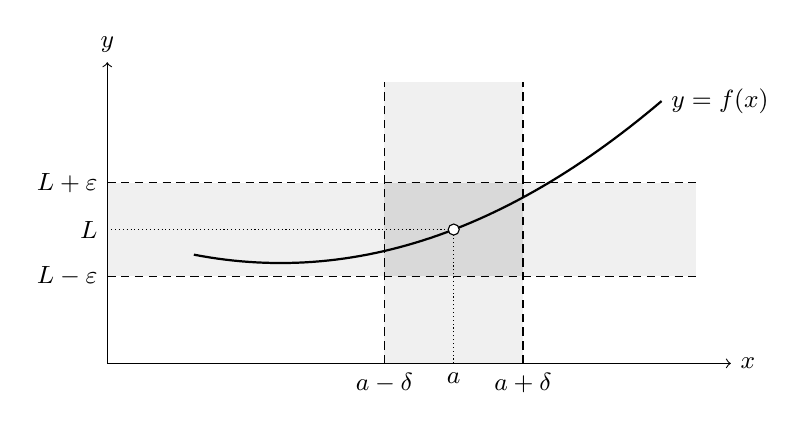
\begin{tikzpicture}[x=2.2cm,y=1.7cm,font=\small]
\fill[gray!12] (0,0.65) rectangle (3.4,1.35);
\fill[gray!12] (1.6,0) rectangle (2.4,2.1);
\fill[gray!30] (1.6,0.65) rectangle (2.4,1.35);
\draw[->] (0,0)--(3.6,0) node[right] {$x$};
\draw[->] (0,0)--(0,2.25) node[above] {$y$};
\draw[densely dashed] (0,0.65)--(3.4,0.65);
\draw[densely dashed] (0,1.35)--(3.4,1.35);
\draw[densely dotted] (0,1)--(2,1);
\draw[densely dashed] (1.6,0)--(1.6,2.1);
\draw[densely dashed] (2.4,0)--(2.4,2.1);
\draw[densely dotted] (2,0)--(2,1);
\draw[thick,domain=0.5:3.2,samples=60] plot (\x,{1+0.5*(\x-2)+0.25*(\x-2)^2});
\fill[white] (2,1) circle (2pt);
\draw (2,1) circle (2pt);
\node[left] at (0,1.35) {$L+\varepsilon$};
\node[left] at (0,1) {$L$};
\node[left] at (0,0.65) {$L-\varepsilon$};
\node[below] at (1.6,0) {$a-\delta$};
\node[below] at (2,0) {$a$};
\node[below] at (2.4,0) {$a+\delta$};
\node[right] at (3.2,1.96) {$y=f(x)$};
\end{tikzpicture}
\end{center}
\begin{example}
\textnormal{(课堂例题: 有限点处的定义法)} 用定义证明
\[
\lim_{x\to2}\frac{x^2-4}{x-2}=4,\qquad\lim_{x\to2}\frac{x-2}{x^2-4}=\frac14.
\]
\end{example}
\par\indent\textbf{分析:} 两个函数在 $x=2$ 处都没有定义, 但极限只考察 $x\ne2$ 的点, 在那里可以约去公因式 $x-2$. 第一个函数化为 $x+2$, 误差 $|(x+2)-4|=|x-2|$, 取 $\delta=\varepsilon$ 即可.

第二个函数在 $x\ne\pm2$ 时化为 $\displaystyle\frac1{x+2}$, 误差为
\[
\left|\frac1{x+2}-\frac14\right|=\frac{|x-2|}{4|x+2|}.
\]
分子是可以用 $\delta$ 控制的距离 $|x-2|$, 但分母随 $x$ 变化. 在 $x=-2$ 附近, $\displaystyle\frac1{|x+2|}$ 可以任意大, 所以在整个定义域上, 误差不能用 $|x-2|$ 的常数倍来控制. 不过只需考虑 $2$ 附近的 $x$, 可以先把 $x$ 限制在 $|x-2|<1$ 的范围内. 这时 $1<x<3$, 所以 $x+2>3$. 分母 $4|x+2|$ 有了下界 $12$, 误差就小于 $\displaystyle\frac{|x-2|}{12}$. 再要求 $|x-2|<12\varepsilon$, 误差就小于 $\varepsilon$. 要使两个要求同时满足, 取 $\delta=\min\{1,12\varepsilon\}$ 即可. 限制的半径取 $1$ 只是为了方便. 只要半径 $r<4$, 范围 $|x-2|<r$ 就不含使分母为零的点 $-2$, 并且其中 $x+2>4-r>0$, 同样可行.
\begin{cnproof}
任给 $\varepsilon>0$, 取 $\delta=\varepsilon$. 当 $0<|x-2|<\delta$ 时 $x\ne2$, 所以
\[
\left|\frac{x^2-4}{x-2}-4\right|=|(x+2)-4|=|x-2|<\varepsilon.
\]

任给 $\varepsilon>0$, 取 $\delta=\min\{1,12\varepsilon\}$. 当 $0<|x-2|<\delta$ 时, $|x-2|<1$, 故 $x+2>3$, $x^2-4=(x-2)(x+2)\ne0$, 并且
\[
\left|\frac{x-2}{x^2-4}-\frac14\right|=\left|\frac1{x+2}-\frac14\right|=\frac{|x-2|}{4(x+2)}<\frac{|x-2|}{12}<\varepsilon.
\]
两个极限都由定义得证.
\end{cnproof}
\begin{example}\label{ex:5-2}
\textnormal{(教材例5.2)} 设 $m\in\mathbb N^+$, 证明 $\displaystyle\lim_{x\to a}x^m=a^m$.
\end{example}
\par\indent\textbf{分析:} 要把误差 $|x^m-a^m|$ 与 $|x-a|$ 联系起来, 可以从 $x^m-a^m$ 中分解出因式 $x-a$:
\[
x^m-a^m=(x-a)\left(x^{m-1}+x^{m-2}a+\cdots+xa^{m-2}+a^{m-1}\right).
\]
把右边乘开, 中间的项正负相消, 只剩下 $x^m-a^m$. $m\ge2$ 时第二个因式随 $x$ 变化, 并且在整个数轴上无界. 但只需考虑 $a$ 附近的 $x$, 所以先把 $x$ 限制在 $|x-a|<1$ 内, 求出这个因式的一个与 $x$ 无关的界. 这时 $|x|\le|x-a|+|a|<|a|+1$. 第二个因式共有 $m$ 项, 每一项形如 $x^{m-1-j}a^j$, 其绝对值不超过 $(|a|+1)^{m-1-j}(|a|+1)^j=(|a|+1)^{m-1}$, 于是
\[
|x^m-a^m|\le m(|a|+1)^{m-1}|x-a|.
\]
记 $K=m(|a|+1)^{m-1}$. 要使 $K|x-a|<\varepsilon$, 只需 $\displaystyle|x-a|<\frac\varepsilon K$. 再加上开始时的限制 $|x-a|<1$, 取 $\displaystyle\delta=\min\left\{1,\frac\varepsilon K\right\}$.
\begin{cnproof}
记 $K=m(|a|+1)^{m-1}$. 任给 $\varepsilon>0$, 取 $\displaystyle\delta=\min\left\{1,\frac\varepsilon K\right\}$. 当 $0<|x-a|<\delta$ 时, $|x|\le|x-a|+|a|<|a|+1$, 所以第二个因式中每一项 $x^{m-1-j}a^j$ ($j=0,1,\ldots,m-1$) 的绝对值不超过 $(|a|+1)^{m-1}$, 从而
\[
|x^m-a^m|\le K|x-a|<K\cdot\frac\varepsilon K=\varepsilon.
\]
故 $\displaystyle\lim_{x\to a}x^m=a^m$.
\end{cnproof}
\begin{example}
\textnormal{(指定作业: 习题1.5第1题(4))} 设 $a>0$, 用定义证明 $\displaystyle\lim_{x\to a}\sqrt x=\sqrt a$.
\end{example}
\par\indent\textbf{分析:} 要从误差 $\sqrt x-\sqrt a$ 中分出因子 $x-a$, 可以把它分子有理化, 由平方差公式得
\[
|\sqrt x-\sqrt a|=\frac{|x-a|}{\sqrt x+\sqrt a}\le\frac{|x-a|}{\sqrt a},
\]
后一步去掉了分母中非负的 $\sqrt x$. 误差已经不超过 $|x-a|$ 的常数倍, 不需要先限制邻域来求界. 唯一的限制来自定义域. $\sqrt x$ 只在 $x\ge0$ 时有意义, 而 $|x-a|<a$ 时 $x>0$, 所以半径不超过 $a$ 即可. 要使 $\displaystyle\frac{|x-a|}{\sqrt a}<\varepsilon$, 只需 $|x-a|<\sqrt a\,\varepsilon$. 两个要求合起来, 取 $\delta=\min\{a,\sqrt a\,\varepsilon\}$.
\begin{cnproof}
任给 $\varepsilon>0$, 取 $\delta=\min\{a,\sqrt a\,\varepsilon\}$. 当 $0<|x-a|<\delta$ 时 $x>0$, 并且
\[
|\sqrt x-\sqrt a|=\frac{|x-a|}{\sqrt x+\sqrt a}\le\frac{|x-a|}{\sqrt a}<\varepsilon.
\]
故 $\displaystyle\lim_{x\to a}\sqrt x=\sqrt a$.
\end{cnproof}
\par\indent\textbf{方法小结:} 用定义证明函数极限时, 寻找 $A$ 或 $\delta$ 的办法与寻找 $N$ 相同, 都是先写出误差并化简, 再从误差小于 $\varepsilon$ 倒推出自变量应满足的条件. 直接解出的阈值可能不是正数, 如 $\varepsilon\ge1$ 时的 $-\ln\varepsilon$, 这时取它与 $1$ 中的较大者, 或者对较大的 $\varepsilon$ 单独处理. $x\to\infty$ 时用 $|x|$ 估计误差; 分母需要下界时, 可以用反三角不等式给出只含 $|x|$ 的下界, 如 $|2x-1|\ge2|x|-1$. $x\to a$ 时, 先把误差写成 $|x-a|$ 乘以一个因子, 再求这个因子的一个与 $x$ 无关的界 $K$. 若因子在整个定义域上无界, 就把 $x$ 限制在 $a$ 的一个固定邻域内求界, 常用 $|x-a|<1$; 若这个范围内有使函数没有定义或使分母为零的点, 就改用能避开这些点的较小邻域. 因子的界只在这个邻域内成立, 所以 $\delta$ 要取为邻域的半径与 $\displaystyle\frac\varepsilon K$ 中的较小者. $A$ 与 $\delta$ 都只能依赖于 $\varepsilon$ 和题中给定的量, 不能依赖于 $x$.
\subsection{单侧极限}
有时需要单独考察 $x$ 从一侧接近 $a$ 的情形. 例如 $\sqrt x$ 只在 $x\ge0$ 时有定义, 在 $0$ 处只能考察 $x$ 从右侧接近 $0$. 分段函数在分段点两侧的表达式不同, 也常常需要分别考察两侧.
\begin{definition}
设 $f$ 在区间 $(a-r,a)$ 内有定义, $L$ 是实数. 若对任意 $\varepsilon>0$, 都存在 $\delta>0$ ($\delta\le r$), 使当 $a-\delta<x<a$ 时恒有 $|f(x)-L|<\varepsilon$, 则称 $L$ 为 $f$ 在 $a$ 处的\textbf{左极限}, 记作 $\displaystyle\lim_{x\to a^-}f(x)=L$ 或 $f(a^-)=L$. 把区间换成 $(a,a+r)$, 条件换成 $a<x<a+\delta$, 就得到\textbf{右极限}的定义, 记作 $\displaystyle\lim_{x\to a^+}f(x)=L$ 或 $f(a^+)=L$.
\end{definition}
\begin{theorem}\label{thm:5-onesided}
$\displaystyle\lim_{x\to a}f(x)=L$ 的充分必要条件是 $f$ 在 $a$ 处的左、右极限都存在并且都等于 $L$.
\end{theorem}
\begin{cnproof}
去心邻域 $0<|x-a|<\delta$ 由 $a-\delta<x<a$ 与 $a<x<a+\delta$ 两部分组成. 若双侧极限成立, 把定义中的 $x$ 限制在其中一部分, 就得到相应的单侧极限. 反过来, 任给 $\varepsilon>0$, 由左、右极限分别有 $\delta_1,\delta_2>0$, 使 $a-\delta_1<x<a$ 时及 $a<x<a+\delta_2$ 时都有 $|f(x)-L|<\varepsilon$. 取 $\delta=\min\{\delta_1,\delta_2\}$, 则当 $0<|x-a|<\delta$ 时, 或者 $a-\delta_1\le a-\delta<x<a$, 或者 $a<x<a+\delta\le a+\delta_2$, 总有 $|f(x)-L|<\varepsilon$.
\end{cnproof}
与数列一样, 函数的极限若存在则是唯一的. 设当 $x\to a$ 时 $f(x)$ 既以 $L$ 为极限, 又以 $K$ 为极限. 任给 $\varepsilon>0$, 由这两个极限的定义, 分别有 $\delta_1,\delta_2>0$, 使 $0<|x-a|<\delta_1$ 时 $|f(x)-L|<\varepsilon$, $0<|x-a|<\delta_2$ 时 $|f(x)-K|<\varepsilon$. 任取满足 $0<|x-a|<\min\{\delta_1,\delta_2\}$ 的 $x$, 则
\[
|L-K|\le|L-f(x)|+|f(x)-K|<2\varepsilon.
\]
$|L-K|$ 是与 $\varepsilon$ 无关的非负数, 却对任意 $\varepsilon>0$ 都小于 $2\varepsilon$, 只能等于 $0$, 故 $L=K$. 自变量趋于无穷以及单侧极限的情形同样如此.
\begin{example}\label{ex:5-sgn}
\textnormal{(教材正文示例)} 讨论符号函数
\[
\operatorname{sgn}x=\begin{cases}1,&x>0,\\0,&x=0,\\-1,&x<0\end{cases}
\]
当 $x\to0$ 时的极限.
\end{example}
\begin{cnsolution}
当 $x>0$ 时 $\operatorname{sgn}x=1$, 所以对任意 $\varepsilon>0$, 任取 $\delta>0$, 当 $0<x<\delta$ 时都有 $|\operatorname{sgn}x-1|=0<\varepsilon$. 故右极限为 $1$. 同理, 左极限为 $-1$. 若 $\displaystyle\lim_{x\to0}\operatorname{sgn}x$ 存在, 设为 $L$. 由定理\ref{thm:5-onesided}, 左、右极限都等于 $L$; 再由单侧极限的唯一性, $L=-1$ 且 $L=1$, 矛盾. 所以 $\displaystyle\lim_{x\to0}\operatorname{sgn}x$ 不存在. 函数值 $\operatorname{sgn}0=0$ 不参与这一判断.
\end{cnsolution}
讨论分段函数在分段点处的极限时, 一般先分别求两侧的极限, 再比较它们是否相等.
\begin{example}\label{ex:h15-1-5}
\textnormal{(指定作业: 习题1.5第1题(5))} 用定义证明 $\displaystyle\lim_{x\to0^-}2^{\frac1x}=0$.
\end{example}
\par\indent\textbf{分析:} 当 $x<0$ 时 $2^{\frac1x}$ 是小于 $1$ 的正数, 误差就是它本身. 若 $\varepsilon\ge1$, 一切 $x<0$ 都满足要求, 取 $\delta=1$ 即可. 设 $0<\varepsilon<1$. 目标 $2^{\frac1x}<\varepsilon$ 等价于 $\displaystyle\frac1x<\log_2\varepsilon$. 由此直接解 $x$ 要对负数取倒数, 不等号的方向容易弄错, 所以改用 $|x|$ 来写. 当 $x<0$ 时 $\displaystyle\frac1x=-\frac1{|x|}$, 所以 $\displaystyle2^{\frac1x}=\frac1{2^{\frac1{|x|}}}$, 目标变成 $\displaystyle2^{\frac1{|x|}}>\frac1\varepsilon$, 即 $\displaystyle\frac1{|x|}>\log_2\frac1\varepsilon$. 由 $0<\varepsilon<1$, 右边是正数, 两边取倒数得 $\displaystyle|x|<\frac1{\log_2\frac1\varepsilon}$.
\begin{cnproof}
任给 $\varepsilon>0$. 若 $\varepsilon\ge1$, 取 $\delta=1$, 则 $-\delta<x<0$ 时 $0<2^{\frac1x}<1\le\varepsilon$. 若 $0<\varepsilon<1$, 取 $\displaystyle\delta=\frac1{\log_2\frac1\varepsilon}$, 它是正数. 当 $-\delta<x<0$ 时 $0<|x|<\delta$, 所以 $\displaystyle\frac1{|x|}>\log_2\frac1\varepsilon$. 由指数函数严格增加, $\displaystyle2^{\frac1{|x|}}>\frac1\varepsilon$, 从而
\[
\left|2^{\frac1x}-0\right|=\frac1{2^{\frac1{|x|}}}<\varepsilon.
\]
故 $\displaystyle\lim_{x\to0^-}2^{\frac1x}=0$.
\end{cnproof}
\begin{example}\label{ex:h15-3}
\textnormal{(指定作业: 习题1.5第3题)} 设 $x_0>0$, 用单侧极限证明 $\displaystyle\lim_{x\to x_0}\ln x=\ln x_0$.
\end{example}
\par\indent\textbf{分析:} 目标 $|\ln x-\ln x_0|<\varepsilon$ 就是 $\ln x_0-\varepsilon<\ln x<\ln x_0+\varepsilon$. 由指数函数严格增加, 它等价于 $e^{\ln x_0-\varepsilon}<x<e^{\ln x_0+\varepsilon}$, 即
\[
x_0e^{-\varepsilon}<x<x_0e^{\varepsilon}.
\]
这个区间包含 $x_0$, 其中 $x_0$ 左边的部分长 $x_0(1-e^{-\varepsilon})$, 右边的部分长 $x_0(e^\varepsilon-1)$. 两者不相等, 所以它不是以 $x_0$ 为中心的邻域. 按题目的要求分别考察两侧, 每一侧直接取这一侧的长度作为 $\delta$, 最后由单侧极限与双侧极限的关系把两侧合起来.
\begin{cnproof}
任给 $\varepsilon>0$. 取 $\delta_1=x_0(1-e^{-\varepsilon})$, 它是小于 $x_0$ 的正数. 当 $x_0-\delta_1<x<x_0$ 时, $x_0e^{-\varepsilon}<x<x_0$, 所以 $x>0$, 且由对数函数严格增加, $\ln x_0-\varepsilon<\ln x<\ln x_0$, 即 $|\ln x-\ln x_0|<\varepsilon$. 故左极限为 $\ln x_0$.

取 $\delta_2=x_0(e^{\varepsilon}-1)>0$. 当 $x_0<x<x_0+\delta_2$ 时, $x_0<x<x_0e^{\varepsilon}$, 同理 $\ln x_0<\ln x<\ln x_0+\varepsilon$. 故右极限也为 $\ln x_0$.

左、右极限都等于 $\ln x_0$, 所以 $\displaystyle\lim_{x\to x_0}\ln x=\ln x_0$.
\end{cnproof}
也可以取 $\delta_1,\delta_2$ 中较小者作为双侧的半径, 直接验证双侧极限.
\subsection{极限的否定形式}
与数列的情形一样, 把定义中的“对任意 $\varepsilon>0$”“都存在 $\delta>0$”“当 $0<|x-a|<\delta$ 时恒有 $|f(x)-L|<\varepsilon$”依次否定, 就得到“当 $x\to a$ 时 $f(x)$ 不以 $L$ 为极限”的准确表述: 存在 $\varepsilon_0>0$, 使对每个 $\delta>0$, 都有某个 $x$ 满足
\[
0<|x-a|<\delta\qquad\text{且}\qquad|f(x)-L|\ge\varepsilon_0.
\]
也就是说, 有一个固定的误差限度 $\varepsilon_0$, 无论 $\delta$ 多么小, 在去心邻域 $\mathring U(a,\delta)$ 中总能找到使 $|f(x)-L|\ge\varepsilon_0$ 的点 $x$; 这样的点可以随 $\delta$ 改变. 要证明极限不存在, 须对每个实数 $L$ 作出这样的论证. 其他变化方式下的否定形式可以类似地写出.
\begin{example}
\textnormal{(指定作业: 习题1.5第2题)} 证明 $\displaystyle\lim_{x\to0}\frac x{|x|}$ 不存在.
\end{example}
\par\indent\textbf{分析:} 当 $x\ne0$ 时 $\displaystyle\frac x{|x|}=\operatorname{sgn}x$, 由例\ref{ex:5-sgn} 即知极限不存在. 这里直接用否定形式证明, 以熟悉量词的写法. 对候选值 $L$, 要选定一个误差 $\varepsilon_0$, 并在每个去心邻域中找出函数值与 $L$ 相距不小于 $\varepsilon_0$ 的点. 函数只取 $1$ 与 $-1$ 两个值, 它们相距 $2$, 任何 $L$ 到其中至少一个的距离不小于 $1$. 所以取 $\varepsilon_0=1$, 在函数值离 $L$ 较远的那一侧取点.
\begin{cnproof}
任取 $L\in\mathbb R$, 令 $\varepsilon_0=1$, 并任给 $\delta>0$. 若 $L\ge0$, 取 $\displaystyle x=-\frac\delta2$, 则 $0<|x|<\delta$, 且
\[
\left|\frac x{|x|}-L\right|=|-1-L|=1+L\ge1.
\]
若 $L<0$, 取 $\displaystyle x=\frac\delta2$, 则 $0<|x|<\delta$, 且 $\displaystyle\left|\frac x{|x|}-L\right|=1-L>1$. 所以 $L$ 不是极限. 由 $L$ 的任意性, 极限不存在.
\end{cnproof}
\section{函数极限的性质与收敛准则}
1.5 节用定义证明函数极限, 每个极限都要单独选取 $\delta$ 或 $A$. 本节把数列极限的性质和运算法则推广到函数极限, 并建立两个重要极限. 此后, 大多数函数极限可以通过恒等变形和已知的极限算出. 叙述以 $x\to a$ 为代表, 默认函数在 $a$ 的某个去心邻域内有定义. 对单侧极限和自变量趋于无穷的情形, 只需把去心邻域换成相应的范围, 结论和证明都相同.
\subsection{函数极限的局部性质}
函数极限只涉及 $a$ 附近的函数值, 由它推出的有界、保序、保号等性质也只在 $a$ 的某个去心邻域内成立, 所以称为\textbf{局部性质}. 证明的思路与 1.3 节数列的情形相同, 只是把“$n>N$”换成“$0<|x-a|<\delta$”; 合并几个条件时, 取最大的 $N$ 改为取最小的 $\delta$.
\begin{theorem}[局部性质]
设 $\displaystyle\lim_{x\to a}f(x)=L$. 则:

\textup{(1)} (唯一性) 极限 $L$ 是唯一的;

\textup{(2)} (局部有界性) 存在 $\delta>0$ 和 $M>0$, 使 $0<|x-a|<\delta$ 时 $|f(x)|\le M$;

\textup{(3)} (保序性) 设还有 $\displaystyle\lim_{x\to a}g(x)=K$. 若 $L>K$, 则存在 $\delta>0$, 使 $0<|x-a|<\delta$ 时 $f(x)>g(x)$; 若在 $a$ 的某个去心邻域内 $f(x)\ge g(x)$, 则 $L\ge K$;

\textup{(4)} (保号性) 若 $L\ne0$, 则存在 $\delta>0$, 使 $0<|x-a|<\delta$ 时 $f(x)$ 与 $L$ 同号, 并且 $\displaystyle|f(x)|>\frac{|L|}2$.
\end{theorem}
\begin{cnproof}
(1) 已在 1.5 节证明.

(2) 对 $\varepsilon=1$ 取 $\delta$, 则 $0<|x-a|<\delta$ 时 $|f(x)|\le|f(x)-L|+|L|<|L|+1$, 取 $M=|L|+1$.

(3) 设 $L>K$, 对 $\displaystyle\varepsilon=\frac{L-K}2$ 分别取两个函数的半径, 再取其中较小者 $\delta$, 则 $0<|x-a|<\delta$ 时
\[
f(x)>L-\varepsilon=\frac{L+K}2=K+\varepsilon>g(x).
\]
若在 $\mathring U(a,\delta_1)$ 内 $f(x)\ge g(x)$ 而 $L<K$, 由刚证的结论 (交换 $f$ 与 $g$ 的位置), 存在 $\delta_2>0$, 使 $0<|x-a|<\delta_2$ 时 $f(x)<g(x)$. 于是满足 $0<|x-a|<\min\{\delta_1,\delta_2\}$ 的 $x$ 同时使 $f(x)\ge g(x)$ 与 $f(x)<g(x)$ 成立, 矛盾.

(4) 对 $\displaystyle\varepsilon=\frac{|L|}2$ 取 $\delta$, 则 $0<|x-a|<\delta$ 时, 由反三角不等式 $\displaystyle|f(x)|\ge|L|-|f(x)-L|>\frac{|L|}2$; 并且 $L>0$ 时 $\displaystyle f(x)>L-\frac L2>0$, $L<0$ 时 $\displaystyle f(x)<L+\frac{|L|}2=\frac L2<0$.
\end{cnproof}
局部有界性只说明 $f$ 在 $a$ 附近有界, 与 $f(a)$ 无关, 也不能推出 $f$ 在整个定义域上有界. 收敛数列的全部项有界, 是因为分界以前只有有限多项; 而去心邻域以外可能有无穷多个点, 函数在那里可以无界. 例如 1.5 节已证 $\displaystyle\lim_{x\to2}\frac{x-2}{x^2-4}=\frac14$, 这个函数在 $2$ 附近有界, 它的绝对值在 $-2$ 附近却可以任意大.

与数列的情形一样, 保序性的后一个结论中, 即使条件是严格的 $f(x)>g(x)$, 也只能得到 $L\ge K$. 例如 $x\ne0$ 时 $x^2>0$, 而 $\displaystyle\lim_{x\to0}x^2=0$.
\begin{example}\label{ex:k16-1}
\textnormal{(课堂例题: 根式极限的条件)} 设 $\displaystyle\lim_{x\to a}f(x)=b$, 且在 $a$ 的某个去心邻域内 $f(x)\ge0$. 证明 $\displaystyle\lim_{x\to a}\sqrt{f(x)}=\sqrt b$.
\end{example}
\par\indent\textbf{分析:} 先由保序性 (与常数 $0$ 比较) 得 $b\ge0$, 所以 $\sqrt b$ 有意义. 设 $b>0$, 这时共轭式 $\sqrt{f(x)}+\sqrt b\ge\sqrt b>0$. 目标误差乘以共轭式, 得
\[
\bigl|\sqrt{f(x)}-\sqrt b\bigr|=\frac{|f(x)-b|}{\sqrt{f(x)}+\sqrt b}.
\]
分子是已知能控制的 $|f(x)-b|$, 分母不小于 $\sqrt b$, 所以误差不超过 $\displaystyle\frac{|f(x)-b|}{\sqrt b}$. 要使它小于 $\varepsilon$, 只需 $|f(x)-b|<\sqrt b\,\varepsilon$. 当 $b=0$ 时分母可能为零, 不能这样估计. 但这时目标 $\sqrt{f(x)}<\varepsilon$ 就是 $f(x)<\varepsilon^2$, 可由 $f(x)\to0$ 直接得到. 两种情形下, 半径都不能超过 $f(x)\ge0$ 成立的那个邻域的半径, 否则根式可能没有意义.
\begin{cnproof}
设 $0<|x-a|<\delta_0$ 时 $f(x)\ge0$. 由保序性, $b\ge0$. 任给 $\varepsilon>0$.

若 $b>0$, 由 $f(x)\to b$, 存在 $\delta_1>0$, 使 $0<|x-a|<\delta_1$ 时 $|f(x)-b|<\sqrt b\,\varepsilon$. 取 $\delta=\min\{\delta_0,\delta_1\}$, 则 $0<|x-a|<\delta$ 时
\[
\bigl|\sqrt{f(x)}-\sqrt b\bigr|=\frac{|f(x)-b|}{\sqrt{f(x)}+\sqrt b}\le\frac{|f(x)-b|}{\sqrt b}<\varepsilon.
\]

若 $b=0$, 存在 $\delta_1>0$, 使 $0<|x-a|<\delta_1$ 时 $|f(x)|<\varepsilon^2$. 取 $\delta=\min\{\delta_0,\delta_1\}$, 则 $0<|x-a|<\delta$ 时 $0\le f(x)<\varepsilon^2$, 故 $\bigl|\sqrt{f(x)}-0\bigr|<\varepsilon$.

两种情形都有 $\displaystyle\lim_{x\to a}\sqrt{f(x)}=\sqrt b$.
\end{cnproof}
\subsection{海涅定理与运算法则}
数列极限的运算法则、两边夹定理等结论, 可以借助下面的海涅定理推广到函数. 这个定理的意思是, 当 $x\to a$ 时 $f(x)\to L$, 等价于沿任何一列趋于 $a$ 而各项都不等于 $a$ 的点, 函数值都趋于 $L$. 要求各项不等于 $a$, 是因为函数极限与 $f(a)$ 无关.
\begin{theorem}[海涅定理]
设 $f$ 在 $\mathring U(a,r)$ 内有定义. 则 $\displaystyle\lim_{x\to a}f(x)=L$ 的充分必要条件是: 对 $\mathring U(a,r)$ 中任意一个收敛于 $a$ 的数列 $\{x_n\}$, 都有 $\displaystyle\lim_{n\to\infty}f(x_n)=L$.
\end{theorem}
\par\indent\textbf{分析:} 必要性可以由定义直接推出, 因为 $a$ 附近 (不含 $a$) 的点都满足 $|f(x)-L|<\varepsilon$, 而数列中靠后的各项都是这样的点. 充分性要从“沿每一列点都成立”推出函数极限. 条件只涉及一列一列的点, 没有给出任何半径, 难以直接找出 $\delta$. 所以用反证法, 看函数极限不成立时能造出怎样的数列. 按否定形式, 函数极限不成立意味着有一个固定的 $\varepsilon_0$, 无论半径多么小, 去心邻域中总有函数值与 $L$ 相距不小于 $\varepsilon_0$ 的点. 让半径依次取 $\displaystyle1,\frac12,\frac13,\ldots$, 每次取出一个这样的点, 就得到一列趋于 $a$ 的点. 这些点的函数值与 $L$ 的距离都不小于 $\varepsilon_0$, 不趋于 $L$, 与条件矛盾.
\begin{cnproof}
必要性. 设 $\displaystyle\lim_{x\to a}f(x)=L$, $\{x_n\}$ 是 $\mathring U(a,r)$ 中收敛于 $a$ 的数列. 任给 $\varepsilon>0$, 存在 $\delta>0$, 使 $0<|x-a|<\delta$ 时 $|f(x)-L|<\varepsilon$. 由 $x_n\to a$, 存在 $N$, 使 $n>N$ 时 $|x_n-a|<\delta$; 又 $x_n\ne a$, 所以 $0<|x_n-a|<\delta$, 从而 $|f(x_n)-L|<\varepsilon$. 故 $f(x_n)\to L$.

充分性. 反设条件成立而 $f(x)$ 不以 $L$ 为极限. 由否定形式, 存在 $\varepsilon_0>0$, 使对每个 $\delta>0$ 都有 $x$ 满足 $0<|x-a|<\delta$ 且 $|f(x)-L|\ge\varepsilon_0$. 对 $n=1,2,\ldots$, 取 $\displaystyle\delta=\min\left\{r,\frac1n\right\}$, 把相应的点记为 $x_n$, 则
\[
0<|x_n-a|<\frac1n,\qquad|f(x_n)-L|\ge\varepsilon_0.
\]
由 $\delta\le r$ 知 $x_n\in\mathring U(a,r)$, 由前一式及两边夹定理知 $x_n\to a$, 所以 $\{x_n\}$ 是 $\mathring U(a,r)$ 中收敛于 $a$ 的数列; 由后一式, $\{f(x_n)\}$ 不收敛于 $L$. 这与条件矛盾.
\end{cnproof}
海涅定理对单侧极限和自变量趋于无穷的情形同样成立, 证明也类似, 只是所取的数列要相应改变. 对单侧极限, 把数列限制在 $a$ 的相应一侧. 对 $x\to+\infty$, 改为考虑满足 $x_n\to+\infty$ 的数列, 这里 $x_n\to+\infty$ 表示对任意 $M>0$, 从某项起都有 $x_n>M$. $x\to-\infty$ 与 $x\to\infty$ 的情形也这样处理.
\begin{theorem}[四则运算法则]
设 $\displaystyle\lim_{x\to a}f(x)=L$, $\displaystyle\lim_{x\to a}g(x)=K$. 则
\[
\lim_{x\to a}\bigl(f(x)\pm g(x)\bigr)=L\pm K,\qquad\lim_{x\to a}f(x)g(x)=LK;
\]
若还有 $K\ne0$, 则 $g(x)$ 在 $a$ 的某个去心邻域内不为零, 并且 $\displaystyle\lim_{x\to a}\frac{f(x)}{g(x)}=\frac LK$.
\end{theorem}
\begin{cnproof}
设 $f$ 与 $g$ 都在 $\mathring U(a,r)$ 内有定义, $\{x_n\}$ 是其中任意一个收敛于 $a$ 的数列. 由海涅定理的必要性, $f(x_n)\to L$, $g(x_n)\to K$; 由数列极限的四则运算法则, $f(x_n)\pm g(x_n)\to L\pm K$, $f(x_n)g(x_n)\to LK$. 再由海涅定理的充分性, 前两个结论成立.

设 $K\ne0$. 由保号性, 存在 $\delta_0\in(0,r]$, 使 $0<|x-a|<\delta_0$ 时 $g(x)\ne0$, 商 $\displaystyle\frac{f(x)}{g(x)}$ 在 $\mathring U(a,\delta_0)$ 内有定义. 对其中任意一个收敛于 $a$ 的数列 $\{x_n\}$, 由数列的商的法则, $\displaystyle\frac{f(x_n)}{g(x_n)}\to\frac LK$, 再由海涅定理得到商的结论.
\end{cnproof}
取 $g$ 为常数函数, 就得到常数倍的法则. 使用这些法则时, 必须先确认各部分的极限存在, 商的情形还要确认分母的极限不为零. 分子、分母都趋于零的商不能直接用商的法则, 要先变形.
\begin{theorem}[复合函数的极限]
设 $\displaystyle\lim_{x\to a}g(x)=b$, $\displaystyle\lim_{u\to b}f(u)=B$, 并且在 $a$ 的某个去心邻域 $\mathring U(a,\delta_0)$ 内, $g(x)\ne b$, 复合函数 $f(g(x))$ 有定义. 则 $\displaystyle\lim_{x\to a}f(g(x))=B$.
\end{theorem}
\par\indent\textbf{分析:} 目标是 $|f(g(x))-B|<\varepsilon$. 由外层的极限, 存在 $\eta>0$, 只要 $u$ 满足 $0<|u-b|<\eta$, 就有 $|f(u)-B|<\varepsilon$. 所以只需让 $u=g(x)$ 落在去心邻域 $\mathring U(b,\eta)$ 中, 即 $|g(x)-b|<\eta$ 且 $g(x)\ne b$. 只要 $x$ 离 $a$ 足够近, 内层的极限就保证前一个要求; 后一个要求由条件保证. 因此选取半径时, 先由 $\varepsilon$ 确定外层的 $\eta$, 再由 $\eta$ 确定内层的 $\delta$.
\begin{cnproof}
任给 $\varepsilon>0$. 由 $\displaystyle\lim_{u\to b}f(u)=B$, 存在 $\eta>0$, 使 $0<|u-b|<\eta$ 时 $|f(u)-B|<\varepsilon$. 对这个 $\eta$, 由 $\displaystyle\lim_{x\to a}g(x)=b$, 存在 $\delta_1>0$, 使 $0<|x-a|<\delta_1$ 时 $|g(x)-b|<\eta$. 取 $\delta=\min\{\delta_0,\delta_1\}$. 当 $0<|x-a|<\delta$ 时, $u=g(x)$ 满足 $0<|u-b|<\eta$, 所以 $|f(g(x))-B|<\varepsilon$.
\end{cnproof}
这个定理是换元的依据. 求 $\displaystyle\lim_{x\to a}f(g(x))$ 时, 令 $u=g(x)$, 只要验证 $u\to b$, 并且 $a$ 附近 $x\ne a$ 时 $u\ne b$, 就可以改求 $\displaystyle\lim_{u\to b}f(u)$. 若 $x$ 在 $a$ 附近时 $g(x)$ 总在 $b$ 的同一侧 (例如总有 $g(x)>b$), 定理中外层的极限可以换成相应的单侧极限.

条件 $g(x)\ne b$ 不能随意去掉, 因为外层的极限与 $f(b)$ 无关, 而 $g(x)=b$ 时 $f(g(x))$ 恰好等于 $f(b)$. 例如 $f(u)=1$ ($u\ne0$), $f(0)=0$, 而 $g(x)\equiv0$, 则 $\displaystyle\lim_{u\to0}f(u)=1$, 但 $f(g(x))\equiv0$. 若 $f$ 在 $b$ 处有定义且 $f(b)=B$, 则 $g(x)=b$ 的点也满足 $|f(g(x))-B|=0<\varepsilon$, 这时可以去掉条件 $g(x)\ne b$.
\begin{example}
\textnormal{(教材例6.1)} 求 $\displaystyle\lim_{x\to+\infty}\left(\sqrt{x^2+4x}-\sqrt{x^2+3}\right)$, 再求 $x\to-\infty$ 时的极限, 并判断 $x\to\infty$ 时极限是否存在.
\end{example}
\par\indent\textbf{分析:} 两个根式都无限增大, 不能用差的法则. 两个很大的数之差可能很小, 也可能很大, 要看两项能否相互抵消. 根号内的 $x^2$ 不能直接相减, 所以先乘以共轭式, 由平方差公式把差化成一个分式:
\[
\sqrt{x^2+4x}-\sqrt{x^2+3}=\frac{(x^2+4x)-(x^2+3)}{\sqrt{x^2+4x}+\sqrt{x^2+3}}=\frac{4x-3}{\sqrt{x^2+4x}+\sqrt{x^2+3}},
\]
$x^2$ 在分子中消去了. 现在分子、分母都与 $|x|$ 大小相当, 同除以 $|x|$ 后都有有限的极限. 把 $|x|$ 除进根号时要用 $|x|=\sqrt{x^2}$, 例如 $\displaystyle\frac{\sqrt{x^2+4x}}{|x|}=\sqrt{1+\frac4x}$. 分子 $4x-3$ 除以 $|x|$ 时要看 $x$ 的符号: $x>0$ 时得 $\displaystyle4-\frac3x$, $x<0$ 时得 $\displaystyle-4+\frac3x$. 两个方向的结果因此不同.
\begin{cnsolution}
当 $x>0$ 时, 有理化后以 $x=\sqrt{x^2}$ 同除分子、分母, 得
\[
\begin{aligned}
\lim_{x\to+\infty}\left(\sqrt{x^2+4x}-\sqrt{x^2+3}\right)
&=\lim_{x\to+\infty}\frac{4x-3}{\sqrt{x^2+4x}+\sqrt{x^2+3}}\\
&=\lim_{x\to+\infty}\frac{4-\frac3x}{\sqrt{1+\frac4x}+\sqrt{1+\frac3{x^2}}}=\frac4{1+1}=2,
\end{aligned}
\]
其中根式的极限由本节例\ref{ex:k16-1} 得到. 当 $x<-4$ 时 $x^2+4x>0$, 并且 $\sqrt{x^2}=-x$, 以 $-x$ 同除分子、分母, 得
\[
\begin{aligned}
\lim_{x\to-\infty}\left(\sqrt{x^2+4x}-\sqrt{x^2+3}\right)
&=\lim_{x\to-\infty}\frac{4x-3}{\sqrt{x^2+4x}+\sqrt{x^2+3}}\\
&=\lim_{x\to-\infty}\frac{-4+\frac3x}{\sqrt{1+\frac4x}+\sqrt{1+\frac3{x^2}}}=\frac{-4}{1+1}=-2.
\end{aligned}
\]
两个方向的极限分别为 $2$ 和 $-2$, 由 1.5 节定理1, $x\to\infty$ 时极限不存在.
\end{cnsolution}
\begin{example}\label{ex:6-2}
\textnormal{(教材例6.2)} 求 $\displaystyle\lim_{x\to2}\left(\frac1{x-2}-\frac{12}{x^3-8}\right)$.
\end{example}
\par\indent\textbf{分析:} 两个分式的分母都趋于零, 各自都没有有限的极限, 不能用差的法则. 两项可能相互抵消, 所以先通分. 由 $x^3-8=(x-2)(x^2+2x+4)$, 通分后分子为 $x^2+2x+4-12=x^2+2x-8$. 它在 $x=2$ 处的值为 $0$, 所以分子也含有因子 $x-2$. 极限只考察 $x\ne2$ 的点, 可以约去这个因子; 约去以后分母的极限不为零, 就可以用商的法则.
\begin{cnsolution}
由 $x^3-8=(x-2)(x^2+2x+4)$, 通分并约去 $x-2$:
\[
\begin{aligned}
\lim_{x\to2}\left(\frac1{x-2}-\frac{12}{x^3-8}\right)
&=\lim_{x\to2}\frac{x^2+2x+4-12}{(x-2)(x^2+2x+4)}=\lim_{x\to2}\frac{(x-2)(x+4)}{(x-2)(x^2+2x+4)}\\
&=\lim_{x\to2}\frac{x+4}{x^2+2x+4}=\frac6{12}=\frac12.
\end{aligned}
\]
最后一步用到四则运算法则及 1.5 节例\ref{ex:5-2}.
\end{cnsolution}
\begin{example}\label{ex:6-3}
\textnormal{(教材例6.3)} 证明 $\displaystyle\lim_{x\to0}e^x=1$, 并由此证明: 当 $a>0$ 时, $\displaystyle\lim_{x\to x_0}a^x=a^{x_0}$.
\end{example}
\par\indent\textbf{分析:} 第一个极限用定义证明. 目标 $|e^x-1|<\varepsilon$ 就是 $1-\varepsilon<e^x<1+\varepsilon$. 当 $|x|<\delta$ 时, 由指数函数严格增加, $e^x$ 落在区间 $(e^{-\delta},e^\delta)$ 中. 所以只需这个区间含于 $(1-\varepsilon,1+\varepsilon)$, 即
\[
e^\delta\le1+\varepsilon,\qquad e^{-\delta}\ge1-\varepsilon.
\]
前一个要求对任何 $\varepsilon>0$ 都能解出; 由后一个要求解出 $\delta$ 要用到 $\ln(1-\varepsilon)$, 它在 $\varepsilon\ge1$ 时没有意义. 所以先由前一个要求取 $\delta=\ln(1+\varepsilon)$, 再检验后一个要求. 这时 $\displaystyle e^{-\delta}=\frac1{1+\varepsilon}$. 由 $(1-\varepsilon)(1+\varepsilon)=1-\varepsilon^2<1$ 得 $\displaystyle\frac1{1+\varepsilon}>1-\varepsilon$, 所以后一个要求也满足.

一般的 $a^x$ 可以归结到这一结果. 记 $h=x-x_0$, 由实数指数幂的运算法则, $a^x=a^{x_0}a^h$, 所以只需证明 $h\to0$ 时 $a^h\to1$. 又 $a^h=e^{h\ln a}$, 令 $u=h\ln a$, 就化为第一个极限 $\displaystyle\lim_{u\to0}e^u=1$.
\begin{cnproof}
任给 $\varepsilon>0$, 取 $\delta=\ln(1+\varepsilon)>0$. 当 $0<|x|<\delta$ 时, 由指数函数严格增加,
\[
1-\varepsilon<\frac1{1+\varepsilon}=e^{-\delta}<e^x<e^\delta=1+\varepsilon,
\]
其中第一个不等号由 $(1-\varepsilon)(1+\varepsilon)=1-\varepsilon^2<1$ 得到. 于是 $|e^x-1|<\varepsilon$, 故 $\displaystyle\lim_{x\to0}e^x=1$.

设 $a>0$. 若 $a=1$, 则 $a^x\equiv1=a^{x_0}$, 结论成立. 设 $a\ne1$, 则 $\ln a\ne0$. 令 $u=h\ln a$, 则 $h\to0$ 时 $u\to0$, 且 $h\ne0$ 时 $u\ne0$. 由复合函数的极限,
\[
\lim_{h\to0}a^h=\lim_{h\to0}e^{h\ln a}=\lim_{u\to0}e^u=1.
\]
再令 $h=x-x_0$, 由复合函数的极限及常数倍的法则,
\[
\lim_{x\to x_0}a^x=\lim_{h\to0}a^{x_0}a^h=a^{x_0}\cdot1=a^{x_0}.
\]
\end{cnproof}
取 $a=e$, 就得到 $\displaystyle\lim_{x\to x_0}e^x=e^{x_0}$.
\subsection{两边夹定理、柯西准则与极限不存在的判别}
海涅定理还可以用来证明函数极限不存在. 只要找到两列趋于 $a$ 而各项都不等于 $a$ 的点, 使函数值的极限不同, 或者找到一列这样的点使函数值发散, 函数极限就不存在. 但只检验几列特定的点, 不能证明函数极限存在, 因为定理要求的是每一列点.
\begin{example}\label{ex:6-4}
\textnormal{(教材例6.4)} 证明 $\displaystyle\lim_{x\to0}\sin\frac1x$ 不存在.
\end{example}
\par\indent\textbf{分析:} 当 $x\to0$ 时 $\displaystyle\frac1x$ 的绝对值无限增大, $\displaystyle\sin\frac1x$ 在 $-1$ 与 $1$ 之间反复振荡. 按海涅定理, 只需找两列趋于 $0$ 而各项都不为 $0$ 的点, 使函数值趋于不同的数. 可以先指定想要的函数值, 再反解自变量. 例如要函数值等于 $1$, 就让 $\displaystyle\frac1x$ 取角 $\displaystyle2n\pi+\frac\pi2$; 要函数值等于 $0$, 就让 $\displaystyle\frac1x$ 取角 $2n\pi$. 相应的 $x$ 是这些角的倒数, 都不为 $0$, 并且趋于 $0$.
\begin{cnproof}
取 $\displaystyle x_n=\frac1{2n\pi+\frac\pi2}$, $\displaystyle y_n=\frac1{2n\pi}$ ($n\in\mathbb N^+$), 则 $x_n,y_n\ne0$, 且 $x_n\to0$, $y_n\to0$. 但
\[
\sin\frac1{x_n}=\sin\left(2n\pi+\frac\pi2\right)=1,\qquad\sin\frac1{y_n}=\sin2n\pi=0,
\]
两列函数值的极限分别为 $1$ 和 $0$. 由海涅定理, $\displaystyle\lim_{x\to0}\sin\frac1x$ 不存在.
\end{cnproof}
\begin{theorem}[两边夹定理]
若在 $a$ 的某个去心邻域内 $f(x)\le g(x)\le h(x)$, 并且 $\displaystyle\lim_{x\to a}f(x)=\lim_{x\to a}h(x)=L$, 则 $\displaystyle\lim_{x\to a}g(x)=L$.
\end{theorem}
\begin{cnproof}
设不等式在 $\mathring U(a,r)$ 内成立, 三个函数在其中有定义. 对 $\mathring U(a,r)$ 中任意一个收敛于 $a$ 的数列 $\{x_n\}$, 有 $f(x_n)\le g(x_n)\le h(x_n)$, 并由海涅定理, $f(x_n)\to L$, $h(x_n)\to L$. 由数列的两边夹定理, $g(x_n)\to L$. 再由海涅定理, $\displaystyle\lim_{x\to a}g(x)=L$.
\end{cnproof}
\begin{example}
\textnormal{(补充题型: 有界振荡因子)} 求 $\displaystyle\lim_{x\to0}x^2\sin\frac1x$.
\end{example}
\begin{cnsolution}
因子 $\displaystyle\sin\frac1x$ 没有极限 (本节例\ref{ex:6-4}), 不能用积的法则. 但它有界, $\displaystyle\left|\sin\frac1x\right|\le1$, 所以对 $x\ne0$ 有
\[
-x^2\le x^2\sin\frac1x\le x^2.
\]
由 $\displaystyle\lim_{x\to0}x^2=0$ 及两边夹定理, $\displaystyle\lim_{x\to0}x^2\sin\frac1x=0$.
\end{cnsolution}
这与 1.2 节“有界数列乘以趋于零的数列仍趋于零”是同一个道理.

两边夹定理要借助极限已知的函数来求极限. 与数列一样, 函数极限是否存在也可以用柯西准则判断, 不需要预先知道极限值.
\begin{theorem}[函数极限的柯西准则]
设 $f$ 在 $\mathring U(a,r)$ 内有定义. 则 $\displaystyle\lim_{x\to a}f(x)$ 存在的充分必要条件是: 对任意 $\varepsilon>0$, 存在 $\delta\in(0,r]$, 使任意 $x,y$ 满足 $0<|x-a|<\delta$, $0<|y-a|<\delta$ 时, 都有 $|f(x)-f(y)|<\varepsilon$.
\end{theorem}
\par\indent\textbf{分析:} 必要性与数列的情形相同. 充分性的困难同样是没有候选的极限值, 可以借数列的柯西准则找出一个. 在 $\mathring U(a,r)$ 中任取一列趋于 $a$ 的点 $x_n$, 由条件, $\{f(x_n)\}$ 是柯西数列, 从而收敛于某个 $L$. 但这只说明沿这一列点函数值趋于 $L$. 为了估计去心邻域中其他点 $x$ 处的函数值, 在这一列中取定一项 $x_{n_0}$, 由三角不等式,
\[
|f(x)-L|\le|f(x)-f(x_{n_0})|+|f(x_{n_0})-L|.
\]
只要 $x$ 与 $x_{n_0}$ 都离 $a$ 足够近, 右边第一项就由柯西条件控制; 只要 $n_0$ 足够大, 第二项就由数列的收敛控制. 1.4 节证明数列柯西准则的充分性时也是这样做的, 先由收敛子列得到候选值, 再用柯西条件估计其余各项.
\begin{cnproof}
必要性. 设 $\displaystyle\lim_{x\to a}f(x)=L$. 任给 $\varepsilon>0$, 对 $\displaystyle\frac\varepsilon2$ 取 $\delta$, 则当 $0<|x-a|<\delta$, $0<|y-a|<\delta$ 时, $|f(x)-f(y)|\le|f(x)-L|+|L-f(y)|<\varepsilon$.

充分性. 取 $\mathring U(a,r)$ 中一个收敛于 $a$ 的数列 $\{x_n\}$. 任给 $\varepsilon>0$, 取条件中的 $\delta$; 由 $x_n\to a$, 存在 $N$, 使 $n>N$ 时 $0<|x_n-a|<\delta$, 于是 $m,n>N$ 时 $|f(x_m)-f(x_n)|<\varepsilon$. 所以 $\{f(x_n)\}$ 是柯西数列, 收敛于某个 $L$.

再证 $\displaystyle\lim_{x\to a}f(x)=L$. 任给 $\varepsilon>0$, 对 $\displaystyle\frac\varepsilon2$ 取条件中的 $\delta$. 由 $x_n\to a$ 及 $f(x_n)\to L$, 可取定 $n_0$, 使 $0<|x_{n_0}-a|<\delta$ 且 $\displaystyle|f(x_{n_0})-L|<\frac\varepsilon2$. 对任意满足 $0<|x-a|<\delta$ 的 $x$, 由条件 $\displaystyle|f(x)-f(x_{n_0})|<\frac\varepsilon2$, 故
\[
|f(x)-L|\le|f(x)-f(x_{n_0})|+|f(x_{n_0})-L|<\varepsilon.
\]
\end{cnproof}
\subsection{两个重要极限}
两个重要极限中的第一个与三角函数有关, 证明它要先求出 $\sin x$ 与 $\cos x$ 在 $0$ 处的极限. 讨论三角函数时, 角一律用弧度制, 因为本节例\ref{ex:6-5} 的证明要用到半径为 $1$、圆心角为 $x$ 的扇形的面积 $\displaystyle\frac x2$, 而这个公式只在弧度制下成立.
\begin{example}\label{ex:6-5}
\textnormal{(教材例6.5)} 证明 $\displaystyle\lim_{x\to0}\sin x=0$, $\displaystyle\lim_{x\to0}\cos x=1$.
\end{example}
\par\indent\textbf{分析:} 无论用定义还是两边夹定理, 都需要用 $|x|$ 控制 $|\sin x|$, 即需要 $|\sin x|\le|x|$ 这样的估计. 这个估计不能由代数运算得到. 在单位圆上, $\sin x$ 是一条线段的长度, $x$ 是一段弧的长度. 直接比较这两个长度要用到弧长的理论, 但它们分别是一个三角形面积和一个扇形面积的 $2$ 倍, 而面积的大小可以由图形之间的包含关系比较. 这样比较还得到 $x<\tan x$, 证明第一个重要极限时要用到它. 至于余弦, 要证明 $\cos x\to1$, 可以研究差 $1-\cos x$, 半角公式把它化为 $\displaystyle2\sin^2\frac x2$, 于是可以利用正弦的估计.
\begin{cnproof}
先设 $\displaystyle0<x<\frac\pi2$. 如图, 以 $O=(0,0)$ 为圆心作单位圆, 取点 $A=(1,0)$; 在第一象限的圆周上取点 $B$, 使 $\angle AOB=x$; 射线 $OB$ 与圆在 $A$ 处的切线 (横坐标为 $1$ 的直线) 交于 $T$. 由三角函数的定义, $B=(\cos x,\sin x)$, $T=(1,\tan x)$.
\begin{center}
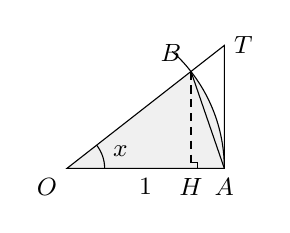
\begin{tikzpicture}[scale=2.0, font=\small]
\coordinate (O) at (0,0);
\coordinate (A) at (1,0);
\coordinate (B) at ({cos(38)},{sin(38)});
\coordinate (T) at (1,{tan(38)});
\coordinate (H) at ({cos(38)},0);
\fill[gray!12] (O)--(A) arc[start angle=0,end angle=38,radius=1]--cycle;
\draw (O)--(A)--(T)--cycle;
\draw (A)--(B);
\draw[densely dashed] (B)--(H);
\draw (H) ++(0,0.04)--++(0.04,0)--++(0,-0.04);
\draw (A) arc[start angle=0,end angle=48,radius=1];
\draw (0.24,0) arc[start angle=0,end angle=38,radius=0.24];
\node at (0.34,0.11) {$x$};
\node[below left] at (O) {$O$};
\node[below] at (A) {$A$};
\node[below] at (H) {$H$};
\node[above left] at (B) {$B$};
\node[right] at (T) {$T$};
\node[below] at (0.5,0) {$1$};
\end{tikzpicture}
\end{center}
作 $BH\perp OA$, 垂足为 $H$, 则 $BH=\sin x$. 下面比较三个图形的面积. $\triangle OAB$ 的底 $OA=1$, 高 $BH=\sin x$, 面积为 $\displaystyle\frac12\sin x$; 扇形 $OAB$ (图中阴影部分) 的半径为 $1$, 圆心角为 $x$, 面积为 $\displaystyle\frac12\cdot1^2\cdot x=\frac x2$; $\triangle OAT$ 的底 $OA=1$, 高 $AT=\tan x$, 面积为 $\displaystyle\frac12\tan x$.

$\triangle OAB$ 包含于扇形 $OAB$, 扇形又包含于 $\triangle OAT$. 扇形 $OAB$ 由 $\angle AOB$ 内与 $O$ 的距离不超过 $1$ 的点组成. $\triangle OAB$ 在 $\angle AOB$ 内, 它的每一点 $P$ 都在从 $O$ 到弦 $AB$ 上某一点 $Q$ 的线段上. $A$, $B$ 在圆周上, 而圆盘中两点的连线仍在圆盘中, 所以 $OQ\le1$, 从而 $OP\le OQ\le1$. 因此 $\triangle OAB$ 包含于扇形 $OAB$. $\triangle OAT$ 由 $\angle AOB$ 内横坐标不超过 $1$ 的点组成, 而扇形中的点的横坐标不超过它与 $O$ 的距离, 因而不超过 $1$, 所以扇形包含于 $\triangle OAT$. 扇形比 $\triangle OAB$ 多出弦 $AB$ 与弧 $AB$ 之间的弓形, $\triangle OAT$ 比扇形多出弧 $AB$ 与线段 $BT$、$TA$ 围成的部分, 这两块的面积都为正, 所以
\[
\frac12\sin x<\frac x2<\frac12\tan x,\qquad\text{即}\qquad\sin x<x<\tan x\quad\left(0<x<\frac\pi2\right).
\]
正弦是奇函数, 所以 $\displaystyle-\frac\pi2<x<0$ 时 $|\sin x|=\sin(-x)<-x=|x|$; 当 $\displaystyle|x|\ge\frac\pi2$ 时 $|\sin x|\le1<|x|$. 因此对一切 $x$ 都有 $|\sin x|\le|x|$.

由 $-|x|\le\sin x\le|x|$ 及两边夹定理, $\displaystyle\lim_{x\to0}\sin x=0$. 再由半角公式和复合函数的极限 (令 $\displaystyle u=\frac x2$),
\[
\lim_{x\to0}(1-\cos x)=\lim_{x\to0}2\sin^2\frac x2=2\left(\lim_{u\to0}\sin u\right)^2=0,
\]
所以 $\displaystyle\lim_{x\to0}\cos x=1$.
\end{cnproof}
任意一点 $c$ 处的极限可以由此得到. 令 $h=x-c$, 由复合函数的极限、和角公式及四则运算法则,
\[
\begin{aligned}
\lim_{x\to c}\sin x&=\lim_{h\to0}(\sin c\cos h+\cos c\sin h)=\sin c\cdot1+\cos c\cdot0=\sin c,\\
\lim_{x\to c}\cos x&=\lim_{h\to0}(\cos c\cos h-\sin c\sin h)=\cos c\cdot1-\sin c\cdot0=\cos c.
\end{aligned}
\]
\begin{theorem}[第一个重要极限]
$\displaystyle\lim_{x\to0}\frac{\sin x}x=1$.
\end{theorem}
由 $|\sin x|\le|x|$ 只知道比值的绝对值不超过 $1$, 看不出它趋于 $1$. 要用两边夹定理, 还需要一个同样趋于 $1$ 的下界. 本节例\ref{ex:6-5} 中的另一半不等式 $x<\tan x$ 可以化为 $\displaystyle\frac{\sin x}x>\cos x$, 这就是所要的下界.
\begin{cnproof}
当 $\displaystyle0<x<\frac\pi2$ 时, $\sin x>0$, $\cos x>0$. 由 $\sin x<x$ 得 $\displaystyle\frac{\sin x}x<1$; 由 $\displaystyle x<\frac{\sin x}{\cos x}$ 得 $\displaystyle\cos x<\frac{\sin x}x$. 所以
\[
\cos x<\frac{\sin x}x<1\qquad\left(0<x<\frac\pi2\right).
\]
由于 $\cos x$ 与 $\displaystyle\frac{\sin x}x$ 都是偶函数, 这个不等式在 $\displaystyle-\frac\pi2<x<0$ 时也成立. 由 $\displaystyle\lim_{x\to0}\cos x=1$ 及两边夹定理, $\displaystyle\lim_{x\to0}\frac{\sin x}x=1$.
\end{cnproof}
\begin{example}\label{ex:6-6}
\textnormal{(教材例6.6)} 求 $\displaystyle\lim_{x\to0}\frac{1-\cos x}{2x^2}$.
\end{example}
\par\indent\textbf{分析:} 分子、分母都趋于零. 已知的重要极限是 $\displaystyle\frac{\sin u}u$ 型的, 而分子中只有余弦, 所以先用半角公式把 $1-\cos x$ 化为 $\displaystyle2\sin^2\frac x2$. 正弦的自变量是 $\displaystyle\frac x2$, 所以分母也写成 $\displaystyle\left(\frac x2\right)^2$ 的倍数, 即 $\displaystyle2x^2=8\left(\frac x2\right)^2$, 配出的常数 $8$ 要保留.
\begin{cnsolution}
令 $\displaystyle u=\frac x2$, 由复合函数的极限及积的法则,
\[
\lim_{x\to0}\frac{1-\cos x}{2x^2}=\lim_{x\to0}\frac{2\sin^2\frac x2}{2x^2}=\lim_{x\to0}\frac14\left(\frac{\sin\frac x2}{\frac x2}\right)^2=\frac14\left(\lim_{u\to0}\frac{\sin u}u\right)^2=\frac14.
\]
\end{cnsolution}
由此得到以后常用的结果 $\displaystyle\lim_{x\to0}\frac{1-\cos x}{x^2}=\frac12$.
\begin{example}
\textnormal{(课堂例题: 第一个重要极限的基本变形)} 求
\[
\text{(1)}\ \lim_{x\to0}\frac x{\sin x};\qquad\text{(2)}\ \lim_{x\to\infty}x\sin\frac1x;\qquad\text{(3)}\ \lim_{x\to0}\frac{\tan x}x;\qquad\text{(4)}\ \lim_{x\to0}\frac{\sin2x}{\tan5x}.
\]
\end{example}
\par\indent\textbf{分析:} 使用第一个重要极限时, 正弦的自变量与分母必须是同一个趋于零的量. (1) 是 $\displaystyle\frac{\sin x}x$ 的倒数, 用商的法则. (2) 中趋于零的量是 $\displaystyle\frac1x$, 所以令 $\displaystyle t=\frac1x$. (3) 把正切写成正弦与余弦之比. (4) 中有两个不同的角 $2x$ 与 $5x$. 由 (3) 知 $\displaystyle\lim_{v\to0}\frac{\tan v}v=1$, 所以正切可以与正弦同样处理. 于是分子、分母按各自的角分别配出 $\displaystyle\frac{\sin2x}{2x}$ 与 $\displaystyle\frac{5x}{\tan5x}$:
\[
\frac{\sin2x}{\tan5x}=\frac{2x}{5x}\cdot\frac{\sin2x}{2x}\cdot\frac{5x}{\tan5x},
\]
配出的系数 $\displaystyle\frac{2x}{5x}=\frac25$ 保留下来.
\begin{cnsolution}
(1) 由商的法则,
\[
\lim_{x\to0}\frac x{\sin x}=\frac1{\displaystyle\lim_{x\to0}\frac{\sin x}x}=1.
\]

(2) 令 $\displaystyle t=\frac1x$, 则 $x\to\infty$ 时 $t\to0$, 且 $t\ne0$. 由复合函数的极限,
\[
\lim_{x\to\infty}x\sin\frac1x=\lim_{t\to0}\frac{\sin t}t=1.
\]

(3) 由 $\displaystyle\lim_{x\to0}\cos x=1\ne0$,
\[
\lim_{x\to0}\frac{\tan x}x=\lim_{x\to0}\left(\frac{\sin x}x\cdot\frac1{\cos x}\right)=1\cdot1=1.
\]

(4) 当 $\displaystyle0<|x|<\frac\pi{10}$ 时, $\tan5x$ 有定义且不为零. 令 $u=2x$, $v=5x$. 由复合函数的极限、(3) 及四则运算法则,
\[
\begin{aligned}
\lim_{x\to0}\frac{\sin2x}{\tan5x}
&=\lim_{x\to0}\left(\frac25\cdot\frac{\sin2x}{2x}\cdot\frac{5x}{\tan5x}\right)\\
&=\frac25\cdot\lim_{u\to0}\frac{\sin u}u\cdot\frac1{\displaystyle\lim_{v\to0}\frac{\tan v}v}=\frac25.
\end{aligned}
\]
\end{cnsolution}
\begin{example}
\textnormal{(课堂例题: 反三角函数的换元)} 求 $\displaystyle\lim_{x\to0}\frac{\arcsin x}x$ 及 $\displaystyle\lim_{x\to0}\frac{\arctan x}x$.
\end{example}
\par\indent\textbf{分析:} 已知的是三角函数的极限, 题中出现的却是反三角函数. 把反三角函数的值记为新的变量 $t$, 自变量就成为 $x=\sin t$ 或 $x=\tan t$, 式子化为 $\displaystyle\frac t{\sin t}$ 或 $\displaystyle\frac t{\tan t}$. 它们分别是 $\displaystyle\frac{\sin t}t$ 与 $\displaystyle\frac{\tan t}t$ 的倒数, 由第一个重要极限和 $\displaystyle\lim_{t\to0}\frac{\tan t}t=1$, 在 $t\to0$ 时都趋于 $1$. 换元要用复合函数的极限, 须先验证 $x\to0$ 时 $t\to0$, 并且 $x\ne0$ 时 $t\ne0$. 其中 $t\to0$ 由反三角函数的单调性得到. 若 $\displaystyle0<\eta<\frac\pi2$, 则 $\arcsin(\pm\sin\eta)=\pm\eta$. 由反正弦函数严格增加, $|x|<\sin\eta$ 时 $-\eta<\arcsin x<\eta$; 反正切的情形把 $\sin\eta$ 换成 $\tan\eta$. 任给的 $\varepsilon$ 未必小于 $\displaystyle\frac\pi2$, 所以取 $\displaystyle\eta=\min\left\{\varepsilon,\frac\pi4\right\}$.
\begin{cnsolution}
令 $t=\arcsin x$ ($|x|\le1$), 则 $x=\sin t$, $\displaystyle|t|\le\frac\pi2$. 先证 $x\to0$ 时 $t\to0$. 任给 $\varepsilon>0$, 令 $\displaystyle\eta=\min\left\{\varepsilon,\frac\pi4\right\}$, 取 $\delta=\sin\eta$. 当 $0<|x|<\delta$ 时, 由反正弦函数严格增加, $-\eta<\arcsin x<\eta$, 即 $|t|<\eta\le\varepsilon$. 又 $x\ne0$ 时 $t\ne0$. 由复合函数的极限及第一个重要极限,
\[
\lim_{x\to0}\frac{\arcsin x}x=\lim_{t\to0}\frac t{\sin t}=1.
\]
令 $t=\arctan x$, 则 $x=\tan t$. 对同样的 $\eta$, 当 $|x|<\tan\eta$ 时, 由反正切函数严格增加, $|t|<\eta\le\varepsilon$, 所以 $x\to0$ 时 $t\to0$; 又 $x\ne0$ 时 $t\ne0$. 由复合函数的极限及 $\displaystyle\lim_{t\to0}\frac{\tan t}t=1$,
\[
\lim_{x\to0}\frac{\arctan x}x=\lim_{t\to0}\frac t{\tan t}=\frac1{\displaystyle\lim_{t\to0}\frac{\tan t}t}=1.
\]
\end{cnsolution}
\begin{theorem}[第二个重要极限]
\[
\lim_{x\to\infty}\left(1+\frac1x\right)^x=e,\qquad\lim_{t\to0}(1+t)^{\frac1t}=e.
\]
\end{theorem}
\par\indent\textbf{分析:} 1.4 节把 $\displaystyle\left(1+\frac1n\right)^n$ 的极限定义为 $e$, 但那里 $n$ 只取正整数, 现在 $x$ 取一切实数. 要把实数 $x$ 与整数联系起来, 可以用相邻的两个整数夹住它. 令 $n=[x]$, 则 $n\le x<n+1$, 底数满足 $\displaystyle1+\frac1{n+1}<1+\frac1x\le1+\frac1n$. 指数为正时, 乘幂随底数增大而增大; 底数大于 $1$ 时, 乘幂随指数增大而增大. 每次只改变底数或只改变指数, 得
\[
\left(1+\frac1{n+1}\right)^n\le\left(1+\frac1{n+1}\right)^x\le\left(1+\frac1x\right)^x\le\left(1+\frac1n\right)^x\le\left(1+\frac1n\right)^{n+1}.
\]
左端是 $\displaystyle\left(1+\frac1{n+1}\right)^{n+1}$ 除以 $\displaystyle1+\frac1{n+1}$, 右端是 $\displaystyle\left(1+\frac1n\right)^n$ 乘以 $\displaystyle1+\frac1n$, 都趋于 $e$.

$x\to-\infty$ 时底数小于 $1$, 上面的单调关系不能照搬. 令 $y=-x$, 则
\[
\left(1+\frac1x\right)^x=\left(1-\frac1y\right)^{-y}=\left(\frac{y-1}y\right)^{-y}=\left(\frac y{y-1}\right)^y,
\]
底数 $\displaystyle\frac y{y-1}=1+\frac1{y-1}$ 又大于 $1$, 可以化为已证的情形.
\begin{cnproof}
先设 $x\to+\infty$, 只需考虑 $x\ge1$. 令 $n=[x]$, 则 $n\ge1$, $n\le x<n+1$, 从而 $\displaystyle1<1+\frac1{n+1}<1+\frac1x\le1+\frac1n$. 这里的底数都大于 $1$, 指数都是正数, 由乘幂关于底数和指数的单调性,
\[
\left(1+\frac1{n+1}\right)^n\le\left(1+\frac1x\right)^x\le\left(1+\frac1n\right)^{n+1}.
\]
记
\[
b_n=\left(1+\frac1{n+1}\right)^n=\frac{\left(1+\frac1{n+1}\right)^{n+1}}{1+\frac1{n+1}},\qquad c_n=\left(1+\frac1n\right)^{n+1}=\left(1+\frac1n\right)^n\left(1+\frac1n\right).
\]
由 1.4 节 $e$ 的定义、去掉首项不改变极限以及四则运算法则, $b_n\to e$, $c_n\to e$. 不等式的两端是 $b_{[x]}$ 与 $c_{[x]}$, 即这两个数列在 $n=[x]$ 处的值. 这里内层的 $[x]$ 无限增大, 外层又是数列, 复合函数的极限不能直接使用. 下面按定义验证它们当 $x\to+\infty$ 时的极限. 任给 $\varepsilon>0$, 存在 $N$, 使 $n>N$ 时 $|b_n-e|<\varepsilon$, $|c_n-e|<\varepsilon$. 当 $x>N+1$ 时 $[x]>x-1>N$, 因而
\[
e-\varepsilon<b_{[x]}\le\left(1+\frac1x\right)^x\le c_{[x]}<e+\varepsilon.
\]
所以 $\displaystyle\lim_{x\to+\infty}\left(1+\frac1x\right)^x=e$.

再设 $x\to-\infty$. 令 $y=-x$, 当 $x<-2$ 时 $y>2$, 并且
\[
\left(1+\frac1x\right)^x=\left(1-\frac1y\right)^{-y}=\left(\frac y{y-1}\right)^y=\left(1+\frac1{y-1}\right)^{y-1}\left(1+\frac1{y-1}\right).
\]
记
\[
F(u)=\left(1+\frac1u\right)^u\left(1+\frac1u\right).
\]
由已证的情形、$\displaystyle\lim_{u\to+\infty}\left(1+\frac1u\right)=1$ 及积的法则, $\displaystyle\lim_{u\to+\infty}F(u)=e$. 任给 $\varepsilon>0$, 存在 $A>0$, 使 $u>A$ 时 $|F(u)-e|<\varepsilon$. 当 $x<-(A+2)$ 时, $x<-2$, 并且 $u=y-1=-x-1>A+1>A$, 于是 $\displaystyle\left|\left(1+\frac1x\right)^x-e\right|=|F(u)-e|<\varepsilon$. 所以 $\displaystyle\lim_{x\to-\infty}\left(1+\frac1x\right)^x=e$. 两个方向的极限都是 $e$, 由 1.5 节定理1, 第一个等式成立.

最后证明第二个等式. 任给 $\varepsilon>0$, 由第一个等式, 存在 $A\ge1$, 使 $|x|>A$ 时 $\displaystyle\left|\left(1+\frac1x\right)^x-e\right|<\varepsilon$. 当 $\displaystyle0<|t|<\frac1A$ 时, $1+t>0$, 并且 $\displaystyle x=\frac1t$ 满足 $|x|>A$, 所以 $\bigl|(1+t)^{\frac1t}-e\bigr|<\varepsilon$.
\end{cnproof}
第二个重要极限中, 底数趋于 $1$ 而指数的绝对值无限增大, 这样的表达式俗称 $1^\infty$ 型. 它的极限取决于底数趋于 $1$ 和指数趋于无穷的相对快慢, 不能分别对底数和指数取极限. 例如先把底数换成它的极限 $1$, 就会误得 $\displaystyle\left(1+\frac1x\right)^x\to1$, 而实际的极限是 $e$. 底数和指数都含有自变量的函数称为幂指函数. 若它的底数和指数都有有限的极限, 并且底数的极限为正, 则可以分别取极限.
\begin{propositionsingle}[幂指函数的极限]
设 $\displaystyle\lim_{x\to a}u(x)=A$, $\displaystyle\lim_{x\to a}v(x)=B$, 且 $B>0$. 则 $\displaystyle\lim_{x\to a}v(x)^{u(x)}=B^A$.
\end{propositionsingle}
\begin{cnproof}
由保号性, $v(x)$ 在 $a$ 的某个去心邻域内为正, 可以写成 $v(x)^{u(x)}=e^{u(x)\ln v(x)}$. 由 1.5 节例\ref{ex:h15-3}, $\displaystyle\lim_{y\to B}\ln y=\ln B$, 即外层函数 $\ln y$ 在 $B$ 处的值等于它的极限. 由复合函数极限后面的说明, 这时不必要求 $v(x)\ne B$, 也有 $\ln v(x)\to\ln B$. 由积的法则, $u(x)\ln v(x)\to A\ln B$. 外层函数 $e^s$ 也满足 $\displaystyle\lim_{s\to s_0}e^s=e^{s_0}$ (本节例\ref{ex:6-3}), 同理得
\[
\lim_{x\to a}v(x)^{u(x)}=\lim_{x\to a}e^{u(x)\ln v(x)}=e^{A\ln B}=B^A.
\]
\end{cnproof}
命题对其他变化方式以及数列同样成立.

有了这个命题, 就可以借助第二个重要极限计算 $1^\infty$ 型的极限 $\displaystyle\lim(1+t)^w$, 其中 $t\to0$, $|w|$ 无限增大. 为此要凑出 $(1+t)^{\frac1t}$, 即把指数 $w$ 写成 $\displaystyle\frac1t$ 的倍数, 这个倍数只能是 $tw$:
\[
(1+t)^w=\left[(1+t)^{\frac1t}\right]^{tw}.
\]
方括号内的部分趋于 $e$. 若 $tw$ 趋于有限的数 $c$, 由幂指函数的极限, 整个表达式趋于 $e^c$. 计算时, 令 $t$ 等于底数减 $1$. 换元要求在所考察的范围内 $t\ne0$, 乘幂要求底数 $1+t>0$, 这两点都要检验.
\begin{example}\label{ex:6-7}
\textnormal{(教材例6.7)} 求 $\displaystyle\lim_{x\to\infty}\left(\frac{2x+1}{2x+3}\right)^x$.
\end{example}
\par\indent\textbf{分析:} 底数 $\displaystyle\frac{2x+1}{2x+3}\to1$, 指数 $x$ 的绝对值无限增大, 是 $1^\infty$ 型. 把底数写成 $1+t$, 原式就是 $\bigl[(1+t)^{\frac1t}\bigr]^{xt}$. 方括号内趋于 $e$, 所以只需求 $t$ 与指数 $x$ 的乘积 $xt$ 的极限.
\begin{cnsolution}
令 $\displaystyle t=\frac{2x+1}{2x+3}-1=\frac{(2x+1)-(2x+3)}{2x+3}=-\frac2{2x+3}$. 当 $x\to\infty$ 时 $t\to0$; 当 $|x|>3$ 时 $t\ne0$, 且 $\displaystyle1+t=\frac{2x+1}{2x+3}>0$. $t$ 与指数的乘积的极限为
\[
\lim_{x\to\infty}xt=\lim_{x\to\infty}\frac{-2x}{2x+3}=\lim_{x\to\infty}\frac{-2}{2+\frac3x}=-1.
\]
由第二个重要极限、复合函数的极限及幂指函数的极限,
\[
\lim_{x\to\infty}\left(\frac{2x+1}{2x+3}\right)^x=\lim_{x\to\infty}\left[(1+t)^{\frac1t}\right]^{xt}=e^{-1}.
\]
\end{cnsolution}
\begin{example}\label{ex:6-8}
\textnormal{(教材例6.8)} 设 $a>0$, $\mu\in\mathbb R$, 证明 $\displaystyle\lim_{x\to a}x^\mu=a^\mu$.
\end{example}
\begin{cnproof}
$\mu$ 是正整数时, 1.5 节例\ref{ex:5-2} 已经用因式分解证明. 一般的实数 $\mu$ 没有这样的因式分解. 但 $x^\mu$ 是幂指函数 $v(x)^{u(x)}$ 的特殊情形, 其底数 $v(x)=x$, 指数 $u(x)\equiv\mu$. 当 $x\to a$ 时, 底数趋于 $a>0$, 指数是常数 $\mu$. 由幂指函数的极限,
\[
\lim_{x\to a}x^\mu=a^\mu.
\]
\end{cnproof}
当 $\mu>0$ 时还有 $\displaystyle\lim_{x\to0^+}x^\mu=0$. 事实上, 任给 $\varepsilon>0$, 当 $0<x<\varepsilon^{\frac1\mu}$ 时, 由幂函数 $x^\mu$ 在 $(0,+\infty)$ 上严格增加, $0<x^\mu<\varepsilon$.
\subsection{运算法则与重要极限的应用}
\par\indent\textbf{方法小结:} 求函数极限, 先看自变量按指定方式变化时各部分怎样变化, 判断式子的类型. 各部分都有有限的极限, 并且分母的极限不为零时, 才能用四则运算法则把一个极限拆成几个极限的和、积、商. $\displaystyle\frac00$ 型要设法约去趋于零的公因子, 或者化出已知的极限: 有理分式先因式分解 (代入 $x=a$ 后某个多项式为零, 它就含有因子 $x-a$); 含根式时用平方差公式有理化; 含三角函数时用半角公式等三角恒等式化出 $\displaystyle\frac{\sin u}u$ 的形式. $\displaystyle\frac\infty\infty$ 型的分子、分母同除以起主要作用的项. $\infty-\infty$ 型先通分或有理化, 化成一个分式. 有界因子乘以趋于零的因子, 用两边夹定理. $1^\infty$ 型把底数写成 $1+t$, 利用 $(1+t)^w=\bigl[(1+t)^{\frac1t}\bigr]^{tw}$ 改求 $tw$ 的极限.

换元时要检验新变量的趋向, 并检验在所考察的范围内新变量不取它的极限值. 每一步变形都要在所考察的范围内有意义 (分母不为零、根式有意义、底数为正), 所以常常先写出一个满足这些要求的范围. 要说明极限不存在, 可以找两列点, 它们都趋于指定的点且各项都不等于该点, 而函数值的极限不同; 也可以说明左、右极限不相等.
\begin{example}
\textnormal{(指定作业: 习题1.6第1题(4))} 求 $\displaystyle\lim_{x\to\infty}\frac{x^2-1}{2x^2-x-1}$.
\end{example}
\begin{cnsolution}
分子、分母都无限增大, 同除以最高次幂 $x^2$ 后各项都有有限的极限, 分母的极限不为零:
\[
\lim_{x\to\infty}\frac{x^2-1}{2x^2-x-1}=\lim_{x\to\infty}\frac{1-\frac1{x^2}}{2-\frac1x-\frac1{x^2}}=\frac{1-0}{2-0-0}=\frac12.
\]
\end{cnsolution}
\begin{example}
\textnormal{(指定作业: 习题1.6第1题(5))} 求 $\displaystyle\lim_{x\to1}\left(\frac1{1-x}-\frac3{1-x^3}\right)$.
\end{example}
\begin{cnsolution}
与本节例\ref{ex:6-2} 同型, 先通分. 由 $1-x^3=(1-x)(1+x+x^2)$, 通分后的分子是 $x^2+x-2=(x-1)(x+2)$, 含有因子 $x-1$. 分母中的因子 $1-x$ 等于 $-(x-1)$, 所以在 $x\ne1$ 时约去 $x-1$, 会出现一个负号:
\[
\begin{aligned}
\lim_{x\to1}\left(\frac1{1-x}-\frac3{1-x^3}\right)
&=\lim_{x\to1}\frac{(1+x+x^2)-3}{(1-x)(1+x+x^2)}=\lim_{x\to1}\frac{(x-1)(x+2)}{-(x-1)(1+x+x^2)}\\
&=\lim_{x\to1}\frac{-(x+2)}{1+x+x^2}=-1.
\end{aligned}
\]
\end{cnsolution}
\begin{example}
\textnormal{(指定作业: 习题1.6第1题(6))} 求 $\displaystyle\lim_{x\to4}\frac{\sqrt{2x+1}-3}{\sqrt{x-2}-\sqrt2}$.
\end{example}
\begin{cnsolution}
代入 $x=4$ 时分子、分母都为零. 根式之差中看不出因子 $x-4$, 由平方差公式把两个根式之差分别有理化:
\[
\sqrt{2x+1}-3=\frac{2(x-4)}{\sqrt{2x+1}+3},\qquad\sqrt{x-2}-\sqrt2=\frac{x-4}{\sqrt{x-2}+\sqrt2},
\]
公因子 $x-4$ 就显露出来. 在 $4$ 的去心邻域 $\mathring U(4,2)$ 内 $x>2$, 各根式都有意义, 并且 $x-4\ne0$, 于是
\[
\begin{aligned}
\lim_{x\to4}\frac{\sqrt{2x+1}-3}{\sqrt{x-2}-\sqrt2}
&=\lim_{x\to4}\left(\frac{2(x-4)}{\sqrt{2x+1}+3}\cdot\frac{\sqrt{x-2}+\sqrt2}{x-4}\right)\\
&=\lim_{x\to4}\frac{2\left(\sqrt{x-2}+\sqrt2\right)}{\sqrt{2x+1}+3}=\frac{2\cdot2\sqrt2}{3+3}=\frac{2\sqrt2}3,
\end{aligned}
\]
其中根式的极限由本节例\ref{ex:k16-1} 得到.
\end{cnsolution}
\begin{example}
\textnormal{(指定作业: 习题1.6第2题(4))} 求 $\displaystyle\lim_{x\to a}\frac{\sin x-\sin a}{x-a}$.
\end{example}
\begin{cnsolution}
分子是两个正弦之差, 分母是自变量之差, 两者都趋于零. 用和差化积把分子变成乘积 $\displaystyle2\cos\frac{x+a}2\sin\frac{x-a}2$, 其中正弦的自变量 $\displaystyle\frac{x-a}2$ 与分母只差一个常数倍. 令 $\displaystyle u=\frac{x-a}2$, 则 $x\to a$ 时 $u\to0$, $u\ne0$, 于是
\[
\lim_{x\to a}\frac{\sin x-\sin a}{x-a}=\lim_{x\to a}\left(\cos\frac{x+a}2\cdot\frac{\sin\frac{x-a}2}{\frac{x-a}2}\right)=\lim_{x\to a}\cos\frac{x+a}2\cdot\lim_{u\to0}\frac{\sin u}u=\cos a.
\]
余弦因子的极限由任意点处余弦的极限及复合函数极限后面的说明得到.
\end{cnsolution}
\begin{example}
\textnormal{(指定作业: 习题1.6第2题(6))} 求 $\displaystyle\lim_{x\to0}\frac{\tan x-\sin x}{\sin^3x}$.
\end{example}
\par\indent\textbf{分析:} 分子、分母都趋于零. 若把分式拆成 $\displaystyle\frac{\tan x}{\sin^3x}$ 与 $\displaystyle\frac{\sin x}{\sin^3x}$ 之差, 两项都没有有限的极限, 不能用差的法则, 所以先化简分子. 把正切写成 $\displaystyle\frac{\sin x}{\cos x}$, 分子成为 $\displaystyle\frac{\sin x(1-\cos x)}{\cos x}$, 可与分母约去 $\sin x$; 分母剩下的 $\sin^2x$ 写成 $(1-\cos x)(1+\cos x)$, 又可以约去 $1-\cos x$.
\begin{cnsolution}
在 $0$ 的充分小的去心邻域内 $\sin x\ne0$, $\cos x\ne0$, 由 $\sin^2x=(1-\cos x)(1+\cos x)$ 也有 $1-\cos x\ne0$, 于是
\[
\begin{aligned}
\lim_{x\to0}\frac{\tan x-\sin x}{\sin^3x}
&=\lim_{x\to0}\frac{\sin x(1-\cos x)}{\cos x\sin^3x}=\lim_{x\to0}\frac{1-\cos x}{\cos x(1-\cos x)(1+\cos x)}\\
&=\lim_{x\to0}\frac1{\cos x(1+\cos x)}=\frac1{1\cdot2}=\frac12.
\end{aligned}
\]
\end{cnsolution}
\begin{example}
\textnormal{(指定作业: 习题1.6第2题(8))} 求 $\displaystyle\lim_{x\to0}\frac{\sqrt{1-\cos x}}x$.
\end{example}
\begin{cnsolution}
由半角公式, $\displaystyle\sqrt{1-\cos x}=\sqrt2\left|\sin\frac x2\right|$, 开方后出现绝对值, 而分母 $x$ 带有符号, 所以分左、右两侧计算. 当 $0<x<\pi$ 时 $\displaystyle\sin\frac x2>0$, 令 $\displaystyle u=\frac x2$,
\[
\lim_{x\to0^+}\frac{\sqrt{1-\cos x}}x=\lim_{x\to0^+}\frac{\sqrt2\sin\frac x2}x=\frac{\sqrt2}2\lim_{u\to0^+}\frac{\sin u}u=\frac{\sqrt2}2.
\]
当 $-\pi<x<0$ 时 $\displaystyle\left|\sin\frac x2\right|=-\sin\frac x2$, 同理左极限为 $\displaystyle-\frac{\sqrt2}2$. 左、右极限不相等, 所求极限不存在.
\end{cnsolution}
\begin{example}
\textnormal{(指定作业: 习题1.6第2题(10))} 求 $\displaystyle\lim_{x\to0}(1-\tan x)^{\frac1{\sin x}}$.
\end{example}
\begin{cnsolution}
底数趋于 $1$, 指数的绝对值无限增大. 令 $t=-\tan x$, 则 $x\to0$ 时 $t\to0$; 在 $0$ 的充分小的去心邻域内 $t\ne0$, $1+t>0$. $t$ 与指数的乘积的极限为
\[
\lim_{x\to0}\frac t{\sin x}=\lim_{x\to0}\frac{-\tan x}{\sin x}=\lim_{x\to0}\frac{-1}{\cos x}=-1,
\]
所以
\[
\lim_{x\to0}(1-\tan x)^{\frac1{\sin x}}=\lim_{x\to0}\left[(1+t)^{\frac1t}\right]^{\frac t{\sin x}}=e^{-1}.
\]
\end{cnsolution}
\begin{example}
\textnormal{(指定作业: 习题1.6第2题(11))} 求 $\displaystyle\lim_{x\to\infty}\left(\frac{2x-1}{2x+1}\right)^x$.
\end{example}
\begin{cnsolution}
与本节例\ref{ex:6-7} 同型. 令 $\displaystyle t=\frac{2x-1}{2x+1}-1=\frac{(2x-1)-(2x+1)}{2x+1}=-\frac2{2x+1}$, 则 $x\to\infty$ 时 $t\to0$; 当 $|x|>2$ 时 $t\ne0$, $1+t>0$. 由
\[
\lim_{x\to\infty}xt=\lim_{x\to\infty}\frac{-2x}{2x+1}=\lim_{x\to\infty}\frac{-2}{2+\frac1x}=-1,
\]
得
\[
\lim_{x\to\infty}\left(\frac{2x-1}{2x+1}\right)^x=\lim_{x\to\infty}\left[(1+t)^{\frac1t}\right]^{xt}=e^{-1}.
\]
\end{cnsolution}
\begin{example}
\textnormal{(指定作业: 习题1.6第2题(13))} 对固定的实数 $x$, 求 $\displaystyle\lim_{n\to\infty}\left(1+\frac xn+\frac{x^2}{2n^2}\right)^{-n}$.
\end{example}
\begin{cnsolution}
这里变化的是 $n$, $x$ 是固定的参数. 底数趋于 $1$, 指数 $-n$ 的绝对值无限增大. 若 $x=0$, 各项都是 $1$, 极限为 $1$. 设 $x\ne0$, 令 $\displaystyle t_n=\frac xn+\frac{x^2}{2n^2}=\frac{2nx+x^2}{2n^2}$, 则 $t_n\to0$; 当 $\displaystyle n>\frac{|x|}2$ 时 $2n+x>0$, 所以 $2nx+x^2=x(2n+x)\ne0$, $t_n\ne0$. 底数
\[
1+t_n=\frac12\left(2+\frac{2x}n+\frac{x^2}{n^2}\right)=\frac12\left[\left(1+\frac xn\right)^2+1\right]>0.
\]
$t_n$ 与指数的乘积的极限为
\[
\lim_{n\to\infty}(-nt_n)=\lim_{n\to\infty}\left(-x-\frac{x^2}{2n}\right)=-x,
\]
其中 $t_n$ 的第二项 $\displaystyle\frac{x^2}{2n^2}$ 乘以 $n$ 后趋于零, 对结果没有影响. 但这一点要在算出 $-nt_n$ 以后才能看出, 写 $t_n$ 时不能事先把它丢掉. 由海涅定理, $\displaystyle(1+t_n)^{\frac1{t_n}}\to e$, 再由数列情形的幂指函数的极限,
\[
\lim_{n\to\infty}\left(1+\frac xn+\frac{x^2}{2n^2}\right)^{-n}=\lim_{n\to\infty}\left[(1+t_n)^{\frac1{t_n}}\right]^{-nt_n}=e^{-x}.
\]
$x=0$ 时结果 $1=e^0$ 也符合这个公式.
\end{cnsolution}
\begin{example}
\textnormal{(指定作业: 习题1.6第2题(14))} 求 $\displaystyle\lim_{x\to0}(\cos x)^{\frac1{x^2}}$.
\end{example}
\begin{cnsolution}
底数趋于 $1$, 指数无限增大. 令 $t=\cos x-1$, 则 $x\to0$ 时 $t\to0$; 在 $\displaystyle\mathring U\left(0,\frac\pi2\right)$ 内 $t\ne0$, $1+t=\cos x>0$. 由本节例\ref{ex:6-6} 后的结果,
\[
\lim_{x\to0}\frac t{x^2}=-\lim_{x\to0}\frac{1-\cos x}{x^2}=-\frac12,
\]
所以
\[
\lim_{x\to0}(\cos x)^{\frac1{x^2}}=\lim_{x\to0}\left[(1+t)^{\frac1t}\right]^{\frac t{x^2}}=e^{-\frac12}.
\]
\end{cnsolution}
\begin{example}
\textnormal{(指定作业: 习题1.6第6题)} 已知 $\displaystyle\lim_{x\to\infty}\left(\frac{x+a}{x-a}\right)^x=9$, 求常数 $a$.
\end{example}
\begin{cnsolution}
先把含参数 $a$ 的极限算出来, 再令它等于 $9$. 若 $a=0$, 表达式恒为 $1$, 极限为 $1\ne9$, 不合题意. 设 $a\ne0$, 令 $\displaystyle t=\frac{x+a}{x-a}-1=\frac{2a}{x-a}$, 则 $x\to\infty$ 时 $t\to0$; 当 $|x|>3|a|$ 时 $t\ne0$, 并且 $|x-a|\ge|x|-|a|>2|a|$, 所以 $|t|<1$, $1+t>0$. 由
\[
\lim_{x\to\infty}xt=\lim_{x\to\infty}\frac{2ax}{x-a}=\lim_{x\to\infty}\frac{2a}{1-\frac ax}=2a,
\]
得
\[
\lim_{x\to\infty}\left(\frac{x+a}{x-a}\right)^x=\lim_{x\to\infty}\left[(1+t)^{\frac1t}\right]^{xt}=e^{2a}.
\]
由 $e^{2a}=9$ 得 $2a=\ln9$, 即 $a=\ln3$.
\end{cnsolution}
\section{无穷小和无穷大}
前面关心的是变量趋于什么值, 本节比较变量趋于零或趋于无穷的快慢. 两个量都趋于零时, 它们之差的极限总是零, 由此看不出哪个量趋于零更快; 比较快慢要看它们的比值. 这种比较能找出表达式中起主要作用的部分, 从而简化极限的计算.
\subsection{无穷小}
\begin{definition}
在某一极限过程中以 $0$ 为极限的函数, 称为这一过程中的\textbf{无穷小量}, 简称\textbf{无穷小}. 以 $0$ 为极限的数列也称为无穷小.
\end{definition}
无穷小是一个变量, 不是一个很小的数. 非零常数 $c$ 的绝对值无论多么小, 它的极限 $c$ 都不为零, 所以不是无穷小; 常数 $0$ 则是无穷小. 同一个函数在不同的过程中情况可能不同, 例如 $x$ 在 $x\to0$ 时是无穷小, 在 $x\to1$ 时不是. 所以说到无穷小, 必须指明极限过程.
\begin{example}
\textnormal{(教材例7.1)} 说明当 $x\to a$ 时 $(x-a)^2$ 与 $\sin(x-a)$ 是无穷小, 当 $x\to\infty$ 时 $\displaystyle\frac1x$、$\displaystyle\frac1{3x}$ 与 $\displaystyle\frac{x^2+x+1}{x^3+2}$ 是无穷小.
\end{example}
\begin{cnsolution}
只需验证各量在指定过程中的极限为零. 令 $h=x-a$, 当 $x\to a$ 时 $h\to0$, 所以 $(x-a)^2=h^2\to0$, $\sin(x-a)=\sin h\to0$. 当 $x\to\infty$ 时 $\displaystyle\frac1x\to0$, $\displaystyle\frac1{3x}=\frac13\cdot\frac1x\to0$. 最后一个量的分母次数高于分子, 同除以 $x^3$ 得
\[
\lim_{x\to\infty}\frac{x^2+x+1}{x^3+2}=\lim_{x\to\infty}\frac{\frac1x+\frac1{x^2}+\frac1{x^3}}{1+\frac2{x^3}}=\frac01=0.
\]
\end{cnsolution}
\begin{theoremsingle}
在同一极限过程中, $f\to L$ 的充分必要条件是 $f=L+\alpha$, 其中 $\alpha$ 是这一过程中的无穷小.
\end{theoremsingle}
\begin{cnproof}
若 $f\to L$, 令 $\alpha=f-L$, 由差的法则 $\alpha\to0$. 反过来, 若 $f=L+\alpha$, $\alpha\to0$, 由和的法则 $f\to L$.
\end{cnproof}
定理把“有极限”改写成“极限值加上一个无穷小”. 用 $L$ 近似代替 $f$ 时, 误差就是这个无穷小 $\alpha$, 它趋于零的快慢要用本节后面讲的无穷小的比较来描述.
\begin{proposition}
在同一极限过程中, 有限个无穷小之和是无穷小; 无穷小与局部有界的函数之积是无穷小. 特别地, 有限个无穷小之积是无穷小.
\end{proposition}
\begin{cnproof}
有限个无穷小之和由和的法则得到. 以 $x\to a$ 为例. 设 $\alpha\to0$, 而在 $\mathring U(a,\delta_0)$ 内 $|\beta|\le M$, $M>0$. 任给 $\varepsilon>0$, 存在 $\delta\in(0,\delta_0]$, 使 $0<|x-a|<\delta$ 时 $\displaystyle|\alpha|<\frac\varepsilon M$, 于是 $|\alpha\beta|\le M|\alpha|<\varepsilon$, 所以 $\alpha\beta\to0$. 无穷小有极限, 由局部有界性, 它在相应的范围内有界, 所以两个无穷小之积是无穷小.
\end{cnproof}
命题1 中的“有限个”不能去掉. 例如对每个固定的 $k$, $\displaystyle\frac k{n^2}$ 都是无穷小, 但项数随 $n$ 增加的和 $\displaystyle\frac1{n^2}+\frac2{n^2}+\cdots+\frac n{n^2}=\frac{n+1}{2n}\to\frac12$ (1.3 节运算法则后面的例子). 两个无穷小之商也没有确定的结论, 如 $x\to0$ 时, $\displaystyle\frac{x^2}x\to0$, $\displaystyle\frac{2x}x=2$, 而 $\displaystyle\frac x{x^2}=\frac1x$ 没有有限的极限.
\subsection{无穷大}
\begin{definition}
以 $x\to a$ 为例. 若对任意 $M>0$, 都存在 $\delta>0$, 使 $0<|x-a|<\delta$ 时恒有 $|f(x)|>M$, 则称当 $x\to a$ 时 $f(x)$ 为\textbf{无穷大量}, 简称\textbf{无穷大}, 记作 $\displaystyle\lim_{x\to a}f(x)=\infty$ 或 $f(x)\to\infty$ ($x\to a$). 若把条件 $|f(x)|>M$ 换成 $f(x)>M$ 或 $f(x)<-M$, 则分别称为\textbf{正无穷大}或\textbf{负无穷大}, 记作 $f(x)\to+\infty$ 或 $f(x)\to-\infty$. 其他极限过程以及数列的情形, 只需把去心邻域换成相应的范围.
\end{definition}
$\infty$ 不是实数. 写 $\displaystyle\lim_{x\to a}f(x)=\infty$ 时, 极限并不存在, 这个记号只描述 $|f(x)|$ 无限增大的情况, 不要求函数值在 $a$ 附近同号. 例如当 $x\to0$ 时 $\displaystyle\frac1x$ 是无穷大, 但它在 $0$ 的左侧为负, 右侧为正. 定义要求去心邻域 $0<|x-a|<\delta$ 内的\textbf{每一点}都满足 $|f(x)|>M$. 如果只知道 $a$ 附近有一些点处 $|f(x)|$ 可以任意大, 只能说明 $f$ 在 $a$ 附近无界, 不能说明它是无穷大.
\begin{example}
\textnormal{(指定作业: 习题1.7第3题)} 函数 $f(x)=x\cos x$ 在 $\mathbb R$ 上是否有界? 当 $x\to\infty$ 时是否为无穷大?
\end{example}
\begin{cnsolution}
在余弦取 $1$ 的点处, $|f(x)|=|x|$ 可以任意大; 在余弦的零点处, $f(x)=0$. 这两类点在任意远处都有. 取 $x_n=2n\pi$ ($n\in\mathbb N^+$), 则 $f(x_n)=2n\pi$, 可以超过任何正数, 所以 $f$ 在 $\mathbb R$ 上无界. “$x\to\infty$ 时 $f$ 是无穷大”是指对任意 $M>0$, 都存在 $A>0$, 使 $|x|>A$ 时恒有 $|f(x)|>M$. 把其中的量词依次否定, 就得到“$x\to\infty$ 时 $f$ 不是无穷大”的准确表述: 存在 $M>0$, 使对每个 $A>0$, 都有某个 $x$ 满足 $|x|>A$ 且 $|f(x)|\le M$. 取 $M=1$, $\displaystyle y_n=n\pi+\frac\pi2$ ($n\in\mathbb N^+$), 则 $f(y_n)=0$. 对任意 $A>0$, 由阿基米德性质, 存在 $n$ 使 $y_n>A$, 并且 $|f(y_n)|=0<M$, 所以 $f$ 不是无穷大. 故 $f$ 无界, 但当 $x\to\infty$ 时不是无穷大.
\end{cnsolution}
\begin{example}
\textnormal{(教材例7.2)} 用定义证明 $\displaystyle\lim_{x\to1}\frac{x+2}{x^2-1}=\infty$.
\end{example}
\par\indent\textbf{分析:} 要对任意 $M>0$ 找出 $\delta>0$, 使 $0<|x-1|<\delta$ 时 $\displaystyle\left|\frac{x+2}{x^2-1}\right|>M$. 分母趋于零, 分子趋于 $3$, 商的绝对值应当无限增大. 把分母分解为 $(x-1)(x+1)$, 原式的绝对值是
\[
\left|\frac{x+2}{x+1}\right|\cdot\frac1{|x-1|}.
\]
后一个因子在 $x\to1$ 时无限增大, 前一个因子趋于 $\displaystyle\frac32$. 要使原式的绝对值大于 $M$, 可以先把它缩小成一个较简单的式子, 再让这个式子大于 $M$. 后一个因子为正, 只要前一个因子在 $1$ 附近有正的下界 $m$, 原式的绝对值就不小于 $\displaystyle\frac m{|x-1|}$, 而 $\displaystyle\frac m{|x-1|}$ 随 $x\to1$ 无限增大. 为了得到 $m$, 先把 $x$ 限制在 $1$ 附近, 使 $x+1>0$. 只要半径不超过 $2$ 就可以, 这里取 $\displaystyle\frac12$. 当 $\displaystyle|x-1|<\frac12$ 时, $x+2>x+1>0$, 所以 $\displaystyle\frac{x+2}{x+1}>1$, 原式的绝对值大于 $\displaystyle\frac1{|x-1|}$. 剩下只需 $\displaystyle\frac1{|x-1|}>M$, 即 $\displaystyle|x-1|<\frac1M$.
\begin{cnproof}
当 $\displaystyle0<|x-1|<\frac12$ 时, $\displaystyle x>\frac12$, 所以 $x+2>x+1>0$,
\[
\left|\frac{x+2}{x^2-1}\right|=\frac{x+2}{x+1}\cdot\frac1{|x-1|}>\frac1{|x-1|}.
\]
任给 $M>0$, 取 $\displaystyle\delta=\min\left\{\frac12,\frac1M\right\}$. 当 $0<|x-1|<\delta$ 时, $\displaystyle\left|\frac{x+2}{x^2-1}\right|>\frac1{|x-1|}>M$. 故 $\displaystyle\lim_{x\to1}\frac{x+2}{x^2-1}=\infty$.
\end{cnproof}
当 $\displaystyle0<|x-1|<\frac12$ 时 $\displaystyle\frac{x+2}{x+1}>0$, 原式的符号与 $x-1$ 相同, 所以 $x\to1^-$ 时它是负无穷大, $x\to1^+$ 时它是正无穷大. 因此 $x\to1$ 时只能写 $\infty$, 不能写 $+\infty$ 或 $-\infty$.
\begin{proposition}
在同一极限过程中: 若 $\alpha\to0$ 且 $\alpha$ 在所考察的范围内不为零, 则 $\displaystyle\frac1\alpha\to\infty$; 若 $f\to\infty$, 则 $\displaystyle\frac1f\to0$. 两个无穷大之积是无穷大; 无穷大与局部有界的函数之和是无穷大. 若 $g\to c\ne0$, $\alpha\to0$, 且 $\alpha$ 在所考察的范围内不为零, 则 $\displaystyle\frac g\alpha\to\infty$; 如果 $\alpha$ 在这个范围内与 $c$ 同号, 则 $\displaystyle\frac g\alpha\to+\infty$, 如果异号, 则 $\displaystyle\frac g\alpha\to-\infty$.
\end{proposition}
\begin{cnproof}
任给 $M>0$, 由 $\alpha\to0$, 在相应范围内 $\displaystyle0<|\alpha|<\frac1M$, 即 $\displaystyle\left|\frac1\alpha\right|>M$. 任给 $\varepsilon>0$, 由 $f\to\infty$, 在相应范围内 $\displaystyle|f|>\frac1\varepsilon$, 即 $\displaystyle\left|\frac1f\right|<\varepsilon$.

若 $f,g$ 都是无穷大, 任给 $M>0$, 在相应范围内两者的绝对值都大于 $\sqrt M$, 于是 $|fg|>M$. 若 $f\to\infty$ 而 $|g|\le C$, 任给 $M>0$, 在相应范围内 $|f|>M+C$, 由反三角不等式 $|f+g|\ge|f|-|g|>M$.

最后, 设 $g\to c\ne0$. 由保号性, 在相应范围内 $g$ 与 $c$ 同号且 $\displaystyle|g|>\frac{|c|}2$. 任给 $M>0$, 由已证的 $\displaystyle\frac1\alpha\to\infty$, 在相应范围内 $\displaystyle\left|\frac1\alpha\right|>\frac{2M}{|c|}$, 于是 $\displaystyle\left|\frac g\alpha\right|=|g|\left|\frac1\alpha\right|>\frac{|c|}2\cdot\frac{2M}{|c|}=M$. 因为 $g$ 与 $c$ 同号, 所以 $\alpha$ 与 $c$ 同号时 $\displaystyle\frac g\alpha$ 为正, 从而大于 $M$; 异号时 $\displaystyle\frac g\alpha$ 为负, 从而小于 $-M$.
\end{cnproof}
两个无穷大之和、无穷大与无穷小之积都没有确定的结论. 例如当 $x\to+\infty$ 时, $x$ 与 $-x$ 都是无穷大, 和为 $0$; 而 $\displaystyle x\cdot\frac1{x^2}\to0$, $\displaystyle x\cdot\frac1x=1$, $\displaystyle x\cdot\frac1{\sqrt x}=\sqrt x\to+\infty$. 这类情形要具体计算.
\subsection{无穷小的比较}
设 $x\to0$. $x$ 与 $x^2$ 都是无穷小, $x$ 与 $2x$ 也都是无穷小. 但 $x^2$ 趋于零比 $x$ 快得多. 例如 $x=0.01$ 时 $x^2=0.0001$, 只是 $x$ 的百分之一; 一般地, $x^2$ 与 $x$ 之比等于 $x$, 随 $x$ 一起趋于零. $2x$ 则始终是 $x$ 的两倍. 要描述这种相对大小, 应以一个量为尺度, 看另一个量是它的多少倍, 也就是考察比值的极限. 1.6 节求过的 $\displaystyle\lim_{x\to0}\frac{\sin x}x=1$ 与 $\displaystyle\lim_{x\to0}\frac{1-\cos x}{x^2}=\frac12$ 都是这样的比值的极限.
\begin{definition}
设在同一极限过程中 $\alpha,\beta$ 都是无穷小, 且 $\beta$ 在所考察的范围内不为零.

\textup{(1)} 若 $\displaystyle\frac\alpha\beta\to0$, 则称 $\alpha$ 是比 $\beta$ \textbf{高阶的无穷小}, 记作 $\alpha=o(\beta)$.

\textup{(2)} 若 $\displaystyle\frac\alpha\beta\to k$, $k$ 是非零常数, 则称 $\alpha$ 与 $\beta$ 是\textbf{同阶无穷小}; 特别地, 若 $k=1$, 则称 $\alpha$ 与 $\beta$ 是\textbf{等价无穷小}, 记作 $\alpha\sim\beta$.

\textup{(3)} 若 $\displaystyle\left|\frac\alpha\beta\right|\to+\infty$, 则称 $\alpha$ 是比 $\beta$ \textbf{低阶的无穷小}.
\end{definition}
例如当 $x\to0$ 时 $x^2=o(x)$, $2x$ 与 $x$ 同阶但不等价, $\sin x\sim x$. 比值的极限也可能不存在, 如 $x\to0$ 时 $\displaystyle\frac{x\sin\frac1x}x=\sin\frac1x$, 这时两个量不能这样比较.

记号 $o(\beta)$ 表示某一个比 $\beta$ 高阶的无穷小, 它不是一个确定的函数. 例如 $x\to0$ 时 $x^2$ 与 $x^3$ 都可以记作 $o(x)$, 而 $x^2-x^3\ne0$, 所以 $o(\beta)-o(\beta)$ 未必等于 $0$. 另外约定 $o(1)$ 表示无穷小, 即与常数 $1$ 之比趋于零的量. 教材把同阶关系记作 $\alpha=O(\beta)$, 本书沿用这一记法. 不少书中的 $\alpha=O(\beta)$ 只要求比值 $\displaystyle\frac\alpha\beta$ 有界, 比同阶的要求低.

要说明一个无穷小趋于零有多快, 通常取一个简单的无穷小作为比较的尺度, 如 $x\to0$ 时取 $x$, $x\to a$ 时取 $x-a$, $x\to\infty$ 时取 $\displaystyle\frac1x$.
\begin{definition}
设 $\beta$ 是同一过程中取作尺度的无穷小, 在所考察的范围内不为零, $\mu>0$, 并且 $\beta^\mu$ 有意义 (例如 $\beta>0$, 或 $\mu$ 是正整数). 若 $\displaystyle\frac\alpha{\beta^\mu}\to k$, $k$ 是非零常数, 则称 $\alpha$ 是关于 $\beta$ 的 \textbf{$\mu$ 阶无穷小}, 并称 $k\beta^\mu$ 为 $\alpha$ 的\textbf{主部}.
\end{definition}
尺度相同时, 阶数越高, 趋于零越快. 若 $\alpha$, $\gamma$ 关于 $\beta$ 分别是 $\mu$ 阶与 $\nu$ 阶无穷小, $\nu>\mu$, 则 $\displaystyle\frac\gamma\alpha=\frac\gamma{\beta^\nu}\cdot\frac{\beta^\mu}\alpha\cdot\beta^{\nu-\mu}$, 右边前两个因子趋于非零常数, 第三个因子趋于零, 所以 $\gamma=o(\alpha)$.

由定义, $k\beta^\mu$ 是 $\alpha$ 的主部当且仅当 $\alpha\sim k\beta^\mu$. 这时 $\displaystyle\frac{\alpha-k\beta^\mu}{\beta^\mu}=\frac\alpha{\beta^\mu}-k\to0$, 即 $\alpha$ 与主部之差是比 $\beta^\mu$ 高阶的无穷小, 所以主部是 $\alpha$ 中起主要作用的部分, 同时反映 $\alpha$ 的大小和符号. 例如主部为 $-2x^3$ 表示 $\displaystyle\frac\alpha{x^3}\to-2$, 即 $\displaystyle\frac\alpha{-2x^3}\to1$; 由保号性, $x$ 接近 $0$ 时 $\alpha$ 与 $-2x^3$ 同号.
\begin{proposition}
在同一极限过程中, 设所涉及的无穷小在所考察的范围内都不为零.

\textup{(1)} $\alpha\sim\beta$ 的充分必要条件是 $\alpha=\beta+o(\beta)$.

\textup{(2)} 若 $\alpha\sim\beta$, 则 $\beta\sim\alpha$; 若 $\alpha\sim\beta$, $\beta\sim\gamma$, 则 $\alpha\sim\gamma$.

\textup{(3)} (等价替换) 设 $\alpha\sim\widetilde\alpha$, $f$ 是同一过程中的函数. 若 $\widetilde\alpha f$ 的极限存在或为 $\infty$, 则 $\alpha f$ 的极限也存在或为 $\infty$, 并且与前者相同; 若 $\displaystyle\frac f{\widetilde\alpha}$ 的极限存在或为 $\infty$, 则 $\displaystyle\frac f\alpha$ 也是如此. 因此乘积或商中的无穷小因子都可以换成与它等价的无穷小, 几个因子可以逐个替换.

\textup{(4)} 若 $\alpha\sim\widetilde\alpha$, $\beta\sim\widetilde\beta$, 且 $\displaystyle\frac{\widetilde\alpha}{\widetilde\beta}\to c$, $c\ne-1$, 则 $\alpha+\beta\sim\widetilde\alpha+\widetilde\beta$.
\end{proposition}
\begin{cnproof}
(1) 以 $\beta$ 为尺度衡量差 $\alpha-\beta$. 因为 $\displaystyle\frac{\alpha-\beta}\beta=\frac\alpha\beta-1$, 所以 $\displaystyle\frac\alpha\beta\to1$ 当且仅当 $\displaystyle\frac{\alpha-\beta}\beta\to0$, 即 $\alpha-\beta=o(\beta)$.

(2) 若 $\displaystyle\frac\alpha\beta\to1$, 由商的法则 $\displaystyle\frac\beta\alpha\to1$. 若还有 $\displaystyle\frac\beta\gamma\to1$, 则 $\displaystyle\frac\alpha\gamma=\frac\alpha\beta\cdot\frac\beta\gamma\to1$.

(3) 由定义及商的法则, $\displaystyle\frac\alpha{\widetilde\alpha}\to1$, $\displaystyle\frac{\widetilde\alpha}\alpha\to1$. 把替换前的表达式写成替换后的表达式乘以一个趋于 $1$ 的因子:
\[
\alpha f=\frac\alpha{\widetilde\alpha}\cdot\widetilde\alpha f,\qquad\frac f\alpha=\frac{\widetilde\alpha}\alpha\cdot\frac f{\widetilde\alpha}.
\]
若第二个因子有有限的极限 $c$, 由积的法则, 乘积也趋于 $c$. 若第二个因子是无穷大, 由保号性, 第一个因子在相应范围内大于 $\displaystyle\frac12$, 于是乘积的绝对值大于第二个因子的绝对值的一半, 乘积也是无穷大. 又因为第一个因子为正, 乘积与第二个因子同号, 所以正无穷大、负无穷大的情形也成立.

(4) 由 $c+1\ne0$ 及保号性, 在相应范围内 $\displaystyle\frac{\widetilde\alpha}{\widetilde\beta}+1\ne0$, 从而 $\widetilde\alpha+\widetilde\beta\ne0$. 分子、分母同除以 $\widetilde\beta$, 并把 $\displaystyle\frac\alpha{\widetilde\beta}$ 写成 $\displaystyle\frac\alpha{\widetilde\alpha}\cdot\frac{\widetilde\alpha}{\widetilde\beta}$, 得
\[
\frac{\alpha+\beta}{\widetilde\alpha+\widetilde\beta}=\frac{\frac\alpha{\widetilde\alpha}\cdot\frac{\widetilde\alpha}{\widetilde\beta}+\frac\beta{\widetilde\beta}}{\frac{\widetilde\alpha}{\widetilde\beta}+1}\to\frac{1\cdot c+1}{c+1}=1.
\]
\end{cnproof}
由 (2) 知 $\widetilde\alpha\sim\alpha$, 所以 (3) 中 $\alpha$ 与 $\widetilde\alpha$ 的地位可以互换, 替换前后两个式子的极限同时存在或同时不存在, 计算时可以直接写等式链. (3) 的证明只用到 $\displaystyle\frac\alpha{\widetilde\alpha}\to1$, 所以比值趋于 $1$ 的任意两个因子也可以这样互相替换. 例如多项式在 $x\to\infty$ 时可以换成它的最高次项, 在 $x\to0$ 时可以换成它的最低次项.

(3) 只适用于乘积或商中的\textbf{因子}, 和与差中的项不一定能换成与它等价的量. 由 (1), 把 $\alpha$ 换成 $\widetilde\alpha$ 时丢掉的误差 $\alpha-\widetilde\alpha$ 只是比 $\widetilde\alpha$ 高阶, 不一定是零. 在乘积和商中, 替换前后的表达式只相差一个因子 $\displaystyle\frac\alpha{\widetilde\alpha}=1+\frac{\alpha-\widetilde\alpha}{\widetilde\alpha}$ 或它的倒数, 这个因子趋于 $1$, 不影响极限. 在和中, 误差仍是和的一部分:
\[
\alpha+\beta=(\widetilde\alpha+\widetilde\beta)+(\alpha-\widetilde\alpha)+(\beta-\widetilde\beta).
\]
与 (4) 中一样, 设 $\beta\sim\widetilde\beta$, $\displaystyle\frac{\widetilde\alpha}{\widetilde\beta}\to c$. 等式两边除以 $\widetilde\beta$, 右边第一项成为 $\displaystyle\frac{\widetilde\alpha}{\widetilde\beta}+1$, 趋于 $c+1$; 后两项成为 $\displaystyle\frac{\alpha-\widetilde\alpha}{\widetilde\alpha}\cdot\frac{\widetilde\alpha}{\widetilde\beta}$ 与 $\displaystyle\frac\beta{\widetilde\beta}-1$, 都趋于零. 只要 $\widetilde\alpha$ 与 $\widetilde\beta$ 不相互抵消, 即 $c\ne-1$, 第一项的极限 $c+1$ 就不为零. 这时后两项之和与 $\widetilde\alpha+\widetilde\beta$ 之比趋于 $\displaystyle\frac0{c+1}=0$, 即后两项之和比 $\widetilde\alpha+\widetilde\beta$ 高阶, 替换仍然可行, 这就是 (4). 例如 $x\to0$ 时 $\sin x$ 与 $\tan x$ 的主部之比为 $1$, 所以 $\sin x+\tan x\sim x+x=2x$. 但当 $c=-1$ 时, $\displaystyle\frac{\widetilde\alpha+\widetilde\beta}{\widetilde\beta}\to0$, $\widetilde\alpha+\widetilde\beta$ 本身就比 $\widetilde\beta$ 高阶, 甚至可能等于零. 这时后两项虽然比 $\widetilde\beta$ 高阶, 却不一定比 $\widetilde\alpha+\widetilde\beta$ 高阶; $\widetilde\alpha+\widetilde\beta=0$ 时, $\alpha+\beta$ 全由后两项组成.

到目前为止, 当 $x\to0$ 时已知
\[
\sin x\sim x,\qquad\tan x\sim x,\qquad\arcsin x\sim x,\qquad\arctan x\sim x,\qquad1-\cos x\sim\frac{x^2}2,
\]
其中的 $x$ 换成任何一个在同一过程中趋于零且不为零的量 $u$ 也成立 (由 1.6 节复合函数的极限), 例如 $\sin(x^4)\sim x^4$. 每次使用都要检查 $u$ 趋于零. 若 $x\to1$, 则 $\pi x\to\pi$, 这时不能把 $\sin\pi x$ 换成 $\pi x$ (见本节例\ref{ex:7-6}). 1.8 节还将得到对数、指数和幂函数的几个等价关系.
\begin{example}\label{ex:7-3}
\textnormal{(教材例7.3)} 求 $\displaystyle\lim_{x\to0}\frac{x(\tan x-\sin x)}{\sin(x^4)}$.
\end{example}
\par\indent\textbf{分析:} 分子中 $\tan x$ 与 $\sin x$ 的主部都是 $x$, 相减时主部抵消, 不能分别替换. 要知道差有多大, 应先作精确的恒等变形, 把差化成积. 两项有公因子 $\sin x$, 把它提出来:
\[
\tan x-\sin x=\sin x\left(\frac1{\cos x}-1\right)=\frac{\sin x(1-\cos x)}{\cos x}.
\]
差化成了乘积, 各因子的等价量都已知: $\sin x\sim x$, $\displaystyle1-\cos x\sim\frac{x^2}2$, $\cos x\to1$; 分母 $\sin(x^4)\sim x^4$. 这时可以逐个因子替换.
\begin{cnsolution}
在 $0$ 的充分小的去心邻域内 $\cos x\ne0$, $\sin(x^4)\ne0$. 由上面的恒等变形, 再把因子 $\sin x$、$1-\cos x$、$\sin(x^4)$ 分别换成 $x$、$\displaystyle\frac{x^2}2$、$x^4$ ($\cos x$ 趋于 $1$, 不必替换),
\[
\lim_{x\to0}\frac{x(\tan x-\sin x)}{\sin(x^4)}=\lim_{x\to0}\frac{x\sin x(1-\cos x)}{\cos x\sin(x^4)}=\lim_{x\to0}\frac{x\cdot x\cdot\frac{x^2}2}{\cos x\cdot x^4}=\lim_{x\to0}\frac1{2\cos x}=\frac12.
\]
\end{cnsolution}
\begin{example}\label{ex:h17-6}
\textnormal{(选自教材习题1.7第6题)} 求 $\displaystyle\lim_{x\to0}\frac{\tan x-\sin x}{x^3}$ 时, 为什么不能把 $\tan x$ 与 $\sin x$ 都换成 $x$?
\end{example}
\begin{cnsolution}
分别替换得到 $\displaystyle\frac{x-x}{x^3}=0$. 而由恒等式 $\displaystyle\tan x-\sin x=\frac{\sin x(1-\cos x)}{\cos x}$ (本节例\ref{ex:7-3}),
\[
\lim_{x\to0}\frac{\tan x-\sin x}{x^3}=\lim_{x\to0}\left(\frac{\sin x}x\cdot\frac{1-\cos x}{x^2}\cdot\frac1{\cos x}\right)=1\cdot\frac12\cdot1=\frac12,
\]
两者不同. 原因在于 $\tan x$ 与 $\sin x$ 是差中的项, 而且两项的主部 $x$ 相互抵消. 把它们写成
\[
\tan x=x+(\tan x-x),\qquad\sin x=x+(\sin x-x),
\]
替换就是丢掉误差 $\tan x-x$ 与 $\sin x-x$. 两个主部 $x$ 相减后完全抵消, 于是
\[
\tan x-\sin x=(\tan x-x)-(\sin x-x),
\]
原来的差全部由被丢掉的误差组成. 这两个误差只是比 $x$ 高阶, 不一定比分母 $x^3$ 高阶. 上面的计算表明 $\displaystyle\tan x-\sin x\sim\frac{x^3}2$, 所以两个误差不可能都比 $x^3$ 高阶 (否则它们的差也比 $x^3$ 高阶), 丢掉后极限就变了. 用命题3(4) 来看, 取 $\alpha=\tan x$, $\beta=-\sin x$, $\widetilde\alpha=x$, $\widetilde\beta=-x$, 则 $\displaystyle\frac{\widetilde\alpha}{\widetilde\beta}=-1$, 条件 $c\ne-1$ 不成立, 不能由它作替换.
\end{cnsolution}
\begin{example}
\textnormal{(指定作业: 习题1.7第7题(4))} 当 $x\to0$ 时, 求 $\tan x-\sin x$ 关于 $x$ 的阶与主部; 再求 $\displaystyle\lim_{x\to0}\frac{\tan x-\sin x}{x^2}$, 并与分母为 $x^3$ 的情形比较.
\end{example}
\begin{cnsolution}
由例\ref{ex:h17-6}, $\displaystyle\lim_{x\to0}\frac{\tan x-\sin x}{x^3}=\frac12\ne0$, 所以 $\tan x-\sin x$ 是关于 $x$ 的三阶无穷小, 主部为 $\displaystyle\frac{x^3}2$. 分母换成 $x^2$ 时, 比值多出一个因子 $x$:
\[
\lim_{x\to0}\frac{\tan x-\sin x}{x^2}=\lim_{x\to0}\left(x\cdot\frac{\tan x-\sin x}{x^3}\right)=0\cdot\frac12=0.
\]
同一个三阶无穷小, 与低一阶的 $x^2$ 相比时比值趋于零, 与同阶的 $x^3$ 相比时比值趋于非零常数.
\end{cnsolution}
\begin{example}
\textnormal{(教材例7.4)} 当 $x\to0$ 时, $\sqrt{1+x^2}-\sqrt{1-x^2}$ 是关于 $x$ 的几阶无穷小?
\end{example}
\begin{cnsolution}
两个根式都趋于 $1$, 它们各自的极限反映不出差有多大, 先把差有理化:
\[
\sqrt{1+x^2}-\sqrt{1-x^2}=\frac{(1+x^2)-(1-x^2)}{\sqrt{1+x^2}+\sqrt{1-x^2}}=\frac{2x^2}{\sqrt{1+x^2}+\sqrt{1-x^2}}.
\]
分子是 $2x^2$, 分母趋于 $2$, 所以差与 $x^2$ 大小相当, 可以猜测它是二阶无穷小. 两个根式在 $0<|x|<1$ 内都有意义, 由上面的有理化,
\[
\lim_{x\to0}\frac{\sqrt{1+x^2}-\sqrt{1-x^2}}{x^2}=\lim_{x\to0}\frac2{\sqrt{1+x^2}+\sqrt{1-x^2}}=\frac2{1+1}=1.
\]
极限是非零常数, 故 $\sqrt{1+x^2}-\sqrt{1-x^2}$ 是二阶无穷小, 主部为 $x^2$.
\end{cnsolution}
判断阶数时, 比值的极限必须是非零常数. 与 $x^\mu$ 相比时, 若比值趋于零, 只说明所考察的无穷小比 $x^\mu$ 高阶, 应改用次数更高的幂; 若比值的绝对值无限增大, 则说明它比 $x^\mu$ 低阶, 应改用次数更低的幂.
\begin{example}
\textnormal{(补充题型: 主部抵消与求参)} 求常数 $a$, 使 $\sqrt{1+x}-1-ax$ 在 $x\to0$ 时是关于 $x$ 的二阶无穷小, 并求它的主部.
\end{example}
\par\indent\textbf{分析:} 记 $R(x)=\sqrt{1+x}-(1+ax)$. 当 $x\to0$ 时, $\sqrt{1+x}$ 与 $1+ax$ 都趋于 $1$. 要看出它们的差有多大, 把 $1+ax$ 看作一项, 用共轭式 $\sqrt{1+x}+1+ax$ 有理化:
\[
R(x)=\frac{(1+x)-(1+ax)^2}{\sqrt{1+x}+1+ax}=\frac{(1-2a)x-a^2x^2}{\sqrt{1+x}+1+ax}.
\]
分子是 $x$ 的多项式, 分母趋于 $2$. 若 $1-2a\ne0$, 分子以一次项为主, 所以 $R(x)$ 与 $x$ 同阶. 要使 $R(x)$ 成为二阶无穷小, 一次项必须消失, 即 $\displaystyle a=\frac12$. 这时分子只剩 $\displaystyle-\frac{x^2}4$. 写成解答时, 先由二阶无穷小的定义得到必要条件 $\displaystyle\frac{R(x)}x\to0$, 由它确定 $a$. 这只是必要条件, 还要计算 $\displaystyle\frac{R(x)}{x^2}$ 的极限. 若这个极限不为零, 就说明 $R(x)$ 确实是二阶无穷小, 而且极限值就是主部的系数.
\begin{cnsolution}
共轭式 $\sqrt{1+x}+1+ax$ 趋于 $2$. 由保号性, 它在 $0$ 的某个去心邻域内为正, 因此上面的有理化在这个邻域内成立. 若 $R(x)$ 是二阶无穷小, 即 $\displaystyle\frac{R(x)}{x^2}\to k\ne0$, 则 $\displaystyle\frac{R(x)}x=x\cdot\frac{R(x)}{x^2}\to0$. 而由有理化的结果,
\[
\lim_{x\to0}\frac{R(x)}x=\lim_{x\to0}\frac{1-2a-a^2x}{\sqrt{1+x}+1+ax}=\frac{1-2a}2,
\]
所以 $1-2a=0$, 即 $\displaystyle a=\frac12$. 这时 $R(x)$ 有理化后的分子为 $\displaystyle-\frac{x^2}4$, 于是
\[
\lim_{x\to0}\frac{R(x)}{x^2}=\lim_{x\to0}\frac{-1}{4\left(\sqrt{1+x}+1+\frac x2\right)}=-\frac18\ne0.
\]
故 $\displaystyle a=\frac12$, 此时 $R(x)$ 是二阶无穷小, 主部为 $\displaystyle-\frac{x^2}8$.
\end{cnsolution}
\begin{example}
\textnormal{(教材例7.5)} 当 $x\to+\infty$ 时, 求 $\displaystyle\frac1{x\sqrt{1+x^2}}$ 关于 $\displaystyle\frac1x$ 的主部, 并写成主部加高阶无穷小的形式.
\end{example}
\begin{cnsolution}
$x\to+\infty$ 时 $\sqrt{1+x^2}$ 与 $x$ 大小相当, 分母的大小与 $x^2$ 相当, 所以猜测主部为 $\displaystyle\frac1{x^2}$, 再用比值验证. 当 $x>0$ 时 $\sqrt{x^2}=x$, 于是
\[
\lim_{x\to+\infty}\frac{\frac1{x\sqrt{1+x^2}}}{\frac1{x^2}}=\lim_{x\to+\infty}\frac x{\sqrt{1+x^2}}=\lim_{x\to+\infty}\frac1{\sqrt{1+\frac1{x^2}}}=1.
\]
所以它是关于 $\displaystyle\frac1x$ 的二阶无穷小, 主部为 $\displaystyle\frac1{x^2}$. 由命题3(1),
\[
\frac1{x\sqrt{1+x^2}}=\frac1{x^2}+o\!\left(\frac1{x^2}\right)\qquad(x\to+\infty).
\]
\end{cnsolution}
当 $x\to-\infty$ 时原式为负. 这时 $\sqrt{x^2}=-x$, 比值 $\displaystyle\frac x{\sqrt{1+x^2}}=-\frac1{\sqrt{1+\frac1{x^2}}}\to-1$, 主部是 $\displaystyle-\frac1{x^2}$. 所以写主部时必须注明极限过程.
\begin{example}
\textnormal{(指定作业: 习题1.7第5题(2)(4))} 证明
\[
\frac{x+2}{x^4+3}=o\!\left(\frac1{x^2}\right)\quad(x\to\infty),\qquad\sqrt{x+1}-\sqrt x=O\!\left(\frac1{\sqrt x}\right)\quad(x\to+\infty).
\]
第二式按教师更正取 $x\to+\infty$, $O$ 沿用教材的同阶约定.
\end{example}
\begin{cnproof}
两式都通过比值验证. 第一式的比值是多项式之商, 同除以最高次幂 $x^4$:
\[
\lim_{x\to\infty}\frac{\frac{x+2}{x^4+3}}{\frac1{x^2}}=\lim_{x\to\infty}\frac{x^3+2x^2}{x^4+3}=\lim_{x\to\infty}\frac{\frac1x+\frac2{x^2}}{1+\frac3{x^4}}=0,
\]
所以 $\displaystyle\frac{x+2}{x^4+3}=o\!\left(\frac1{x^2}\right)$. 第二式先把根式之差有理化:
\[
\lim_{x\to+\infty}\frac{\sqrt{x+1}-\sqrt x}{\frac1{\sqrt x}}=\lim_{x\to+\infty}\frac{\sqrt x}{\sqrt{x+1}+\sqrt x}=\lim_{x\to+\infty}\frac1{\sqrt{1+\frac1x}+1}=\frac12,
\]
比值趋于非零常数, 两者同阶, 并且 $\displaystyle\sqrt{x+1}-\sqrt x\sim\frac1{2\sqrt x}$.
\end{cnproof}
\begin{example}
\textnormal{(指定作业: 习题1.7第8题(4))} 求
\[
\lim_{x\to0^+}\frac{\sin(x^3)\tan x(1-\cos x)}{\sqrt{x+\sqrt[3]x}\,\sqrt[6]{x^5}\sin^5x}.
\]
\end{example}
\par\indent\textbf{分析:} 分子、分母都是若干因子的乘积, 可以逐个因子替换. 三角因子的等价量已知:
\[
\sin(x^3)\sim x^3,\qquad\tan x\sim x,\qquad1-\cos x\sim\frac{x^2}2,\qquad\sin^5x\sim x^5,
\]
最后一个是因为 $\displaystyle\frac{\sin^5x}{x^5}=\left(\frac{\sin x}x\right)^5\to1$. 因子 $\sqrt{x+\sqrt[3]x}$ 的根号内是一个和, 要先判断哪一项是主要的. 由 $\displaystyle\frac x{\sqrt[3]x}=x^{\frac23}\to0$ 知, $\sqrt[3]x$ 是主要的. 把它提出来, $x+\sqrt[3]x=x^{\frac13}\left(1+x^{\frac23}\right)$, 根式就等价于 $x^{\frac16}$.
\begin{cnsolution}
当 $x>0$ 时,
\[
\sqrt{x+\sqrt[3]x}=x^{\frac16}\sqrt{1+x^{\frac23}}\sim x^{\frac16},\qquad\sqrt[6]{x^5}=x^{\frac56},
\]
其中用到 $x\to0^+$ 时 $x^{\frac23}\to0$ (1.6 节例\ref{ex:6-8} 后的说明), 从而 $\sqrt{1+x^{\frac23}}\to1$. 由等价替换,
\[
\lim_{x\to0^+}\frac{\sin(x^3)\tan x(1-\cos x)}{\sqrt{x+\sqrt[3]x}\,\sqrt[6]{x^5}\sin^5x}=\lim_{x\to0^+}\frac{x^3\cdot x\cdot\frac{x^2}2}{x^{\frac16}\cdot x^{\frac56}\cdot x^5}=\lim_{x\to0^+}\frac{x^6}{2x^6}=\frac12.
\]
\end{cnsolution}
\par\indent\textbf{方法小结:} 用等价无穷小求极限时, 先把式子整理成乘积或商, 再逐个因子替换. 命题3(3) 只适用于整个因子. 和或差中的项能否替换, 要先看各项的主部是否抵消. 不抵消时, 由命题3(4) 可以把各项同时换成主部; 抵消时, 要先作恒等变形 (提公因子、通分、有理化等), 把差化成积, 求出它的主部. 用 $\sin u\sim u$ 一类关系时, 要检查 $u$ 趋于零且不为零.

估计阶数时, 可以先把各因子换成主部, 把阶数不同的几项之和换成其中阶最低的项, 由此猜出阶数 $\mu$. 再计算所考察的无穷小与 $\beta^\mu$ 之比的极限, 其中 $\beta$ 是所取的尺度. 只有这个极限是非零常数, 才能确定阶数是 $\mu$. 对于有理函数, $x\to0$ 时分子、分母各取最低次项, $x\to\infty$ 时各取最高次项. 多项式与所取的项之比趋于 $1$, 由命题3 后面的说明, 可以这样替换.
\subsection{无穷大的比较}
无穷大同样用比值来比较.
\begin{definition}
设 $F,G$ 是同一过程中的无穷大. 若 $\displaystyle\frac FG$ 趋于非零常数, 则称 $F$ 与 $G$ 是\textbf{同阶无穷大}, 比值趋于 $1$ 时称它们\textbf{等价}; 若 $\displaystyle\frac FG\to0$, 则称 $F$ 是比 $G$ \textbf{低阶的无穷大}; 若 $\displaystyle\left|\frac FG\right|\to+\infty$, 则称 $F$ 是比 $G$ \textbf{高阶的无穷大}. 若 $\displaystyle\frac F{G^\mu}\to k$, 其中 $\mu>0$, $G^\mu$ 有意义, $k$ 是非零常数, 则称 $F$ 是关于 $G$ 的 \textbf{$\mu$ 阶无穷大}, $kG^\mu$ 称为 $F$ 的\textbf{主部}.
\end{definition}
高阶的无穷小趋于零更快, 高阶的无穷大的绝对值增大得更快. 比值趋于零表示分子的绝对值比分母小得多, 所以无穷小的情形分子是高阶的, 无穷大的情形分子是低阶的. 例如 $x\to+\infty$ 时, $x$ 与 $x^2$ 之比 $\displaystyle\frac1x$ 趋于零, $x$ 是比 $x^2$ 低阶的无穷大; $\displaystyle\frac1{x^2}$ 与 $\displaystyle\frac1x$ 之比也是 $\displaystyle\frac1x$, 所以 $\displaystyle\frac1{x^2}$ 是比 $\displaystyle\frac1x$ 高阶的无穷小.

主部为 $kG^\mu$ 时, $\displaystyle\frac{F-kG^\mu}{G^\mu}=\frac F{G^\mu}-k\to0$, 所以 $F=kG^\mu+o(G^\mu)$. 这里的 $o(G^\mu)$ 仍表示与 $G^\mu$ 之比趋于零的量, 它本身不一定趋于零. 例如 $x\to+\infty$ 时 $x^2+x=x^2+o(x^2)$, 其中的 $o(x^2)$ 就是无穷大 $x$.
\begin{example}\label{ex:7-6}
\textnormal{(教材例7.6)} 当 $x\to1$ 时, 求 $\displaystyle\frac1{\sin\pi x}$ 关于 $\displaystyle\frac1{x-1}$ 的阶与主部.
\end{example}
\par\indent\textbf{分析:} 先看 $\sin\pi x$ 在 $x=1$ 附近有多大. 等价关系 $\sin u\sim u$ 要求 $u\to0$, 而这里 $\pi x\to\pi$, 不能直接使用. 令 $h=x-1$, 把趋近点移到零, 则 $\sin\pi x=\sin(\pi+\pi h)=-\sin\pi h$, 其中 $\pi h\to0$, 所以 $\sin\pi x$ 与 $x-1$ 大小相当. 由此猜测 $\displaystyle\frac1{\sin\pi x}$ 是关于 $\displaystyle\frac1{x-1}$ 的一阶无穷大, 再按定义计算比值 $\displaystyle\frac{x-1}{\sin\pi x}$ 的极限来验证. 诱导公式产生的负号决定了主部的符号.
\begin{cnsolution}
令 $h=x-1$, 当 $x\to1$ 时 $h\to0$, $h\ne0$, 且 $\sin\pi x=-\sin\pi h$. 由 $\sin\pi h\sim\pi h$,
\[
\lim_{x\to1}\frac{\frac1{\sin\pi x}}{\frac1{x-1}}=\lim_{x\to1}\frac{x-1}{\sin\pi x}=\lim_{h\to0}\frac h{-\sin\pi h}=\lim_{h\to0}\frac h{-\pi h}=-\frac1\pi.
\]
比值的极限是非零常数, 所以 $\displaystyle\frac1{\sin\pi x}$ 是关于 $\displaystyle\frac1{x-1}$ 的一阶无穷大, 主部为 $\displaystyle-\frac1{\pi(x-1)}$, 即
\[
\frac1{\sin\pi x}=-\frac1{\pi(x-1)}+o\!\left(\frac1{x-1}\right)\qquad(x\to1).
\]
\end{cnsolution}
\begin{example}
\textnormal{(教材例7.7)} 已知 $\displaystyle\lim_{x\to\infty}\left(\frac{x^2}{x+1}-ax-b\right)=0$, 求 $a,b$.
\end{example}
\par\indent\textbf{分析:} 题目要求 $\displaystyle\frac{x^2}{x+1}$ 与 $ax+b$ 之差趋于零. 只找出与 $\displaystyle\frac{x^2}{x+1}$ 等价的无穷大 $x$ 还不够, 因为等价只保证比值趋于 $1$, 差本身可以趋于非零常数, 甚至无界. 分子的次数比分母高一次, 用多项式除法可以把 $\displaystyle\frac{x^2}{x+1}$ 精确地写成一次式加真分式, 真分式趋于零, 一次式中的系数就决定了 $a,b$.
\begin{cnsolution}
由 $x^2=(x+1)(x-1)+1$ 得
\[
\frac{x^2}{x+1}-ax-b=(1-a)x-(1+b)+\frac1{x+1}.
\]
当 $x\to\infty$ 时 $\displaystyle\frac1{x+1}\to0$. 若 $a\ne1$, 则 $(1-a)x$ 是无穷大, 加上有界的其余两项仍是无穷大 (命题2), 不可能趋于零, 所以 $a=1$. 这时差为 $\displaystyle-(1+b)+\frac1{x+1}$, 它趋于 $-(1+b)$, 由条件得 $b=-1$. 反过来, $a=1$, $b=-1$ 时差为 $\displaystyle\frac1{x+1}\to0$. 故 $a=1$, $b=-1$.
\end{cnsolution}
\section{连续函数}
函数在一点的极限只与该点附近的函数值有关, 与该点处的函数值无关. 如果进一步要求附近的函数值趋于该点处的函数值, 就得到连续的概念. 直观地看, 函数在一点连续时, 它的图像在这一点不断开.
\subsection{连续与间断}
\begin{definition}
设 $f$ 在 $x_0$ 的某个邻域 $U(x_0,r)$ 内有定义. 若对任意 $\varepsilon>0$, 都存在 $\delta>0$ ($\delta\le r$), 使当 $|x-x_0|<\delta$ 时恒有 $|f(x)-f(x_0)|<\varepsilon$, 则称 $f$ 在点 $x_0$ \textbf{连续}.
\end{definition}
与极限的定义相比, 这里有两处不同: 极限值换成了函数值 $f(x_0)$, 邻域也不再去心. 在 $x=x_0$ 处, $|f(x_0)-f(x_0)|=0<\varepsilon$ 自然成立, 所以邻域是否去心没有区别, $f$ 在 $x_0$ 连续就是 $\displaystyle\lim_{x\to x_0}f(x)=f(x_0)$. 这包含三个条件: $f$ 在 $x_0$ 有定义, $\displaystyle\lim_{x\to x_0}f(x)$ 存在, 并且极限等于 $f(x_0)$.

连续还可以用增量来表述. 记 $\Delta x=x-x_0$, $\Delta y=f(x_0+\Delta x)-f(x_0)$, 它们分别称为自变量和函数的\textbf{增量}. $f$ 在 $x_0$ 连续就是当 $\Delta x\to0$ 时 $\Delta y\to0$, 即自变量的微小改变只引起函数值的微小改变.

若 $\displaystyle\lim_{x\to x_0^-}f(x)=f(x_0)$, 则称 $f$ 在 $x_0$ \textbf{左连续}; 若 $\displaystyle\lim_{x\to x_0^+}f(x)=f(x_0)$, 则称 $f$ 在 $x_0$ \textbf{右连续}. 由单侧极限与极限的关系, $f$ 在 $x_0$ 连续当且仅当它在 $x_0$ 既左连续又右连续.

设 $f$ 在数集 $E$ 上有定义. 若对每个 $x_0\in E$ 和任意 $\varepsilon>0$, 都存在 $\delta>0$, 使 $E$ 中满足 $|x-x_0|<\delta$ 的一切 $x$ 都有 $|f(x)-f(x_0)|<\varepsilon$, 则称 $f$ 在 $E$ 上\textbf{连续}. 当 $E$ 是区间时, 这就是说 $f$ 在 $E$ 的每个内点 (不是端点的点) 连续, 在 $E$ 所含的端点处单侧连续. 特别地, $f$ 在闭区间 $[a,b]$ 上连续, 是指它在 $(a,b)$ 内每一点连续, 在 $a$ 右连续, 在 $b$ 左连续; 这样的函数的全体记为 $C[a,b]$.
\begin{definition}
设 $f$ 在 $x_0$ 的某个去心邻域内有定义. 若 $f$ 在 $x_0$ 处没有定义, 或者有定义但不连续, 则称 $x_0$ 为 $f$ 的\textbf{间断点}. 若 $f$ 在间断点 $x_0$ 处的左、右极限都存在, 则称 $x_0$ 为\textbf{第一类间断点}, 其中左、右极限相等时称为\textbf{可去间断点}, 不相等时称为\textbf{跳跃间断点}. 若左、右极限中至少有一个不存在, 则称 $x_0$ 为\textbf{第二类间断点}, 其中至少有一侧为无穷大时, 也称为\textbf{无穷间断点}.
\end{definition}
能不能通过重新规定 $f(x_0)$ 消除间断, 要看间断点的类型. 在可去间断点处, 两侧的极限有共同的值 $L$, 只是 $f(x_0)$ 没有定义或 $f(x_0)\ne L$. 补充定义或改变定义, 令 $f(x_0)=L$, 函数在这一点就连续了, “可去”就是这个意思. 在跳跃间断点和第二类间断点处, 极限 $\displaystyle\lim_{x\to x_0}f(x)$ 不存在, 所以无论怎样规定 $f(x_0)$, 都不能使函数连续.

下图画出了几种间断点附近的图像 ($x_0$ 取在原点). 空心点表示该点不在图像上, 实心点表示函数值 $f(x_0)$. (1)(2) 是第一类间断点, 每一侧的曲线都趋于确定的高度. (1) 中两侧的曲线趋于同一个空心点, 实心点却在别处; (2) 中左、右两段曲线趋于不同的高度. (3)(4) 是第二类间断点, 至少有一侧的曲线不趋于确定的高度. (3) 形如 $\displaystyle\frac1x$, 两侧都是无穷大; (4) 形如 $\displaystyle\sin\frac1x$, $x$ 越接近 $x_0$, 函数值上下振荡得越快, 两侧的极限都不存在.
\begin{center}
\begin{tikzpicture}[x=0.9cm,y=0.9cm,font=\small]
\begin{scope}
\draw[->] (-1.5,0)--(1.6,0) node[right] {$x$};
\draw[->] (0,-1.2)--(0,1.3);
\draw[thick] (-1.4,-0.02)--(1.4,0.82);
\fill[white] (0,0.4) circle (2pt);
\draw (0,0.4) circle (2pt);
\fill (0,0.95) circle (2pt);
\node at (0,-1.65) {(1) 可去};
\end{scope}
\begin{scope}[xshift=3.6cm]
\draw[->] (-1.5,0)--(1.6,0) node[right] {$x$};
\draw[->] (0,-1.2)--(0,1.3);
\draw[thick] (-1.4,-0.78)--(0,-0.5);
\draw[thick] (0,0.5)--(1.4,0.78);
\fill[white] (0,-0.5) circle (2pt);
\draw (0,-0.5) circle (2pt);
\fill (0,0.5) circle (2pt);
\node at (0,-1.65) {(2) 跳跃};
\end{scope}
\begin{scope}[xshift=7.2cm]
\draw[->] (-1.5,0)--(1.6,0) node[right] {$x$};
\draw[->] (0,-1.2)--(0,1.3);
\draw[thick,domain=0.25:1.4,samples=50] plot (\x,{0.3/\x});
\draw[thick,domain=-1.4:-0.25,samples=50] plot (\x,{0.3/\x});
\node at (0,-1.65) {(3) 无穷};
\end{scope}
\begin{scope}[xshift=10.8cm]
\draw[->] (-1.5,0)--(1.6,0) node[right] {$x$};
\draw[->] (0,-1.2)--(0,1.3);
\draw[domain=0.05:1.4,samples=900] plot (\x,{0.9*sin(deg(1/\x))});
\draw[domain=-1.4:-0.05,samples=900] plot (\x,{0.9*sin(deg(1/\x))});
\node at (0,-1.65) {(4) 振荡};
\end{scope}
\end{tikzpicture}
\end{center}

\begin{example}\label{ex:8-1}
\textnormal{(教材例8.1)} 讨论下列函数在 $x=0$ 处的连续性:
\[
f_1(x)=x^2,\quad f_2(x)=\begin{cases}|x|,&x\ne0,\\2,&x=0,\end{cases}\quad f_3(x)=\frac{\sin x}x\ (x\ne0),\quad f_4(x)=\begin{cases}e^{\frac1x},&x\ne0,\\1,&x=0.\end{cases}
\]
\end{example}
\begin{cnsolution}
对每个函数依次检查函数值是否有定义, 极限是否存在, 两者是否相等.

$f_1$: $\displaystyle\lim_{x\to0}x^2=0=f_1(0)$, 在 $0$ 连续.

$f_2$: $\displaystyle\lim_{x\to0}|x|=0$, 而 $f_2(0)=2$, 所以 $0$ 是可去间断点; 把 $f_2(0)$ 改为 $0$ 后连续.

$f_3$: 在 $0$ 处没有定义, 但 $\displaystyle\lim_{x\to0}\frac{\sin x}x=1$, 所以 $0$ 是可去间断点; 补充定义 $f_3(0)=1$ 后连续.

$f_4$: $\displaystyle\frac1x$ 在 $0$ 的两侧符号相反, 所以分别求单侧极限. 与 1.5 节例\ref{ex:h15-1-5} 同样可证 $\displaystyle\lim_{x\to0^-}e^{\frac1x}=0$. 对于右侧, 任给 $M>1$, 则 $\ln M>0$, 只要 $\displaystyle0<x<\frac1{\ln M}$, 就有 $\displaystyle\frac1x>\ln M$, 从而 $e^{\frac1x}>M$; 对 $0<M\le1$, 一切 $x>0$ 都满足 $e^{\frac1x}>1\ge M$. 所以 $x\to0^+$ 时 $e^{\frac1x}\to+\infty$. 右侧是无穷大, 因此 $0$ 是第二类间断点 (无穷间断点), 无论 $f_4(0)$ 取什么值都不连续.
\end{cnsolution}
又如取整函数 $[x]$, 整数点都是它的跳跃间断点. 对整数 $k$, $[x]$ 在 $(k-1,k)$ 内等于 $k-1$, 在 $[k,k+1)$ 上等于 $k$, 所以在 $k$ 处的左极限为 $k-1$, 右极限为 $k$. 函数值 $[k]=k$ 等于右极限, 因此 $[x]$ 在 $k$ 右连续, 但不左连续. 在非整数点 $x_0$ 的某个邻域内 $[x]$ 是常数, 所以 $[x]$ 在 $x_0$ 连续.
\begin{example}
\textnormal{(教材例8.2)} 设
\[
f(x)=\begin{cases}\frac{\sin x}x,&x<0,\\a,&x=0,\\x\sin\frac1x+b,&x>0.\end{cases}
\]
$a,b$ 满足什么条件时 $\displaystyle\lim_{x\to0}f(x)$ 存在? 满足什么条件时 $f$ 在 $0$ 连续?
\end{example}
\begin{cnsolution}
在分段点处要按两侧各自的表达式求左、右极限. 由第一个重要极限, 左极限 $\displaystyle\lim_{x\to0^-}\frac{\sin x}x=1$. 右侧的 $\displaystyle\sin\frac1x$ 没有极限, 但它有界, 由 $\displaystyle\left|x\sin\frac1x\right|\le|x|$ 及两边夹定理, $\displaystyle\lim_{x\to0^+}x\sin\frac1x=0$, 所以右极限为 $b$.

极限存在只要求左、右极限相等, 与函数值无关, 所以 $\displaystyle\lim_{x\to0}f(x)$ 存在当且仅当 $b=1$, 这时 $a$ 可以任意取值. 连续还要求函数值等于极限, 所以 $f$ 在 $0$ 连续当且仅当 $a=b=1$.
\end{cnsolution}
\subsection{连续函数的运算与初等函数的连续性}
\begin{theorem}
若 $f,g$ 都在 $x_0$ 连续, 则 $f\pm g$ 与 $fg$ 在 $x_0$ 连续; 若还有 $g(x_0)\ne0$, 则 $\displaystyle\frac fg$ 在 $x_0$ 连续. 若 $g$ 在 $x_0$ 连续, $f$ 在 $u_0=g(x_0)$ 连续, 并且复合函数 $f(g(x))$ 在 $x_0$ 的某个邻域内有定义, 则 $f(g(x))$ 在 $x_0$ 连续.
\end{theorem}
\begin{cnproof}
连续就是极限等于函数值, 所以前一部分由极限的四则运算法则直接得到. 例如
\[
\lim_{x\to x_0}f(x)g(x)=\lim_{x\to x_0}f(x)\cdot\lim_{x\to x_0}g(x)=f(x_0)g(x_0);
\]
商的情形用到 $g(x_0)\ne0$.

对复合函数, 由 $g$ 在 $x_0$ 连续, $\displaystyle\lim_{x\to x_0}g(x)=u_0$; 由 $f$ 在 $u_0$ 连续, $\displaystyle\lim_{u\to u_0}f(u)=f(u_0)$. 1.6 节复合函数的极限定理还要求 $g(x)\ne u_0$, 这里不一定满足. 但外层函数在 $u_0$ 处的值就等于它的极限, 在 $g(x)=u_0$ 的点处 $f(g(x))$ 等于 $f(u_0)$, 也就等于这个极限, 所以这个条件可以去掉 (见该定理后面的说明). 于是 $\displaystyle\lim_{x\to x_0}f(g(x))=f(u_0)=f(g(x_0))$.
\end{cnproof}
上面对复合函数的证明只用到 $g(x)\to u_0$ 以及 $f$ 在 $u_0$ 连续. 由此得到计算极限时常用的一条规则: 若 $\displaystyle\lim_{x\to a}g(x)=b$, 而 $f$ 在 $b$ 连续, 则
\[
\lim_{x\to a}f(g(x))=f(b)=f\left(\lim_{x\to a}g(x)\right),
\]
即对连续的外层函数, 极限号可以移到函数的内部. 这里不要求 $g$ 在 $a$ 处连续, 甚至不要求 $g$ 在 $a$ 处有定义. 例如 $\displaystyle\frac{\sin x}x$ 在 $0$ 处没有定义, 但由对数函数在 $1$ 处连续, 仍有 $\displaystyle\lim_{x\to0}\ln\frac{\sin x}x=\ln\left(\lim_{x\to0}\frac{\sin x}x\right)=\ln1=0$.

有了四则运算与复合的连续性, 初等函数的连续性就归结为基本初等函数的连续性.
\begin{example}\label{ex:8-3}
\textnormal{(教材例8.3)} 证明 $\sin x$ 在 $\mathbb R$ 上连续.
\end{example}
\begin{cnproof}
1.6 节已经由和角公式得到 $\displaystyle\lim_{x\to x_0}\sin x=\sin x_0$, 这就是连续性. 下面的证明还给出误差的明确估计. 任取 $x_0\in\mathbb R$. 要估计的是差 $|\sin x-\sin x_0|$. 两个正弦值本身不一定小, 能控制的只有 $|x-x_0|$, 所以要把差化成含有 $x-x_0$ 的式子. 用和差化积把差写成乘积. 由 $|\sin t|\le|t|$, 因子 $\displaystyle\sin\frac{x-x_0}2$ 的绝对值不超过 $\displaystyle\frac{|x-x_0|}2$; 另一个因子是余弦, 绝对值不超过 $1$. 于是
\[
|\sin x-\sin x_0|=2\left|\cos\frac{x+x_0}2\right|\left|\sin\frac{x-x_0}2\right|\le2\cdot1\cdot\frac{|x-x_0|}2=|x-x_0|.
\]
任给 $\varepsilon>0$, 取 $\delta=\varepsilon$, 当 $|x-x_0|<\delta$ 时 $|\sin x-\sin x_0|<\varepsilon$. 故 $\sin x$ 在每一点连续. 同样,
\[
|\cos x-\cos x_0|=2\left|\sin\frac{x+x_0}2\right|\left|\sin\frac{x-x_0}2\right|\le|x-x_0|,
\]
所以 $\cos x$ 在 $\mathbb R$ 上连续.
\end{cnproof}
反三角函数是三角函数在单调区间上的反函数, 它们的连续性可以由下面的定理得到. 直观地看, $y=f^{-1}(x)$ 与 $y=f(x)$ 的图像关于直线 $y=x$ 对称, 不断开的曲线经过对称仍不断开.
\begin{theorem}[反函数的连续性]
设 $f$ 在区间 $I$ 上严格单调且连续, 则它的反函数 $f^{-1}$ 在 $f(I)$ 上与 $f$ 有相同的单调性, 并且在 $f(I)$ 上连续.
\end{theorem}
\par\indent\textbf{分析:} 设 $f$ 严格增加. 要证明 $f^{-1}$ 在 $y_0=f(x_0)$ 处连续, 就要对任意 $\varepsilon>0$ 找出 $\eta>0$, 使 $|y-y_0|<\eta$ 时 $|f^{-1}(y)-x_0|<\varepsilon$. 已知的条件都是关于 $f$ 的, 而要控制的是 $f^{-1}$ 的值, 也就是要由 $y$ 的范围推出 $x$ 的范围. 但 $f$ 与 $f^{-1}$ 都保持大小关系, 所以可以把 $x$ 的范围换成 $y$ 的范围. 在 $x_0$ 两侧距离小于 $\varepsilon$ 的地方各取一点 $x_-<x_0<x_+$, 它们的像满足 $f(x_-)<y_0<f(x_+)$. 只要 $y$ 落在 $f(x_-)$ 与 $f(x_+)$ 之间, $f^{-1}(y)$ 就落在 $x_-$ 与 $x_+$ 之间, 与 $x_0$ 的距离小于 $\varepsilon$. 所以 $\eta$ 取 $y_0$ 到这两个像的距离中较小的一个.
\begin{cnproof}
设 $f$ 严格增加 (严格减少的情形把不等号反向). 严格单调的函数是单射, 所以反函数 $f^{-1}:f(I)\to I$ 存在. 若 $y_1<y_2$ 而 $f^{-1}(y_1)\ge f^{-1}(y_2)$, 则由 $f$ 严格增加得 $y_1\ge y_2$, 矛盾, 所以 $f^{-1}$ 也严格增加.

任取 $y_0\in f(I)$, 令 $x_0=f^{-1}(y_0)$, 并任给 $\varepsilon>0$. 先设 $x_0$ 不是 $I$ 的端点, 则 $I$ 中有点 $p<x_0<q$; $I$ 是区间, 所以 $[p,q]\subseteq I$. 取 $\displaystyle x_-=\max\left\{p,x_0-\frac\varepsilon2\right\}$, $\displaystyle x_+=\min\left\{q,x_0+\frac\varepsilon2\right\}$, 则 $x_-,x_+\in I$, 并且
\[
x_0-\varepsilon<x_-<x_0<x_+<x_0+\varepsilon.
\]
由 $f$ 严格增加, $f(x_-)<y_0<f(x_+)$. 取 $\eta=\min\{y_0-f(x_-),\,f(x_+)-y_0\}>0$. 若 $y\in f(I)$ 且 $|y-y_0|<\eta$, 则 $f(x_-)<y<f(x_+)$, 由 $f^{-1}$ 严格增加, $x_-<f^{-1}(y)<x_+$, 因而 $|f^{-1}(y)-x_0|<\varepsilon$.

若 $x_0$ 是 $I$ 的左端点, 则 $y_0$ 是 $f(I)$ 的最小值, 只需在 $x_0$ 右侧取点. 取 $I$ 中一点 $q>x_0$, 令 $\displaystyle x_+=\min\left\{q,x_0+\frac\varepsilon2\right\}$, $\eta=f(x_+)-y_0>0$. 若 $y\in f(I)$ 且 $|y-y_0|<\eta$, 则 $y_0\le y<f(x_+)$. 由 $f^{-1}$ 严格增加, $x_0\le f^{-1}(y)<x_+$, 从而 $|f^{-1}(y)-x_0|<\varepsilon$. 右端点的情形类似. 所以 $f^{-1}$ 在 $f(I)$ 的每一点连续.
\end{cnproof}
证明中没有用到 $f$ 的连续性, 只用到 $f$ 严格单调以及 $I$ 是区间. 连续性保证 $f(I)$ 也是区间 (1.9 节将由介值定理证明), 这样反函数是定义在区间上的连续函数. 若 $f$ 不连续, $f(I)$ 可能不是区间. 例如取 $f(x)=x$ ($x<0$), $f(x)=x+1$ ($x\ge0$). 它严格增加, 在 $0$ 处跳跃, 值域 $f(\mathbb R)=(-\infty,0)\cup[1,+\infty)$ 缺少 $[0,1)$ 这一段. 它的反函数在 $y<0$ 时等于 $y$, 在 $y\ge1$ 时等于 $y-1$, 在 $f(\mathbb R)$ 上仍连续.
\begin{theorem}[初等函数的连续性]
基本初等函数 (常数、幂函数、指数函数、对数函数、三角函数和反三角函数) 在各自的定义区间上连续. 由基本初等函数经有限次四则运算和复合得到的初等函数, 在其定义区间上连续.
\end{theorem}
定理中的“定义区间”指含于定义域的区间.
\begin{cnproof}
常数函数在每一点连续. 指数函数 $a^x$ 的连续性见 1.6 节例\ref{ex:6-3}. 对数函数 $\ln x$ 的连续性见 1.5 节例\ref{ex:h15-3}, 一般的 $\displaystyle\log_ax=\frac{\ln x}{\ln a}$ 是它的常数倍, 也连续.

幂函数 $x^\mu$ 在 $x>0$ 处的连续性见 1.6 节例\ref{ex:6-8}. 当 $\mu$ 为整数, 或为 $\displaystyle\frac13$ 这样分母为奇数的有理数时, $x^\mu$ 在负数处也有定义, 并且 $x<0$ 时 $x^\mu=\pm(-x)^\mu$, 正负号只与 $\mu$ 有关. 由复合函数的连续性, $x^\mu$ 在负数处也连续. 当 $\mu>0$ 时, 由 1.6 节例\ref{ex:6-8} 后的说明, $\displaystyle\lim_{x\to0^+}x^\mu=0=0^\mu$, 即 $x^\mu$ 在 $0$ 处右连续; 在负数处也有定义时, 同理可得左连续.

正弦、余弦的连续性见本节例\ref{ex:8-3}. 正切、余切、正割、余割都可以由正弦、余弦作除法得到, 在分母不为零处连续. 反正弦、反余弦、反正切和反余切分别是 $\sin x$ 在 $\displaystyle\left[-\frac\pi2,\frac\pi2\right]$、$\cos x$ 在 $[0,\pi]$、$\tan x$ 在 $\displaystyle\left(-\frac\pi2,\frac\pi2\right)$、$\cot x$ 在 $(0,\pi)$ 上的反函数, 由反函数的连续性, 它们在各自的定义区间上连续. 最后, 对基本初等函数反复应用四则运算与复合的连续性, 就得到关于初等函数的结论. 在定义区间的端点处, 以及内层函数的值恰好落在外层函数定义区间端点的情形, 例如 $\sqrt{x^2}$ 在 $x=0$ 处, 只需把论证中的极限换成相应的单侧极限 (见 1.6 节复合函数的极限定理后面的说明).
\end{cnproof}
由这个定理, 若 $f$ 是初等函数, $x_0$ 属于它的定义区间, 则 $\displaystyle\lim_{x\to x_0}f(x)=f(x_0)$ ($x_0$ 是定义区间的端点时为相应的单侧极限), 即这样的极限可以代入求值. 分母为零、对负数开偶次方、对非正数取对数的点都不在定义区间内, 不能这样代入.
\subsection{几个基本的等价无穷小}
有了连续性, 可以由第二个重要极限得到对数、指数和幂函数的几个基本极限.
\begin{example}\label{ex:8-4}
\textnormal{(教材例8.4)} 设 $a>0$, $a\ne1$, 求 $\displaystyle\lim_{x\to0}\frac{\log_a(1+x)}x$; 并求 $\displaystyle\lim_{x\to0}\frac{\ln(1+x)}{\sqrt{1+x}-1}$ (指定作业: 习题1.7第8题(2)).
\end{example}
\par\indent\textbf{分析:} 分子、分母都趋于零. 已知的极限中, 同时含有 $1+x$ 与 $\displaystyle\frac1x$ 的只有第二个重要极限 $(1+x)^{\frac1x}\to e$. 用对数的运算法则把系数 $\displaystyle\frac1x$ 移到真数的指数上, 得 $\displaystyle\frac1x\log_a(1+x)=\log_a(1+x)^{\frac1x}$. 这样原式成为一个趋于 $e$ 的量的对数, 而对数函数在 $e$ 处连续, 所以极限号可以移到对数的内部. 第二个极限的分母 $\sqrt{1+x}-1$ 有理化以后成为 $\displaystyle\frac x{\sqrt{1+x}+1}$, 原式就化为 $\displaystyle\frac{\ln(1+x)}x$ 与 $\sqrt{1+x}+1$ 之积, 前者是第一个极限在 $a=e$ 时的情形, 后者在 $0$ 处连续.
\begin{cnsolution}
在 $0$ 的去心邻域 $\mathring U(0,1)$ 内 $1+x>0$. 由对数函数在 $e$ 处连续,
\[
\lim_{x\to0}\frac{\log_a(1+x)}x=\lim_{x\to0}\log_a(1+x)^{\frac1x}=\log_a\left(\lim_{x\to0}(1+x)^{\frac1x}\right)=\log_ae=\frac1{\ln a}.
\]
特别地, $\displaystyle\lim_{x\to0}\frac{\ln(1+x)}x=1$. 于是
\[
\lim_{x\to0}\frac{\ln(1+x)}{\sqrt{1+x}-1}=\lim_{x\to0}\frac{\ln(1+x)\left(\sqrt{1+x}+1\right)}x=\lim_{x\to0}\frac{\ln(1+x)}x\cdot\lim_{x\to0}\left(\sqrt{1+x}+1\right)=1\cdot2=2.
\]
\end{cnsolution}
\begin{example}\label{ex:8-5}
\textnormal{(教材例8.5)} 设 $a>0$, 求 $\displaystyle\lim_{x\to0}\frac{a^x-1}x$.
\end{example}
\par\indent\textbf{分析:} 分子、分母都趋于零. 本节例\ref{ex:8-4} 已经求出对数的极限, 而指数函数与对数函数互为反函数, 所以令 $t=a^x-1$, 反过来用 $t$ 表示 $x$. 由 $a^x=1+t$, 两边取自然对数得 $x\ln a=\ln(1+t)$, 于是
\[
\frac{a^x-1}x=\frac{t\ln a}{\ln(1+t)},
\]
化为已知极限 $\displaystyle\frac{\ln(1+t)}t\to1$ 的倒数与常数 $\ln a$ 之积.
\begin{cnsolution}
若 $a=1$, 分子恒为 $0$, 极限为 $0=\ln1$. 设 $a\ne1$. 令 $t=a^x-1$, 由指数函数连续, $x\to0$ 时 $t\to0$; 由指数函数严格单调, $x\ne0$ 时 $t\ne0$. 由 $x\ln a=\ln(1+t)$,
\[
\lim_{x\to0}\frac{a^x-1}x=\lim_{t\to0}\frac{t\ln a}{\ln(1+t)}=\ln a\cdot\frac1{\displaystyle\lim_{t\to0}\frac{\ln(1+t)}t}=\ln a.
\]
\end{cnsolution}
\begin{example}\label{ex:8-6}
\textnormal{(教材例8.6)} 设 $\mu\in\mathbb R$, 求 $\displaystyle\lim_{x\to0}\frac{(1+x)^\mu-1}x$.
\end{example}
\par\indent\textbf{分析:} $\mu$ 为正整数时可以用二项式展开, 一般的实数 $\mu$ 不行. 由对数的定义及运算法则, $(1+x)^\mu=e^{\mu\ln(1+x)}$. 这样分子成为 $e^u-1$, 其中 $u=\mu\ln(1+x)\to0$. 本节例\ref{ex:8-4} 与例\ref{ex:8-5} 分别给出 $\displaystyle\frac{\ln(1+x)}x\to1$ 与 $\displaystyle\frac{e^u-1}u\to1$; 在分子、分母中同乘 $u$, 就能同时用上这两个结果:
\[
\frac{e^u-1}x=\frac{e^u-1}u\cdot\frac ux=\frac{e^u-1}u\cdot\mu\frac{\ln(1+x)}x.
\]
\begin{cnsolution}
若 $\mu=0$, 分子恒为 $0$, 极限为 $0$. 设 $\mu\ne0$. 在 $\mathring U(0,1)$ 内令 $u=\mu\ln(1+x)$, 由对数函数连续, $x\to0$ 时 $u\to0$; 由对数函数严格单调, $x\ne0$ 时 $u\ne0$. 于是
\[
\lim_{x\to0}\frac{(1+x)^\mu-1}x=\lim_{x\to0}\left(\frac{e^u-1}u\cdot\mu\cdot\frac{\ln(1+x)}x\right)=\lim_{u\to0}\frac{e^u-1}u\cdot\mu\cdot\lim_{x\to0}\frac{\ln(1+x)}x=\mu.
\]
\end{cnsolution}
以上三例给出当 $x\to0$ 时的等价无穷小
\[
\ln(1+x)\sim x,\qquad e^x-1\sim x,\qquad(1+x)^\mu-1\sim\mu x\quad(\mu\ne0),
\]
其中条件 $\mu\ne0$ 不能去掉, 因为 $\mu=0$ 时两边都恒为零, 比值没有意义. 这三个关系连同 1.7 节列出的 $\sin x\sim x$, $\tan x\sim x$, $\arcsin x\sim x$, $\arctan x\sim x$, $\displaystyle1-\cos x\sim\frac{x^2}2$, 构成等价替换中最常用的一组关系. 这些关系中的 $x$ 可以换成同一过程中任何趋于零且不为零的量, 例如 $x\to0$ 时 $\ln(1+x^2)\sim x^2$, $e^{\sin x}-1\sim\sin x\sim x$.
\begin{example}
\textnormal{(教材例8.7)} 已知当 $x\to0$ 时 $(1+ax^2)^{\frac13}-1$ 与 $\cos x-1$ 是等价无穷小, 求 $a$.
\end{example}
\begin{cnsolution}
等价要求两者之比趋于 $1$. 两个量都可以用等价替换化成 $x^2$ 的常数倍, 比值就成为常数. 若 $a=0$, 第一个量恒为 $0$, 不是等价无穷小, 所以 $a\ne0$. 令 $u=ax^2$, 则 $x\to0$ 时 $u\to0$, $x\ne0$ 时 $u\ne0$, 由 $\displaystyle(1+u)^{\frac13}-1\sim\frac u3$ 得 $\displaystyle(1+ax^2)^{\frac13}-1\sim\frac a3x^2$; 又 $\displaystyle\cos x-1\sim-\frac{x^2}2$. 由等价替换,
\[
\lim_{x\to0}\frac{(1+ax^2)^{\frac13}-1}{\cos x-1}=\lim_{x\to0}\frac{\frac a3x^2}{-\frac{x^2}2}=-\frac{2a}3.
\]
令 $\displaystyle-\frac{2a}3=1$, 得 $\displaystyle a=-\frac32$.
\end{cnsolution}
\subsection{分段函数的连续性与间断点的判断}
分段函数在每一段内部通常由初等函数给出, 因而连续; 需要检查的是分段点. 在分段点处, 要按两侧各自的表达式分别求左、右极限, 再与函数值比较.
\begin{example}
\textnormal{(指定作业: 习题1.8第4题)} 设
\[
f(x)=\begin{cases}1+x^2,&x<0,\\a,&x=0,\\\frac{\sin bx}x,&x>0.\end{cases}
\]
$a,b$ 满足什么条件时 $\displaystyle\lim_{x\to0}f(x)$ 存在? 满足什么条件时 $f$ 在 $0$ 连续?
\end{example}
\begin{cnsolution}
左极限 $\displaystyle\lim_{x\to0^-}(1+x^2)=1$. 求右极限时, 正弦的自变量 $bx$ 与分母 $x$ 差一个因子 $b$, 要配成 $\displaystyle\frac{\sin bx}{bx}$, 这需要 $b\ne0$. 若 $b\ne0$, 令 $u=bx$,
\[
\lim_{x\to0^+}\frac{\sin bx}x=\lim_{x\to0^+}\left(b\cdot\frac{\sin bx}{bx}\right)=b\lim_{u\to0}\frac{\sin u}u=b;
\]
若 $b=0$, 右侧恒为 $0$, 右极限也等于 $b$. 所以 $\displaystyle\lim_{x\to0}f(x)$ 存在当且仅当 $b=1$, 这时 $a$ 任意; $f$ 在 $0$ 连续当且仅当 $a=b=1$.
\end{cnsolution}
\begin{example}
\textnormal{(课堂例题: 分段点处求连续参数)} 求参数, 使下列函数连续:
\[
\text{(1)}\ f(x)=\begin{cases}\frac{\sin(x^2-1)}{x-1},&x>1,\\a,&x\le1;\end{cases}\qquad\text{(2)}\ g(x)=\begin{cases}\frac{1-\cos\sqrt x}x,&x>0,\\ke^{x-1},&x\le0.\end{cases}
\]
\end{example}
\begin{cnsolution}
两个函数在各段内部都连续, 只需检查分段点. 分段点所在那一段的表达式是在该点有定义的初等函数, 把分段点代入, 就得到这一侧的极限, 也就是函数值; 另一侧是分子、分母都趋于零的极限, 只需让它等于函数值.

(1) $f(1)=a$, 左侧 $f$ 恒为 $a$, 左极限为 $a$. 右侧正弦的自变量是 $x^2-1$, 而分母是 $x-1$, 配成 $\displaystyle\frac{\sin(x^2-1)}{x^2-1}$ 后多出因子 $x+1$. 令 $u=x^2-1$, 当 $x\to1^+$ 时 $u\to0^+$, 于是
\[
\lim_{x\to1^+}\frac{\sin(x^2-1)}{x-1}=\lim_{x\to1^+}\left(\frac{\sin(x^2-1)}{x^2-1}\cdot(x+1)\right)=\lim_{u\to0^+}\frac{\sin u}u\cdot\lim_{x\to1^+}(x+1)=2.
\]
所以 $f$ 在 $1$ 连续当且仅当 $a=2$.

(2) $g(0)=ke^{-1}$, 左极限为 $\displaystyle\lim_{x\to0^-}ke^{x-1}=ke^{-1}$. 右侧令 $t=\sqrt x$, 则 $x=t^2$, 当 $x\to0^+$ 时 $t\to0^+$, 由 $\displaystyle1-\cos t\sim\frac{t^2}2$,
\[
\lim_{x\to0^+}\frac{1-\cos\sqrt x}x=\lim_{t\to0^+}\frac{1-\cos t}{t^2}=\frac12.
\]
所以 $g$ 在 $0$ 连续当且仅当 $\displaystyle ke^{-1}=\frac12$, 即 $\displaystyle k=\frac e2$.
\end{cnsolution}
\begin{example}
\textnormal{(课堂题型: 间断点分类)} 求下列函数的间断点, 并判断类型; 对可去间断点, 说明怎样补充或改变定义使函数连续:
\[
\begin{aligned}
&\text{(1)}\ \sin\frac1x;\qquad\text{(2)}\ \frac{\sin x}x;\qquad\text{(3)}\ p(x)=\begin{cases}\frac{\sin x}x,&x\ne0,\\0,&x=0;\end{cases}\qquad\text{(4)}\ q(x)=\begin{cases}\frac x{|x|},&x\ne0,\\0,&x=0;\end{cases}\\
&\text{(5)}\ \tan x;\qquad\text{(6)}\ \frac{x^2}{1-\cos x};\qquad\text{(7)}\ \frac1x\sin\frac1x.
\end{aligned}
\]
\end{example}
\begin{cnsolution}
初等函数在定义区间上连续, 所以间断点只可能是表达式没有定义的点或分段点. 对这些点先求左、右极限. 两侧极限都存在但不相等, 是跳跃间断点; 至少有一侧的极限不存在, 是第二类间断点, 其中还要区分是否为无穷大. 两侧极限存在且相等时再看函数值, 若函数在该点没有定义, 或函数值不等于极限, 该点就是可去间断点. 对分母为零的点, 若分子有极限, 先看这个极限: 不为零时, 由 1.7 节命题2, 函数是无穷大, 该点是无穷间断点; 为零时是 $\displaystyle\frac00$ 型, 要进一步计算. 分子没有极限时要另行讨论, 如 (7).

(1) 只有 $x=0$ 没有定义. 取 $\displaystyle x_n=\frac1{2n\pi+\frac\pi2}$, $\displaystyle y_n=\frac1{2n\pi}$ (1.6 节例\ref{ex:6-4}), 它们是趋于 $0$ 的正数, 函数值分别恒为 $1$ 与 $0$. 由单侧形式的海涅定理, 右极限不存在. 改取 $-x_n$, $-y_n$, 函数值分别恒为 $-1$ 与 $0$, 左极限也不存在. 所以 $0$ 是第二类间断点, 函数值在 $-1$ 与 $1$ 之间振荡.

(2) 只有 $x=0$ 没有定义, 而 $\displaystyle\lim_{x\to0}\frac{\sin x}x=1$, 所以 $0$ 是可去间断点, 补充定义函数值为 $1$ 即连续.

(3) 函数值 $p(0)=0$, 而极限为 $1$, 所以 $0$ 是可去间断点, 把 $p(0)$ 改为 $1$ 即连续.

(4) 在 $0$ 处左极限为 $-1$, 右极限为 $1$, 所以 $0$ 是跳跃间断点, 改变 $q(0)$ 不能使它连续.

(5) $\displaystyle\tan x=\frac{\sin x}{\cos x}$ 在分母为零的点 $\displaystyle x_k=\frac\pi2+k\pi$ ($k\in\mathbb Z$) 处没有定义. 由正弦、余弦的连续性 (本节例\ref{ex:8-3}), 当 $x\to x_k$ 时, 分子 $\sin x\to\sin x_k=(-1)^k$, 分母 $\cos x\to\cos x_k=0$. 分子的极限不为零, 分母在 $\mathring U(x_k,\pi)$ 内不为零. 由 1.7 节命题2, $\tan x\to\infty$, 所以每个 $x_k$ 都是无穷间断点.

(6) 分母 $1-\cos x=0$ 当且仅当 $x=2k\pi$ ($k\in\mathbb Z$). 分子 $x^2$ 只在 $k=0$ 时趋于零, 所以分两种情形. 当 $k=0$ 时, 由 $\displaystyle1-\cos x\sim\frac{x^2}2$ 得 $\displaystyle\lim_{x\to0}\frac{x^2}{1-\cos x}=2$, 所以 $0$ 是可去间断点, 补充定义函数值为 $2$ 即连续. 当 $k\ne0$ 时, 分子趋于 $(2k\pi)^2>0$, 分母是趋于零的正数, 由 1.7 节命题2, 函数是正无穷大, $2k\pi$ 是无穷间断点.

(7) 只有 $x=0$ 没有定义. 取 $\displaystyle x_n=\frac1{n\pi}$, 函数值为 $n\pi\sin n\pi=0$; 取 $\displaystyle y_n=\frac1{2n\pi+\frac\pi2}$, 函数值为 $\displaystyle2n\pi+\frac\pi2$, 可以超过任何正数. 两列点都从右侧趋于 $0$. 沿 $y_n$ 的函数值不收敛, 由单侧形式的海涅定理, 右极限不存在; 沿 $x_n$ 的函数值恒为 $0$, 所以右侧也不是无穷大. 这个函数是偶函数, 左侧的情况相同 (取 $-x_n$, $-y_n$). 所以 $0$ 是第二类间断点. 函数在 $0$ 附近虽然无界, 但两侧都不是无穷大, 因此 $0$ 不是无穷间断点.
\end{cnsolution}
\begin{example}
\textnormal{(指定作业: 习题1.8第5题)} 设 $\displaystyle f(x)=\frac{e^x-a}{x(x-1)}$. 已知 $x=1$ 是 $f$ 的可去间断点, 求 $a$, 并判断 $x=0$ 是哪一类间断点.
\end{example}
\par\indent\textbf{分析:} 可去间断要求 $\displaystyle\lim_{x\to1}f(x)$ 存在. 分母在 $x\to1$ 时趋于零, 若商有有限的极限, 那么分子 (分母与商之积) 必须趋于零, 由此得到 $a$ 应满足的必要条件; 然后还要验证这个 $a$ 确实使极限存在.
\begin{cnsolution}
若 $\displaystyle\lim_{x\to1}f(x)=L$ 存在, 则
\[
\lim_{x\to1}(e^x-a)=\lim_{x\to1}\bigl(f(x)\cdot x(x-1)\bigr)=L\cdot0=0,
\]
而 $\displaystyle\lim_{x\to1}(e^x-a)=e-a$, 所以 $a=e$. 反过来, 当 $a=e$ 时, 令 $h=x-1$, 由 $e^h-1\sim h$,
\[
\lim_{x\to1}f(x)=\lim_{h\to0}\frac{e(e^h-1)}{(1+h)h}=\lim_{h\to0}\frac{e\,h}{(1+h)h}=e,
\]
所以 $x=1$ 确实是可去间断点, 补充定义 $f(1)=e$ 即连续. 故 $a=e$.

在 $x=0$ 处, 分子趋于 $1-e<0$. 当 $x\to0^+$ 时分母 $x(x-1)$ 是趋于零的负数, 与分子的极限同号, 由 1.7 节命题2, $f(x)\to+\infty$; 当 $x\to0^-$ 时分母是趋于零的正数, $f(x)\to-\infty$. 所以 $x=0$ 是无穷间断点, 属于第二类.
\end{cnsolution}
\par\indent\textbf{方法小结:} 讨论分段函数的连续性或求其中的参数时, 只需检查分段点和表达式没有定义的点. 在这些点处按两侧各自的表达式求左、右极限, 连续要求两者都等于函数值, 由此列出参数满足的方程. 已知商的极限存在而分母趋于零时, 分子必须趋于零; 用这个必要条件求出参数后, 还要验证极限确实存在.
\subsection{综合应用}
\begin{example}
\textnormal{(指定作业: 习题1.8第7题)} 设 $f$ 在 $0$ 的某个邻域内连续, 并且
\[
\lim_{x\to0}\left(1+x+\frac{f(x)}x\right)^{\frac1x}=e^3.
\]
求 $\displaystyle\lim_{x\to0}\left(1+\frac{f(x)}x\right)^{\frac1x}$.
\end{example}
\par\indent\textbf{分析:} 已知和所求的指数都是 $\displaystyle\frac1x$, 它无界, 不能对底数和指数分别取极限, 所以取对数. 记
\[
t(x)=x+\frac{f(x)}x,\qquad s(x)=\frac{f(x)}x.
\]
已知条件化为 $\displaystyle\frac{\ln(1+t)}x\to3$. 所求的是 $\displaystyle(1+s)^{\frac1x}=e^{\frac{\ln(1+s)}x}$, 只需求 $\displaystyle\frac{\ln(1+s)}x$ 的极限. 由等价关系 $\ln(1+u)\sim u$, 把两个比值中的 $\ln(1+t)$ 与 $\ln(1+s)$ 分别换成 $t$ 与 $s$, 比值成为
\[
\frac tx=1+\frac{f(x)}{x^2},\qquad\frac sx=\frac{f(x)}{x^2}.
\]
两者只差常数 $1$. 已知条件给出 $\displaystyle\frac tx\to3$, 所以 $\displaystyle\frac{f(x)}{x^2}\to2$, 从而 $\displaystyle\frac{\ln(1+s)}x$ 也趋于 $2$.

这样替换要求 $t$ 与 $s$ 趋于零且不为零. 题中没有直接给出这些性质, 要由已知条件推出. 由 $\displaystyle\frac{\ln(1+t)}x\to3\ne0$ 及保号性可得 $t\ne0$; 由 $\displaystyle\ln(1+t)=x\cdot\frac{\ln(1+t)}x\to0\cdot3=0$ 可得 $t\to0$. 求出 $\displaystyle\frac{f(x)}{x^2}\to2$ 以后, 同样由保号性可得 $s\ne0$; 由 $\displaystyle s=x\cdot\frac{f(x)}{x^2}$ 可得 $s\to0$.
\begin{cnsolution}
记 $\displaystyle t(x)=x+\frac{f(x)}x$, $\displaystyle s(x)=\frac{f(x)}x$. 题设中的极限存在, 所以在 $0$ 的某个去心邻域内幂指函数 $\bigl(1+t(x)\bigr)^{\frac1x}$ 有定义, 底数 $1+t(x)>0$. 由对数函数在 $e^3$ 处连续,
\[
\lim_{x\to0}\frac{\ln\bigl(1+t(x)\bigr)}x=\lim_{x\to0}\ln\bigl(1+t(x)\bigr)^{\frac1x}=\ln\left(\lim_{x\to0}\bigl(1+t(x)\bigr)^{\frac1x}\right)=\ln e^3=3.
\]
这个极限是正数, 由保号性, 在 $0$ 的某个去心邻域内 $\displaystyle\frac{\ln(1+t(x))}x>0$, 从而 $\ln\bigl(1+t(x)\bigr)\ne0$, 即 $t(x)\ne0$. 又 $\displaystyle\ln\bigl(1+t(x)\bigr)=x\cdot\frac{\ln(1+t(x))}x\to0\cdot3=0$, 由指数函数连续得 $1+t(x)=e^{\ln(1+t(x))}\to1$, 即 $t(x)\to0$. 这样就可以由 $\ln(1+t)\sim t$ (本节例\ref{ex:8-4}) 作等价替换:
\[
\lim_{x\to0}\left(1+\frac{f(x)}{x^2}\right)=\lim_{x\to0}\frac{t(x)}x=\lim_{x\to0}\frac{\ln\bigl(1+t(x)\bigr)}x=3,
\]
所以 $\displaystyle\lim_{x\to0}\frac{f(x)}{x^2}=2$.

下面计算所求的极限. 由 $\displaystyle\frac{f(x)}{x^2}\to2>0$ 及保号性, 在 $0$ 的某个去心邻域内 $\displaystyle\frac{f(x)}{x^2}>0$, 从而 $s(x)\ne0$. 又 $\displaystyle s(x)=x\cdot\frac{f(x)}{x^2}\to0\cdot2=0$, 所以在 $0$ 的某个去心邻域内 $|s(x)|<1$, 底数 $1+s(x)>0$. 于是可以由 $\ln(1+s)\sim s$ 作等价替换:
\[
\lim_{x\to0}\frac{\ln\bigl(1+s(x)\bigr)}x=\lim_{x\to0}\frac{s(x)}x=\lim_{x\to0}\frac{f(x)}{x^2}=2.
\]
再由指数函数在 $2$ 处连续,
\[
\lim_{x\to0}\left(1+\frac{f(x)}x\right)^{\frac1x}=\lim_{x\to0}e^{\frac{\ln(1+s(x))}x}=e^2.
\]
\end{cnsolution}
解答中没有用到 $f$ 的连续性. 利用这个条件还可以求出 $f(0)$. 由 $\displaystyle\frac{f(x)}{x^2}\to2$ 得 $\displaystyle f(x)=x^2\cdot\frac{f(x)}{x^2}\to0$, 再由 $f$ 在 $0$ 连续知 $f(0)=0$.
\begin{example}
\textnormal{(指定作业: 习题1.8第11题(1)(4)(6))} 求
\[
\text{(1)}\ \lim_{x\to+\infty}x\bigl[\ln(x+1)-\ln x\bigr];\qquad\text{(4)}\ \lim_{x\to0}\frac{\sqrt{1-x\sin x}-1}{e^{x^2}-1};\qquad\text{(6)}\ \lim_{x\to0}\left(x+e^x\right)^{\frac1x}.
\]
\end{example}
\par\indent\textbf{分析:} (1) 两个对数都趋于无穷, 不能用差的法则. 用对数的运算把差合成一个对数 $\displaystyle\ln\frac{x+1}x=\ln\left(1+\frac1x\right)$. 真数中的 $\displaystyle\frac1x$ 与前面的因子 $x$ 互为倒数, 所以原式正好是 $\displaystyle\frac{\ln(1+u)}u$ 的形式.

(4) 分子、分母都趋于零. 分子是根式减 $1$, 可以用 $\displaystyle(1+u)^{\frac12}-1\sim\frac u2$, 其中 $u=-x\sin x$; 也可以有理化. 分母 $e^{x^2}-1\sim x^2$. 替换以后分子、分母分别是 $\displaystyle-\frac12x\sin x$ 与 $x^2$, 再用 $\sin x\sim x$ 替换因子 $\sin x$.

(6) 底数 $x+e^x\to1$, 指数无界, 是 $1^\infty$ 型. 取对数后要求 $\displaystyle\frac{\ln(x+e^x)}x$ 的极限. 为了用 $\ln(1+u)\sim u$, 令 $u=x+e^x-1$, 再求 $\displaystyle\frac ux=1+\frac{e^x-1}x$ 的极限.
\begin{cnsolution}
(1) 当 $x>0$ 时, 令 $\displaystyle u=\frac1x$, 则 $x\to+\infty$ 时 $u\to0^+$, 于是
\[
\lim_{x\to+\infty}x\bigl[\ln(x+1)-\ln x\bigr]=\lim_{x\to+\infty}\frac{\ln\left(1+\frac1x\right)}{\frac1x}=\lim_{u\to0^+}\frac{\ln(1+u)}u=1.
\]

(4) 在 $0$ 的充分小的去心邻域内 $0<x\sin x<1$, $e^{x^2}-1\ne0$. 令 $u=-x\sin x$, 则 $u\to0$ 且 $u\ne0$, 由 $\displaystyle(1+u)^{\frac12}-1\sim\frac u2$, $e^{x^2}-1\sim x^2$ 及 $\sin x\sim x$,
\[
\lim_{x\to0}\frac{\sqrt{1-x\sin x}-1}{e^{x^2}-1}=\lim_{x\to0}\frac{-\frac12x\sin x}{x^2}=\lim_{x\to0}\frac{-\frac12x\cdot x}{x^2}=-\frac12.
\]

(6) 令 $u=x+e^x-1$, 由指数函数连续, $x\to0$ 时 $u\to0$. 又
\[
\lim_{x\to0}\frac ux=\lim_{x\to0}\left(1+\frac{e^x-1}x\right)=1+1=2,
\]
由保号性, 在 $0$ 的某个去心邻域内 $\displaystyle\frac ux>0$, 所以 $u\ne0$; 又由 $u\to0$, 在 $0$ 的某个去心邻域内 $|u|<1$, 底数 $1+u>0$. 于是
\[
\lim_{x\to0}\frac{\ln(x+e^x)}x=\lim_{x\to0}\left(\frac{\ln(1+u)}u\cdot\frac ux\right)=\lim_{u\to0}\frac{\ln(1+u)}u\cdot\lim_{x\to0}\frac ux=1\cdot2=2,
\]
再由指数函数连续,
\[
\lim_{x\to0}\left(x+e^x\right)^{\frac1x}=\lim_{x\to0}e^{\frac{\ln(x+e^x)}x}=e^2.
\]
\end{cnsolution}
\section{闭区间上连续函数的性质}
在一点连续只说明函数在这一点附近的情况. 本节讨论函数在整个闭区间上连续时具有的性质: 一致连续、有界、取得最大值和最小值、取得介于两个函数值之间的一切值. 前三条对开区间或无穷区间上的连续函数一般不成立, 介值性则对任何区间都成立 (见本节的推论). 这些性质的证明都要用到实数的完备性, 具体地说, 要用到 1.4 节的致密性定理或闭区间套定理. 若只考虑有理数, 这些结论可能不成立. 例如 $x^2-2$ 在 $[1,2]$ 两端的值异号, 它在这个区间中的零点却是无理数 $\sqrt2$, 在有理数中没有零点. 以下闭区间 $[a,b]$ 都假定 $a<b$.

本节有几个证明要先用致密性定理或闭区间套定理在 $[a,b]$ 中找出一列收敛的点, 再由连续性得到函数值的极限. 后一步本来可以用 1.6 节的海涅定理, 但海涅定理要求点列在极限点的去心邻域中, 即各项都不等于极限点. 这里点列的项可以等于极限点, 极限点也可以是区间的端点, 所以把需要的结论单独写成下面的命题.
\begin{propositionsingle}
设 $f\in C[a,b]$, $\{x_n\}$ 是 $[a,b]$ 中收敛于 $\xi$ 的数列, 则 $\xi\in[a,b]$, 并且 $f(x_n)\to f(\xi)$.
\end{propositionsingle}
\begin{cnproof}
由 $a\le x_n\le b$ 及保序性, $a\le\xi\le b$. 任给 $\varepsilon>0$. 由 $f$ 在 $\xi$ 处连续 ($\xi$ 是端点时为单侧连续), 存在 $\delta>0$, 使 $[a,b]$ 中满足 $|x-\xi|<\delta$ 的点都有 $|f(x)-f(\xi)|<\varepsilon$. 这里不必排除 $x=\xi$, 因为这时不等式自然成立. 由 $x_n\to\xi$, 当 $n$ 充分大时 $|x_n-\xi|<\delta$, 又 $x_n\in[a,b]$, 所以 $|f(x_n)-f(\xi)|<\varepsilon$. 故 $f(x_n)\to f(\xi)$.
\end{cnproof}
\subsection{一致连续性}
函数在区间上每一点连续, 是对每一点分别说的. 给定 $\varepsilon$ 后, 所找的 $\delta$ 可以随点 $x_0$ 改变. 例如 $\displaystyle f(x)=\frac1x$ 在 $(0,1)$ 内每一点连续. 取 $\varepsilon=1$. 对 $x_0\in(0,1)$, 点 $\displaystyle\frac{x_0}2$ 与 $x_0$ 相距 $\displaystyle\frac{x_0}2$, 函数值却相差 $\displaystyle\frac2{x_0}-\frac1{x_0}=\frac1{x_0}>1$. 所以在 $x_0$ 处适用的 $\delta$ 不能超过 $\displaystyle\frac{x_0}2$, 否则点 $\displaystyle\frac{x_0}2$ 就落在 $x_0$ 的 $\delta$ 邻域中. $x_0$ 越接近 $0$, 适用的 $\delta$ 就必须越小, 因此没有一个对所有点都适用的 $\delta$. 若要求同一个 $\delta$ 对区间中的所有点都适用, 就得到更强的概念.
\begin{definitionsingle}
设 $f$ 定义在区间 $I$ 上. 若对任意 $\varepsilon>0$, 都存在 $\delta>0$, 使对任意 $x,y\in I$, 只要 $|x-y|<\delta$, 就有 $|f(x)-f(y)|<\varepsilon$, 则称 $f$ 在 $I$ 上\textbf{一致连续}.
\end{definitionsingle}
定义中 $\delta$ 只依赖于 $\varepsilon$ (以及函数和区间), 而不依赖于随后任取的 $x,y$, 这就是一致连续与逐点连续的区别. 把 $y$ 固定为 $x_0$, 就得到 $f$ 在 $x_0$ 处连续的定义 ($x_0$ 是端点时为单侧连续), 所以一致连续的函数在 $I$ 上每一点连续. 反过来不一定成立, 上面的 $\displaystyle\frac1x$ 就是一个例子.

否定一致连续, 就是要找一个固定的 $\varepsilon_0>0$, 使对每个 $\delta>0$, 都有距离小于 $\delta$ 的两点 $x,y\in I$, 而 $|f(x)-f(y)|\ge\varepsilon_0$. 通常构造两列点 $x_n,y_n\in I$, 使 $|x_n-y_n|\to0$, 而 $|f(x_n)-f(y_n)|$ 始终不小于某个正数 $\varepsilon_0$. 这样, 不论 $\delta>0$ 多么小, 当 $n$ 充分大时都有 $|x_n-y_n|<\delta$, 这一对点就是所要的两点.
\begin{example}\label{ex:9-1}
\textnormal{(教材例9.1)} 说明 $\displaystyle f(x)=\frac1x$ 与 $\displaystyle g(x)=\sin\frac1x$ 在 $(0,+\infty)$ 上连续, 但在任何区间 $(0,c)$ ($c>0$) 上都不一致连续.
\end{example}
\par\indent\textbf{分析:} 否定一致连续所需的两列点, 从函数值出发选取比较方便. 对 $\displaystyle\frac1x$, 让两列点的函数值是相邻的整数 $n+1$ 与 $n+2$, 点就取这两个整数的倒数. 对 $\displaystyle\sin\frac1x$, 让函数值分别为 $1$ 与 $-1$, 相应的角可取 $\displaystyle2n\pi+\frac\pi2$ 与 $\displaystyle2n\pi+\frac{3\pi}2$, 点取这些角的倒数. 这样选出的点都趋于零, 所以每一对点的距离趋于零, 并且当 $n$ 充分大时它们都落在 $(0,c)$ 中.
\begin{cnsolution}
由初等函数的连续性, 两个函数在 $(0,+\infty)$ 上连续.

对 $\displaystyle f(x)=\frac1x$, 取 $\displaystyle x_n=\frac1{n+1}$, $\displaystyle y_n=\frac1{n+2}$ ($n\in\mathbb N^+$), 则
\[
|x_n-y_n|=\frac1{n+1}-\frac1{n+2}=\frac1{(n+1)(n+2)}\to0,\qquad|f(x_n)-f(y_n)|=1.
\]
对 $\displaystyle g(x)=\sin\frac1x$, 取
\[
x_n=\frac1{2n\pi+\frac\pi2},\qquad y_n=\frac1{2n\pi+\frac{3\pi}2}\qquad(n\in\mathbb N^+),
\]
则 $0<y_n<x_n$, $|x_n-y_n|<x_n\to0$, 而 $g(x_n)=1$, $g(y_n)=-1$, $|g(x_n)-g(y_n)|=2$.

任给 $c>0$, 取 $\varepsilon_0=1$. 上述两组点列都趋于 $0$, 每组中两点的距离也趋于 $0$. 所以对任意 $\delta>0$, 可以取充分大的 $n$, 使 $x_n,y_n\in(0,c)$, 且 $|x_n-y_n|<\delta$. 这两点处的函数值之差不小于 $1=\varepsilon_0$. 故两个函数在 $(0,c)$ 上都不一致连续.
\end{cnsolution}
例\ref{ex:9-1} 还说明, 有界的连续函数也不一定一致连续. $\displaystyle\frac1x$ 在 $(0,c)$ 上无界, $\displaystyle\sin\frac1x$ 却是有界的. 它不一致连续, 是因为越靠近 $0$ 振荡越快, 即函数值在 $-1$ 与 $1$ 之间往返一次所经过的区间越来越短.
\begin{example}
\textnormal{(教材例9.2)} 设 $0<a<1$, 证明 $\displaystyle f(x)=\frac1x$ 在 $[a,1]$ 上一致连续.
\end{example}
\par\indent\textbf{分析:} 按定义, 要估计任意两点处函数值之差. 通分得 $\displaystyle\left|\frac1x-\frac1y\right|=\frac{|x-y|}{xy}$. 其中 $|x-y|$ 是可以控制的距离, 因子 $\displaystyle\frac1{xy}$ 则随点的位置变化. 若 $x,y$ 可以任意接近 $0$, 这个因子就可以任意大, 由此得不到与点的位置无关的估计. 现在 $x,y\ge a>0$, 因子不超过 $\displaystyle\frac1{a^2}$, 函数值之差不超过 $\displaystyle\frac{|x-y|}{a^2}$. 要使它小于 $\varepsilon$, 只需 $|x-y|<a^2\varepsilon$, 所以 $\delta$ 可取 $a^2\varepsilon$, 它与点的位置无关.
\begin{cnproof}
对任意 $x,y\in[a,1]$, 有 $xy\ge a^2$, 所以
\[
\left|\frac1x-\frac1y\right|=\frac{|x-y|}{xy}\le\frac{|x-y|}{a^2}.
\]
任给 $\varepsilon>0$, 取 $\delta=a^2\varepsilon$. 对任意 $x,y\in[a,1]$, 只要 $|x-y|<\delta$, 就有 $\displaystyle\left|\frac1x-\frac1y\right|<\varepsilon$. 故 $f$ 在 $[a,1]$ 上一致连续.
\end{cnproof}
\begin{theorem}[一致连续定理]
闭区间 $[a,b]$ 上的连续函数在 $[a,b]$ 上一致连续.
\end{theorem}
\par\indent\textbf{分析:} 给定 $\varepsilon$ 后, 每一点的连续性各给出一个 $\delta$. 但不能直接取所有这些 $\delta$ 的最小值, 因为点有无穷多个, 无穷多个正数不一定有最小值, 它们的下确界还可能是零. 而一致连续的否定会给出具体的点列, 对点列可以使用 1.4 节关于数列的定理, 所以改用反证法. 若 $f$ 不一致连续, 则有一个固定的 $\varepsilon_0>0$, 对每个 $\displaystyle\delta=\frac1n$ 都有两点 $x_n,y_n$, 它们的距离小于 $\displaystyle\frac1n$, 函数值之差却不小于 $\varepsilon_0$. 这些点随 $n$ 变化, 但连续性只说明函数在一个固定点附近的情况. 要用连续性导出矛盾, 就需要一个固定的点, 使其中无穷多对点越来越靠近它. 这样的点可以用致密性定理找到. $\{x_n\}$ 有收敛子列, 其极限 $\xi$ 在闭区间中; 由于 $\displaystyle|x_n-y_n|<\frac1n$, $\{y_n\}$ 的相应子列也趋于 $\xi$. 在 $\xi$ 处使用连续性, 两列函数值都趋于 $f(\xi)$, 它们的差趋于零, 与差不小于 $\varepsilon_0$ 矛盾.
\begin{cnproof}
反设 $f$ 在 $[a,b]$ 上连续但不一致连续. 则存在 $\varepsilon_0>0$, 使对每个 $\delta>0$, 都有 $x,y\in[a,b]$ 满足 $|x-y|<\delta$ 而 $|f(x)-f(y)|\ge\varepsilon_0$. 对 $n=1,2,\ldots$, 取 $\displaystyle\delta=\frac1n$, 得到 $x_n,y_n\in[a,b]$, 满足
\[
|x_n-y_n|<\frac1n,\qquad|f(x_n)-f(y_n)|\ge\varepsilon_0.
\]
$\{x_n\}$ 有界, 由致密性定理, 它有收敛子列 $x_{n_k}\to\xi$, 由保序性 $\xi\in[a,b]$. 对 $\{y_n\}$ 取同一组下标 $n_k$, 则
\[
|y_{n_k}-\xi|\le|y_{n_k}-x_{n_k}|+|x_{n_k}-\xi|<\frac1{n_k}+|x_{n_k}-\xi|,
\]
由 $n_k\ge k$ 知 $\displaystyle\frac1{n_k}\le\frac1k\to0$, 右端趋于零, 所以 $y_{n_k}\to\xi$. 由本节开头的命题, $f(x_{n_k})\to f(\xi)$, $f(y_{n_k})\to f(\xi)$, 从而 $f(x_{n_k})-f(y_{n_k})\to0$, 于是当 $k$ 充分大时 $|f(x_{n_k})-f(y_{n_k})|<\varepsilon_0$. 这与每一项都满足 $|f(x_{n_k})-f(y_{n_k})|\ge\varepsilon_0$ 矛盾. 故 $f$ 在 $[a,b]$ 上一致连续.
\end{cnproof}
证明用到了闭区间的两个特点: 区间有界, 保证 $\{x_n\}$ 有收敛子列; 区间包含端点, 保证子列的极限 $\xi$ 仍在区间中, $f$ 在 $\xi$ 处连续. 缺少其中一个, 结论就可能不成立. 例如本节例\ref{ex:9-1} 的区间 $(0,c)$ 不含端点 $0$, 所取的点列恰好趋于 $0$. 在无界的 $[0,+\infty)$ 上, $x_n=n$ 与 $\displaystyle y_n=n+\frac1n$ 的距离趋于零, 而 $\displaystyle y_n^2-x_n^2=2+\frac1{n^2}>2$, 所以 $x^2$ 在 $[0,+\infty)$ 上不一致连续.
\subsection{有界性与最值}
\begin{theorem}[有界性定理]
若 $f\in C[a,b]$, 则 $f$ 在 $[a,b]$ 上有界, 即存在 $M>0$, 使每个 $x\in[a,b]$ 都满足 $|f(x)|\le M$.
\end{theorem}
\par\indent\textbf{分析:} 在每一点, 连续性只给出这一点附近的界, 无穷多个局部的界未必有共同的上界. 但由一致连续定理, 对 $\varepsilon=1$ 有一个对所有点都适用的 $\delta$, 使任意两点只要相距小于 $\delta$, 函数值就相差小于 $1$. 把区间分成有限个长度小于 $\delta$ 的小段, 每一点 $x$ 都与某个分点 $t_j$ 相距小于 $\delta$, 于是 $|f(x)|<|f(t_j)|+1$. 分点只有有限个, 各分点处 $|f(t_j)|$ 的最大值加 $1$ 就是共同的界.
\begin{cnproof}
由一致连续定理, 对 $\varepsilon=1$ 存在 $\delta>0$, 使 $x,y\in[a,b]$, $|x-y|<\delta$ 时 $|f(x)-f(y)|<1$. 由阿基米德性质, 取正整数 $m$ 使 $\displaystyle\frac{b-a}m<\delta$, 并令 $\displaystyle t_j=a+j\cdot\frac{b-a}m$ ($j=0,1,\ldots,m$). 每个 $x\in[a,b]$ 都落在某个 $[t_j,t_{j+1}]$ 中, 于是 $|x-t_j|<\delta$,
\[
|f(x)|\le|f(x)-f(t_j)|+|f(t_j)|<1+|f(t_j)|.
\]
令 $M=1+\max\{|f(t_0)|,|f(t_1)|,\ldots,|f(t_m)|\}$, 则每个 $x\in[a,b]$ 都满足 $|f(x)|\le M$.
\end{cnproof}
\begin{theorem}[最值定理]
若 $f\in C[a,b]$, 则存在 $x_*,x^*\in[a,b]$, 使每个 $x\in[a,b]$ 都满足 $f(x_*)\le f(x)\le f(x^*)$, 即 $f$ 在 $[a,b]$ 上取得最小值和最大值.
\end{theorem}
\par\indent\textbf{分析:} 先看最大值. 由有界性定理, 函数值的集合有上确界 $S$, 要找的是使 $f(x^*)=S$ 的点. 上确界不一定是函数值, 但由确界的刻画, 有函数值任意接近 $S$, 即对每个 $n$, 有 $x_n$ 使 $\displaystyle S-\frac1n<f(x_n)\le S$. 这列点不一定收敛. 与一致连续定理的证明一样, 用致密性定理取出收敛子列, 设其极限为 $x^*$. 由连续性, 子列的函数值趋于 $f(x^*)$; 它们与 $S$ 的距离又趋于零, 所以 $f(x^*)=S$.
\begin{cnproof}
由有界性定理, 非空数集 $\{f(x):x\in[a,b]\}$ 有上界, 设其上确界为 $S$. 由确界的刻画, 对每个正整数 $n$, 存在 $x_n\in[a,b]$, 使 $\displaystyle S-\frac1n<f(x_n)\le S$. 由致密性定理, $\{x_n\}$ 有收敛子列 $x_{n_k}\to x^*$, 且 $x^*\in[a,b]$. 由本节开头的命题, $f(x_{n_k})\to f(x^*)$; 又由 $\displaystyle S-\frac1{n_k}<f(x_{n_k})\le S$ 及两边夹定理, $f(x_{n_k})\to S$. 由极限的唯一性, $f(x^*)=S$, 所以每个 $x\in[a,b]$ 都满足 $f(x)\le f(x^*)$. 对 $-f$ 应用这一结论, 得到最小值点 $x_*$.
\end{cnproof}
有界性定理说明函数值集合有上、下确界, 最值定理说明它们都能在区间中取到. 闭区间的条件不能去掉. 例如 $f(x)=x$ 在 $(0,1)$ 上连续且有界, 但既没有最大值也没有最小值; $\displaystyle\frac1x$ 在 $(0,1]$ 上连续, 却没有上界. 若再补充定义它在 $0$ 处的值为 $0$, 得到的函数在 $[0,1]$ 上只在 $0$ 处不连续, 仍然没有上界, 所以连续的条件也不能去掉.
\begin{example}
\textnormal{(补充题型: 严格正函数的统一下界)} 设 $f\in C[a,b]$, 且每个 $x\in[a,b]$ 都有 $f(x)>0$. 证明存在 $m>0$, 使每个 $x\in[a,b]$ 都有 $f(x)\ge m$, 从而 $\displaystyle\frac1f$ 在 $[a,b]$ 上有界.
\end{example}
\par\indent\textbf{分析:} 仅由函数值都是正数, 得不到共同的正下界. 例如 $f(x)=x$ 在 $(0,1)$ 上处处为正, 函数值的下确界却是 $0$. 在闭区间上, 最小值是某一点处的函数值, 因而是正数, 它就可以作为所求的下界.
\begin{cnproof}
由最值定理, 存在 $x_*\in[a,b]$ 使 $f(x_*)$ 是最小值. 令 $m=f(x_*)$, 它是一个函数值, 所以 $m>0$, 并且每个 $x\in[a,b]$ 都有 $f(x)\ge m$. 于是 $\displaystyle0<\frac1{f(x)}\le\frac1m$, 即 $\displaystyle\frac1f$ 在 $[a,b]$ 上有界.
\end{cnproof}
\subsection{零点定理与介值定理}
\begin{theorem}[零点定理]
若 $f\in C[a,b]$, 且 $f(a)$ 与 $f(b)$ 异号, 则存在 $\xi\in(a,b)$, 使 $f(\xi)=0$.
\end{theorem}
\par\indent\textbf{分析:} 从图像上看, 若连续曲线 $y=f(x)$ 的两个端点分别在 $x$ 轴的两侧, 曲线至少与 $x$ 轴相交一次. 交点的位置事先不知道, 可以逐步缩小它所在的范围. 取区间的中点, 若函数在中点处为零, 零点已经找到; 否则中点处的函数值与某个端点处的函数值同号, 舍去这两点之间的一半, 剩下的半个区间两端仍然异号. 反复二分, 得到长度趋于零的闭区间套, 它们的公共点 $\xi$ 应当就是零点. 设 $f(a)<0<f(b)$, 则各个左端点处的函数值都是负的, 右端点处都是正的. 两列端点都趋于 $\xi$, 由连续性, 两列函数值都趋于 $f(\xi)$, 所以 $f(\xi)\le0$ 且 $f(\xi)\ge0$, 即 $f(\xi)=0$.
\begin{cnproof}
若 $f(a)>0>f(b)$, 对 $-f$ 讨论即可, 所以只需考虑 $f(a)<0<f(b)$ 的情形. 令 $[a_1,b_1]=[a,b]$. 设已得到 $[a_n,b_n]$, 满足 $f(a_n)<0<f(b_n)$. 取中点 $\displaystyle c_n=\frac{a_n+b_n}2$. 若 $f(c_n)=0$, 则 $\xi=c_n$ 就是所求的点; 由 $a\le a_n<c_n<b_n\le b$, 它属于 $(a,b)$. 若 $f(c_n)>0$, 令 $[a_{n+1},b_{n+1}]=[a_n,c_n]$; 若 $f(c_n)<0$, 令 $[a_{n+1},b_{n+1}]=[c_n,b_n]$. 两种情形都有 $f(a_{n+1})<0<f(b_{n+1})$.

若这一过程中始终没有遇到 $f(c_n)=0$, 就得到一串闭区间 $[a_n,b_n]$, 满足 $[a_{n+1},b_{n+1}]\subseteq[a_n,b_n]$,
\[
f(a_n)<0<f(b_n),\qquad b_n-a_n=\frac{b-a}{2^{n-1}}\to0.
\]
由闭区间套定理, 存在 $\xi\in[a,b]$, 使 $a_n\to\xi$, $b_n\to\xi$. 由本节开头的命题, $f(a_n)\to f(\xi)$, $f(b_n)\to f(\xi)$; 再由保序性, $f(\xi)\le0$ 且 $f(\xi)\ge0$, 所以 $f(\xi)=0$. 又 $f(a)\ne0$, $f(b)\ne0$, 故 $\xi\ne a,b$, 即 $\xi\in(a,b)$.
\end{cnproof}
若 $f$ 不连续, 结论可能不成立. 例如在 $[-1,1]$ 上令 $f(x)=-1$ ($x<0$), $f(x)=1$ ($x\ge0$), 则 $f(-1)<0<f(1)$, 但 $f$ 没有零点. 二分得到的 $\xi$ 是 $0$, 而左端点处的函数值都是 $-1$, 不趋于 $f(0)=1$.

二分法也可以用来求根的近似值. $\xi$ 属于每个 $[a_n,b_n]$, 所以用 $[a_n,b_n]$ 中任一点作为 $\xi$ 的近似值, 误差不超过 $\displaystyle\frac{b-a}{2^{n-1}}$; 每二分一次, 误差的上界就减半. 区间中可能有多个零点, 二分法只找出其中一个.
\begin{theorem}[介值定理]
若 $f\in C[a,b]$, 且 $\mu$ 严格介于 $f(a)$ 与 $f(b)$ 之间, 则存在 $\xi\in(a,b)$, 使 $f(\xi)=\mu$.
\end{theorem}
\begin{cnproof}
要证明的等式 $f(\xi)=\mu$ 就是 $f(\xi)-\mu=0$, 所以考虑 $F(x)=f(x)-\mu$. $F\in C[a,b]$, 并且由 $\mu$ 严格介于 $f(a)$ 与 $f(b)$ 之间, $F(a)=f(a)-\mu$ 与 $F(b)=f(b)-\mu$ 异号. 由零点定理, 存在 $\xi\in(a,b)$ 使 $F(\xi)=0$, 即 $f(\xi)=\mu$.
\end{cnproof}
\begin{corollarysingle}
设 $f\in C[a,b]$, $m$ 与 $M$ 分别是 $f$ 在 $[a,b]$ 上的最小值与最大值, 则 $f$ 的值域是 $[m,M]$ ($m=M$ 时只含一点). 更一般地, 区间上的连续函数的值域是一个区间, 或者只含一点.
\end{corollarysingle}
\begin{cnproof}
设 $f(x_*)=m$, $f(x^*)=M$. 由最小值与最大值的定义, 每个函数值都属于 $[m,M]$. 反过来, $m$ 与 $M$ 本身是函数值; 若 $m<\mu<M$, 则 $x_*\ne x^*$, 在以 $x_*,x^*$ 为端点的闭区间上应用介值定理, 得到 $\xi$ 使 $f(\xi)=\mu$. 所以值域是 $[m,M]$.

设 $f$ 在区间 $I$ 上连续. 先说明值域中任意两数之间的数都属于值域. 设 $y_1=f(x_1)$, $y_2=f(x_2)$, $y_1<\mu<y_2$. 则 $x_1\ne x_2$, 以 $x_1,x_2$ 为端点的闭区间含于 $I$, 在它上面应用介值定理, 知 $\mu$ 也是函数值.

再确定值域的范围. 若值域有上界, 记 $\beta$ 为它的上确界, 否则记 $\beta=+\infty$; 若值域有下界, 记 $\alpha$ 为它的下确界, 否则记 $\alpha=-\infty$. 设 $\alpha<\mu<\beta$. 由 $\mu<\beta$, $\mu$ 不是值域的上界, 所以值域中有 $y_2>\mu$; 同理, 由 $\mu>\alpha$, 值域中有 $y_1<\mu$. 于是由前面所证, $\mu$ 属于值域, 可见 $(\alpha,\beta)$ 含于值域. 另一方面, 每个函数值都不小于 $\alpha$, 也不大于 $\beta$, 所以值域中 $(\alpha,\beta)$ 以外的数只能是 $\alpha$ 或 $\beta$. 因此 $\alpha<\beta$ 时值域是以 $\alpha,\beta$ 为端点的区间, $\alpha=\beta$ 时值域只含一点.
\end{cnproof}
由推论的后半部分可以证明 1.8 节反函数连续性定理后面所说的结论, 即区间上严格单调的连续函数, 其反函数是定义在一个区间上的连续函数. 事实上, 设 $f$ 在区间 $I$ 上严格单调且连续, 则它在不同的点取不同的值, 值域不只含一点, 所以由推论, $f(I)$ 是一个区间.
\begin{example}
\textnormal{(教材例9.3)} 证明方程 $x-\cos x=0$ 在 $\displaystyle\left(0,\frac\pi2\right)$ 内至少有一个实根.
\end{example}
\begin{cnproof}
方程的根就是函数 $F(x)=x-\cos x$ 的零点. $F$ 是初等函数, 在 $\displaystyle\left[0,\frac\pi2\right]$ 上连续. 两个端点分别使 $x$ 与 $\cos x$ 为零:
\[
F(0)=0-1=-1<0,\qquad F\!\left(\frac\pi2\right)=\frac\pi2-0>0.
\]
由零点定理, 存在 $\displaystyle\xi\in\left(0,\frac\pi2\right)$, 使 $F(\xi)=0$, 即 $\xi-\cos\xi=0$.
\end{cnproof}
\begin{example}
\textnormal{(指定作业: 习题1.9第1题)} 证明方程 $x\cdot2^x=1$ 至少有一个小于 $1$ 的正根.
\end{example}
\begin{cnproof}
小于 $1$ 的正根就是 $(0,1)$ 中的根. 令 $F(x)=x\cdot2^x-1$, 由初等函数的连续性, $F\in C[0,1]$. 又 $F(0)=-1<0$, $F(1)=2-1=1>0$, 由零点定理, 存在 $\xi\in(0,1)$, 使 $F(\xi)=0$, 即 $\xi\cdot2^\xi=1$.
\end{cnproof}
零点定理只说明根的存在. 若还要说明根是唯一的, 需要另外的论证, 例如说明函数严格单调.
\begin{example}
\textnormal{(补充应用)} 证明方程 $x^3+x-1=0$ 在 $(0,1)$ 内恰有一个实根.
\end{example}
\begin{cnproof}
令 $F(x)=x^3+x-1$, 则 $F\in C[0,1]$, $F(0)=-1<0$, $F(1)=1>0$, 由零点定理, $F$ 在 $(0,1)$ 内至少有一个零点. 再说明零点只有一个. 这里还没有引入导数, 所以直接比较函数值. 若 $0\le x<y\le1$, 则
\[
F(y)-F(x)=(y^3-x^3)+(y-x)=(y-x)(y^2+xy+x^2+1)>0,
\]
所以 $F$ 在 $[0,1]$ 上严格增加, 不可能在两个不同的点都取值 $0$. 故方程在 $(0,1)$ 内恰有一个实根.
\end{cnproof}
\begin{example}
\textnormal{(指定作业: 习题1.9第11题)} 设 $n$ 为奇数, $a_0,a_1,\ldots,a_n\in\mathbb R$, $a_n\ne0$. 证明方程
\[
a_nx^n+a_{n-1}x^{n-1}+\cdots+a_1x+a_0=0
\]
至少有一个实根.
\end{example}
\par\indent\textbf{分析:} 题目没有给出区间, 需要先找出两个函数值异号的点. 记方程左边为 $P(x)$. $|x|$ 很大时, 最高次项 $a_nx^n$ 起主要作用. $n$ 是奇数, 所以 $x^n$ 在正、负两侧符号相反, 从而 $P(x)$ 在两侧也应当异号. 要把“起主要作用”写成严格的推理, 可以考虑商 $\displaystyle\frac{P(x)}{x^n}$. 当 $x\to\infty$ 时, 这个商趋于 $a_n\ne0$. 由保号性, $|x|$ 充分大时它与 $a_n$ 同号. 再乘以 $x^n$, 就得到 $P(x)$ 在两侧的符号.
\begin{cnproof}
当 $x\ne0$ 时, 用 $x^n$ 除 $P(x)$, 再令 $x\to\infty$, 得
\[
\lim_{x\to\infty}\frac{P(x)}{x^n}=\lim_{x\to\infty}\left(a_n+\frac{a_{n-1}}x+\cdots+\frac{a_1}{x^{n-1}}+\frac{a_0}{x^n}\right)=a_n\ne0,
\]
其中每一项 $\displaystyle\frac{a_j}{x^{n-j}}$ ($j<n$) 在 $x\to+\infty$ 与 $x\to-\infty$ 时都趋于零, 所以这个极限在正、负两个方向都成立. 由保号性, 存在 $A>0$, 使 $|x|>A$ 时 $\displaystyle\frac{P(x)}{x^n}$ 与 $a_n$ 同号. 取 $R>A$. 这时 $R^n>0$; 又 $n$ 是奇数, 所以 $(-R)^n=-R^n<0$. 于是 $\displaystyle P(R)=R^n\cdot\frac{P(R)}{R^n}$ 与 $a_n$ 同号, 而 $\displaystyle P(-R)=(-R)^n\cdot\frac{P(-R)}{(-R)^n}$ 与 $a_n$ 异号. 所以 $P(R)$ 与 $P(-R)$ 异号. $P$ 在 $[-R,R]$ 上连续, 由零点定理, 存在 $\xi\in(-R,R)$, 使 $P(\xi)=0$.
\end{cnproof}
偶数次多项式没有这一结论, 例如 $x^2+1=0$ 没有实根. 对偶数次多项式, $|x|$ 充分大时 $P(x)$ 与 $P(-x)$ 同号, 所以上面的论证不再适用.
\begin{example}
\textnormal{(补充应用)} 设 $f:[a,b]\to[a,b]$ 连续. 证明存在 $\xi\in[a,b]$, 使 $f(\xi)=\xi$.
\end{example}
\begin{cnproof}
把等式 $f(\xi)=\xi$ 写成 $F(\xi)=0$, 其中 $F(x)=f(x)-x$ 在 $[a,b]$ 上连续. 因为 $f$ 的值都属于 $[a,b]$, 所以 $f(a)\ge a$, $f(b)\le b$, 即 $F(a)=f(a)-a\ge0$, $F(b)=f(b)-b\le0$. 若 $F(a)=0$ 或 $F(b)=0$, 相应的端点就是所求的 $\xi$. 否则 $F(a)>0>F(b)$, 由零点定理, 存在 $\xi\in(a,b)$ 使 $F(\xi)=0$. 两种情形都有 $f(\xi)=\xi$.
\end{cnproof}
\begin{example}
\textnormal{(指定作业: 习题1.9第3题)} 设 $f\in C[a,b]$, $a<x_1<x_2<\cdots<x_n<b$. 证明存在 $\xi\in[x_1,x_n]$, 使
\[
f(\xi)=\frac{f(x_1)+f(x_2)+\cdots+f(x_n)}n.
\]
\end{example}
\par\indent\textbf{分析:} 记右端的平均值为 $A$. 要证明 $f$ 在 $[x_1,x_n]$ 上能取到值 $A$. 若直接在 $x_1$ 与 $x_n$ 之间使用介值定理, 需要 $A$ 介于 $f(x_1)$ 与 $f(x_n)$ 之间, 而这不一定成立. 例如 $n=3$, $f(x_1)=0$, $f(x_2)=5$, $f(x_3)=1$ 时, $A=2$, 不在 $0$ 与 $1$ 之间. 改用 $f$ 在 $[x_1,x_n]$ 上的最小值 $m$ 与最大值 $M$ 来夹住 $A$. 不论 $f(x_1),\ldots,f(x_n)$ 的大小顺序如何, 它们都不小于 $m$, 也都不大于 $M$, 所以它们的平均值也满足 $m\le A\le M$. 由本节的推论, $f$ 在 $[x_1,x_n]$ 上的值域是 $[m,M]$, 因此 $A$ 是 $f$ 在这个区间上的函数值.
\begin{cnproof}
记 $\displaystyle A=\frac{f(x_1)+\cdots+f(x_n)}n$. 若 $n=1$, 则 $A=f(x_1)$, 取 $\xi=x_1$ 即可. 下设 $n\ge2$, 这时 $x_1<x_n$, $f$ 在 $[x_1,x_n]$ 上连续. 由最值定理, $f$ 在 $[x_1,x_n]$ 上有最小值 $m$ 与最大值 $M$. 每个 $x_i$ 都属于 $[x_1,x_n]$, 所以 $m\le f(x_i)\le M$ ($i=1,\ldots,n$). 把这 $n$ 个不等式相加, 再除以 $n$, 得 $m\le A\le M$. 由本节的推论, $f$ 在 $[x_1,x_n]$ 上的值域是 $[m,M]$. $A$ 属于这个区间, 所以存在 $\xi\in[x_1,x_n]$, 使 $f(\xi)=A$.
\end{cnproof}
\begin{example}
\textnormal{(指定作业: 习题1.9第6题)} 设 $a>0$, $f\in C[0,2a]$, 且 $f(0)=f(2a)$. 证明存在 $\xi\in[0,a]$, 使 $f(\xi)=f(\xi+a)$.
\end{example}
\par\indent\textbf{分析:} $f$ 没有具体的表达式, 无法解出 $\xi$, 只能证明它存在. 与证明 $f(\xi)=\xi$ 时一样, 把等式 $f(\xi)=f(\xi+a)$ 写成 $F(\xi)=0$, 其中 $F(x)=f(x)-f(x+a)$, 再考虑 $F$ 的零点. 为了使 $x$ 与 $x+a$ 都在 $[0,2a]$ 中, $F$ 应在 $[0,a]$ 上讨论. 两端的值 $F(0)=f(0)-f(a)$ 与 $F(a)=f(a)-f(2a)$ 中都含有未知的 $f(a)$. 由条件 $f(0)=f(2a)$, 得 $F(a)=f(a)-f(0)=-F(0)$. 所以不必知道 $f(a)$, 就能断定 $F(0)$ 与 $F(a)$ 异号或者都等于零.
\begin{cnproof}
令 $F(x)=f(x)-f(x+a)$, $x\in[0,a]$. 先说明 $g(x)=f(x+a)$ 在 $[0,a]$ 上连续. 由于 $f(x+a)$ 在点 $a$ 的右侧没有定义, 不能直接用 1.8 节复合函数的连续性, 要按定义验证. 任取 $x_0\in[0,a]$, 则 $x_0+a\in[a,2a]$, $f$ 在这一点连续 ($x_0=a$ 时为左连续). 对任意 $\varepsilon>0$, 由 $f$ 在 $x_0+a$ 处连续, 有相应的 $\delta>0$. 因为 $|(x+a)-(x_0+a)|=|x-x_0|$, 这个 $\delta$ 对 $g$ 在 $x_0$ 处同样适用. 于是 $F$ 是两个连续函数之差, $F\in C[0,a]$, 并且
\[
F(0)=f(0)-f(a),\qquad F(a)=f(a)-f(2a)=f(a)-f(0)=-F(0).
\]
若 $F(0)=0$, 取 $\xi=0$. 否则 $F(0)$ 与 $F(a)$ 异号, 由零点定理, 存在 $\xi\in(0,a)$ 使 $F(\xi)=0$. 两种情形都有 $f(\xi)=f(\xi+a)$.
\end{cnproof}
特别地, 取 $\displaystyle a=\frac12$ 可知, 若 $f\in C[0,1]$ 且 $f(0)=f(1)$, 则有两点相距 $\displaystyle\frac12$, 并且函数值相等.

\par\indent\textbf{方法小结:} 证明方程有根, 先把方程移项写成 $F(x)=0$, 说明 $F$ 在某个闭区间上连续, 再找两个使 $F$ 异号的点, 由零点定理得到根. 异号的点常取区间的端点或使某些项为零的特殊点; 题目没有给出区间时, 利用 $|x|$ 很大时起主要作用的项判断符号. 端点处的值可能为零时, 要单独讨论这种情形. 要求根唯一时, 再证明 $F$ 严格单调.

证明某个函数值等于给定的数 $A$ 时, 可以令 $F(x)=f(x)-A$, 化为零点问题. 也可以先找两个函数值把 $A$ 夹在中间, 再在相应的两点之间直接应用介值定理. $A$ 是若干个函数值的平均值时, 常用 $f$ 在相应闭区间上的最小值 $m$ 与最大值 $M$ 夹住它. 由本节的推论, 这时只需验证 $m\le A\le M$, 不必单独讨论 $A$ 等于 $m$ 或 $M$ 的情形.
\chapter{导数及其应用}
第一章用极限研究了变量的变化趋势, 本章用极限研究函数变化的快慢. 函数值的增量与自变量的增量之比是函数在一段范围内的平均变化率, 自变量的增量趋于零时, 这个比值的极限就是导数. 本章先给出导数的定义, 建立求导法则, 求出初等函数、隐函数和参数式函数的导数以及高阶导数, 并引入与导数密切相关的微分; 然后证明微分中值定理, 用导数研究函数的单调性与极值, 并用导数计算 $\displaystyle\frac00$ 型等不定式的极限.
\section{导数}
速度是位置对时间的变化率, 曲线切线的斜率是纵坐标对横坐标的变化率. 本节从求速度和求切线斜率这两个问题出发, 给出导数的定义.
\subsection{导数的定义}
\begin{example}\label{ex:c2-1-1}
\textnormal{(教材例1.1)} 设质点沿直线运动, 在时刻 $t$ 的位置坐标为 $s=s(t)$. 求质点在时刻 $t_0$ 的速度 $v(t_0)$.
\end{example}
\begin{cnsolution}
匀速运动的速度等于位置的改变量除以所用的时间. 一般的运动在不同时刻快慢不同, 只能先求一段时间内的平均速度. 设时间从 $t_0$ 变到 $t_0+\Delta t$ ($\Delta t\ne0$), 位置的改变量为 $\Delta s=s(t_0+\Delta t)-s(t_0)$, 这段时间内的平均速度为
\[
\overline v=\frac{\Delta s}{\Delta t}=\frac{s(t_0+\Delta t)-s(t_0)}{\Delta t}.
\]
$|\Delta t|$ 越小, 这段时间内运动快慢的变化越小, 平均速度越能反映时刻 $t_0$ 运动的快慢. 所以把 $\Delta t\to0$ 时平均速度的极限
\[
v(t_0)=\lim_{\Delta t\to0}\frac{s(t_0+\Delta t)-s(t_0)}{\Delta t}
\]
定义为质点在时刻 $t_0$ 的速度, 也称\textbf{瞬时速度}. 例如物体从静止开始自由下落, 以起点为原点、向下为正向, 位置为 $\displaystyle s=\frac12gt^2$, 这时
\[
\frac{s(t_0+\Delta t)-s(t_0)}{\Delta t}=\frac{\frac12g\bigl(2t_0\Delta t+(\Delta t)^2\bigr)}{\Delta t}=gt_0+\frac12g\Delta t,
\]
所以 $v(t_0)=gt_0$.
\end{cnsolution}
\begin{example}\label{ex:c2-1-2}
\textnormal{(教材例1.2)} 设曲线 $C$ 是函数 $y=f(x)$ 的图像, $M_0(x_0,f(x_0))$ 是 $C$ 上一点. 求 $C$ 在点 $M_0$ 处的切线的斜率.
\end{example}
\begin{cnsolution}
圆的切线可以定义为与圆只有一个公共点的直线, 但这个说法对一般的曲线不适用. 例如直线 $x=0$ 与抛物线 $y=x^2$ 只有一个公共点, 而抛物线在原点处的切线应当是 $x$ 轴. 一般曲线的切线用割线来定义. 在 $C$ 上另取一点 $M(x_0+\Delta x,f(x_0+\Delta x))$ ($\Delta x\ne0$), 割线 $M_0M$ 的斜率为
\[
\tan\beta=\frac{\Delta y}{\Delta x}=\frac{f(x_0+\Delta x)-f(x_0)}{\Delta x},
\]
其中 $\beta$ 是割线的倾斜角. 若 $\Delta x\to0$ 时点 $M$ 沿曲线趋于 $M_0$, 并且割线的斜率趋于一个有限的数 $k$, 则割线绕点 $M_0$ 转动, 趋于过 $M_0$、斜率为 $k$ 的直线. 这条直线是割线的极限位置, 称为曲线 $C$ 在点 $M_0$ 处的\textbf{切线}. 所以切线的斜率为
\[
k=\tan\alpha=\lim_{\Delta x\to0}\frac{f(x_0+\Delta x)-f(x_0)}{\Delta x},
\]
其中 $\alpha$ 是切线的倾斜角.

下图画的是 $f(x)=x^2$, $x_0=1$ 的情形. 点 $M_1$, $M_2$ 分别对应 $\Delta x=1$ 与 $\Delta x=0.5$, 图中两条虚线是割线 $M_0M_1$, $M_0M_2$, 斜率分别为 $3$ 与 $2.5$. 一般地, 割线的斜率为
\[
\frac{(1+\Delta x)^2-1}{\Delta x}=2+\Delta x,
\]
$\Delta x\to0$ 时趋于 $2$, 所以切线是过 $M_0(1,1)$、斜率为 $2$ 的直线 $y=2x-1$.
\end{cnsolution}
\begin{center}
\begin{tikzpicture}[x=1.6cm,y=0.75cm,font=\small]
\draw[->] (-0.4,0)--(2.6,0) node[right] {$x$};
\draw[->] (0,-0.6)--(0,4.9) node[above] {$y$};
\draw[thick,domain=-0.3:2.12,samples=60] plot (\x,{\x*\x});
\draw[dashed] (0.75,0.25)--(2.15,4.45);
\draw[dashed] (0.75,0.375)--(2.2,4.0);
\draw[thick] (0.7,0.4)--(2.4,3.8);
\draw[densely dotted] (1,1)--(2,1)--(2,4);
\fill (1,1) circle (1.5pt);
\fill (2,4) circle (1.5pt);
\fill (1.5,2.25) circle (1.5pt);
\node[above left] at (1,1) {$M_0$};
\node[above left] at (2,4) {$M_1$};
\node[pin={[pin distance=0.55cm]135:$M_2$}] at (1.5,2.25) {};
\node[below] at (1.5,1) {$\Delta x$};
\node[right] at (2,2.5) {$\Delta y$};
\node[right] at (2.4,3.8) {切线 $y=2x-1$};
\node[below left] at (0,0) {$O$};
\end{tikzpicture}
\end{center}

两个问题的实际意义不同, 但都归结为同一种极限, 即自变量的增量趋于零时, 函数的增量与自变量的增量之比的极限.
\begin{definition}
设函数 $y=f(x)$ 在点 $x_0$ 的某个邻域内有定义. 当自变量在 $x_0$ 处取得增量 $\Delta x$ ($\Delta x\ne0$, $x_0+\Delta x$ 仍在这个邻域内) 时, 函数取得相应的增量 $\Delta y=f(x_0+\Delta x)-f(x_0)$. 若极限
\[
\lim_{\Delta x\to0}\frac{\Delta y}{\Delta x}=\lim_{\Delta x\to0}\frac{f(x_0+\Delta x)-f(x_0)}{\Delta x}
\]
存在, 则称 $f$ 在点 $x_0$ \textbf{可导}, 并称这个极限为 $f$ 在点 $x_0$ 的\textbf{导数}, 记作 $f'(x_0)$, 也记作
\[
y'\big|_{x=x_0},\qquad\left.\frac{\dd y}{\dd x}\right|_{x=x_0},\qquad\left.\frac{\dd f}{\dd x}\right|_{x=x_0}.
\]
若这个极限不存在, 则称 $f$ 在点 $x_0$ \textbf{不可导}.
\end{definition}
比值 $\displaystyle\frac{\Delta y}{\Delta x}$ 称为\textbf{差商}, 它是函数在以 $x_0$ 与 $x_0+\Delta x$ 为端点的区间上的平均变化率; 导数是差商的极限, 表示函数在点 $x_0$ 处的变化率. 按定义, 例\ref{ex:c2-1-1} 中的速度是位置函数的导数, $v(t_0)=s'(t_0)$. 令 $x=x_0+\Delta x$, 则 $\Delta x\to0$ 相当于 $x\to x_0$, 定义也可以写成
\[
f'(x_0)=\lim_{x\to x_0}\frac{f(x)-f(x_0)}{x-x_0}.
\]

记号 $\displaystyle\frac{\dd y}{\dd x}$ 表示 $y$ 对 $x$ 的导数. 它目前是一个整体记号, 其中的 $\dd y$ 与 $\dd x$ 单独没有意义; 2.5 节引入微分以后, 它可以看作两个微分之商.

由例\ref{ex:c2-1-2}, $f'(x_0)$ 是曲线 $y=f(x)$ 在点 $M_0(x_0,f(x_0))$ 处切线的斜率, 这是导数的\textbf{几何意义}. 于是当 $f$ 在 $x_0$ 可导时, 曲线在 $M_0$ 处的切线方程为
\[
y-f(x_0)=f'(x_0)(x-x_0).
\]
过 $M_0$ 且与切线垂直的直线称为曲线在 $M_0$ 处的\textbf{法线}. 当 $f'(x_0)\ne0$ 时, 法线的斜率为 $\displaystyle-\frac1{f'(x_0)}$, 法线方程为
\[
y-f(x_0)=-\frac1{f'(x_0)}(x-x_0);
\]
当 $f'(x_0)=0$ 时, 切线平行于 $x$ 轴, 法线是直线 $x=x_0$.

若 $\Delta x\to0$ 时差商为无穷大, 导数不存在; 为了叙述方便, 这时也说 $f$ 在 $x_0$ 的导数为无穷大. 若 $f$ 在 $x_0$ 连续而导数为无穷大, 则点 $M$ 沿曲线趋于 $M_0$, 割线的倾斜角趋于 $\displaystyle\frac\pi2$. 这时把直线 $x=x_0$ 称为曲线在 $M_0$ 处的切线, 法线是直线 $y=f(x_0)$. 例如 $f(x)=\sqrt[3]x$ 在 $x_0=0$ 处连续, 差商为
\[
\frac{\sqrt[3]{\Delta x}-0}{\Delta x}=\frac1{\sqrt[3]{(\Delta x)^2}}\to+\infty\quad(\Delta x\to0),
\]
所以曲线 $y=\sqrt[3]x$ 在原点处的切线是 $y$ 轴. 连续的要求不能去掉, 1.5 节的符号函数 $\operatorname{sgn}x$ 就是一个反例. 它在 $0$ 处的差商 $\displaystyle\frac1{|\Delta x|}\to+\infty$, 割线也趋于 $y$ 轴, 但点 $M(\Delta x,\pm1)$ 不趋于原点, 曲线在原点处断开, 所以 $y$ 轴不能算作切线.

在区间的端点处, 自变量的增量只能从一侧趋于零; 分段函数在分段点两侧的表达式不同, 要让增量分别从左、右两侧趋于零.
\begin{definition}
设 $f$ 在 $(x_0-r,x_0]$ 上有定义 ($r>0$). 若左极限
\[
\lim_{\Delta x\to0^-}\frac{f(x_0+\Delta x)-f(x_0)}{\Delta x}
\]
存在, 则称它为 $f$ 在 $x_0$ 处的\textbf{左导数}, 记作 $f'_-(x_0)$. 类似地, 设 $f$ 在 $[x_0,x_0+r)$ 上有定义, 若相应的右极限存在, 则称它为 $f$ 在 $x_0$ 处的\textbf{右导数}, 记作 $f'_+(x_0)$.
\end{definition}
由 1.5 节定理2, $f$ 在 $x_0$ 可导的充分必要条件是左、右导数都存在并且相等, 这时 $f'(x_0)=f'_-(x_0)=f'_+(x_0)$.
\begin{example}\label{ex:c2-1-3}
\textnormal{(教材例1.3)} 已知 $f'(x_0)=5$, 求 $\displaystyle\lim_{\Delta x\to0}\frac{f(x_0+2\Delta x)-f(x_0-3\Delta x)}{\Delta x}$.
\end{example}
\par\indent\textbf{分析:} 已知的只有导数, 它是差商 $\displaystyle\frac{f(x_0+h)-f(x_0)}h$ 在 $h\to0$ 时的极限. 差商的分子是 $f$ 在 $x_0+h$ 与 $x_0$ 处的值之差, 分母是自变量的增量 $h$. 所给分式的分子是 $f$ 在 $x_0+2\Delta x$ 与 $x_0-3\Delta x$ 处的值之差, 两点都不是 $x_0$. 在分子中减去再加上 $f(x_0)$, 分子就拆成两个形如 $f(x_0+h)-f(x_0)$ 的差, 增量分别是 $2\Delta x$ 与 $-3\Delta x$. 再把每个差的分母配成它自己的增量:
\[
\begin{aligned}
\frac{f(x_0+2\Delta x)-f(x_0-3\Delta x)}{\Delta x}&=\frac{f(x_0+2\Delta x)-f(x_0)}{\Delta x}-\frac{f(x_0-3\Delta x)-f(x_0)}{\Delta x}\\
&=2\cdot\frac{f(x_0+2\Delta x)-f(x_0)}{2\Delta x}+3\cdot\frac{f(x_0-3\Delta x)-f(x_0)}{-3\Delta x}.
\end{aligned}
\]
\begin{cnsolution}
令 $h=2\Delta x$, 则 $\Delta x\to0$ 时 $h\to0$, 且 $\Delta x\ne0$ 时 $h\ne0$. 由 1.6 节复合函数的极限,
\[
\lim_{\Delta x\to0}\frac{f(x_0+2\Delta x)-f(x_0)}{2\Delta x}=\lim_{h\to0}\frac{f(x_0+h)-f(x_0)}h=f'(x_0).
\]
令 $h=-3\Delta x$, 同样得 $\displaystyle\lim_{\Delta x\to0}\frac{f(x_0-3\Delta x)-f(x_0)}{-3\Delta x}=f'(x_0)$. 于是
\[
\lim_{\Delta x\to0}\frac{f(x_0+2\Delta x)-f(x_0-3\Delta x)}{\Delta x}=2f'(x_0)+3f'(x_0)=5f'(x_0)=25.
\]
\end{cnsolution}
\begin{example}\label{ex:c2-h1-3}
\textnormal{(选自教材习题2.1第3题, 其中 (2)(4) 为指定作业)} 设 $f$ 在点 $a$ 可导, 求下列极限:
\[
\begin{aligned}
&\text{(1)}\ \lim_{h\to0}\frac{f(a)-f(a-h)}h;\qquad\text{(2)}\ \lim_{n\to\infty}n\left[f(a)-f\left(a+\frac1n\right)\right];\\
&\text{(3)}\ \lim_{t\to0}\frac{f(a+2t)-f(a-t)}{3t};\qquad\text{(4)}\ \lim_{x\to a}\frac{xf(a)-af(x)}{x-a}.
\end{aligned}
\]
\end{example}
\begin{cnsolution}
(1) 分子、分母同乘 $-1$, 增量是 $-h$:
\[
\lim_{h\to0}\frac{f(a)-f(a-h)}h=\lim_{h\to0}\frac{f(a-h)-f(a)}{-h}=f'(a).
\]

(2) 这是数列极限, 增量是 $\displaystyle\frac1n$. 由导数的定义, $\displaystyle\lim_{k\to0}\frac{f(a+k)-f(a)}k=f'(a)$; 数列 $\displaystyle k_n=\frac1n$ 趋于零且各项不为零, 由海涅定理, 沿这个数列的差商也趋于 $f'(a)$. 所以
\[
\lim_{n\to\infty}n\left[f(a)-f\left(a+\frac1n\right)\right]=-\lim_{n\to\infty}\frac{f\left(a+\frac1n\right)-f(a)}{\frac1n}=-f'(a).
\]

(3) 与例\ref{ex:c2-1-3} 一样插入 $f(a)$, 两个增量分别是 $2t$ 与 $-t$:
\[
\begin{aligned}
\lim_{t\to0}\frac{f(a+2t)-f(a-t)}{3t}&=\frac13\lim_{t\to0}\left[2\cdot\frac{f(a+2t)-f(a)}{2t}+\frac{f(a-t)-f(a)}{-t}\right]\\
&=\frac13\bigl(2f'(a)+f'(a)\bigr)=f'(a).
\end{aligned}
\]

(4) 分子中 $f(a)$ 与 $f(x)$ 的系数不同, 不能直接组成差 $f(x)-f(a)$. 减去再加上 $af(a)$, 分子成为 $(x-a)f(a)-a\bigl(f(x)-f(a)\bigr)$, 于是
\[
\lim_{x\to a}\frac{xf(a)-af(x)}{x-a}=\lim_{x\to a}\left[f(a)-a\cdot\frac{f(x)-f(a)}{x-a}\right]=f(a)-af'(a).
\]
\end{cnsolution}
反过来, 由例\ref{ex:c2-h1-3} 中 (3) 这类极限存在, 推不出 $f$ 在 $a$ 可导, 因为这类式子的分子中不含 $f(a)$, 不是 $f$ 在 $a$ 处的差商. 例如 $f(x)=|x|$, $a=0$ 时 $\displaystyle\frac{f(a+h)-f(a-h)}{2h}$ 恒为 $0$, 极限存在, 而差商 $\displaystyle\frac{f(h)-f(0)}h=\frac{|h|}h$ 在 $h>0$ 时为 $1$, 在 $h<0$ 时为 $-1$, 没有极限.
\begin{example}\label{ex:c2-h1-7}
\textnormal{(选自教材习题2.1第7题)} 设 $f$ 是偶函数, 且 $f'(0)$ 存在. 证明 $f'(0)=0$.
\end{example}
\begin{cnproof}
在 $\displaystyle f'(0)=\lim_{k\to0}\frac{f(k)-f(0)}k$ 中令 $k=-h$, 再用 $f(-h)=f(h)$, 得
\[
f'(0)=\lim_{h\to0}\frac{f(-h)-f(0)}{-h}=-\lim_{h\to0}\frac{f(h)-f(0)}h=-f'(0),
\]
所以 $f'(0)=0$.
\end{cnproof}
几何上, $f'(0)$ 存在时, 曲线在 $(0,f(0))$ 处有不垂直于 $x$ 轴的切线; 偶函数的图像关于 $y$ 轴对称, 这条切线也关于 $y$ 轴对称, 只能是水平的.
\par\indent\textbf{方法小结:} 已知 $f$ 在 $a$ 可导而求含 $f$ 的极限时, 把所给的式子化为差商 $\displaystyle\frac{f(a+k)-f(a)}k$ 的形式, 其中的增量 $k$ 可以是任何趋于零且不为零的量; 数列的情形用海涅定理化为函数极限. 分子中的两个函数值都不在 $a$ 处时, 插入 $f(a)$ 拆成两个差, 每个差的分母配成它自己的增量, 系数乘在外面. 函数值的系数不同时, 先加减一项凑出差.
\subsection{可导与连续的关系}
\begin{theoremsingle}[可导必连续]
若函数 $f$ 在点 $x_0$ 可导, 则 $f$ 在 $x_0$ 连续.
\end{theoremsingle}
\begin{cnproof}
当 $\Delta x\ne0$ 时 $\displaystyle\Delta y=\frac{\Delta y}{\Delta x}\cdot\Delta x$. 由积的法则,
\[
\lim_{\Delta x\to0}\Delta y=\lim_{\Delta x\to0}\frac{\Delta y}{\Delta x}\cdot\lim_{\Delta x\to0}\Delta x=f'(x_0)\cdot0=0,
\]
即 $\displaystyle\lim_{\Delta x\to0}f(x_0+\Delta x)=f(x_0)$, 所以 $f$ 在 $x_0$ 连续.
\end{cnproof}
$|\Delta x|$ 很小时差商接近有限数 $f'(x_0)$, $\Delta y$ 约为 $f'(x_0)\Delta x$, 所以 $\Delta x\to0$ 时 $\Delta y$ 只能趋于零. 因此例\ref{ex:c2-1-2} 中要求的“点 $M$ 沿曲线趋于 $M_0$”, 在割线的斜率趋于有限数时自动成立.

定理的逆命题不成立, 即函数在一点连续, 在这一点不一定可导. 这是因为连续只要求 $\Delta y\to0$, 而可导还要求 $\Delta y$ 与 $\Delta x$ 之比有极限.
\begin{example}\label{ex:c2-1-4}
\textnormal{(教材例1.4)} 讨论 $f(x)=|x|$ 在 $x=0$ 处的可导性.
\end{example}
\begin{cnsolution}
$f$ 在 $0$ 两侧的表达式不同, 分别求单侧导数. 差商为
\[
\frac{f(0+\Delta x)-f(0)}{\Delta x}=\frac{|\Delta x|}{\Delta x}=\begin{cases}1,&\Delta x>0,\\-1,&\Delta x<0,\end{cases}
\]
所以 $f'_+(0)=1$, $f'_-(0)=-1$. 左、右导数不相等, $f$ 在 $0$ 不可导. 但 $\displaystyle\lim_{x\to0}|x|=0=f(0)$, $f$ 在 $0$ 连续. 从图像看, $y=|x|$ 由斜率为 $-1$ 和 $1$ 的两条射线在原点相接而成. 从左侧和从右侧作的割线分别是这两条射线所在的直线, 没有共同的极限位置, 所以曲线在原点没有切线.
\end{cnsolution}
\begin{example}\label{ex:c2-1-5}
\textnormal{(教材例1.5)} 讨论函数
\[
f(x)=\begin{cases}x\sin\frac1x,&x\ne0,\\0,&x=0\end{cases}
\]
在 $x=0$ 处的连续性与可导性.
\end{example}
\begin{cnsolution}
由 $\displaystyle\left|x\sin\frac1x\right|\le|x|$ 及两边夹定理, $\displaystyle\lim_{x\to0}x\sin\frac1x=0=f(0)$, 所以 $f$ 在 $0$ 连续. 在 $0$ 处的差商为
\[
\frac{f(0+\Delta x)-f(0)}{\Delta x}=\frac{\Delta x\sin\frac1{\Delta x}}{\Delta x}=\sin\frac1{\Delta x},
\]
由 1.6 节例\ref{ex:6-4}, $\Delta x\to0$ 时它没有极限, 所以 $f$ 在 $0$ 不可导. 割线的斜率 $\displaystyle\sin\frac1{\Delta x}$ 在 $-1$ 与 $1$ 之间无限次往返, 割线在直线 $y=x$ 与 $y=-x$ 之间来回摆动, 没有极限位置.
\end{cnsolution}
\begin{example}\label{ex:c2-h1-8}
\textnormal{(选自教材习题2.1第8题)} 设 $f'_-(a)$ 与 $f'_+(a)$ 都存在. 证明 $f$ 在 $a$ 连续.
\end{example}
\begin{cnproof}
当 $\Delta x<0$ 时,
\[
f(a+\Delta x)-f(a)=\frac{f(a+\Delta x)-f(a)}{\Delta x}\cdot\Delta x.
\]
令 $\Delta x\to0^-$, 由积的法则 (单侧极限的情形), 右端的极限为 $f'_-(a)\cdot0=0$, 所以 $\displaystyle\lim_{\Delta x\to0^-}f(a+\Delta x)=f(a)$, $f$ 在 $a$ 左连续. 同理, 由 $f'_+(a)$ 存在得 $f$ 在 $a$ 右连续. 所以 $f$ 在 $a$ 连续.
\end{cnproof}
这里不要求左、右导数相等. 例如 $|x|$ 在 $0$ 处的左、右导数不相等, 但它在 $0$ 连续.
\begin{example}\label{ex:c2-h1-6}
\textnormal{(选自教材习题2.1第6题(1)(3)(4), 其中 (1)(3) 为指定作业)} 讨论下列函数在 $x=0$ 处的连续性与可导性:
\[
\text{(1)}\ f(x)=\begin{cases}x,&x<0,\\\ln(1+x),&x\ge0;\end{cases}\qquad\text{(3)}\ f(x)=\begin{cases}\frac x{1+e^{\frac1x}},&x\ne0,\\0,&x=0;\end{cases}
\]
(4) $f(x)=|\arctan x|$.
\end{example}
\begin{cnsolution}
(1) 两侧的表达式不同, 分别讨论. $f(0)=\ln1=0$, $\displaystyle\lim_{x\to0^-}x=0$, $\displaystyle\lim_{x\to0^+}\ln(1+x)=0$, 所以 $f$ 在 $0$ 连续. 左侧差商 $\displaystyle\frac{x-0}x=1$, 右侧差商 $\displaystyle\frac{\ln(1+x)}x\to1$ ($\ln(1+x)\sim x$), 所以 $f'_-(0)=f'_+(0)=1$, $f$ 在 $0$ 可导, $f'(0)=1$.

(3) 由 $1+e^{\frac1x}>1$ 得 $|f(x)|\le|x|$, 由两边夹定理, $\displaystyle\lim_{x\to0}f(x)=0=f(0)$, $f$ 在 $0$ 连续. 差商为
\[
\frac{f(x)-f(0)}{x-0}=\frac1{1+e^{\frac1x}}.
\]
由 1.8 节例\ref{ex:8-1}, $x\to0^-$ 时 $e^{\frac1x}\to0$, $x\to0^+$ 时 $e^{\frac1x}\to+\infty$, 两侧的变化趋势不同, 所以分别求左、右导数. $x\to0^-$ 时分母趋于 $1$, 差商趋于 $1$; $x\to0^+$ 时分母趋于 $+\infty$, 差商趋于 $0$. 于是 $f'_-(0)=1$, $f'_+(0)=0$, $f$ 在 $0$ 不可导.

(4) $f$ 是连续函数 $\arctan x$ 与 $|u|$ 的复合, 在 $0$ 连续. 反正切函数是奇函数, 在 $\mathbb R$ 上严格增加, 所以 $x\ge0$ 时 $\arctan x\ge0$, $x<0$ 时 $\arctan x<0$, 从而
\[
f(x)=\begin{cases}\arctan x,&x\ge0,\\-\arctan x,&x<0.\end{cases}
\]
由 $\arctan x\sim x$ ($x\to0$),
\[
f'_+(0)=\lim_{x\to0^+}\frac{\arctan x}x=1,\qquad f'_-(0)=\lim_{x\to0^-}\frac{-\arctan x}x=-1,
\]
左、右导数不相等, $f$ 在 $0$ 不可导.
\end{cnsolution}
\begin{example}\label{ex:c2-h1-13}
\textnormal{(指定作业: 习题2.1第13题)} 设
\[
F(x)=\begin{cases}f(x),&x\le0,\\ax+b,&x>0,\end{cases}
\]
其中 $f'_-(0)$ 存在. 要使 $F$ 在 $0$ 可导, $a,b$ 应取何值?
\end{example}
\begin{cnsolution}
由可导必连续的定理, 若 $F$ 在 $0$ 可导, 则 $F$ 在 $0$ 连续, 从而在 $0$ 右连续. $F$ 在 $0$ 处的右极限只与 $b$ 有关, 所以先由右连续的条件定出 $b$. 这里 $F(0)=f(0)$, 而
\[
\lim_{x\to0^+}F(x)=\lim_{x\to0^+}(ax+b)=b,
\]
所以 $b=f(0)$.

再比较左、右导数. 左侧 $F$ 与 $f$ 相同, 所以 $F'_-(0)=f'_-(0)$. 由 $b=f(0)$, 右侧的差商为
\[
\frac{F(\Delta x)-F(0)}{\Delta x}=\frac{a\Delta x+b-f(0)}{\Delta x}=a\quad(\Delta x>0),
\]
所以 $F'_+(0)=a$. 可导还要求左、右导数相等, 即 $a=f'_-(0)$.

反过来, 当 $b=f(0)$, $a=f'_-(0)$ 时, 右侧的差商恒等于 $a$, 于是 $F'_+(0)=a=f'_-(0)=F'_-(0)$, 从而 $F$ 在 $0$ 可导. 所以 $a=f'_-(0)$, $b=f(0)$.
\end{cnsolution}
若不先考虑连续性而直接求右导数, 容易把差商中的 $F(0)$ 按右侧的表达式写成 $b$, 而 $F(0)$ 应当是函数在 $0$ 处的值 $f(0)$. 这样写出的右侧差商恒等于 $a$, 条件 $b=f(0)$ 就漏掉了.
\begin{example}\label{ex:c2-h1-14}
\textnormal{(指定作业: 习题2.1第14题)} 设 $f$ 在 $0$ 连续, 且 $\displaystyle\lim_{x\to0}\frac{f(x)}x$ 存在. 证明 $f$ 在 $0$ 可导.
\end{example}
\begin{cnproof}
要证的是差商 $\displaystyle\frac{f(x)-f(0)}x$ 有极限, 它与已知有极限的 $\displaystyle\frac{f(x)}x$ 只差一项 $\displaystyle\frac{f(0)}x$, 所以先证 $f(0)=0$. 记 $\displaystyle L=\lim_{x\to0}\frac{f(x)}x$. 由积的法则 $\displaystyle\lim_{x\to0}f(x)=\lim_{x\to0}\left(\frac{f(x)}x\cdot x\right)=L\cdot0=0$, 再由 $f$ 在 $0$ 连续得 $f(0)=0$. 于是
\[
f'(0)=\lim_{x\to0}\frac{f(x)-f(0)}{x-0}=\lim_{x\to0}\frac{f(x)}x=L,
\]
$f$ 在 $0$ 可导.
\end{cnproof}
\par\indent\textbf{方法小结:} 讨论函数在一点的可导性, 从定义出发写出差商, 求它的极限. 分段点两侧的表达式不同, 或者表达式中含有 $|x|$、$e^{\frac1x}$ 这类在两侧变化方式不同的部分时, 分别求左、右导数, 两者都存在且相等才可导. 差商中的 $f(x_0)$ 要按 $x_0$ 所在那一段的表达式计算, 不能代入其他段的表达式. 函数在该点不连续时一定不可导. 求使函数可导的参数时, 一个条件是函数在该点连续 (可导的必要条件), 另一个是左、右导数相等.
\subsection{导函数与基本初等函数的导数}
若函数 $f$ 在开区间 $I$ 内每一点可导, 则称 $f$ 在 $I$ 内\textbf{可导}. 这时对每个 $x\in I$ 都有一个确定的导数值 $f'(x)$, 得到 $I$ 上的一个新函数, 称为 $f$ 的\textbf{导函数}, 简称\textbf{导数}, 记作 $f'(x)$, $y'$, $\displaystyle\frac{\dd y}{\dd x}$ 或 $\displaystyle\frac{\dd f}{\dd x}$. 由 $f$ 求导函数的运算也用记号 $D$ 表示, 写成 $f'=Df$, $D$ 称为\textbf{微分算子}. 按定义,
\[
f'(x)=\lim_{\Delta x\to0}\frac{f(x+\Delta x)-f(x)}{\Delta x}\quad(x\in I).
\]
求这个极限时 $x$ 固定不变, $\Delta x$ 是变量. 函数在一点的导数 $f'(x_0)$ 就是导函数在 $x_0$ 处的值. 从图像看, $f'(x)$ 是曲线在横坐标为 $x$ 的点处切线的斜率, 它随切点的位置而变化. 例如 $f(x)=x^2$ 的差商为 $\displaystyle\frac{(x+\Delta x)^2-x^2}{\Delta x}=2x+\Delta x$, 令 $\Delta x\to0$ 得 $f'(x)=2x$; 抛物线 $y=x^2$ 在 $x=-1$, $0$, $1$ 处的切线斜率分别为 $-2$, $0$, $2$.

若 $f$ 在 $(a,b)$ 内可导, 并且在 $a$ 处右导数存在, 在 $b$ 处左导数存在, 则称 $f$ 在闭区间 $[a,b]$ 上可导, 端点处的导数指相应的单侧导数. 若 $f'$ 在区间 $I$ 上连续, 则称 $f$ 在 $I$ 上\textbf{连续可导}, 这样的函数的全体记为 $C^1(I)$. 连续可导函数的图像称为\textbf{光滑曲线}, 它的切线斜率随切点连续变化.

下面由定义求几个基本初等函数的导数. 这些函数在定义区间上连续, 差商的分子、分母都趋于零, 是 $\displaystyle\frac00$ 型, 要先用第一章的方法变形.
\begin{example}\label{ex:c2-1-6}
\textnormal{(教材例1.6)} 求常数函数 $f(x)=C$ 的导数.
\end{example}
\begin{cnsolution}
$\Delta y=C-C=0$, 差商恒为 $0$, 所以 $(C)'=0$.
\end{cnsolution}
\begin{example}\label{ex:c2-1-7}
\textnormal{(教材例1.7)} 求幂函数 $y=x^\mu$ ($\mu\in\mathbb R$) 的导数.
\end{example}
\par\indent\textbf{分析:} 差商为 $\displaystyle\frac{(x+\Delta x)^\mu-x^\mu}{\Delta x}$. $\mu$ 是正整数时可以用二项式定理展开, 一般的实数 $\mu$ 不行. 1.8 节例\ref{ex:8-6} 对一般的 $\mu$ 求出了 $\displaystyle\lim_{u\to0}\frac{(1+u)^\mu-1}u=\mu$, 其中幂的底数是 $1$ 加上趋于零的量. 为了凑出这样的底数, 提出 $x^\mu$, 分子成为 $\displaystyle x^\mu\left[\left(1+\frac{\Delta x}x\right)^\mu-1\right]$. 记 $\displaystyle u=\frac{\Delta x}x$, 则 $\Delta x\to0$ 时 $u\to0$, 方括号正是这个极限的分子. 分母相应地写成 $\Delta x=xu$:
\[
\frac{(x+\Delta x)^\mu-x^\mu}{\Delta x}=x^{\mu-1}\cdot\frac{\left(1+\frac{\Delta x}x\right)^\mu-1}{\frac{\Delta x}x}.
\]
\begin{cnsolution}
设 $x>0$. 当 $0<|\Delta x|<x$ 时, $\displaystyle u=\frac{\Delta x}x$ 满足 $0<|u|<1$, 从而 $1+u>0$, $(x+\Delta x)^\mu=x^\mu(1+u)^\mu$; 当 $\Delta x\to0$ 时 $u\to0$. 由 1.8 节例\ref{ex:8-6},
\[
(x^\mu)'=\lim_{\Delta x\to0}\frac{(x+\Delta x)^\mu-x^\mu}{\Delta x}=x^{\mu-1}\lim_{u\to0}\frac{(1+u)^\mu-1}u=\mu x^{\mu-1}.
\]
当 $x<0$ 时, 设 $x^\mu$ 在 $x$ 附近有定义, 例如 $\mu$ 是整数或分母为奇数的既约分数. 只要 $0<|\Delta x|<|x|$, 仍有 $1+u>0$ 及 $(x+\Delta x)^\mu=x^\mu(1+u)^\mu$, 结论相同. 所以在 $x^\mu$ 有定义的每一点 $x\ne0$ 处,
\[
(x^\mu)'=\mu x^{\mu-1}.
\]
\end{cnsolution}
在 $x=0$ 处能否求导与 $\mu$ 有关. 例如 $\mu=1$, $2$ 时, $x=0$ 处的差商分别为 $1$ 与 $\Delta x$, 所以 $(x)'=1$, $(x^2)'=2x$ 在整个数轴上成立; $\displaystyle\mu=\frac12$ 时, $0$ 处右侧的差商 $\displaystyle\frac{\sqrt{\Delta x}}{\Delta x}=\frac1{\sqrt{\Delta x}}\to+\infty$, 所以 $\displaystyle\left(\sqrt x\right)'=\frac1{2\sqrt x}$ 只在 $x>0$ 时成立. $\mu=-1$ 时 $0$ 不在定义域内, 常用的公式 $\displaystyle\left(\frac1x\right)'=-\frac1{x^2}$ 对一切 $x\ne0$ 成立.
\begin{example}\label{ex:c2-1-8}
\textnormal{(教材例1.8)} 求 $\sin x$ 与 $\cos x$ 的导数.
\end{example}
\par\indent\textbf{分析:} 差商的分子是两个正弦之差, 用和差化积公式化成乘积, 其中的因子 $\displaystyle\sin\frac{\Delta x}2$ 与分母配成第一个重要极限的形式:
\[
\frac{\sin(x+\Delta x)-\sin x}{\Delta x}=\frac{2\cos\left(x+\frac{\Delta x}2\right)\sin\frac{\Delta x}2}{\Delta x}=\cos\left(x+\frac{\Delta x}2\right)\cdot\frac{\sin\frac{\Delta x}2}{\frac{\Delta x}2}.
\]
\begin{cnsolution}
由余弦函数连续及第一个重要极限,
\[
(\sin x)'=\lim_{\Delta x\to0}\cos\left(x+\frac{\Delta x}2\right)\cdot\lim_{\Delta x\to0}\frac{\sin\frac{\Delta x}2}{\frac{\Delta x}2}=\cos x\cdot1=\cos x.
\]
同样由 $\displaystyle\cos(x+\Delta x)-\cos x=-2\sin\left(x+\frac{\Delta x}2\right)\sin\frac{\Delta x}2$ 得
\[
(\cos x)'=-\lim_{\Delta x\to0}\sin\left(x+\frac{\Delta x}2\right)\cdot\lim_{\Delta x\to0}\frac{\sin\frac{\Delta x}2}{\frac{\Delta x}2}=-\sin x.
\]
\end{cnsolution}
\begin{example}\label{ex:c2-1-9}
\textnormal{(教材例1.9)} 求指数函数 $y=a^x$ ($a>0$, $a\ne1$) 的导数.
\end{example}
\begin{cnsolution}
提出公因子 $a^x$ 后, 差商中剩下的是 1.8 节例\ref{ex:8-5} 中的极限:
\[
(a^x)'=\lim_{\Delta x\to0}\frac{a^{x+\Delta x}-a^x}{\Delta x}=a^x\lim_{\Delta x\to0}\frac{a^{\Delta x}-1}{\Delta x}=a^x\ln a.
\]
特别地, $(e^x)'=e^x$.
\end{cnsolution}
以 $e$ 为底的指数函数的导数等于它自身, 求导公式中没有多余的因子 $\ln a$, 这是微积分中常用 $e$ 作底数的原因.
\begin{example}\label{ex:c2-1-10}
\textnormal{(教材例1.10)} 求对数函数 $y=\log_ax$ ($a>0$, $a\ne1$) 的导数.
\end{example}
\begin{cnsolution}
设 $x>0$. 用对数的运算法则把差化成一个对数, 真数成为 $1$ 加上趋于零的量 $\displaystyle u=\frac{\Delta x}x$, 再用 1.8 节例\ref{ex:8-4}. 当 $0<|\Delta x|<x$ 时 $0<|u|<1$, 并且 $\Delta x\to0$ 时 $u\to0$, 于是
\[
\begin{aligned}
(\log_ax)'&=\lim_{\Delta x\to0}\frac{\log_a(x+\Delta x)-\log_ax}{\Delta x}=\lim_{\Delta x\to0}\frac{\log_a\left(1+\frac{\Delta x}x\right)}{\Delta x}\\
&=\frac1x\lim_{u\to0}\frac{\log_a(1+u)}u=\frac1{x\ln a}.
\end{aligned}
\]
特别地, $\displaystyle(\ln x)'=\frac1x$.
\end{cnsolution}
\begin{example}\label{ex:c2-h1-4}
\textnormal{(选自教材习题2.1第4题)} 设函数 $f$ 在 $x\ne0$ 时有定义, 对任意 $x\ne0$, $y\ne0$ 有 $f(xy)=f(x)+f(y)$, 并且 $f'(1)$ 存在. 证明 $f$ 在每一点 $x\ne0$ 可导, 并求 $f'(x)$.
\end{example}
\par\indent\textbf{分析:} 题目只给出 $f'(1)$ 存在, 即差商 $\displaystyle\frac{f(1+u)-f(1)}u$ 在 $u\to0$ 时有极限. 在点 $x$ 处差商的分子是 $f(x+\Delta x)-f(x)$. 把 $x+\Delta x$ 写成乘积 $\displaystyle x\left(1+\frac{\Delta x}x\right)$, 由所给的关系式,
\[
f(x+\Delta x)-f(x)=f\left(1+\frac{\Delta x}x\right),
\]
分子成为 $f$ 在 $1$ 附近的值. 在关系式中取 $x=y=1$ 得 $f(1)=0$, 所以从分子中减去 $f(1)$ 不改变它的值. 再把分母 $\Delta x$ 写成 $\displaystyle x\cdot\frac{\Delta x}x$, 在 $x$ 处的差商就化成了在 $1$ 处的差商:
\[
\frac{f(x+\Delta x)-f(x)}{\Delta x}=\frac1x\cdot\frac{f\left(1+\frac{\Delta x}x\right)-f(1)}{\frac{\Delta x}x}.
\]
\begin{cnproof}
在关系式中取 $x=y=1$, 得 $f(1)=2f(1)$, 所以 $f(1)=0$. 任取 $x\ne0$. 当 $0<|\Delta x|<|x|$ 时, $\displaystyle u=\frac{\Delta x}x$ 满足 $0<|u|<1$, 因而 $1+u\ne0$, 并且 $x+\Delta x=x(1+u)$, 所以
\[
\frac{f(x+\Delta x)-f(x)}{\Delta x}=\frac{f(x)+f(1+u)-f(x)}{xu}=\frac1x\cdot\frac{f(1+u)-f(1)}u.
\]
当 $\Delta x\to0$ 时 $u\to0$, 于是
\[
f'(x)=\lim_{\Delta x\to0}\frac{f(x+\Delta x)-f(x)}{\Delta x}=\frac1x\lim_{u\to0}\frac{f(1+u)-f(1)}u=\frac{f'(1)}x.
\]
\end{cnproof}
以上公式
\[
\begin{gathered}
(C)'=0,\qquad(x^\mu)'=\mu x^{\mu-1},\qquad(\sin x)'=\cos x,\qquad(\cos x)'=-\sin x,\\
(a^x)'=a^x\ln a,\qquad(e^x)'=e^x,\qquad(\log_ax)'=\frac1{x\ln a},\qquad(\ln x)'=\frac1x
\end{gathered}
\]
以后作为基本公式直接使用; 正切、反三角函数等其余基本初等函数的导数, 将在 2.2 节由求导法则得到.
\subsection{切线与法线}
求曲线在一点的切线或法线, 先求出切点的坐标和该点处的导数, 再代入切线方程或法线方程.
\begin{example}\label{ex:c2-h1-9}
\textnormal{(指定作业: 习题2.1第9题)} 求曲线 $\displaystyle y=\frac1{\sqrt x}$ 在点 $\displaystyle\left(\frac14,2\right)$ 处的切线方程和法线方程.
\end{example}
\begin{cnsolution}
$\displaystyle\frac1{\sqrt x}=x^{-\frac12}$, 由例\ref{ex:c2-1-7}, $\displaystyle y'=-\frac12x^{-\frac32}$, 在 $\displaystyle x=\frac14$ 处 $x^{-\frac32}=8$, $y'=-4$. 切线方程为 $\displaystyle y-2=-4\left(x-\frac14\right)$, 即 $y=-4x+3$. 法线的斜率为 $\displaystyle\frac14$, 法线方程为 $\displaystyle y-2=\frac14\left(x-\frac14\right)$, 即 $4x-16y+31=0$.
\end{cnsolution}
\begin{example}\label{ex:c2-1-11}
\textnormal{(教材例1.11)} 证明: 曲线 $\displaystyle y=\frac1x$ 上任意一点处的切线与两条坐标轴所围成的三角形的面积为常数.
\end{example}
\begin{cnproof}
任取曲线上的点 $\displaystyle M_0\left(x_0,\frac1{x_0}\right)$, $x_0\ne0$. 由例\ref{ex:c2-1-7}, $\displaystyle\left(\frac1x\right)'=-\frac1{x^2}$, 切线方程为
\[
y-\frac1{x_0}=-\frac1{x_0^2}(x-x_0).
\]
令 $x=0$, 得切线在 $y$ 轴上的截距 $\displaystyle\frac2{x_0}$; 令 $y=0$, 得 $x-x_0=x_0$, 切线在 $x$ 轴上的截距为 $2x_0$. 所以三角形的面积为
\[
S=\frac12\cdot|2x_0|\cdot\left|\frac2{x_0}\right|=2,
\]
与 $x_0$ 无关.
\end{cnproof}
由两个截距还可以看出, 切线与两轴的交点 $(2x_0,0)$, $\displaystyle\left(0,\frac2{x_0}\right)$ 的中点正是切点 $M_0$.
\begin{example}\label{ex:c2-1-12}
\textnormal{(教材例1.12)} 抛物线 $\displaystyle y=\frac{x^2}{2p}$ ($p>0$) 绕它的对称轴旋转, 得到旋转抛物面. 证明: 从焦点 $\displaystyle F\left(0,\frac p2\right)$ 发出的光线, 经抛物面反射后成为平行于对称轴的光线. 探照灯和汽车前灯的反光镜就是按照这一性质制成的.
\end{example}
\par\indent\textbf{分析:} 按反射定律, 反射光线在入射光线与法线确定的平面内, 并且两条光线与反射点处的切线所成的角相等. 由旋转对称性, 抛物面在反射点处的法线在过对称轴和该点的平面内; 入射光线从对称轴上的焦点射出, 也在这个平面内, 所以反射光线同样在其中, 只需讨论这个平面截抛物面所得的抛物线.

设光线从 $F$ 射到抛物线上的点 $Q(x_0,y_0)$, 切线与 $y$ 轴交于 $S$. 在切线上取一点 $T$, 使 $Q$ 在 $S$ 与 $T$ 之间, 再从 $Q$ 出发作平行于 $y$ 轴向上的射线 $QG$. 要证 $QG$ 与切线所成的角等于入射光线 $FQ$ 与切线所成的角, 即 $\angle GQT=\angle FQS$. $QG$ 与 $SF$ 平行且同向, 所以 $\angle GQT=\angle FSQ$ (同位角). 于是只需证明 $\angle FQS=\angle FSQ$, 也就是证明三角形 $FSQ$ 中 $FS=FQ$. $S$ 的坐标由切线方程求出, 两段长度都能用 $y_0$ 表示. 下图是 $p=1$, $x_0=1.5$ 的情形, 这时 $Q(1.5,1.125)$, $S(0,-1.125)$, $FS=FQ=1.625$, 三个角 $\angle FSQ$, $\angle FQS$, $\angle GQT$ 都等于 $\displaystyle\arctan\frac23$.
\begin{center}
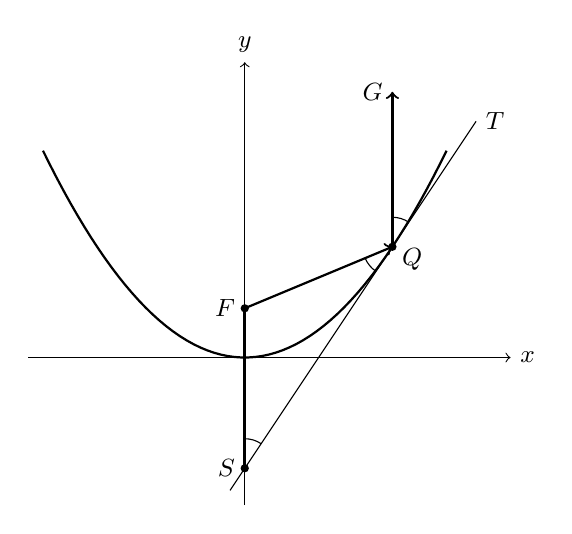
\begin{tikzpicture}[scale=1.25,font=\small]
\draw[->] (-2.2,0)--(2.7,0) node[right] {$x$};
\draw[->] (0,-1.5)--(0,3) node[above] {$y$};
\draw[thick,domain=-2.05:2.05,samples=60] plot (\x,{\x*\x/2});
\draw (-0.15,-1.35)--(2.35,2.4);
\draw[very thick] (0,-1.125)--(0,0.5);
\draw[->,thick] (0,0.5)--(1.5,1.125);
\draw[->,thick] (1.5,1.125)--(1.5,2.7);
\draw (0,-1.125) ++(56.31:0.3) arc (56.31:90:0.3);
\draw (1.5,1.125) ++(202.62:0.3) arc (202.62:236.31:0.3);
\draw (1.5,1.125) ++(56.31:0.3) arc (56.31:90:0.3);
\fill (0,0.5) circle (1.2pt);
\fill (1.5,1.125) circle (1.2pt);
\fill (0,-1.125) circle (1.2pt);
\node[left] at (0,0.5) {$F$};
\node[right] at (1.5,1.0) {$Q$};
\node[left] at (0,-1.125) {$S$};
\node[left] at (1.5,2.7) {$G$};
\node[right] at (2.35,2.4) {$T$};
\end{tikzpicture}
\end{center}

\begin{cnproof}
若 $x_0=0$, 光线沿对称轴射出, 反射后仍沿对称轴, 结论成立. 设 $x_0\ne0$, 则 $\displaystyle y_0=\frac{x_0^2}{2p}>0$. 在 $x_0$ 处的差商为
\[
\frac{(x_0+\Delta x)^2-x_0^2}{2p\,\Delta x}=\frac{2x_0+\Delta x}{2p}\to\frac{x_0}p\quad(\Delta x\to0),
\]
所以切线方程为
\[
y=y_0+\frac{x_0}p(x-x_0).
\]
设切线与 $y$ 轴交于 $S$, $T$ 是切线上的一点, 且 $Q$ 在 $S$ 与 $T$ 之间; $QG$ 是从 $Q$ 出发平行于 $y$ 轴向上的射线. 在切线方程中令 $x=0$, 由 $x_0^2=2py_0$ 得 $S$ 的纵坐标为 $\displaystyle y_0-\frac{x_0^2}p=-y_0$. 于是
\[
\begin{gathered}
FS=\frac p2-(-y_0)=y_0+\frac p2,\\
FQ=\sqrt{x_0^2+\left(y_0-\frac p2\right)^2}=\sqrt{2py_0+y_0^2-py_0+\frac{p^2}4}=\sqrt{\left(y_0+\frac p2\right)^2}=y_0+\frac p2.
\end{gathered}
\]
所以 $FS=FQ$, 从而 $\angle FQS=\angle FSQ$. 又 $QG$ 与 $SF$ 平行且同向, $\angle GQT=\angle FSQ$ (同位角), 所以 $\angle FQS=\angle GQT$, 即 $QG$ 与切线所成的角等于 $FQ$ 与切线所成的角. 由反射定律, 从 $F$ 射到 $Q$ 的光线沿 $QG$ 方向反射, 平行于对称轴.
\end{cnproof}
\begin{example}\label{ex:c2-h1-12}
\textnormal{(选自教材习题2.1第12题)} $a$ ($a>0$, $a\ne1$) 为何值时, 曲线 $y=a^x$ 与直线 $y=x$ 相切? 求出切点.
\end{example}
\begin{cnsolution}
曲线与直线在点 $(x_0,y_0)$ 相切, 是说这一点同在曲线和直线上, 并且曲线在这一点的切线斜率 $a^{x_0}\ln a$ 等于直线的斜率 $1$:
\[
a^{x_0}=x_0,\qquad a^{x_0}\ln a=1.
\]
把前一式代入后一式得 $x_0\ln a=1$, 于是 $a^{x_0}=e^{x_0\ln a}=e$, 再由前一式得 $x_0=e$, 从而 $\displaystyle\ln a=\frac1e$, $a=e^{\frac1e}$. 反过来, 当 $a=e^{\frac1e}$ 时 $a^e=e$, $a^e\ln a=1$, 两个条件都满足. 所以 $a=e^{\frac1e}$, 切点为 $(e,e)$.
\end{cnsolution}
两条曲线在交点处的\textbf{交角}, 是指它们在这一点的切线所成的角 (取不超过 $\displaystyle\frac\pi2$ 的那个); 交角为 $\displaystyle\frac\pi2$ 时称两条曲线在这一点\textbf{正交}. 两条切线的斜率 $k_1,k_2$ 都存在时, 正交就是 $k_1k_2=-1$.
\begin{example}\label{ex:c2-h1-11}
\textnormal{(选自教材习题2.1第11题)} 求双曲线 $\displaystyle y=\frac1x$ 与抛物线 $y=\sqrt x$ 的交角.
\end{example}
\begin{cnsolution}
由 $\displaystyle\frac1x=\sqrt x$ 得 $x^{\frac32}=1$, 交点为 $(1,1)$. 由例\ref{ex:c2-1-7}, 两条切线在交点处的斜率分别为
\[
k_1=-\frac1{x^2}\bigg|_{x=1}=-1,\qquad k_2=\frac1{2\sqrt x}\bigg|_{x=1}=\frac12.
\]
设两条切线的倾斜角分别为 $\alpha_1,\alpha_2$. 这里 $\displaystyle1+k_1k_2=\frac12\ne0$, 两条切线不垂直. 交角 $\theta$ 是 $|\alpha_2-\alpha_1|$ 与它的补角中较小的一个. 这两个角的正切只差一个符号, 而 $\tan\theta\ge0$, 因此 $\tan\theta=|\tan(\alpha_2-\alpha_1)|$. 由两角差的正切公式,
\[
\tan\theta=|\tan(\alpha_2-\alpha_1)|=\left|\frac{k_2-k_1}{1+k_1k_2}\right|=\left|\frac{\frac12+1}{1-\frac12}\right|=3,
\]
所以 $\theta=\arctan3$.
\end{cnsolution}
\subsection{变化率}
导数的定义不涉及变量的具体含义, 所以一个量对另一个量的变化率可以用导数表示. 下面是教材附录中其他学科的例子, 它们都是先求平均变化率, 再令自变量的增量趋于零.
\begin{example}\label{ex:c2-1-13}
\textnormal{(教材例1.13)} 设从时刻 $0$ 到时刻 $t$ 通过导线横截面的电量为 $q=q(t)$. 求时刻 $t_0$ 的电流强度.
\end{example}
\begin{cnsolution}
从 $t_0$ 到 $t_0+\Delta t$ 通过横截面的电量为 $\Delta q=q(t_0+\Delta t)-q(t_0)$, $\displaystyle\frac{\Delta q}{\Delta t}$ 是这段时间内的平均电流强度. 令 $\Delta t\to0$, 得时刻 $t_0$ 的电流强度 $\displaystyle i(t_0)=\lim_{\Delta t\to0}\frac{\Delta q}{\Delta t}=q'(t_0)$.
\end{cnsolution}
\begin{example}\label{ex:c2-1-14}
\textnormal{(教材例1.14)} 细杆位于 $x$ 轴的区间 $[0,l]$ 上, 杆上 $[0,x]$ 一段的质量为 $m=m(x)$. 求杆在点 $x_0$ 处的线密度.
\end{example}
\begin{cnsolution}
$\displaystyle\frac{\Delta m}{\Delta x}=\frac{m(x_0+\Delta x)-m(x_0)}{\Delta x}$ 是以 $x_0$ 与 $x_0+\Delta x$ 为端点的一段杆的平均线密度 (单位长度的质量), 点 $x_0$ 处的线密度为 $\displaystyle\rho(x_0)=\lim_{\Delta x\to0}\frac{\Delta m}{\Delta x}=m'(x_0)$. 杆均匀时 $m(x)=\rho x$, 差商 $\displaystyle\frac{\Delta m}{\Delta x}=\frac{\rho\Delta x}{\Delta x}=\rho$, 各点的线密度都等于常数 $\rho$.
\end{cnsolution}
\begin{example}\label{ex:c2-1-15}
\textnormal{(教材例1.15)} 在化学反应 $A+B\to C$ 中, 生成物 $C$ 的浓度 $[C]$ 是时间 $t$ 的函数. 求时刻 $t_0$ 的反应速度.
\end{example}
\begin{cnsolution}
$\Delta[C]$ 表示从 $t_0$ 到 $t_0+\Delta t$ 浓度的增量, $\displaystyle\frac{\Delta[C]}{\Delta t}$ 是这段时间内的平均反应速度, 时刻 $t_0$ 的反应速度为
\[
\lim_{\Delta t\to0}\frac{\Delta[C]}{\Delta t}=\left.\frac{\dd[C]}{\dd t}\right|_{t=t_0}.
\]
\end{cnsolution}
\begin{example}\label{ex:c2-1-16}
\textnormal{(教材例1.16)} 温度不变时, 一定量气体的体积 $V$ 是压强 $P$ 的函数 $V=V(P)$. 写出气体的等温压缩率.
\end{example}
\begin{cnsolution}
$\displaystyle\frac{\Delta V}{\Delta P}$ 是压强从 $P$ 变到 $P+\Delta P$ 时体积的平均变化率, 其极限 $\displaystyle\frac{\dd V}{\dd P}$ 是体积对压强的变化率. 压强增大时体积减小, 差商 $\displaystyle\frac{\Delta V}{\Delta P}<0$, 由极限的保序性, $\displaystyle\frac{\dd V}{\dd P}\le0$. 物理上用单位体积的变化率表示压缩的难易, 定义\textbf{等温压缩率}
\[
\beta=-\frac1V\cdot\frac{\dd V}{\dd P},
\]
负号使 $\beta$ 不取负值.
\end{cnsolution}
\begin{example}\label{ex:c2-1-17}
\textnormal{(教材例1.17)} 设某生物种群在时刻 $t$ 的数量为 $n=f(t)$. 求时刻 $t_0$ 的增长率.
\end{example}
\begin{cnsolution}
$\displaystyle\frac{f(t_0+\Delta t)-f(t_0)}{\Delta t}$ 是从 $t_0$ 到 $t_0+\Delta t$ 这段时间内的平均增长率, 时刻 $t_0$ 的增长率为 $f'(t_0)$. 种群数量只取整数值, $f$ 在数量发生变化的时刻不连续, 因而在这些时刻不可导. 只有把 $f$ 近似看作可导函数, 才能用导数表示增长率; 数量很大时可以这样近似.
\end{cnsolution}
\begin{example}\label{ex:c2-1-18}
\textnormal{(教材例1.18)} 血液在半径为 $R$、长为 $l$ 的血管中流动, 两端的压强差为 $P$, 血液的黏度为 $\eta$. 由层流定律, 离血管轴线距离为 $r$ ($0\le r\le R$) 处的流速为
\[
v=\frac P{4\eta l}\left(R^2-r^2\right).
\]
求流速对 $r$ 的变化率 (速度梯度). 对 $\eta=0.027$, $R=0.008$ cm, $l=2$ cm, $P=4000$ (厘米-克-秒单位制), 求 $r=0.002$ cm 处的流速和速度梯度.
\end{example}
\begin{cnsolution}
由定义,
\[
\frac{\Delta v}{\Delta r}=\frac P{4\eta l}\cdot\frac{\left(R^2-(r+\Delta r)^2\right)-\left(R^2-r^2\right)}{\Delta r}=-\frac P{4\eta l}(2r+\Delta r)\to-\frac{Pr}{2\eta l}\quad(\Delta r\to0),
\]
即 $\displaystyle\frac{\dd v}{\dd r}=-\frac{Pr}{2\eta l}$. 负号与离轴线越远流速越小相符 (由 $v$ 的表达式, $r$ 越大, $R^2-r^2$ 越小). 代入数据, $\displaystyle\frac P{4\eta l}=\frac{4000}{0.216}\approx1.85\times10^4$, 在 $r=0.002$ 处
\[
\begin{gathered}
v\approx1.85\times10^4\times\left(6.4\times10^{-5}-4\times10^{-6}\right)\approx1.11\ \text{cm/s},\\
\frac{\dd v}{\dd r}=-\frac{4000\times0.002}{2\times0.027\times2}\approx-74\ \text{(cm/s)/cm}.
\end{gathered}
\]
\end{cnsolution}
\begin{example}\label{ex:c2-1-19}
\textnormal{(教材例1.19)} 设生产 $x$ 件产品的总成本为 $C=C(x)$. 写出边际成本的定义.
\end{example}
\begin{cnsolution}
产量从 $x$ 增加到 $x+\Delta x$ 时, 成本的增量为 $\Delta C=C(x+\Delta x)-C(x)$, $\displaystyle\frac{\Delta C}{\Delta x}$ 是这部分产品每件的平均成本. 经济学中把产量为 $x$ 时成本对产量的变化率 $C'(x)$ 称为\textbf{边际成本}. 产量很大时, 一件产品可以看作很小的增量, 所以 $\Delta x=1$ 时的差商 $C(x+1)-C(x)$ 近似等于 $C'(x)$, 即边际成本近似等于在产量 $x$ 的基础上再多生产一件产品所增加的成本.
\end{cnsolution}
\section{求导法则与导数基本公式}
用定义求导数, 每次都要计算一个 $\displaystyle\frac00$ 型的极限. 本节建立四则运算、反函数和复合函数的求导法则, 由它们和 2.1 节的几个公式可以求出全部基本初等函数的导数. 初等函数由基本初等函数经有限次四则运算和复合得到, 所以初等函数的导数一般也可以由这些法则求出, 不必每次回到定义.
\subsection{导数的四则运算法则}
\begin{theorem}[四则运算法则]\label{thm:c2-2-arith}
设 $u=u(x)$, $v=v(x)$ 都在点 $x$ 可导. 则 $u\pm v$ 与 $uv$ 在 $x$ 可导; 若还有 $v(x)\ne0$, 则 $\displaystyle\frac uv$ 也在 $x$ 可导. 并且
\[
\text{(1)}\ (u\pm v)'=u'\pm v';\qquad\text{(2)}\ (uv)'=u'v+uv';\qquad\text{(3)}\ \left(\frac uv\right)'=\frac{u'v-uv'}{v^2}.
\]
\end{theorem}
\par\indent\textbf{分析:} 已知的是 $\displaystyle\frac{\Delta u}{\Delta x}\to u'$, $\displaystyle\frac{\Delta v}{\Delta x}\to v'$, 其中 $\Delta u=u(x+\Delta x)-u(x)$, $\Delta v=v(x+\Delta x)-v(x)$. 所以要把和、差、积、商的增量用 $\Delta u$, $\Delta v$ 表示. (1) 中, 和的增量就是增量之和. (2) 中, 乘积从 $u(x)v(x)$ 变到 $u(x+\Delta x)v(x+\Delta x)$, 两个因子同时改变, 可以让它们先后改变. 先只改变 $v$, 乘积变到 $u(x)v(x+\Delta x)$, 增量是 $u(x)\cdot\Delta v$; 再只改变 $u$, 乘积变到 $u(x+\Delta x)v(x+\Delta x)$, 增量是 $\Delta u\cdot v(x+\Delta x)$. 两次的增量相加就是乘积的增量, 也就是减去再加上中间项 $u(x)v(x+\Delta x)$:
\[
u(x+\Delta x)v(x+\Delta x)-u(x)v(x)=\Delta u\cdot v(x+\Delta x)+u(x)\cdot\Delta v,
\]
除以 $\Delta x$ 后, $v(x+\Delta x)$ 的极限由 $v$ 在 $x$ 连续 (2.1 节可导必连续的定理) 得到. (3) 中, 商的增量通分后, 分子为 $u(x+\Delta x)v(x)-u(x)v(x+\Delta x)$, 两项的对应因子都不相同. 同样减去再加上只改变一个因子的中间项 $u(x)v(x)$, 分子化为 $\Delta u\cdot v(x)-u(x)\cdot\Delta v$. 分母是 $v(x+\Delta x)v(x)$, 还要保证 $|\Delta x|$ 很小时 $v(x+\Delta x)\ne0$, 这由 $v$ 在 $x$ 连续及保号性得到.
\begin{cnproof}
(1) 由极限的和、差法则, $\displaystyle(u\pm v)'=\lim_{\Delta x\to0}\left(\frac{\Delta u}{\Delta x}\pm\frac{\Delta v}{\Delta x}\right)=u'\pm v'$.

(2) 由 $v$ 在 $x$ 可导知 $v$ 在 $x$ 连续, $\displaystyle\lim_{\Delta x\to0}v(x+\Delta x)=v(x)$. 于是
\[
(uv)'=\lim_{\Delta x\to0}\left[\frac{\Delta u}{\Delta x}\cdot v(x+\Delta x)+u(x)\cdot\frac{\Delta v}{\Delta x}\right]=u'v+uv'.
\]

(3) $v$ 在 $x$ 连续且 $v(x)\ne0$, 由保号性, $|\Delta x|$ 充分小时 $v(x+\Delta x)\ne0$. 这时
\[
\frac{u(x+\Delta x)}{v(x+\Delta x)}-\frac{u(x)}{v(x)}=\frac{u(x+\Delta x)v(x)-u(x)v(x+\Delta x)}{v(x+\Delta x)v(x)}=\frac{\Delta u\cdot v(x)-u(x)\cdot\Delta v}{v(x+\Delta x)v(x)},
\]
第二个等号是在分子中减去再加上 $u(x)v(x)$. 除以 $\Delta x$, 令 $\Delta x\to0$, 得
\[
\left(\frac uv\right)'=\lim_{\Delta x\to0}\frac1{v(x+\Delta x)v(x)}\left[\frac{\Delta u}{\Delta x}v(x)-u(x)\frac{\Delta v}{\Delta x}\right]=\frac{u'v-uv'}{v^2}.
\]
\end{cnproof}
乘积的求导法则可以用矩形的面积来理解. 设 $u,v>0$, 把 $uv$ 看作边长为 $u$, $v$ 的矩形的面积. 两边分别增加 $\Delta u$, $\Delta v$ 时, 面积的增量由两个长条 $\Delta u\cdot v$, $u\cdot\Delta v$ 和角上的小矩形 $\Delta u\Delta v$ 组成. 两个长条除以 $\Delta x$ 后分别趋于 $u'v$ 与 $uv'$; 小矩形除以 $\Delta x$ 后, $\displaystyle\frac{\Delta u\Delta v}{\Delta x}=\frac{\Delta u}{\Delta x}\cdot\Delta v\to u'\cdot0=0$. 所以乘积的导数中只有两项, 没有 $u'v'$ 这一项.

在 (2) 中取 $v=C$ 为常数, 由 $(C)'=0$ 得 $(Cu)'=Cu'$; 在 (3) 中取 $u=1$, 得 $\displaystyle\left(\frac1v\right)'=-\frac{v'}{v^2}$. 法则 (1)(2) 还可以推广到有限个函数, 例如
\[
(u+v+w)'=u'+v'+w',\qquad(uvw)'=(uv)'w+uvw'=u'vw+uv'w+uvw'.
\]
\begin{example}\label{ex:c2-2-1}
\textnormal{(教材例2.1)} 求 $\displaystyle y=\frac2{\sqrt x}-3\sin x+7$ 的导数.
\end{example}
\begin{cnsolution}
由和、差与常数倍的法则, $\displaystyle y'=2\left(x^{-\frac12}\right)'-3(\sin x)'+(7)'=-x^{-\frac32}-3\cos x=-\frac1{x\sqrt x}-3\cos x$.
\end{cnsolution}
\begin{example}\label{ex:c2-2-2}
\textnormal{(教材例2.2)} 求 $y=3\cos x\ln x$ 的导数.
\end{example}
\begin{cnsolution}
由常数倍与乘积的法则, $\displaystyle y'=3\left[(\cos x)'\ln x+\cos x(\ln x)'\right]=3\left(-\sin x\ln x+\frac{\cos x}x\right)$.
\end{cnsolution}
\begin{example}\label{ex:c2-2-3}
\textnormal{(教材例2.3)} 求 $\tan x$ 与 $\cot x$ 的导数.
\end{example}
\begin{cnsolution}
正切是正弦与余弦之商, 用商的法则. 在 $\cos x\ne0$ 处,
\[
(\tan x)'=\left(\frac{\sin x}{\cos x}\right)'=\frac{\cos x\cdot\cos x-\sin x\cdot(-\sin x)}{\cos^2x}=\frac1{\cos^2x}=\sec^2x.
\]
同理, 在 $\sin x\ne0$ 处 $\displaystyle(\cot x)'=\frac{-\sin x\cdot\sin x-\cos x\cdot\cos x}{\sin^2x}=-\frac1{\sin^2x}=-\csc^2x$.
\end{cnsolution}
\begin{example}\label{ex:c2-2-4}
\textnormal{(教材例2.4)} 求 $\sec x$ 与 $\csc x$ 的导数.
\end{example}
\begin{cnsolution}
由倒数的求导公式, 在 $\cos x\ne0$ 处 $\displaystyle(\sec x)'=\left(\frac1{\cos x}\right)'=\frac{\sin x}{\cos^2x}=\sec x\tan x$; 在 $\sin x\ne0$ 处 $\displaystyle(\csc x)'=\left(\frac1{\sin x}\right)'=-\frac{\cos x}{\sin^2x}=-\csc x\cot x$.
\end{cnsolution}
\subsection{反函数的求导法则}
函数 $y=f(x)$ 与它的反函数 $x=\varphi(y)$ 的图像是同一条曲线, 只是自变量换成了 $y$. 设曲线在点 $(x_0,y_0)$ 处的切线不平行于坐标轴. 沿切线, 纵坐标的改变量与横坐标的改变量之比是 $f'(x_0)$, 横坐标的改变量与纵坐标的改变量之比是 $\varphi'(y_0)$, 两者互为倒数. 下图画的是 $f(x)=x^2$ ($x>0$) 与 $\varphi(y)=\sqrt y$ 在点 $M(1,1)$ 处的情形. 切线 $y=2x-1$ 与 $x$ 轴正向、$y$ 轴正向的夹角 $\alpha$, $\beta$ 互余, 所以 $\tan\alpha=f'(1)=2$ 与 $\displaystyle\tan\beta=\varphi'(1)=\frac12$ 互为倒数.
\begin{center}
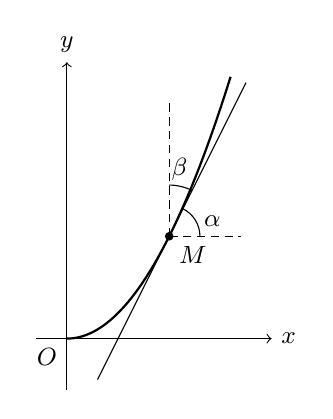
\begin{tikzpicture}[scale=1.3,font=\small]
\draw[->] (-0.3,0)--(2,0) node[right] {$x$};
\draw[->] (0,-0.5)--(0,2.7) node[above] {$y$};
\draw[thick,domain=0:1.6,samples=50] plot (\x,{\x*\x});
\draw (0.3,-0.4)--(1.75,2.5);
\draw[densely dashed] (1,1)--(1.7,1);
\draw[densely dashed] (1,1)--(1,2.3);
\fill (1,1) circle (1.2pt);
\draw (1.3,1) arc[start angle=0,end angle=63.43,radius=0.3];
\draw (1,1.5) arc[start angle=90,end angle=63.43,radius=0.5];
\node at (1.42,1.15) {$\alpha$};
\node at (1.1,1.65) {$\beta$};
\node[below right] at (1,1) {$M$};
\node[below left] at (0,0) {$O$};
\end{tikzpicture}
\end{center}

若切线平行于 $y$ 轴, 则 $\varphi'(y_0)=0$, 而 $f$ 在 $x_0$ 的导数为无穷大, 例如 $x=y^3$ 与 $y=\sqrt[3]x$ 在原点处 (2.1 节). 下面的定理要求 $\varphi'(y_0)\ne0$, 就是为了排除这种情形.
\begin{theorem}[反函数的求导法则]\label{thm:c2-2-inv}
设 $x=\varphi(y)$ 在 $y_0$ 的某个邻域内连续且严格单调, 在 $y_0$ 处可导且 $\varphi'(y_0)\ne0$. 则 $\varphi$ 在这个邻域上的反函数 $y=f(x)$ 在对应点 $x_0=\varphi(y_0)$ 处可导, 并且
\[
f'(x_0)=\frac1{\varphi'(y_0)},\qquad\text{即}\quad\frac{\dd y}{\dd x}=\frac1{\displaystyle\frac{\dd x}{\dd y}}.
\]
\end{theorem}
\par\indent\textbf{分析:} 要求的是 $\displaystyle\frac{\Delta y}{\Delta x}$ 在 $\Delta x\to0$ 时的极限, 其中 $\Delta y=f(x_0+\Delta x)-f(x_0)$. 已知的是 $\displaystyle\frac{\varphi(y_0+\Delta y)-\varphi(y_0)}{\Delta y}\to\varphi'(y_0)$ ($\Delta y\to0$). 由 $y_0+\Delta y=f(x_0+\Delta x)$ 得 $x_0+\Delta x=\varphi(y_0+\Delta y)$, 再减去 $x_0=\varphi(y_0)$, 就有 $\Delta x=\varphi(y_0+\Delta y)-\varphi(y_0)$, 所以这两个比值互为倒数:
\[
\frac{\Delta y}{\Delta x}=\frac1{\displaystyle\frac{\varphi(y_0+\Delta y)-\varphi(y_0)}{\Delta y}}.
\]
由 $\varphi'(y_0)\ne0$, 右端在 $\Delta y\to0$ 时趋于 $\displaystyle\frac1{\varphi'(y_0)}$. 但要求的极限中变量是 $\Delta x$, 已知的极限中变量是 $\Delta y$. 按 1.6 节复合函数的极限, 要检查两点: $\Delta x\to0$ 时 $\Delta y\to0$, 即反函数 $f$ 在 $x_0$ 连续, 这由 1.8 节反函数的连续性得到; $\Delta x\ne0$ 时 $\Delta y\ne0$, 这由严格单调得到. 此外, 按导数的定义, 还要说明 $f$ 在 $x_0$ 的某个邻域内有定义, 这要用到 $\varphi$ 在邻域内连续以及 1.9 节的介值定理.
\begin{cnproof}
设 $\varphi$ 在 $U(y_0,r)$ 内连续且严格增加 (严格减少的情形把不等号反向). 在这个邻域内取闭区间 $\displaystyle\left[y_0-\frac r2,y_0+\frac r2\right]$, 记
\[
p=\varphi\left(y_0-\frac r2\right),\qquad q=\varphi\left(y_0+\frac r2\right),
\]
则 $p<x_0<q$. 由 1.9 节的介值定理, $(p,q)$ 中的每个数都是 $\varphi$ 在这个闭区间上的函数值, 所以反函数 $f$ 在含 $x_0$ 的开区间 $(p,q)$ 内有定义. 取 $\rho=\min\{x_0-p,q-x_0\}$, 则 $U(x_0,\rho)\subseteq(p,q)$, $f$ 在 $x_0$ 的这个邻域内有定义. 由 1.8 节反函数的连续性, $f$ 在 $(p,q)$ 内严格增加且连续.

当 $x_0+\Delta x\in(p,q)$, $\Delta x\ne0$ 时, 由 $f$ 严格增加, $\Delta y=f(x_0+\Delta x)-f(x_0)\ne0$, 并且 $\Delta x=\varphi(y_0+\Delta y)-\varphi(y_0)$. 由 $f$ 在 $x_0$ 连续, $\Delta x\to0$ 时 $\Delta y\to0$. 由复合函数的极限及 $\varphi'(y_0)\ne0$,
\[
f'(x_0)=\lim_{\Delta x\to0}\frac{\Delta y}{\Delta x}=\frac1{\displaystyle\lim_{\Delta y\to0}\frac{\varphi(y_0+\Delta y)-\varphi(y_0)}{\Delta y}}=\frac1{\varphi'(y_0)}.
\]
\end{cnproof}
\begin{example}\label{ex:c2-2-5}
\textnormal{(教材例2.5)} 求 $\arcsin x$ 与 $\arccos x$ 的导数.
\end{example}
\begin{cnsolution}
$y=\arcsin x$ ($-1<x<1$) 是 $x=\sin y$ 在 $\displaystyle\left(-\frac\pi2,\frac\pi2\right)$ 上的反函数. 在这个区间内 $\sin y$ 连续、严格增加, $(\sin y)'=\cos y>0$, 满足定理\ref{thm:c2-2-inv} 的条件. 由 $\cos y>0$ 得 $\cos y=\sqrt{1-\sin^2y}=\sqrt{1-x^2}$, 所以
\[
(\arcsin x)'=\frac1{(\sin y)'}=\frac1{\cos y}=\frac1{\sqrt{1-x^2}}\quad(-1<x<1).
\]
同样, $y=\arccos x$ 是 $x=\cos y$ 在 $(0,\pi)$ 上的反函数, $(\cos y)'=-\sin y<0$, $\sin y=\sqrt{1-x^2}$, 所以 $\displaystyle(\arccos x)'=-\frac1{\sqrt{1-x^2}}$ ($-1<x<1$). 在 $x=\pm1$ 处, 对应的 $\cos y$ (或 $\sin y$) 为零, 不满足定理的条件 $\varphi'(y_0)\ne0$; 几何上, 曲线在这两点的切线平行于 $y$ 轴.
\end{cnsolution}
\begin{example}\label{ex:c2-2-6}
\textnormal{(教材例2.6)} 求 $\arctan x$ 与 $\operatorname{arccot}x$ 的导数.
\end{example}
\begin{cnsolution}
$y=\arctan x$ 是 $x=\tan y$ 在 $\displaystyle\left(-\frac\pi2,\frac\pi2\right)$ 上的反函数, $\tan y$ 在这个区间内连续、严格增加, $(\tan y)'=\sec^2y>0$, 所以
\[
(\arctan x)'=\frac1{\sec^2y}=\frac1{1+\tan^2y}=\frac1{1+x^2}.
\]
$y=\operatorname{arccot}x$ 是 $x=\cot y$ 在 $(0,\pi)$ 上的反函数, $(\cot y)'=-\csc^2y<0$, 所以 $\displaystyle(\operatorname{arccot}x)'=-\frac1{\csc^2y}=-\frac1{1+\cot^2y}=-\frac1{1+x^2}$.
\end{cnsolution}
\begin{example}\label{ex:c2-h2-7}
\textnormal{(指定作业: 习题2.2第7题)} 设 $x=\varphi(y)$ 与 $y=f(x)$ 互为反函数, $f$ 在 $1$ 的某个邻域内连续且严格单调, $\varphi(2)=1$, $f'(1)=3$. 求 $\varphi'(2)$.
\end{example}
\begin{cnsolution}
教材原题没有给出 $f$ 在 $1$ 附近连续且严格单调, 这里补上这个条件, 才能用定理\ref{thm:c2-2-inv}. 由 $\varphi(2)=1$ 知 $f(1)=2$, 即 $x=1$ 与 $y=2$ 是对应点. 又 $f'(1)=3\ne0$, 把定理\ref{thm:c2-2-inv} 用于 $f$ 和它的反函数 $\varphi$, 得 $\displaystyle\varphi'(2)=\frac1{f'(1)}=\frac13$. 两个导数要在对应点处取值, 不能写成 $\displaystyle\frac1{f'(2)}$.
\end{cnsolution}
至此得到了全部基本初等函数的导数:
\[
\begin{aligned}
&(C)'=0, &&(x^\mu)'=\mu x^{\mu-1},\\
&(a^x)'=a^x\ln a, &&(e^x)'=e^x,\\
&(\log_ax)'=\frac1{x\ln a}, &&(\ln x)'=\frac1x,\\
&(\sin x)'=\cos x, &&(\cos x)'=-\sin x,\\
&(\tan x)'=\sec^2x, &&(\cot x)'=-\csc^2x,\\
&(\sec x)'=\sec x\tan x, &&(\csc x)'=-\csc x\cot x,\\
&(\arcsin x)'=\frac1{\sqrt{1-x^2}}, &&(\arccos x)'=-\frac1{\sqrt{1-x^2}},\\
&(\arctan x)'=\frac1{1+x^2},\qquad &&(\operatorname{arccot}x)'=-\frac1{1+x^2}.
\end{aligned}
\]
\subsection{复合函数的求导法则}
$\sin2x$, $\sqrt[3]{1-2x^2}$ 这类函数由基本初等函数经复合得到. 前者可以先化成 $2\sin x\cos x$, 由乘积的法则得 $(\sin2x)'=2(\cos^2x-\sin^2x)=2\cos2x$; 后者不便化成乘积, 要另找办法. 若把 $2x$ 看作整体, 只对正弦求导, 得到的是 $\cos2x$, 少了因子 $2$. $x$ 改变 $\Delta x$ 时, $u=2x$ 改变 $2\Delta x$, 所以 $\sin u$ 对 $x$ 的变化率是它对 $u$ 的变化率 $\cos u$ 的 $2$ 倍, 这个 $2$ 正是里层函数 $2x$ 的导数. 下面的定理对一般的复合函数给出求导法则.
\begin{theorem}[复合函数的求导法则]\label{thm:c2-2-chain}
设 $u=\varphi(x)$ 在点 $x$ 可导, $y=f(u)$ 在对应点 $u=\varphi(x)$ 可导. 则复合函数 $y=f(\varphi(x))$ 在点 $x$ 可导, 并且
\[
\bigl[f(\varphi(x))\bigr]'=f'(\varphi(x))\,\varphi'(x),\qquad\text{即}\quad\frac{\dd y}{\dd x}=\frac{\dd y}{\dd u}\cdot\frac{\dd u}{\dd x}.
\]
\end{theorem}
\par\indent\textbf{分析:} 记 $\Delta u=\varphi(x+\Delta x)-\varphi(x)$, $\Delta y=f(u+\Delta u)-f(u)$. 当 $\Delta u\ne0$ 时可以写
\[
\frac{\Delta y}{\Delta x}=\frac{\Delta y}{\Delta u}\cdot\frac{\Delta u}{\Delta x},
\]
第二个因子趋于 $\varphi'(x)$. 第一个因子是 $f$ 在 $u$ 处的差商, 可以看作增量 $k$ 的函数 $\displaystyle\frac{f(u+k)-f(u)}k$ 在 $k=\Delta u$ 处的值. 由 $\varphi$ 在 $x$ 连续, $\Delta x\to0$ 时 $\Delta u\to0$; 按 1.6 节复合函数的极限, 若还有 $\Delta x\ne0$ 时 $\Delta u\ne0$, 第一个因子就趋于 $f'(u)$. 但这个条件可能不成立. 例如设 $\displaystyle\varphi(x)=x^2\sin\frac1x$ ($x\ne0$), $\varphi(0)=0$. 它在 $0$ 处的差商 $\displaystyle\Delta x\sin\frac1{\Delta x}\to0$, 所以在 $0$ 可导; 但在 $x=0$ 处取 $\displaystyle\Delta x=\frac1{n\pi}$ 时 $\Delta u=0$. 这样的 $\Delta x$ 可以任意小, 所以无论把 $|\Delta x|$ 限制得多小, 都会出现 $\Delta u=0$, 这时 $\displaystyle\frac{\Delta y}{\Delta u}$ 没有意义.

由 1.6 节复合函数极限定理后面的说明, 若差商作为 $k$ 的函数在 $k=0$ 连续, 就不需要 $\Delta u\ne0$ 这个条件. 差商在 $k=0$ 处没有定义, 但在 $k\to0$ 时趋于 $f'(u)$, 所以在 $k=0$ 处补充定义它的值为 $f'(u)$, 就得到在 $k=0$ 连续的函数
\[
\psi(k)=\begin{cases}\frac{f(u+k)-f(u)}k,&k\ne0,\\f'(u),&k=0.\end{cases}
\]
等式 $\Delta y=\psi(\Delta u)\,\Delta u$ 在 $\Delta u\ne0$ 时由 $\psi$ 的定义成立, 在 $\Delta u=0$ 时两边都是 $0$, 也成立. 于是
\[
\frac{\Delta y}{\Delta x}=\psi(\Delta u)\cdot\frac{\Delta u}{\Delta x}
\]
不再要求 $\Delta u\ne0$, 并且 $\Delta x\to0$ 时 $\psi(\Delta u)\to\psi(0)=f'(u)$.
\begin{cnproof}
设 $f$ 在 $U(u,r)$ 内有定义. 由 2.1 节可导必连续的定理, $\varphi$ 在 $x$ 连续, 所以 $|\Delta x|$ 充分小时 $|\Delta u|<r$, 复合函数在 $x+\Delta x$ 处有定义. 令 $\displaystyle\psi(k)=\frac{f(u+k)-f(u)}k$ ($0<|k|<r$), $\psi(0)=f'(u)$. 由导数的定义, $\displaystyle\lim_{k\to0}\psi(k)=f'(u)=\psi(0)$, 即 $\psi$ 在 $0$ 连续. 当 $0<|k|<r$ 时 $f(u+k)-f(u)=\psi(k)\,k$; $k=0$ 时这个等式两边都是 $0$, 也成立. 取 $k=\Delta u$, 两边除以 $\Delta x$, 得
\[
\frac{\Delta y}{\Delta x}=\psi(\Delta u)\cdot\frac{\Delta u}{\Delta x}.
\]
当 $\Delta x\to0$ 时 $\Delta u\to0$. 由于 $\psi$ 在 $0$ 连续, 按 1.6 节复合函数极限定理后面的说明, 即使 $\Delta u$ 可能等于零, 也有 $\displaystyle\lim_{\Delta x\to0}\psi(\Delta u)=\psi(0)=f'(u)$. 又 $\displaystyle\lim_{\Delta x\to0}\frac{\Delta u}{\Delta x}=\varphi'(x)$, 由极限的积的法则,
\[
\bigl[f(\varphi(x))\bigr]'=\lim_{\Delta x\to0}\frac{\Delta y}{\Delta x}=\lim_{\Delta x\to0}\psi(\Delta u)\cdot\lim_{\Delta x\to0}\frac{\Delta u}{\Delta x}=f'(u)\varphi'(x).
\]
\end{cnproof}
多次复合时逐层应用定理. 例如 $y=f(u)$, $u=g(v)$, $v=h(x)$ 都可导时,
\[
\frac{\dd y}{\dd x}=\frac{\dd y}{\dd u}\cdot\frac{\dd u}{\dd v}\cdot\frac{\dd v}{\dd x},
\]
各个导数在对应点处取值. 复合函数的求导法则也称为\textbf{链式法则}.
\begin{example}\label{ex:c2-2-7}
\textnormal{(教材例2.7)} 求 $y=\sin2x$ 的导数.
\end{example}
\begin{cnsolution}
$y=\sin u$, $u=2x$, 所以 $\displaystyle y'=\frac{\dd y}{\dd u}\cdot\frac{\dd u}{\dd x}=\cos u\cdot2=2\cos2x$.
\end{cnsolution}
\begin{example}\label{ex:c2-2-8}
\textnormal{(教材例2.8)} 求 $y=\sqrt[3]{1-2x^2}$ 的导数.
\end{example}
\begin{cnsolution}
$y=u^{\frac13}$, $u=1-2x^2$. 在 $u\ne0$, 即 $\displaystyle x\ne\pm\frac1{\sqrt2}$ 处,
\[
y'=\frac13u^{-\frac23}\cdot(-4x)=-\frac{4x}{3\sqrt[3]{(1-2x^2)^2}}.
\]
\end{cnsolution}
\begin{example}\label{ex:c2-2-9}
\textnormal{(教材例2.9)} 求 $y=\tan\bigl[\ln(1+x^2)\bigr]$ 的导数.
\end{example}
\begin{cnsolution}
函数由 $y=\tan u$, $u=\ln v$, $v=1+x^2$ 三层复合而成. 由链式法则,
\[
y'=\sec^2u\cdot\frac1v\cdot2x=\frac{2x}{(1+x^2)\cos^2\bigl[\ln(1+x^2)\bigr]}.
\]
\end{cnsolution}
熟练以后不必写出中间变量. 从最外层开始, 把里面的部分看作一个整体, 对这一层求导, 再乘以里面部分的导数; 里面部分的导数按同样的办法求, 一层一层直到最里层的 $x$, 每一层都不能遗漏.
\begin{example}\label{ex:c2-2-10}
\textnormal{(教材例2.10)} 求 $y=\ln|x|$ ($x\ne0$) 的导数.
\end{example}
\begin{cnsolution}
当 $x>0$ 时, $\displaystyle(\ln|x|)'=(\ln x)'=\frac1x$; 当 $x<0$ 时, $\ln|x|=\ln(-x)$, 由链式法则 $\displaystyle(\ln(-x))'=\frac1{-x}\cdot(-1)=\frac1x$. 所以 $\displaystyle(\ln|x|)'=\frac1x$ ($x\ne0$).
\end{cnsolution}
\begin{example}\label{ex:c2-2-11}
\textnormal{(教材例2.11)} 设 $\displaystyle f(t)=\lim_{x\to\infty}t\left(1+\frac1x\right)^{2t^2x}$, 求 $f'(t)$.
\end{example}
\begin{cnsolution}
函数由极限给出, 先求极限. 对固定的 $t\ne0$, 这是 $1^\infty$ 型. 把幂写成 $\displaystyle\left(1+\frac1x\right)^x$ 的 $2t^2$ 次幂:
\[
\left(1+\frac1x\right)^{2t^2x}=\left[\left(1+\frac1x\right)^x\right]^{2t^2},
\]
这个等式在 $t=0$ 时也成立. 由第二个重要极限, 方括号内趋于 $e$; 方括号外的指数 $2t^2$ 与 $x$ 无关, 由 1.6 节幂指函数的极限, 整个式子趋于 $e^{2t^2}$. 所以对一切 $t$ 有 $f(t)=te^{2t^2}$. 于是
\[
f'(t)=e^{2t^2}+t\cdot e^{2t^2}\cdot4t=(1+4t^2)e^{2t^2}.
\]
\end{cnsolution}
\begin{example}\label{ex:c2-2-12}
\textnormal{(教材例2.12)} 求 $y=3^{\sin^2\frac1x}$ 的导数.
\end{example}
\begin{cnsolution}
函数由外向内依次是指数函数、平方、正弦和 $\displaystyle\frac1x$, 逐层求导, 得
\[
y'=3^{\sin^2\frac1x}\ln3\cdot2\sin\frac1x\cdot\cos\frac1x\cdot\left(-\frac1{x^2}\right)=-\frac{\ln3}{x^2}\sin\frac2x\cdot3^{\sin^2\frac1x}.
\]
\end{cnsolution}
\begin{example}\label{ex:c2-2-13}
\textnormal{(教材例2.13)} 求 $y=\ln\left(x+\sqrt{1+x^2}\right)$ 的导数.
\end{example}
\begin{cnsolution}
外层是对数, 真数 $x+\sqrt{1+x^2}$ 对一切 $x$ 为正 (因为 $\sqrt{1+x^2}>|x|$). 由链式法则, 先对对数求导, 再乘以真数的导数, 其中 $\displaystyle\left(\sqrt{1+x^2}\right)'=\frac{2x}{2\sqrt{1+x^2}}$. 于是
\[
y'=\frac1{x+\sqrt{1+x^2}}\left(1+\frac{2x}{2\sqrt{1+x^2}}\right)=\frac1{x+\sqrt{1+x^2}}\cdot\frac{\sqrt{1+x^2}+x}{\sqrt{1+x^2}}=\frac1{\sqrt{1+x^2}}.
\]
\end{cnsolution}
\begin{example}\label{ex:c2-h2-3}
\textnormal{(指定作业: 习题2.2第3题)} 求下列函数的导数:
\[
\begin{aligned}
&\text{(1)}\ y=a^{b^x}+x^{a^b}+b^{x^a}\quad(x,a,b>0,\ a,b\text{ 为常数});\\
&\text{(2)}\ y=\lim_{n\to\infty}x\left(\frac{n+x}{n-x}\right)^n;\qquad\text{(3)}\ y=\begin{cases}1-x,&x\le0,\\e^{-x}\cos3x,&x>0.\end{cases}
\end{aligned}
\]
\end{example}
\begin{cnsolution}
(1) 先分清每一项中 $x$ 的位置. $a^{b^x}$ 的底数是常数, 指数 $b^x$ 是指数函数; $x^{a^b}$ 的指数 $a^b$ 是常数, 所以 $x^{a^b}$ 是幂函数, 不是指数函数; $b^{x^a}$ 的底数是常数, 指数 $x^a$ 是幂函数. 由指数函数、幂函数的导数公式和链式法则,
\[
y'=a^{b^x}\ln a\cdot b^x\ln b+a^bx^{a^b-1}+b^{x^a}\ln b\cdot ax^{a-1}.
\]

(2) 先对每个固定的 $x$ 算出这个数列的极限. $x=0$ 时 $y=0$. 设 $x\ne0$. 当 $n>|x|$ 时 $n+x>0$, $n-x>0$, 底数 $\displaystyle\frac{n+x}{n-x}$ 为正并且趋于 $1$, 指数 $n$ 无限增大, 是 $1^\infty$ 型. 按 1.6 节的办法, 令 $t_n$ 等于底数减 $1$:
\[
t_n=\frac{n+x}{n-x}-1=\frac{2x}{n-x},
\]
则 $t_n\ne0$, $t_n\to0$, 并且 $\displaystyle nt_n=\frac{2xn}{n-x}\to2x$. 由海涅定理, $(1+t_n)^{\frac1{t_n}}\to e$, 再由数列情形的幂指函数的极限,
\[
\left(\frac{n+x}{n-x}\right)^n=\Bigl[(1+t_n)^{\frac1{t_n}}\Bigr]^{nt_n}\to e^{2x}.
\]
因此 $y=xe^{2x}$ 对一切 $x$ 成立, 求导得 $y'=e^{2x}+2xe^{2x}=(1+2x)e^{2x}$.

(3) 在 $x<0$ 与 $x>0$ 处分别用相应的表达式求导:
\[
y'=-1\ \ (x<0),\qquad y'=-e^{-x}\cos3x-3e^{-x}\sin3x=-e^{-x}(\cos3x+3\sin3x)\ \ (x>0).
\]
分段点 $0$ 处要按定义求单侧导数. $y(0)=1$. 当 $h<0$ 时 $\displaystyle\frac{y(h)-y(0)}h=\frac{(1-h)-1}h=-1$, 所以 $y'_-(0)=-1$. 右侧的表达式 $g(x)=e^{-x}\cos3x$ 在 $0$ 处的值是 $1$, 等于 $y(0)$, 所以当 $h>0$ 时
\[
\frac{y(h)-y(0)}h=\frac{g(h)-g(0)}h\to g'(0)=-1,
\]
即 $y'_+(0)=-1$. 左、右导数相等, $y'(0)=-1$. 所以
\[
y'=\begin{cases}-1,&x\le0,\\-e^{-x}(\cos3x+3\sin3x),&x>0.\end{cases}
\]
\end{cnsolution}
\begin{example}\label{ex:c2-2-14}
\textnormal{(教材例2.14)} 已知 $\displaystyle y=f\left(\frac{3x-2}{3x+2}\right)$, $f'(x)=\arctan x^2$, 求 $\displaystyle\left.\frac{\dd y}{\dd x}\right|_{x=0}$.
\end{example}
\begin{cnsolution}
令 $\displaystyle u=\frac{3x-2}{3x+2}$, 则 $\displaystyle u'=\frac{3(3x+2)-3(3x-2)}{(3x+2)^2}=\frac{12}{(3x+2)^2}$. 外层的导数 $f'$ 要在 $u$ 处取值, $f'(u)=\arctan u^2$, 所以
\[
\frac{\dd y}{\dd x}=f'(u)\cdot u'=\arctan\left[\left(\frac{3x-2}{3x+2}\right)^2\right]\cdot\frac{12}{(3x+2)^2}.
\]
$x=0$ 时 $u=-1$, $\displaystyle\left.\frac{\dd y}{\dd x}\right|_{x=0}=\arctan1\cdot\frac{12}4=\frac{3\pi}4$.
\end{cnsolution}
记号 $f'(u(x))$ 表示 $f$ 的导函数在 $u(x)$ 处的值, $\bigl[f(u(x))\bigr]'$ 表示复合函数对 $x$ 的导数, 两者相差因子 $u'(x)$.
\begin{example}\label{ex:c2-h2-4}
\textnormal{(选自教材习题2.2第4题)} 设 $f(x)=\sin x$, 求 $f'(a)$, $\bigl[f(a)\bigr]'$, $f'(2x)$, $\bigl[f(2x)\bigr]'$, $f'\bigl[f(x)\bigr]$, $\bigl\{f\bigl[f(x)\bigr]\bigr\}'$.
\end{example}
\begin{cnsolution}
$f'(x)=\cos x$. $f'(a)=\cos a$; $f(a)=\sin a$ 是常数, $\bigl[f(a)\bigr]'=0$; $f'(2x)=\cos2x$; $\bigl[f(2x)\bigr]'=(\sin2x)'=2\cos2x$; $f'\bigl[f(x)\bigr]=\cos(\sin x)$; $\bigl\{f\bigl[f(x)\bigr]\bigr\}'=\bigl[\sin(\sin x)\bigr]'=\cos(\sin x)\cos x$.
\end{cnsolution}
\begin{example}\label{ex:c2-h2-6}
\textnormal{(选自教材习题2.2第6题)} 证明: 可导的偶函数的导数是奇函数, 可导的奇函数的导数是偶函数; 并给出几何解释.
\end{example}
\begin{cnproof}
设 $f$ 是可导的偶函数, $f(-x)=f(x)$. 两边对 $x$ 求导, 左边是 $f$ 与 $-x$ 的复合, 由链式法则 $-f'(-x)=f'(x)$, 即 $f'(-x)=-f'(x)$, 所以 $f'$ 是奇函数. 设 $f$ 是可导的奇函数, $f(-x)=-f(x)$, 同样求导得 $-f'(-x)=-f'(x)$, 即 $f'(-x)=f'(x)$, 所以 $f'$ 是偶函数.
\end{cnproof}
几何上, 偶函数的图像关于 $y$ 轴对称, 对称的两点处的切线也关于 $y$ 轴对称, 而关于 $y$ 轴对称的两条直线斜率互为相反数; 奇函数的图像关于原点对称, 对称的两点处的切线也关于原点对称, 因而互相平行, 斜率相等.

对可导的偶函数, 在 $f'(-x)=-f'(x)$ 中取 $x=0$, 得 $f'(0)=-f'(0)$, 即 $f'(0)=0$. 这就是 2.1 节例\ref{ex:c2-h1-7} 的结论, 不过那里只假定 $f'(0)$ 存在.
\begin{example}\label{ex:c2-h2-8}
\textnormal{(指定作业: 习题2.2第8题)} 设 $n$ 是自然数,
\[
f(x)=\begin{cases}x^n\sin\frac1x,&x\ne0,\\0,&x=0.\end{cases}
\]
$n$ 满足什么条件时, $f$ 在 $x=0$ 处 (1) 连续; (2) 可导; (3) 连续可导 (即导函数在 $0$ 连续)?
\end{example}
\par\indent\textbf{分析:} 三个问题依次加强. $0$ 是分段点, 在这一点不能用求导法则, 都要回到定义: (1) 看 $\displaystyle\lim_{x\to0}x^n\sin\frac1x$ 是否等于 $0$; (2) 看差商 $\displaystyle\frac{f(x)-f(0)}x=x^{n-1}\sin\frac1x$ 有没有极限; (3) 先在 $x\ne0$ 处用求导法则求出 $f'(x)$, 再看它在 $x\to0$ 时是否趋于 $f'(0)$. $n=0$ 时 $f$ 在 $0$ 不连续, 由 2.1 节可导必连续的定理也不可导. $n\ge1$ 时, 每一问都归结为 $\displaystyle x^k\sin\frac1x$ 或 $\displaystyle x^k\cos\frac1x$ ($k\ge0$) 的极限. $k\ge1$ 时它是有界函数与无穷小之积, 趋于 $0$; $k=0$ 时极限不存在.
\begin{cnsolution}
(1) $n\ge1$ 时 $\displaystyle\left|x^n\sin\frac1x\right|\le|x|^n\to0$, $f$ 在 $0$ 连续; $n=0$ 时 $\displaystyle\sin\frac1x$ 在 $x\to0$ 时没有极限 (1.6 节例\ref{ex:6-4}), $f$ 在 $0$ 不连续. 所以 $f$ 在 $0$ 连续当且仅当 $n\ge1$.

(2) 差商为 $\displaystyle x^{n-1}\sin\frac1x$. $n\ge2$ 时它趋于 $0$, $f'(0)=0$; $n=1$ 时它是 $\displaystyle\sin\frac1x$, 没有极限; $n=0$ 时 $f$ 不连续, 也不可导 (2.1 节可导必连续的定理). 所以 $f$ 在 $0$ 可导当且仅当 $n\ge2$.

(3) 设 $n\ge2$. 当 $x\ne0$ 时, 由乘积与复合函数的求导法则,
\[
f'(x)=nx^{n-1}\sin\frac1x+x^n\cos\frac1x\cdot\left(-\frac1{x^2}\right)=nx^{n-1}\sin\frac1x-x^{n-2}\cos\frac1x.
\]
$n\ge3$ 时两项都趋于 $0=f'(0)$, $f'$ 在 $0$ 连续. $n=2$ 时 $\displaystyle f'(x)=2x\sin\frac1x-\cos\frac1x$. 在 $\displaystyle\sin\frac1x=0$ 的点处, 第一项为零, $f'(x)$ 只剩 $\displaystyle-\cos\frac1x$. 取这样的两列点 $\displaystyle x_k=\frac1{2k\pi}$, $\displaystyle y_k=\frac1{(2k+1)\pi}$ ($k\in\mathbb N^+$), 则 $f'(x_k)=-\cos2k\pi=-1$, $f'(y_k)=-\cos(2k+1)\pi=1$. 两列点都趋于 $0$ 且各项不为零, 由海涅定理, $x\to0$ 时 $f'(x)$ 没有极限, 所以 $n=2$ 时 $f'$ 在 $0$ 不连续. 故 $f$ 在 $0$ 连续可导当且仅当 $n\ge3$.
\end{cnsolution}
$n=2$ 的情形说明, 函数可以处处可导, 而导函数不连续; 定理\ref{thm:c2-2-chain} 的分析中用到的 $\displaystyle\varphi(x)=x^2\sin\frac1x$ 正是这种情形.
\begin{example}\label{ex:c2-h2-9}
\textnormal{(指定作业: 习题2.2第9题)} 设 $f(x)=(x^2-a^2)g(x)$, 其中 $g$ 在 $a$ 的某个邻域内有定义. 求 $f'(a)$ 存在的充分必要条件.
\end{example}
\par\indent\textbf{分析:} 题目没有假定 $g$ 可导, 不能用乘积的求导法则, 只能用定义. $f(a)=0$, 差商为
\[
\frac{f(x)-f(a)}{x-a}=\frac{(x-a)(x+a)g(x)}{x-a}=(x+a)g(x)\quad(x\ne a),
\]
所以 $f'(a)$ 存在当且仅当 $(x+a)g(x)$ 在 $x\to a$ 时有极限. $a\ne0$ 时 $x+a\to2a\ne0$, 可以除以 $x+a$, 化成关于 $g$ 本身的条件; $a=0$ 时 $x+a\to0$, 不能这样转化.
\begin{cnsolution}
$f(a)=0$, 当 $x\ne a$ 时差商 $\displaystyle\frac{f(x)-f(a)}{x-a}=(x+a)g(x)$, 所以 $f'(a)$ 存在当且仅当 $\displaystyle\lim_{x\to a}(x+a)g(x)$ 存在.

设 $a\ne0$. 若 $g(x)$ 有极限, 由极限的积的法则, $(x+a)g(x)$ 有极限; 反过来, 若 $(x+a)g(x)$ 有极限, 由 $x+a\to2a\ne0$ 及极限的商的法则, $\displaystyle g(x)=\frac{(x+a)g(x)}{x+a}$ 有极限. 所以 $f'(a)$ 存在当且仅当 $\displaystyle\lim_{x\to a}g(x)$ 存在, 这时 $\displaystyle f'(a)=2a\lim_{x\to a}g(x)$. 差商中不出现 $g(a)$, 所以这里只要求 $g$ 在 $a$ 处有极限, 不要求 $g$ 在 $a$ 连续.

若 $a=0$, $f'(0)$ 存在当且仅当 $\displaystyle\lim_{x\to0}xg(x)$ 存在, 这时 $f'(0)$ 等于这个极限. 例如 $g$ 在 $0$ 附近有界时这个极限为 $0$; 而 $\displaystyle g(x)=\frac1{x^2}$ ($x\ne0$), $g(0)=0$ 时 $\displaystyle xg(x)=\frac1x$ 没有极限.
\end{cnsolution}
\begin{example}\label{ex:c2-h1-15}
\textnormal{(选自教材习题2.1第15题)} 设 $f$ 在 $a$ 可导, $f(a)\ne0$. 求 $\displaystyle\lim_{n\to\infty}\left[\frac{f\left(a+\frac1n\right)}{f(a)}\right]^n$.
\end{example}
\par\indent\textbf{分析:} 由 2.1 节可导必连续的定理, $f$ 在 $a$ 连续, 底数趋于 $1$, 指数 $n$ 无限增大, 是 $1^\infty$ 型. 按 1.6 节的办法, 令 $t_n$ 等于底数减 $1$, 它与指数之积为
\[
nt_n=n\cdot\frac{f\left(a+\frac1n\right)-f(a)}{f(a)}=\frac1{f(a)}\cdot\frac{f\left(a+\frac1n\right)-f(a)}{\frac1n}.
\]
右端是 $f$ 在 $a$ 处以 $\displaystyle\frac1n$ 为增量的差商除以 $f(a)$, 由海涅定理趋于 $\displaystyle\frac{f'(a)}{f(a)}$, 所以所求极限应为 $e^{\frac{f'(a)}{f(a)}}$. 但 1.6 节的办法要把幂写成 $\bigl[(1+t_n)^{\frac1{t_n}}\bigr]^{nt_n}$, 这要求 $t_n\ne0$. 这里 $t_n$ 可能等于零, 例如 $f$ 在 $a$ 附近为常数时 $t_n$ 恒为零. 所以解答中改为取对数, 这样不必除以 $t_n$. $f(a)$ 可能是负数, 但 $n$ 充分大时底数的分子与分母同号, 底数等于它们的绝对值之比, 所以幂的对数为
\[
n\ln\frac{f\left(a+\frac1n\right)}{f(a)}=\frac{\ln\left|f\left(a+\frac1n\right)\right|-\ln|f(a)|}{\frac1n},
\]
这是函数 $g(x)=\ln|f(x)|$ 在 $a$ 处以 $\displaystyle\frac1n$ 为增量的差商. 由例\ref{ex:c2-2-10} 与链式法则, $\displaystyle g'(a)=\frac{f'(a)}{f(a)}$.
\begin{cnsolution}
由 $f$ 在 $a$ 连续及保号性, 存在 $\delta>0$, 使 $|x-a|<\delta$ 时 $f(x)$ 与 $f(a)$ 同号. 在这个邻域内 $g(x)=\ln|f(x)|$ 有定义, 由例\ref{ex:c2-2-10} 和链式法则, $g$ 在 $a$ 可导, $\displaystyle g'(a)=\frac{f'(a)}{f(a)}$. 当 $\displaystyle n>\frac1\delta$ 时, 底数等于 $\displaystyle\frac{\left|f\left(a+\frac1n\right)\right|}{|f(a)|}>0$, 并且
\[
\left[\frac{f\left(a+\frac1n\right)}{f(a)}\right]^n=\exp\left\{\frac{g\left(a+\frac1n\right)-g(a)}{\frac1n}\right\},
\]
其中 $\exp\{t\}=e^t$. 由海涅定理, 花括号内的差商趋于 $g'(a)$; 再由指数函数连续,
\[
\lim_{n\to\infty}\left[\frac{f\left(a+\frac1n\right)}{f(a)}\right]^n=e^{\frac{f'(a)}{f(a)}}.
\]
\end{cnsolution}
\par\indent\textbf{方法小结:} 求初等函数的导数, 先看函数的结构. 是几个函数的和、差、积、商, 就用四则运算法则; 是复合函数, 就用链式法则. 用链式法则时由外向内逐层求导, 每一层的导数在里层函数的值处计算, 再把各层的导数相乘, 不要漏乘里层的导数. 抽象函数 $f(u(x))$ 的导数是 $f'(u(x))u'(x)$, 要分清 $f'(u(x))$ 与 $\bigl[f(u(x))\bigr]'$. 法则的条件不满足时 (例如分段点处, 或某个因子不可导), 回到导数的定义.
\subsection{双曲函数及其导数}
在工程问题中常用到下面几个由指数函数构成的函数 (教材附录):
\[
\operatorname{sh}x=\frac{e^x-e^{-x}}2,\quad\operatorname{ch}x=\frac{e^x+e^{-x}}2,\quad\operatorname{th}x=\frac{\operatorname{sh}x}{\operatorname{ch}x}=\frac{e^x-e^{-x}}{e^x+e^{-x}},\quad\operatorname{cth}x=\frac{\operatorname{ch}x}{\operatorname{sh}x}\ (x\ne0),
\]
分别称为\textbf{双曲正弦}、\textbf{双曲余弦}、\textbf{双曲正切}和\textbf{双曲余切}. $\operatorname{sh}x$ 是奇函数, $\operatorname{ch}x$ 是偶函数, 由 $e^x+e^{-x}\ge2\sqrt{e^xe^{-x}}=2$ 知 $\operatorname{ch}x\ge1$. 又 $\operatorname{ch}x+\operatorname{sh}x=e^x$, $\operatorname{ch}x-\operatorname{sh}x=e^{-x}$. 由定义,
\[
\operatorname{ch}^2x-\operatorname{sh}^2x=\frac{(e^x+e^{-x})^2-(e^x-e^{-x})^2}4=\frac{4e^xe^{-x}}4=1,
\]
所以点 $(\operatorname{ch}t,\operatorname{sh}t)$ 在双曲线 $x^2-y^2=1$ 上, 正如点 $(\cos t,\sin t)$ 在圆 $x^2+y^2=1$ 上, “双曲”的名称由此而来.

双曲函数有与三角函数类似的加法公式. 按定义把 $\operatorname{sh}x\operatorname{ch}y$ 与 $\operatorname{ch}x\operatorname{sh}y$ 展开后相加, 含 $e^{x-y}$ 与 $e^{-x+y}$ 的项相互抵消:
\[
\operatorname{sh}x\operatorname{ch}y+\operatorname{ch}x\operatorname{sh}y=\frac{(e^x-e^{-x})(e^y+e^{-y})+(e^x+e^{-x})(e^y-e^{-y})}4=\frac{2e^{x+y}-2e^{-x-y}}4=\operatorname{sh}(x+y);
\]
同样展开得 $\operatorname{ch}x\operatorname{ch}y+\operatorname{sh}x\operatorname{sh}y=\operatorname{ch}(x+y)$. 把 $y$ 换成 $-y$, 利用奇偶性, 得到加法公式
\[
\operatorname{sh}(x\pm y)=\operatorname{sh}x\operatorname{ch}y\pm\operatorname{ch}x\operatorname{sh}y,\qquad\operatorname{ch}(x\pm y)=\operatorname{ch}x\operatorname{ch}y\pm\operatorname{sh}x\operatorname{sh}y.
\]
两式相除, 求 $\operatorname{th}(x\pm y)$ 时分子、分母同除以 $\operatorname{ch}x\operatorname{ch}y$, 求 $\operatorname{cth}(x\pm y)$ 时同除以 $\operatorname{sh}x\operatorname{sh}y$, 得
\[
\operatorname{th}(x\pm y)=\frac{\operatorname{th}x\pm\operatorname{th}y}{1\pm\operatorname{th}x\operatorname{th}y},\qquad\operatorname{cth}(x\pm y)=\frac{\operatorname{cth}x\operatorname{cth}y\pm1}{\operatorname{cth}y\pm\operatorname{cth}x}.
\]

由 $(e^x)'=e^x$, $(e^{-x})'=-e^{-x}$ 及商的法则,
\[
(\operatorname{sh}x)'=\operatorname{ch}x,\qquad(\operatorname{ch}x)'=\operatorname{sh}x,\qquad(\operatorname{th}x)'=\frac{\operatorname{ch}^2x-\operatorname{sh}^2x}{\operatorname{ch}^2x}=\frac1{\operatorname{ch}^2x}.
\]

$e^x$ 严格增加, $e^{-x}$ 严格减少, 所以 $\operatorname{sh}x$ 在 $\mathbb R$ 上严格增加, 它的反函数称为\textbf{反双曲正弦}, 记作 $\operatorname{arsh}x$. 为求它的表达式, 从 $y=\operatorname{sh}x$ 解出 $x$. 两边乘以 $2e^x$ 并移项, 得 $e^{2x}-2ye^x-1=0$. 把它看作 $e^x$ 的二次方程, 两根之积为 $-1$, 一正一负. 由 $e^x>0$, 只能取正根 $e^x=y+\sqrt{y^2+1}$, 所以 $x=\ln\left(y+\sqrt{y^2+1}\right)$. 把自变量仍记为 $x$, 得
\[
\operatorname{arsh}x=\ln\left(x+\sqrt{x^2+1}\right)\quad(x\in\mathbb R).
\]
同样, $\operatorname{ch}x$ 在 $[0,+\infty)$ 上的反函数 (\textbf{反双曲余弦}) 和 $\operatorname{th}x$ 的反函数 (\textbf{反双曲正切}) 为
\[
\operatorname{arch}x=\ln\left(x+\sqrt{x^2-1}\right)\ (x\ge1),\qquad\operatorname{arth}x=\frac12\ln\frac{1+x}{1-x}\ (|x|<1).
\]
前者由方程 $e^{2x}-2ye^x+1=0$ 得到. 这个方程的两根之积为 $1$. 当 $y>1$ 时, 较小的根 $\displaystyle y-\sqrt{y^2-1}=\frac1{y+\sqrt{y^2-1}}$ 小于 $1$, 而 $x\ge0$ 时 $e^x\ge1$, 所以取较大的根 $e^x=y+\sqrt{y^2-1}$; $y=1$ 时两根相等. 后者由 $\displaystyle y=\frac{e^{2x}-1}{e^{2x}+1}$ 解出 $\displaystyle e^{2x}=\frac{1+y}{1-y}$ 得到.

例\ref{ex:c2-2-13} 中的函数就是 $\operatorname{arsh}x$, 所以 $\displaystyle(\operatorname{arsh}x)'=\frac1{\sqrt{x^2+1}}$. 用反函数的求导法则也得到同样的结果. 记 $y=\operatorname{arsh}x$, 即 $x=\operatorname{sh}y$, 则 $\displaystyle(\operatorname{arsh}x)'=\frac1{\operatorname{ch}y}=\frac1{\sqrt{1+\operatorname{sh}^2y}}=\frac1{\sqrt{1+x^2}}$. 又
\[
\begin{aligned}
(\operatorname{arch}x)'&=\frac1{x+\sqrt{x^2-1}}\left(1+\frac x{\sqrt{x^2-1}}\right)=\frac1{\sqrt{x^2-1}}\quad(x>1),\\
(\operatorname{arth}x)'&=\frac12\left(\frac1{1+x}+\frac1{1-x}\right)=\frac1{1-x^2}\quad(|x|<1).
\end{aligned}
\]
\section{隐函数与参数式函数的求导法则}
前两节求导的函数都由一个表达式 $y=f(x)$ 直接给出. 有些函数由一个方程或一对参数方程确定, 从中不便甚至不能解出 $y$ 关于 $x$ 的表达式. 本节讨论这类函数的求导方法, 并介绍取对数求导法和相关变化率.
\subsection{隐函数的求导法则}
由 $y=f(x)$ 这样的式子直接给出的函数称为\textbf{显函数}. 设 $F(x,y)=0$ 是含 $x,y$ 的方程. 若区间 $I$ 上的函数 $y=f(x)$ 满足 $F(x,f(x))=0$ ($x\in I$), 则称 $y=f(x)$ 是由方程 $F(x,y)=0$ 确定的\textbf{隐函数}. 这时 $f$ 的图像是方程 $F(x,y)=0$ 所表示的曲线的一部分. 例如方程 $x^2+y^2=1$ 在 $[-1,1]$ 上确定的连续函数有 $y=\sqrt{1-x^2}$ 与 $y=-\sqrt{1-x^2}$, 图像分别是单位圆的上半圆周与下半圆周. 把隐函数写成显函数的形式, 称为隐函数的\textbf{显化}. 有些隐函数不能用初等函数显化, 例如由 $e^{xy}-x-y=0$ 确定的函数. 隐函数在什么条件下存在并且可导, 将在多元函数微分学中讨论; 本节总假定所讨论的隐函数存在并且可导.

求隐函数的导数不必先显化. $F(x,f(x))=0$ 对 $I$ 中每个 $x$ 都成立, 是关于 $x$ 的恒等式, 所以两边对 $x$ 的导数相等. 只在个别点成立的等式不能这样求导, 例如 $x^2=1$ 只在 $x=\pm1$ 处成立, 两边求导得到的 $2x=0$ 在这两点都不成立. 求导时把 $y$ 看作 $x$ 的函数, 含 $y$ 的项按链式法则求导, 例如 $(y^2)'=2yy'$, $(e^y)'=e^yy'$. 这样得到一个含 $y'$ 的方程, 从中解出 $y'$.
\begin{example}\label{ex:c2-3-1}
\textnormal{(教材例3.1)} 求由方程 $xy-e^x+e^y=0$ 所确定的隐函数 $y=f(x)$ 的导数.
\end{example}
\begin{cnsolution}
方程两边对 $x$ 求导, $xy$ 用乘积的法则, $e^y$ 用链式法则:
\[
y+xy'-e^x+e^yy'=0,
\]
所以在 $x+e^y\ne0$ 处 $\displaystyle y'=\frac{e^x-y}{x+e^y}$.
\end{cnsolution}
隐函数的导数一般同时含有 $x$ 和 $y$, 其中的 $y$ 代表函数值 $f(x)$. 例如由 $x^2+y^2=1$ 得 $2x+2yy'=0$, 在 $y\ne0$ 处 $\displaystyle y'=-\frac xy$. 圆上的点 $\displaystyle\left(\frac12,\frac{\sqrt3}2\right)$ 与 $\displaystyle\left(\frac12,-\frac{\sqrt3}2\right)$ 横坐标相同, 但一个在上半圆周上, 一个在下半圆周上, 斜率分别是 $\displaystyle-\frac1{\sqrt3}$ 与 $\displaystyle\frac1{\sqrt3}$. 所以求某一点的导数时, 要代入该点的两个坐标.
\begin{example}\label{ex:c2-3-2}
\textnormal{(教材例3.2)} 证明曲线 $x^2+2y^2=8$ 与 $x^2=2\sqrt2y$ 在点 $(2,\sqrt2)$ 处正交.
\end{example}
\begin{cnproof}
把 $x=2$, $y=\sqrt2$ 代入两个方程, 得 $4+2\cdot2=8$, $4=2\sqrt2\cdot\sqrt2$, 两式都成立, 所以 $(2,\sqrt2)$ 是两条曲线的交点. 由 2.1 节关于正交的说明, 只需证明两条切线的斜率之积为 $-1$. 方程 $x^2+2y^2=8$ 两边对 $x$ 求导, 得 $2x+4yy'=0$. 在 $y\ne0$ 处 $\displaystyle y'=-\frac x{2y}$, 所以在 $(2,\sqrt2)$ 处 $\displaystyle k_1=-\frac1{\sqrt2}$. 由 $\displaystyle y=\frac{x^2}{2\sqrt2}$ 得 $\displaystyle y'=\frac x{\sqrt2}$, 在 $x=2$ 处 $k_2=\sqrt2$. 于是 $k_1k_2=-1$, 两条曲线在该点正交.
\end{cnproof}
\begin{example}\label{ex:c2-3-3}
\textnormal{(教材例3.3, 教材误印为例2.3)} 证明曲线 $\sqrt x+\sqrt y=\sqrt a$ ($a>0$) 上任一点 ($0<x<a$) 处的切线在两坐标轴上的截距之和等于 $a$.
\end{example}
\begin{cnproof}
当 $0<x<a$ 时 $\sqrt y=\sqrt a-\sqrt x>0$, 因此下面求导时 $\sqrt y$ 可以作分母. 方程两边对 $x$ 求导, $\displaystyle\frac1{2\sqrt x}+\frac{y'}{2\sqrt y}=0$, 所以 $\displaystyle y'=-\frac{\sqrt y}{\sqrt x}$. 在曲线上的点 $(x_0,y_0)$ ($0<x_0<a$) 处, 切线方程为
\[
y-y_0=-\frac{\sqrt{y_0}}{\sqrt{x_0}}(x-x_0).
\]
令 $y=0$, 得 $\displaystyle x=x_0+\frac{y_0\sqrt{x_0}}{\sqrt{y_0}}=x_0+\sqrt{x_0y_0}$; 令 $x=0$, 得 $y=y_0+\sqrt{x_0y_0}$. 两个截距之和为
\[
x_0+2\sqrt{x_0y_0}+y_0=\left(\sqrt{x_0}+\sqrt{y_0}\right)^2=\left(\sqrt a\right)^2=a.
\]
\end{cnproof}
\begin{example}\label{ex:c2-h3-6}
\textnormal{(指定作业: 习题2.3第6题)} 设 $a>0$. (1) 求星形线 $x^{\frac23}+y^{\frac23}=a^{\frac23}$ 在点 $\displaystyle\left(\frac{\sqrt2}4a,\frac{\sqrt2}4a\right)$ 处的切线方程和法线方程; (2) 证明: 星形线上任一点 (坐标轴上的四个点除外) 处的切线介于两坐标轴之间的部分的长度为常数.
\end{example}
\begin{cnsolution}
星形线上有坐标为负的点, 所以这里 $x^{\frac13}$ 表示 $x$ 的实立方根, $x^{\frac23}=\left(x^{\frac13}\right)^2$. 在 $xy\ne0$ 的点处, 方程两边对 $x$ 求导,
\[
\frac23x^{-\frac13}+\frac23y^{-\frac13}y'=0,\qquad y'=-\frac{y^{\frac13}}{x^{\frac13}}.
\]

(1) 由 $\displaystyle\left(\frac{\sqrt2}4a\right)^{\frac23}=\left(2^{-\frac32}a\right)^{\frac23}=\frac12a^{\frac23}$ 知所给点在曲线上. 该点两坐标相等, 所以 $y'=-1$, 切线方程为 $\displaystyle y-\frac{\sqrt2}4a=-\left(x-\frac{\sqrt2}4a\right)$, 即 $\displaystyle x+y=\frac{\sqrt2}2a$; 法线方程为 $y=x$.

(2) 在点 $(x_0,y_0)$ ($x_0y_0\ne0$) 处的切线方程为 $\displaystyle y-y_0=-\frac{y_0^{\frac13}}{x_0^{\frac13}}(x-x_0)$. 令 $y=0$, 并利用 $x_0^{\frac23}+y_0^{\frac23}=a^{\frac23}$, 得 $x$ 轴上的截距
\[
x=x_0+y_0\cdot\frac{x_0^{\frac13}}{y_0^{\frac13}}=x_0^{\frac13}x_0^{\frac23}+x_0^{\frac13}y_0^{\frac23}=x_0^{\frac13}\left(x_0^{\frac23}+y_0^{\frac23}\right)=x_0^{\frac13}a^{\frac23};
\]
同样, $y$ 轴上的截距为 $y_0^{\frac13}a^{\frac23}$. 切线介于两坐标轴之间的部分的长度为
\[
\sqrt{x_0^{\frac23}a^{\frac43}+y_0^{\frac23}a^{\frac43}}=a^{\frac23}\sqrt{x_0^{\frac23}+y_0^{\frac23}}=a^{\frac23}\cdot a^{\frac13}=a,
\]
与切点无关.
\end{cnsolution}
\subsection{取对数求导法}
底数和指数都含有 $x$ 的函数 $y=u(x)^{v(x)}$ ($u(x)>0$) 称为\textbf{幂指函数}. 它既不是幂函数也不是指数函数, 不能套用这两类函数的求导公式. 但由 $y=e^{v\ln u}$ 及链式法则, 只要 $u,v$ 可导, $y$ 就可导. 求导时, 对 $y=u^v$ 两边取对数, 把乘幂化为乘积 $\ln y=v\ln u$; 再像隐函数那样把 $y$ 看作 $x$ 的可导函数, 两边对 $x$ 求导, 左边由链式法则得 $\displaystyle(\ln y)'=\frac{y'}y$, 由此解出 $y'$. 这种方法称为\textbf{取对数求导法}.
\begin{example}\label{ex:c2-3-4}
\textnormal{(教材例3.4)} 求 $y=x^{\sin x}$ ($x>0$) 的导数.
\end{example}
\begin{cnsolution}
两边取对数, $\ln y=\sin x\ln x$. 两边对 $x$ 求导,
\[
\frac{y'}y=\cos x\ln x+\frac{\sin x}x,\qquad y'=x^{\sin x}\left(\cos x\ln x+\frac{\sin x}x\right).
\]
\end{cnsolution}
一般地, 对 $\ln y=v\ln u$ 两边求导, 得幂指函数的求导公式
\[
\left(u^v\right)'=u^v(v\ln u)'=u^v\left(v'\ln u+\frac{vu'}u\right).
\]
展开得 $\left(u^v\right)'=vu^{v-1}u'+u^v\ln u\cdot v'$. 第一项是把 $v$ 看作常数、按幂函数求导的结果, 第二项是把 $u$ 看作常数、按指数函数求导的结果.
\begin{example}\label{ex:c2-3-5}
\textnormal{(教材例3.5)} 求 $y=x^{x^x}$ ($x>0$) 的导数.
\end{example}
\begin{cnsolution}
这里 $x^{x^x}$ 表示 $x^{(x^x)}$, 不是 $(x^x)^x=x^{x^2}$. 两边取对数, $\ln y=x^x\ln x$. 右边的 $x^x$ 也是幂指函数, 由幂指函数的求导公式, $\displaystyle(x^x)'=x^x\left(\ln x+x\cdot\frac1x\right)=x^x(\ln x+1)$. 于是两边对 $x$ 求导,
\[
\frac{y'}y=(x^x)'\ln x+\frac{x^x}x=x^x(\ln x+1)\ln x+x^{x-1},
\]
所以 $y'=x^{x^x}\left[x^x(\ln x+1)\ln x+x^{x-1}\right]$.
\end{cnsolution}
函数由多个因式的积、商、乘方、开方构成时, 取对数可以把积、商化为和、差, 把乘方、开方化为常数倍, 这样求导比直接用四则运算法则简便.
\begin{example}\label{ex:c2-3-6}
\textnormal{(教材例3.6)} 求 $\displaystyle y=(x-1)\sqrt[3]{\frac{x(x^2+1)}{(x^2-1)^2}}$ 的导数.
\end{example}
\begin{cnsolution}
函数在 $x\ne\pm1$ 处有定义. 在 $x\ne0,\pm1$ 处, 立方根内的式子不为零, 而 $\sqrt[3]u$ 在 $u\ne0$ 处可导, 所以由求导法则知 $y$ 可导, 并且 $y\ne0$. 函数值可能为负, 因此对 $|y|$ 取对数:
\[
\ln|y|=\ln|x-1|+\frac13\ln|x|+\frac13\ln(x^2+1)-\frac23\ln|x^2-1|.
\]
由 2.2 节例\ref{ex:c2-2-10} 及链式法则, $\displaystyle(\ln|u|)'=\frac{u'}u$. 两边对 $x$ 求导,
\[
\frac{y'}y=\frac1{x-1}+\frac1{3x}+\frac{2x}{3(x^2+1)}-\frac{4x}{3(x^2-1)},
\]
所以
\[
y'=(x-1)\sqrt[3]{\frac{x(x^2+1)}{(x^2-1)^2}}\left[\frac1{x-1}+\frac1{3x}+\frac{2x}{3(x^2+1)}-\frac{4x}{3(x^2-1)}\right]\quad(x\ne0,\pm1).
\]
\end{cnsolution}
\begin{example}\label{ex:c2-h3-2}
\textnormal{(指定作业: 习题2.3第2题(4)(5)(6))} 求下列函数的导数或指定点的导数:
\[
\begin{aligned}
&\text{(4)}\ y=\sqrt[3]{\frac{x(x^2+1)}{(x-1)(x+2)}};\qquad\text{(5)}\ y=(1+x^2)^{\frac1x},\ \text{求}\ y'(1);\\
&\text{(6)}\ x^y+y^x=3\ (x>0,\ y>0)\ \text{确定隐函数}\ y=y(x),\ \text{求}\ y'(1).
\end{aligned}
\]
\end{example}
\begin{cnsolution}
(4) 立方根内是几个因式的积与商, 取对数可以化为和与差. 函数在 $x\ne1,-2$ 处有定义. 在 $x\ne0,1,-2$ 处, 立方根内的式子不为零, 所以由求导法则知 $y$ 可导, 并且 $y\ne0$. 函数值可能为负, 因此对 $|y|$ 取对数:
\[
\ln|y|=\frac13\Bigl[\ln|x|+\ln(x^2+1)-\ln|x-1|-\ln|x+2|\Bigr].
\]
两边对 $x$ 求导,
\[
\frac{y'}y=\frac13\left(\frac1x+\frac{2x}{x^2+1}-\frac1{x-1}-\frac1{x+2}\right),
\]
所以
\[
y'=\frac13\sqrt[3]{\frac{x(x^2+1)}{(x-1)(x+2)}}\left(\frac1x+\frac{2x}{x^2+1}-\frac1{x-1}-\frac1{x+2}\right)\quad(x\ne0,1,-2).
\]

(5) 这是幂指函数, 底数 $1+x^2>0$, 函数在 $x\ne0$ 处有定义. 两边取对数, $\displaystyle\ln y=\frac{\ln(1+x^2)}x$. 两边对 $x$ 求导,
\[
\frac{y'}y=\frac{\frac{2x}{1+x^2}\cdot x-\ln(1+x^2)}{x^2}=\frac2{1+x^2}-\frac{\ln(1+x^2)}{x^2}.
\]
$x=1$ 时 $y=2$, 右端等于 $1-\ln2$, 所以 $y'(1)=2(1-\ln2)$.

(6) 这是隐函数, 方程中又有两个幂指函数. 先求 $x=1$ 时 $y$ 的值, 这时方程成为 $1+y=3$, 所以 $y=2$. 方程两边对 $x$ 求导, 用幂指函数的求导公式时, $x^y$ 取 $u=x$, $v=y$, $y^x$ 取 $u=y$, $v=x$, 得
\[
x^y\left(y'\ln x+\frac yx\right)+y^x\left(\ln y+\frac{xy'}y\right)=0.
\]
代入 $x=1$, $y=2$, 得 $\displaystyle1\cdot(0+2)+2\left(\ln2+\frac{y'(1)}2\right)=0$, 即 $2+2\ln2+y'(1)=0$, 所以 $y'(1)=-2(1+\ln2)$.
\end{cnsolution}
\par\indent\textbf{方法小结:} 隐函数求导时, 方程两边同时对 $x$ 求导, 把 $y$ 看作 $x$ 的函数. 含 $y$ 的项用链式法则, 先对 $y$ 求导, 再乘以 $y'$ (如 $(y^2)'=2yy'$, 不能写成 $2y$). 求导后从所得的方程中解出 $y'$; 求某一点的导数, 先由方程确定该点的两个坐标, 再代入. 幂指函数和多个因式的积、商、乘方、开方, 先取对数 (函数值可能为负时对绝对值取对数), 再按隐函数的方法求导.
\subsection{参数方程所确定的函数的导数}
曲线常用参数方程表示. 例如上半圆周 $y=\sqrt{a^2-x^2}$ ($a>0$) 可以表示为 $x=a\cos t$, $y=a\sin t$ ($0\le t\le\pi$). 一般地, 设
\[
x=\varphi(t),\qquad y=\psi(t)\quad(\alpha\le t\le\beta).
\]
若 $x=\varphi(t)$ 有反函数 $t=\varphi^{-1}(x)$, 则 $y=\psi\bigl(\varphi^{-1}(x)\bigr)$ 是 $x$ 的函数, 称为由参数方程确定的函数. 例如 $x=a\cos t$ 在 $[0,\pi]$ 上严格减少, 反函数为 $\displaystyle t=\arccos\frac xa$; 在这个区间上 $\sin t\ge0$, 所以 $y=a\sin t=\sqrt{a^2-a^2\cos^2t}=\sqrt{a^2-x^2}$. 若 $t$ 取遍 $[0,2\pi]$, 参数方程表示整个圆周. 这时 $(-a,a)$ 内的每个 $x$ 对应圆周上的两个点, 所以 $x=a\cos t$ 没有反函数, $y$ 也不是 $x$ 的函数.

上半圆周的参数方程可以消去参数, 化为显函数 $y=\sqrt{a^2-x^2}$ 再求导. 但 $\varphi$ 的反函数往往写不出表达式, 参数也就不便消去, 例\ref{ex:c2-3-7} 中的摆线就是这样. 下面的定理不消去参数, 直接由 $\varphi'$ 与 $\psi'$ 求出 $y$ 对 $x$ 的导数.
\begin{theoremsingle}[参数方程的求导法则]
设 $x=\varphi(t)$ 在 $t_0$ 的某个邻域内连续且严格单调, 它在这个邻域上的反函数记为 $t=\varphi^{-1}(x)$; $\varphi$ 与 $\psi$ 都在 $t_0$ 处可导, 并且 $\varphi'(t_0)\ne0$. 则由参数方程确定的函数 $y=\psi\bigl(\varphi^{-1}(x)\bigr)$ 在对应点 $x_0=\varphi(t_0)$ 处可导, 并且
\[
\left.\frac{\dd y}{\dd x}\right|_{x=x_0}=\frac{\psi'(t_0)}{\varphi'(t_0)},\qquad\text{即}\quad\frac{\dd y}{\dd x}=\frac{\frac{\dd y}{\dd t}}{\frac{\dd x}{\dd t}}.
\]
\end{theoremsingle}
\begin{cnproof}
由 2.2 节定理\ref{thm:c2-2-inv}, 反函数 $t=\varphi^{-1}(x)$ 在 $x_0$ 处可导, 导数为 $\displaystyle\frac1{\varphi'(t_0)}$. $y=\psi\bigl(\varphi^{-1}(x)\bigr)$ 是 $\psi$ 与 $\varphi^{-1}$ 的复合, 由链式法则,
\[
\left.\frac{\dd y}{\dd x}\right|_{x=x_0}=\psi'(t_0)\cdot\frac1{\varphi'(t_0)}.
\]
\end{cnproof}
用 $t$ 表示的 $\displaystyle\frac{\dd y}{\dd x}=\frac{\psi'(t)}{\varphi'(t)}$ 是曲线在点 $(\varphi(t),\psi(t))$ 处切线的斜率. 记号 $\displaystyle\left.\frac{\dd y}{\dd x}\right|_{t=t_0}$ 表示在 $t_0$ 对应的点 $x_0=\varphi(t_0)$ 处的导数. 教材把公式写成 $\displaystyle y'_x=\frac{y'_t}{x'_t}$, 下标表示对哪个变量求导.

定理的条件中, 连续且严格单调保证 $x_0$ 附近的每个 $x$ 恰好对应一个 $t$, 这样 $y$ 才是 $x$ 的函数; $\varphi'(t_0)\ne0$ 保证反函数 $t=\varphi^{-1}(x)$ 在 $x_0$ 处可导, 公式中的分母也不为零. 去掉后一个条件, 结论可能不成立. 例如参数方程 $x=t^3$, $y=t$ 中, $x$ 严格增加, 但 $\varphi'(0)=0$. 这时确定的函数是 $y=\sqrt[3]x$, 由 2.1 节, 它在 $x=0$ 处的导数为无穷大, 曲线在原点处的切线是 $y$ 轴. 至于严格单调这个条件, 要到 2.6 节才能用导数判断, 所以下面的例题直接验证它.
\begin{example}\label{ex:c2-3-7}
\textnormal{(教材例3.7)} 求摆线 (旋轮线) $x=a(t-\sin t)$, $y=a(1-\cos t)$ ($a>0$) 在 $\displaystyle t=\frac\pi2$ 处的切线方程.
\end{example}
\begin{cnsolution}
半径为 $a$ 的圆沿 $x$ 轴滚动时, 圆周上一个定点的轨迹是摆线, $t$ 是圆滚过的角度. 先验证参数方程的求导法则中关于 $x=\varphi(t)$ 的条件. $t-\sin t$ 连续; 要证它严格增加, 即 $t_1<t_2$ 时 $(t_2-\sin t_2)-(t_1-\sin t_1)>0$, 只需证明 $\sin t_2-\sin t_1<t_2-t_1$. 由和差化积公式,
\[
|\sin t_2-\sin t_1|=2\left|\cos\frac{t_1+t_2}2\right|\left|\sin\frac{t_2-t_1}2\right|\le2\left|\sin\frac{t_2-t_1}2\right|.
\]
记 $\displaystyle s=\frac{t_2-t_1}2$, 则 $s>0$, 只需再证明 $|\sin s|<s$. 当 $\displaystyle0<s<\frac\pi2$ 时, 1.6 节例\ref{ex:6-5} 的证明中已得到 $\sin s<s$; 当 $\displaystyle s\ge\frac\pi2$ 时, $|\sin s|\le1<s$. 于是 $|\sin t_2-\sin t_1|<2s=t_2-t_1$, 所以 $x=a(t-\sin t)$ 在 $\mathbb R$ 上严格增加.

由 $\displaystyle\frac{\dd x}{\dd t}=a(1-\cos t)$, $\displaystyle\frac{\dd y}{\dd t}=a\sin t$ 及参数方程的求导法则, 在 $\cos t\ne1$ 处
\[
\frac{\dd y}{\dd x}=\frac{a\sin t}{a(1-\cos t)}=\frac{\sin t}{1-\cos t}.
\]
$\displaystyle t=\frac\pi2$ 时, 切点为 $\displaystyle\left(a\left(\frac\pi2-1\right),a\right)$, 切线斜率为 $1$, 切线方程为 $\displaystyle y-a=x-a\left(\frac\pi2-1\right)$, 即 $\displaystyle x-y+\frac{4-\pi}2a=0$.
\end{cnsolution}
\begin{example}\label{ex:c2-3-8}
\textnormal{(教材例3.8)} 炮弹以初速度 $v_0$ 沿与地面成 $\alpha$ 角 ($\displaystyle0<\alpha<\frac\pi2$) 的方向射出. 不计空气阻力和风的影响, 求时刻 $t_0$ 炮弹速度的大小和方向.
\end{example}
\begin{cnsolution}
以发射点为原点, 炮弹前进的水平方向为 $x$ 轴正向, 竖直向上为 $y$ 轴正向, 弹道的参数方程为
\[
x=(v_0\cos\alpha)t,\qquad y=(v_0\sin\alpha)t-\frac12gt^2.
\]
炮弹在两个坐标轴上的投影各作直线运动, 由 2.1 节例\ref{ex:c2-1-1}, 速度在两个坐标轴方向的分量分别是 $\displaystyle\frac{\dd x}{\dd t}=v_0\cos\alpha$ 与 $\displaystyle\frac{\dd y}{\dd t}=v_0\sin\alpha-gt$, 所以时刻 $t_0$ 速度的大小为
\[
v=\sqrt{\left(\frac{\dd x}{\dd t}\right)^2+\left(\frac{\dd y}{\dd t}\right)^2}\,\Bigg|_{t=t_0}=\sqrt{v_0^2\cos^2\alpha+(v_0\sin\alpha-gt_0)^2}.
\]

再求速度的方向. $x=(v_0\cos\alpha)t$ 严格增加, 由参数方程的求导法则, 弹道切线的斜率为
\[
\frac{\dd y}{\dd x}=\frac{v_0\sin\alpha-gt}{v_0\cos\alpha}.
\]
它就是速度的两个分量之比, 即速度方向的斜率, 因此炮弹的运动方向沿弹道的切线方向. 由于 $\displaystyle\frac{\dd x}{\dd t}=v_0\cos\alpha>0$, 炮弹始终沿 $x$ 轴正向前进, 所以时刻 $t_0$ 的运动方向与 $x$ 轴正向所成的角 $\theta$ 在 $\displaystyle\left(-\frac\pi2,\frac\pi2\right)$ 内; 运动方向向上时 $\theta$ 为正, 向下时为负. $\tan\theta$ 等于 $t=t_0$ 时切线的斜率, 所以
\[
\tan\theta=\tan\alpha-\frac{gt_0}{v_0\cos\alpha},\qquad\theta=\arctan\left(\tan\alpha-\frac{gt_0}{v_0\cos\alpha}\right).
\]

\end{cnsolution}
\begin{example}\label{ex:c2-h3-3}
\textnormal{(指定作业: 习题2.3第3题(2)(4))} 求下列参数方程所确定的函数的导数 $\displaystyle\frac{\dd y}{\dd x}$:
\[
\text{(2)}\ x=\theta-\sin\theta,\ y=1-\cos\theta;\qquad\text{(4)}\ x=\ln(1+t^2),\ y=t-\arctan t.
\]
\end{example}
\begin{cnsolution}
用参数方程的求导法则, 先核对 $x$ 对参数严格单调、导数不为零这两个条件.

(2) 这是例\ref{ex:c2-3-7} 中 $a=1$ 的摆线, 那里已证明 $x=\theta-\sin\theta$ 在 $\mathbb R$ 上严格增加. $\displaystyle\frac{\dd x}{\dd\theta}=1-\cos\theta$ 只在 $\theta=2k\pi$ ($k\in\mathbb Z$) 处为零, 在其余各点处
\[
\frac{\dd y}{\dd x}=\frac{\sin\theta}{1-\cos\theta}=\frac{2\sin\frac\theta2\cos\frac\theta2}{2\sin^2\frac\theta2}=\cot\frac\theta2.
\]

(4) 对数函数严格增加, 所以 $x=\ln(1+t^2)$ 与 $1+t^2$ 一样, 在 $t\ge0$ 时严格增加, 在 $t\le0$ 时严格减少, 因而在 $t=0$ 附近不单调. 每个 $x>0$ 对应两个参数值 $t=\pm\sqrt{e^x-1}$, 所以参数方程在 $t>0$ 与 $t<0$ 时各确定一个函数. 又
\[
\frac{\dd x}{\dd t}=\frac{2t}{1+t^2},\qquad\frac{\dd y}{\dd t}=1-\frac1{1+t^2}=\frac{t^2}{1+t^2},
\]
$\displaystyle\frac{\dd x}{\dd t}$ 只在 $t=0$ 处为零. 所以对这两个函数都有
\[
\frac{\dd y}{\dd x}=\frac{t^2}{1+t^2}\cdot\frac{1+t^2}{2t}=\frac t2\quad(t\ne0).
\]
\end{cnsolution}
\begin{example}\label{ex:c2-h3-4}
\textnormal{(选自教材习题2.3第4题)} 设 $x=f(t)-\pi$, $y=f\left(e^{3t}-1\right)$, 其中 $f$ 可导, $f'(0)\ne0$, 并且 $f$ 在 $0$ 的某个邻域内严格单调. 求 $\displaystyle\left.\frac{\dd y}{\dd x}\right|_{t=0}$.
\end{example}
\begin{cnsolution}
教材原题只设 $f$ 可导且 $f'(0)\ne0$; 这里补充的单调性条件保证 $x=f(t)-\pi$ 在 $t=0$ 附近有反函数, 这样 $y$ 才是 $x$ 的函数. $f$ 可导因而连续, 所以参数方程求导法则的条件都满足. 由链式法则 $\displaystyle\frac{\dd y}{\dd t}=f'\left(e^{3t}-1\right)\cdot3e^{3t}$, 又 $\displaystyle\frac{\dd x}{\dd t}=f'(t)$. $t=0$ 时 $e^{3t}-1=0$, 所以
\[
\left.\frac{\dd y}{\dd x}\right|_{t=0}=\frac{3f'(0)}{f'(0)}=3.
\]
\end{cnsolution}
\begin{example}\label{ex:c2-h3-5}
\textnormal{(指定作业: 习题2.3第5题)} 求曲线 $x^3+y^3=4xy$ 与曲线 $\displaystyle x=\frac{1+t}t$, $\displaystyle y=\frac3{2t^2}+\frac1{2t}$ 在交点 $(2,2)$ 处的交角.
\end{example}
\begin{cnsolution}
交角由两条切线的斜率决定, 两个斜率分别用隐函数和参数方程的求导法则求出. $8+8=4\cdot2\cdot2$, 所以 $(2,2)$ 在第一条曲线上. 对 $x^3+y^3=4xy$ 求导, 并在 $3y^2\ne4x$ 处解出 $y'$,
\[
3x^2+3y^2y'=4y+4xy',\qquad y'=\frac{4y-3x^2}{3y^2-4x},
\]
在 $(2,2)$ 处 $\displaystyle k_1=\frac{8-12}{12-8}=-1$. 对第二条曲线, 由 $\displaystyle\frac{1+t}t=2$ 得 $t=1$, 这时 $y=2$; $\displaystyle x=1+\frac1t$ 在 $t>0$ 时严格减少, 并且
\[
\frac{\dd x}{\dd t}=-\frac1{t^2},\qquad\frac{\dd y}{\dd t}=-\frac3{t^3}-\frac1{2t^2},
\]
$t=1$ 时分别为 $-1$ 与 $\displaystyle-\frac72$, 所以 $\displaystyle k_2=\frac72$. 由 2.1 节例\ref{ex:c2-h1-11}, 交角 $\theta$ 满足
\[
\tan\theta=\left|\frac{k_2-k_1}{1+k_1k_2}\right|=\left|\frac{\frac72+1}{1-\frac72}\right|=\frac95,
\]
即 $\displaystyle\theta=\arctan\frac95$.
\end{cnsolution}
\par\indent\textbf{方法小结:} 求参数方程所确定的函数在某点的导数, 先由点的坐标求出对应的参数值 $t_0$, 核对 $x=\varphi(t)$ 在 $t_0$ 附近严格单调且 $\varphi'(t_0)\ne0$, 再计算 $\displaystyle\frac{\psi'(t_0)}{\varphi'(t_0)}$; 用 $t$ 表示的导数中不能把 $x$ 的值当作 $t$ 代入.
\subsection{相关变化率}
设 $x=x(t)$ 与 $y=y(t)$ 都是 $t$ 的可导函数, 并且 $x$ 与 $y$ 之间有一个关系式 (例如 $y=f(x)$ 或 $F(x,y)=0$). 关系式两边对 $t$ 求导, 就得到变化率 $\displaystyle\frac{\dd x}{\dd t}$ 与 $\displaystyle\frac{\dd y}{\dd t}$ 之间的关系, 由其中一个可以求出另一个. 这样相互关联的变化率称为\textbf{相关变化率}. 例如 $y=f(x)$ 时, 由链式法则 $\displaystyle\frac{\dd y}{\dd t}=f'(x)\frac{\dd x}{\dd t}$. 又如向球形气球充气时, 体积 $V$ 与半径 $r$ 都随时间增加, 由 $\displaystyle V=\frac43\pi r^3$ 得 $\displaystyle\frac{\dd V}{\dd t}=4\pi r^2\frac{\dd r}{\dd t}$; 知道充气的速率 $\displaystyle\frac{\dd V}{\dd t}$ 和当时的半径 $r$, 就能求出半径增加的速率 $\displaystyle\frac{\dd r}{\dd t}$.
\begin{example}\label{ex:c2-3-9}
\textnormal{(教材例3.9)} 溶液从深 $18$ cm、顶部直径 $12$ cm 的正圆锥形漏斗中漏入直径为 $10$ cm 的圆柱形筒中. 当漏斗中液面深 $12$ cm 时, 液面下降的速度为 $1$ cm/min. 求此时筒中液面上升的速度.
\end{example}
\par\indent\textbf{分析:} 设时刻 $t$ 漏斗中液面的深度为 $h$, 筒中液面的高度为 $H$. 要求的是 $\displaystyle\frac{\dd H}{\dd t}$, 已知的是 $h=12$ 时 $\displaystyle\frac{\dd h}{\dd t}=-1$ (液面下降, $h$ 减小). 溶液的总量不变, 所以漏斗中溶液的体积与筒中溶液的体积之和是常数. 漏斗中的溶液是一个倒立的圆锥. 下图是漏斗的轴截面, 漏斗深 $18$, 顶部半径为 $6$. 液深为 $h$ 时液面半径为 $r$, 图中画的是 $h=12$, $r=4$ 的情形. 由相似三角形, $r$ 与 $h$ 之比等于 $6:18$, 即 $\displaystyle r=\frac h3$, 所以漏斗中溶液的体积为 $\displaystyle\frac13\pi r^2h=\frac{\pi h^3}{27}$. 筒中溶液的体积为 $\pi\cdot5^2\cdot H=25\pi H$. 令两个体积之和等于常数, 两边对 $t$ 求导, 就得到 $\displaystyle\frac{\dd H}{\dd t}$ 与 $\displaystyle\frac{\dd h}{\dd t}$ 之间的关系.
\begin{center}
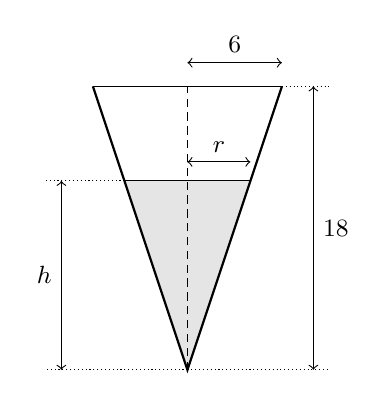
\begin{tikzpicture}[x=0.2cm,y=0.2cm,font=\small]
\fill[gray!20] (0,0)--(-4,12)--(4,12)--cycle;
\draw[thick] (-6,18)--(0,0)--(6,18);
\draw (-6,18)--(6,18);
\draw (-4,12)--(4,12);
\draw[densely dashed] (0,0)--(0,18);
\draw[densely dotted] (0,0)--(9,0) (6,18)--(9,18) (0,0)--(-9,0) (-4,12)--(-9,12);
\draw[<->] (8,0)--(8,18) node[midway,right] {$18$};
\draw[<->] (-8,0)--(-8,12) node[midway,left] {$h$};
\draw[<->] (0,19.5)--(6,19.5) node[midway,above] {$6$};
\draw[<->] (0,13.2)--(4,13.2) node[midway,above] {$r$};
\end{tikzpicture}
\end{center}
\begin{cnsolution}
设溶液的总体积为 $k$, 则
\[
\frac{\pi h^3}{27}+25\pi H=k.
\]
两边对 $t$ 求导, $\displaystyle\frac{\pi h^2}9\cdot\frac{\dd h}{\dd t}+25\pi\frac{\dd H}{\dd t}=0$, 所以
\[
\frac{\dd H}{\dd t}=-\frac{h^2}{225}\cdot\frac{\dd h}{\dd t}.
\]
代入 $h=12$, $\displaystyle\frac{\dd h}{\dd t}=-1$, 得 $\displaystyle\frac{\dd H}{\dd t}=\frac{144}{225}=0.64$, 即筒中液面以 $0.64$ cm/min 的速度上升.
\end{cnsolution}
\begin{example}\label{ex:c2-h3-8}
\textnormal{(指定作业: 习题2.3第8题)} 球的半径以 $5$~cm/s 的速度匀速增长. 问当球的半径为 $50$~cm 时, 球的表面积和体积的增长速度是多少?
\end{example}
\begin{cnsolution}
设时刻 $t$ 球的半径为 $r$, 则表面积 $S=4\pi r^2$, 体积 $\displaystyle V=\frac43\pi r^3$, 并且 $\displaystyle\frac{\dd r}{\dd t}=5$ cm/s. 两式两边对 $t$ 求导,
\[
\frac{\dd S}{\dd t}=8\pi r\frac{\dd r}{\dd t},\qquad\frac{\dd V}{\dd t}=4\pi r^2\frac{\dd r}{\dd t}.
\]
代入 $r=50$, $\displaystyle\frac{\dd r}{\dd t}=5$, 得表面积的增长速度为 $8\pi\cdot50\cdot5=2000\pi\approx6283$ cm$^2$/s, 体积的增长速度为 $4\pi\cdot50^2\cdot5=50000\pi\approx1.571\times10^5$ cm$^3$/s.
\end{cnsolution}
\begin{example}\label{ex:c2-h3-10}
\textnormal{(选自教材习题2.3第10题)} 半径为 $a$ 的球以速度 $c$ 匀速沉入半径为 $b$ ($b>a$) 的圆柱形容器的水中. 证明球浸没一半时, 水面上升的速度为 $\displaystyle\frac{a^2c}{b^2-a^2}$.
\end{example}
\par\indent\textbf{分析:} 设时刻 $t$ 水面的高度为 $H$, 要求 $\displaystyle\frac{\dd H}{\dd t}$. 球以速度 $c$ 下沉, 水面随之上升, 两者通过体积联系起来. 水的体积不变, 而水面以下的总体积 $\pi b^2H$ 等于水的体积加上球浸入部分的体积. 设球浸入水中的深度为 $s$, 浸入部分是高为 $s$ 的球缺, 即球被平面截下的部分. 由球缺的体积公式, 它的体积为 $\displaystyle\pi s^2\left(a-\frac s3\right)$ ($0\le s\le2a$); 这个公式可由祖暅原理推出, 以后讲定积分的应用时还会再推导.

体积的等式两边对 $t$ 求导, 会出现 $\displaystyle\frac{\dd s}{\dd t}$. 它不等于 $c$, 因为水面上升和球的下沉都使 $s$ 增加. 设球的最低点离容器底的高度为 $p$, 则 $\displaystyle\frac{\dd p}{\dd t}=-c$. 下图是过容器轴的截面, 阴影部分是水, 画的是 $a=1$, $b=2$, $p=1.4$, $H=2.2$ 的情形. 水面的高度 $H$ 等于 $p$ 加上浸入深度 $s$, 图中 $s=0.8$. 由 $s=H-p$ 得 $\displaystyle\frac{\dd s}{\dd t}=\frac{\dd H}{\dd t}-\frac{\dd p}{\dd t}=\frac{\dd H}{\dd t}+c$. 求导后代入 $s=a$, 就得到关于 $\displaystyle\frac{\dd H}{\dd t}$ 的方程.
\begin{center}
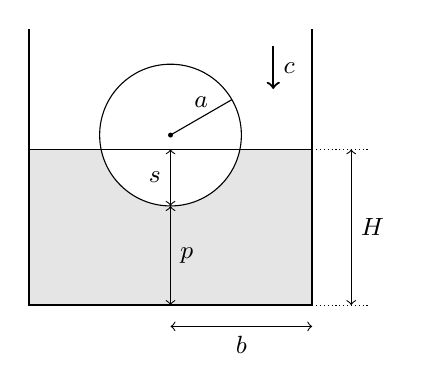
\begin{tikzpicture}[scale=0.9,font=\small]
\fill[gray!20] (-2,0) rectangle (2,2.2);
\fill[white] (0,2.4) circle (1);
\draw (0,2.4) circle (1);
\draw[thick] (-2,3.9)--(-2,0)--(2,0)--(2,3.9);
\draw (-2,2.2)--(2,2.2);
\draw[densely dotted] (2,2.2)--(2.8,2.2) (2,0)--(2.8,0);
\draw[<->] (2.55,0)--(2.55,2.2) node[midway,right] {$H$};
\draw[<->] (0,0)--(0,1.4) node[midway,right] {$p$};
\draw[<->] (0,1.4)--(0,2.2) node[midway,left] {$s$};
\fill (0,2.4) circle (1pt);
\draw (0,2.4)--({cos(30)},{2.4+sin(30)}) node[midway,above] {$a$};
\draw[<->] (0,-0.3)--(2,-0.3) node[midway,below] {$b$};
\draw[->,thick] (1.45,3.65)--(1.45,3.05) node[midway,right] {$c$};
\end{tikzpicture}
\end{center}
\begin{cnproof}
设水的体积为 $W$, 则
\[
\pi b^2H=W+\pi s^2\left(a-\frac s3\right),\qquad s=H-p.
\]
两边对 $t$ 求导, 由 $\displaystyle\frac{\dd}{\dd s}\left[\pi s^2\left(a-\frac s3\right)\right]=\pi(2as-s^2)$ 及链式法则,
\[
\pi b^2\frac{\dd H}{\dd t}=\pi(2as-s^2)\left(\frac{\dd H}{\dd t}-\frac{\dd p}{\dd t}\right)=\pi(2as-s^2)\left(\frac{\dd H}{\dd t}+c\right).
\]
球浸没一半时 $s=a$, $2as-s^2=a^2$, 于是 $\displaystyle b^2\frac{\dd H}{\dd t}=a^2\left(\frac{\dd H}{\dd t}+c\right)$, 所以 $\displaystyle\frac{\dd H}{\dd t}=\frac{a^2c}{b^2-a^2}$.
\end{cnproof}

证明中的因子 $\pi(2as-s^2)$ 恰好是球在水面处的截面面积. 水面到球心的距离是 $|a-s|$, 所以这个截面是半径为 $\sqrt{a^2-(a-s)^2}$ 的圆, 面积为 $\pi\bigl(a^2-(a-s)^2\bigr)=\pi(2as-s^2)$. 浸入深度增加 $\Delta s$ 时, 浸入部分多出的是水面处厚为 $\Delta s$ 的一薄层, 体积近似等于截面面积乘以 $\Delta s$. 所以水面以下体积的增加率等于这个截面面积乘以浸入深度的增加率, 这就是求导所得的等式.
\par\indent\textbf{方法小结:} 求相关变化率, 先设出随时间变化的各个量, 用几何或物理关系写出它们之间的等式; 等式两边对 $t$ 求导, 得到变化率之间的关系; 再代入指定时刻各量的值和已知的变化率. 要先求导再代值. 如果先代入数值, 变量就成了常数, 求导后得不到变化率之间的关系. 一个量同时随几个量变化时 (如浸入深度 $s=H-p$), 先用这几个量把它表示出来再求导. “下降”“减小”对应负的导数, 代入时要注意符号.
\section{高阶导数}
变速直线运动的速度 $v(t)=s'(t)$ 也随时间变化, 速度对时间的变化率是加速度 $a(t)=v'(t)$, 所以加速度是位置函数的导数的导数. 一般地, 导函数若仍可导, 可以对它再求导, 由此得到高阶导数.
\subsection{高阶导数的概念}
\begin{definitionsingle}
设函数 $y=f(x)$ 在点 $x$ 的某个邻域内可导. 若导函数 $f'$ 在点 $x$ 可导, 则称 $f$ 在 $x$ 处\textbf{二阶可导}, 并称 $f'$ 在 $x$ 处的导数
\[
f''(x)=\lim_{\Delta x\to0}\frac{f'(x+\Delta x)-f'(x)}{\Delta x}
\]
为 $f$ 在 $x$ 处的\textbf{二阶导数}, 也记作 $y''$, $\displaystyle\frac{\dd^2y}{\dd x^2}$ 或 $\displaystyle\frac{\dd^2f}{\dd x^2}$. 一般地, 设 $f$ 的 $n-1$ 阶导数 $f^{(n-1)}$ 在 $x$ 的某个邻域内存在, 若它在 $x$ 处可导, 则称其导数
\[
f^{(n)}(x)=\lim_{\Delta x\to0}\frac{f^{(n-1)}(x+\Delta x)-f^{(n-1)}(x)}{\Delta x}
\]
为 $f$ 在 $x$ 处的 \textbf{$n$ 阶导数}, 并称 $f$ 在 $x$ 处 \textbf{$n$ 阶可导}. $n$ 阶导数也记作 $y^{(n)}$, $\displaystyle\frac{\dd^ny}{\dd x^n}$ 或 $\displaystyle\frac{\dd^nf}{\dd x^n}$. 若 $f$ 在开区间 $I$ 内每一点 $n$ 阶可导, 则称 $f$ 在 $I$ 内 $n$ 阶可导.
\end{definitionsingle}
定义要求 $f$ 在 $x$ 的某个邻域内可导, 因为 $f'$ 在 $x$ 处的差商要用到 $f'$ 在 $x$ 附近的值. 二阶及二阶以上的导数统称\textbf{高阶导数}; 相应地, $f'$ 称为一阶导数, 并约定 $f^{(0)}=f$, $f^{(1)}=f'$. 三阶导数也记作 $f'''(x)$, $y'''$; 记号 $\displaystyle\frac{\dd^2y}{\dd x^2}$ 表示 $\displaystyle\frac{\dd}{\dd x}\left(\frac{\dd y}{\dd x}\right)$. $f^{(n)}$ 表示 $n$ 阶导数, 与 $n$ 次幂 $f^n$ 不同; $y''$ 也不同于 $(y')^2$.

二阶导数是一阶导数的变化率. 物理上, 本节开头的加速度就是位置函数的二阶导数, $a(t)=s''(t)$; 几何上, $f''(x)$ 是曲线 $y=f(x)$ 的切线斜率随 $x$ 的变化率. 按定义, 求高阶导数就是逐阶求导, 前面各节的法则和公式都可以使用. 例如由和、差与常数倍的法则, 可知和、差的 $n$ 阶导数等于 $n$ 阶导数的和、差, 常数因子可以提出.
\begin{example}\label{ex:c2-h4-1a}
\textnormal{(指定作业: 习题2.4第1题(4))} 设 $y=\sin\bigl[f(x^2)\bigr]$, 其中 $f$ 具有二阶导数. 求 $y''$.
\end{example}
\begin{cnsolution}
$y$ 是三层复合函数, 由外向内依次是正弦、$f$ 和 $x^2$. 由链式法则,
\[
y'=\cos\bigl[f(x^2)\bigr]\cdot f'(x^2)\cdot2x.
\]
$y'$ 是 $\cos\bigl[f(x^2)\bigr]$ 与 $2xf'(x^2)$ 的乘积, 再求导时用乘积法则. 第一个因子用链式法则求导; 第二个因子本身也是乘积, 求导时要用到 $\bigl[f'(x^2)\bigr]'=2xf''(x^2)$. 两个因子的导数分别是
\[
\Bigl(\cos\bigl[f(x^2)\bigr]\Bigr)'=-\sin\bigl[f(x^2)\bigr]\cdot2xf'(x^2),\qquad\bigl(2xf'(x^2)\bigr)'=2f'(x^2)+4x^2f''(x^2).
\]
所以
\[
y''=-4x^2\bigl[f'(x^2)\bigr]^2\sin\bigl[f(x^2)\bigr]+\bigl[2f'(x^2)+4x^2f''(x^2)\bigr]\cos\bigl[f(x^2)\bigr].
\]
\end{cnsolution}
\subsection{\texorpdfstring{几个常用的 $n$ 阶导数公式}{几个常用的 n 阶导数公式}}
\begin{example}\label{ex:c2-4-1}
\textnormal{(教材例4.1)} 证明下列 $n$ 阶导数公式 ($n\in\mathbb N^+$):

(1) $(a^x)^{(n)}=a^x(\ln a)^n$ ($a>0$, $a\ne1$), 特别地 $(e^x)^{(n)}=e^x$;

(2) $\displaystyle(\sin x)^{(n)}=\sin\left(x+\frac{n\pi}2\right)$;

(3) $\displaystyle(\cos x)^{(n)}=\cos\left(x+\frac{n\pi}2\right)$;

(4) $\displaystyle\bigl[\log_a(1+x)\bigr]^{(n)}=\frac{(-1)^{n-1}(n-1)!}{(1+x)^n\ln a}$, 特别地 $\displaystyle\bigl[\ln(1+x)\bigr]^{(n)}=\frac{(-1)^{n-1}(n-1)!}{(1+x)^n}$ ($a>0$, $a\ne1$, $x>-1$);

(5) $\bigl[(1+x)^\alpha\bigr]^{(n)}=\alpha(\alpha-1)\cdots(\alpha-n+1)(1+x)^{\alpha-n}$ ($\alpha\in\mathbb R$, $x>-1$).
\end{example}
\par\indent\textbf{分析:} 先求出前几阶导数找规律, 再用数学归纳法证明. 指数函数每求一次导数多出一个因子 $\ln a$. 正弦的一至四阶导数依次是
\[
\cos x,\qquad-\sin x,\qquad-\cos x,\qquad\sin x,
\]
四个一循环, 函数名和符号都在变, 不便用一个式子表示. 对任意常数 $c$, $\displaystyle\bigl[\sin(x+c)\bigr]'=\cos(x+c)=\sin\left(x+c+\frac\pi2\right)$, 所以每求一次导数, 结果仍是正弦, 只是自变量加上 $\displaystyle\frac\pi2$, 求 $n$ 次就加上 $\displaystyle\frac{n\pi}2$; 余弦也是这样. $(1+x)^\alpha$ 的前两阶导数是 $\alpha(1+x)^{\alpha-1}$ 与 $\alpha(\alpha-1)(1+x)^{\alpha-2}$. 每求一次导数, 当前的指数乘到系数上, 指数再减 $1$; 第 $k$ 次求导乘上的因子是 $\alpha-k+1$, 因此 $n$ 阶导数的系数是 $\alpha(\alpha-1)\cdots(\alpha-n+1)$. $\ln(1+x)$ 的一阶导数是 $(1+x)^{-1}$, 以后各阶就是 (5) 中 $\alpha=-1$ 的情形, 所以先证 (5), 再证 (4).
\begin{cnproof}
(1) $(a^x)'=a^x\ln a$. 若 $(a^x)^{(k)}=a^x(\ln a)^k$, 则 $(a^x)^{(k+1)}=(\ln a)^k(a^x)'=a^x(\ln a)^{k+1}$. 由数学归纳法, (1) 成立.

(2) $\displaystyle(\sin x)'=\cos x=\sin\left(x+\frac\pi2\right)$. 若 $\displaystyle(\sin x)^{(k)}=\sin\left(x+\frac{k\pi}2\right)$, 由链式法则,
\[
(\sin x)^{(k+1)}=\cos\left(x+\frac{k\pi}2\right)=\sin\left(x+\frac{k\pi}2+\frac\pi2\right)=\sin\left(x+\frac{(k+1)\pi}2\right).
\]

(3) $\displaystyle(\cos x)'=-\sin x=\cos\left(x+\frac\pi2\right)$. 若 $\displaystyle(\cos x)^{(k)}=\cos\left(x+\frac{k\pi}2\right)$, 则
\[
(\cos x)^{(k+1)}=-\sin\left(x+\frac{k\pi}2\right)=\cos\left(x+\frac{(k+1)\pi}2\right).
\]

(5) $\bigl[(1+x)^\alpha\bigr]'=\alpha(1+x)^{\alpha-1}$. 若 $\bigl[(1+x)^\alpha\bigr]^{(k)}=\alpha(\alpha-1)\cdots(\alpha-k+1)(1+x)^{\alpha-k}$, 则由链式法则
\[
\bigl[(1+x)^\alpha\bigr]^{(k+1)}=\alpha(\alpha-1)\cdots(\alpha-k+1)\cdot(\alpha-k)(1+x)^{\alpha-k-1},
\]
这就是 $n=k+1$ 时的公式.

(4) $\displaystyle\bigl[\ln(1+x)\bigr]'=(1+x)^{-1}$. 对 $n\ge2$, 由 (5) ($\alpha=-1$, 求 $n-1$ 阶导数),
\[
\bigl[\ln(1+x)\bigr]^{(n)}=\bigl[(1+x)^{-1}\bigr]^{(n-1)}=(-1)(-2)\cdots\bigl(-(n-1)\bigr)(1+x)^{-n}=\frac{(-1)^{n-1}(n-1)!}{(1+x)^n};
\]
$n=1$ 时公式也成立 ($0!=1$). 再由 $\displaystyle\log_a(1+x)=\frac{\ln(1+x)}{\ln a}$ 得一般的情形.
\end{cnproof}
当 $\alpha$ 是正整数 $m$ 时, (5) 中取 $n=m$ 得 $\bigl[(1+x)^m\bigr]^{(m)}=m!$; $n>m$ 时系数中出现因子 $\alpha-m=0$, 导数为零. 由此可以猜想, $m$ 次多项式的 $m+1$ 阶及更高阶导数都是零. 不过多项式在整个数轴上有定义, 而 (5) 只对 $x>-1$ 证明过, 2.1 节例\ref{ex:c2-1-7} 的公式 $(x^\mu)'=\mu x^{\mu-1}$ 也不包括 $x=0$, 所以还要说明正整数次幂的公式 $(x^j)'=jx^{j-1}$ 在 $x=0$ 处也成立. $x^j$ 在 $0$ 处的差商为 $\displaystyle\frac{(\Delta x)^j}{\Delta x}=(\Delta x)^{j-1}$, $j=1$ 时恒为 $1$, $j\ge2$ 时趋于 $0$, 都等于 $jx^{j-1}$ 在 $x=0$ 处的值. 因此 $(x^j)'=jx^{j-1}$ 对一切 $x$ 成立, 逐次求导得 $(x^j)^{(j)}=j!$, 更高阶的导数为零. 于是 $m$ 次多项式的 $m+1$ 阶及更高阶导数在整个数轴上都是零.

把例\ref{ex:c2-4-1} 中函数的自变量 $x$ 换成 $cx+d$ 后, $n$ 阶导数也容易求出. 设 $f$ 在区间 $I$ 内 $n$ 阶可导, $c,d$ 是常数. 当 $cx+d\in I$ 时, 由链式法则, $\bigl[f(cx+d)\bigr]'=cf'(cx+d)$, 归纳得\textbf{线性代换的 $n$ 阶导数公式}
\[
\bigl[f(cx+d)\bigr]^{(n)}=c^nf^{(n)}(cx+d).
\]
例如 $\displaystyle(\sin2x)^{(n)}=2^n\sin\left(2x+\frac{n\pi}2\right)$. 再如 $\displaystyle\frac1{1-x}$ 是把 $(1+u)^{-1}$ 中的 $u$ 换成 $-x$ 得到的. 由 (5) 取 $\alpha=-1$, $\bigl[(1+u)^{-1}\bigr]^{(n)}=(-1)(-2)\cdots(-n)(1+u)^{-n-1}=(-1)^nn!\,(1+u)^{-n-1}$, 再在线性代换的公式中取 $c=-1$, $d=0$, 得
\[
\left(\frac1{1-x}\right)^{(n)}=(-1)^n\cdot(-1)^nn!\,(1-x)^{-n-1}=\frac{n!}{(1-x)^{n+1}}\quad(x<1).
\]
\begin{example}\label{ex:c2-h4-1}
\textnormal{(指定作业: 习题2.4第1题(5)(6)(7))} 求 $n$ 阶导数: (5) $y=\sin^2x$; (6) $y=x\ln x$; (7) $\displaystyle y=\ln\frac{1+x}{1-x}$.
\end{example}
\begin{cnsolution}
(5) 由降幂公式, $\displaystyle\sin^2x=\frac12-\frac12\cos2x$. 对 $\cos2x$ 用例\ref{ex:c2-4-1}(3) 和线性代换的公式, 得
\[
y^{(n)}=-\frac12\cdot2^n\cos\left(2x+\frac{n\pi}2\right)=-2^{n-1}\cos\left(2x+\frac{n\pi}2\right).
\]

(6) 在 $x>0$ 时, $y'=\ln x+1$, $\displaystyle y''=\frac1x=x^{-1}$. 由 2.1 节例\ref{ex:c2-1-7} 逐次求导, $(x^{-1})^{(k)}=(-1)(-2)\cdots(-k)x^{-1-k}=(-1)^kk!\,x^{-k-1}$. 所以当 $n\ge2$ 时
\[
y^{(n)}=\bigl(x^{-1}\bigr)^{(n-2)}=\frac{(-1)^n(n-2)!}{x^{n-1}};
\]
$n=1$ 时 $y'=\ln x+1$.

(7) 由对数的运算法则, 在 $-1<x<1$ 时 $y=\ln(1+x)-\ln(1-x)$. 对 $\ln(1+u)$ 用线性代换的公式 ($c=-1$, $d=0$) 及例\ref{ex:c2-4-1}(4),
\[
\bigl[\ln(1-x)\bigr]^{(n)}=(-1)^n\cdot\frac{(-1)^{n-1}(n-1)!}{(1-x)^n}=-\frac{(n-1)!}{(1-x)^n},
\]
所以
\[
y^{(n)}=(n-1)!\left[\frac{(-1)^{n-1}}{(1+x)^n}+\frac1{(1-x)^n}\right].
\]
\end{cnsolution}
\subsection{莱布尼茨公式}
\begin{theoremsingle}[莱布尼茨公式]
设 $u,v$ 在开区间 $I$ 内 $n$ 阶可导, 则 $uv$ 在 $I$ 内 $n$ 阶可导, 并且
\[
(uv)^{(n)}=u^{(n)}v+C_n^1u^{(n-1)}v'+C_n^2u^{(n-2)}v''+\cdots+C_n^ku^{(n-k)}v^{(k)}+\cdots+uv^{(n)},
\]
其中 $\displaystyle C_n^k=\frac{n(n-1)\cdots(n-k+1)}{k!}$ 是组合数.
\end{theoremsingle}
\par\indent\textbf{分析:} 先看 $n=2$:
\[
(uv)''=(u'v+uv')'=(u''v+u'v')+(u'v'+uv'')=u''v+2u'v'+uv'',
\]
系数 $1,2,1$ 与 $(a+b)^2$ 展开式的系数相同. 这是因为按乘积法则 $(uv)'=u'v+uv'$, 每求一次导数, 每一项都分成两项, 一项中 $u$ 多求一次导数, 另一项中 $v$ 多求一次导数. 求 $n$ 次导数时, 每一次都要选择对 $u$ 求导还是对 $v$ 求导; 恰有 $k$ 次对 $v$ 求导的选法有 $C_n^k$ 种, 每种选法得到一项 $u^{(n-k)}v^{(k)}$, 所以 $u^{(n-k)}v^{(k)}$ 的系数是 $C_n^k$. 二项式定理中 $a^{n-k}b^k$ 的系数也是这样得到的. 证明用数学归纳法, 合并同类项时用组合数的性质 $C_n^{k-1}+C_n^k=C_{n+1}^k$.
\begin{cnproof}
$n=1$ 时就是乘积的求导法则. 设公式对 $n$ 成立, 并设 $u,v$ 在 $I$ 内 $n+1$ 阶可导. $(uv)^{(n+1)}$ 是 $(uv)^{(n)}$ 的导数, 所以把公式右端逐项求导. 右端的一般项是 $C_n^ku^{(n-k)}v^{(k)}$ ($0\le k\le n$), 其中 $u^{(n-k)}$ 与 $v^{(k)}$ 都是不超过 $n$ 阶的导数, 还可以再求导. 由乘积法则
\[
\bigl(C_n^ku^{(n-k)}v^{(k)}\bigr)'=C_n^ku^{(n-k+1)}v^{(k)}+C_n^ku^{(n-k)}v^{(k+1)}.
\]
把右端各项都求导后, $u^{(n+1)}v$ 与 $uv^{(n+1)}$ 各出现一次, 系数为 $1=C_{n+1}^0=C_{n+1}^{n+1}$. 对 $1\le k\le n$, 含 $u^{(n+1-k)}v^{(k)}$ 的项有两个: 一个由 $C_n^ku^{(n-k)}v^{(k)}$ 中的 $u^{(n-k)}$ 求导得到, 另一个由 $C_n^{k-1}u^{(n-k+1)}v^{(k-1)}$ 中的 $v^{(k-1)}$ 求导得到. 两项的系数之和为 $C_n^k+C_n^{k-1}=C_{n+1}^k$. 所以
\[
(uv)^{(n+1)}=u^{(n+1)}v+C_{n+1}^1u^{(n)}v'+\cdots+C_{n+1}^ku^{(n+1-k)}v^{(k)}+\cdots+uv^{(n+1)},
\]
公式对 $n+1$ 成立.
\end{cnproof}
\begin{example}\label{ex:c2-4-2}
\textnormal{(教材例4.2)} 设 $y=x^2\sin x$, 求 $y^{(100)}$.
\end{example}
\begin{cnsolution}
$x^2$ 的三阶及以上的导数都是零, $\sin x$ 的各阶导数由例\ref{ex:c2-4-1} 给出, 所以用莱布尼茨公式. 把多项式取作 $v$, 即 $u=\sin x$, $v=x^2$, 这时公式中含 $v'''$ 及更高阶导数的项都是零, 只剩前三项:
\[
\begin{aligned}
y^{(100)}&=(\sin x)^{(100)}\cdot x^2+C_{100}^1(\sin x)^{(99)}\cdot2x+C_{100}^2(\sin x)^{(98)}\cdot2\\
&=x^2\sin(x+50\pi)+200x\sin\left(x+\frac{99\pi}2\right)+9900\sin(x+49\pi)\\
&=x^2\sin x-200x\cos x-9900\sin x,
\end{aligned}
\]
其中 $\displaystyle\sin\left(x+\frac{99\pi}2\right)=\sin\left(x+\frac{3\pi}2\right)=-\cos x$, $\sin(x+49\pi)=\sin(x+\pi)=-\sin x$.
\end{cnsolution}
\begin{example}\label{ex:c2-h4-1b}
\textnormal{(指定作业: 习题2.4第1题(8))} 设 $y=x^2e^x$, 求 $y^{(100)}$.
\end{example}
\begin{cnsolution}
取 $u=e^x$, $v=x^2$, 用莱布尼茨公式. $(e^x)^{(k)}=e^x$, 而 $x^2$ 的三阶及以上的导数都是零, 只剩前三项:
\[
y^{(100)}=e^x\cdot x^2+C_{100}^1e^x\cdot2x+C_{100}^2e^x\cdot2=e^x(x^2+200x+9900).
\]
\end{cnsolution}
\begin{example}\label{ex:c2-h4-6}
\textnormal{(选自教材习题2.4第6题)} 设 $f(x)$ 是 $n$ 次多项式, $a$ 是 $f(x)=0$ 的 $k$ 重根 ($1\le k\le n$), 即 $f(x)=(x-a)^kg(x)$, 其中 $g$ 是多项式, $g(a)\ne0$. 证明
\[
f(a)=f'(a)=\cdots=f^{(k-1)}(a)=0,\qquad f^{(k)}(a)\ne0.
\]
\end{example}
\begin{cnproof}
$f$ 是 $(x-a)^k$ 与 $g$ 的乘积, 用莱布尼茨公式, 只需知道 $(x-a)^k$ 的各阶导数在 $a$ 处的值. 记 $u=(x-a)^k$. 由例\ref{ex:c2-4-1} 后的说明, $(x^k)'=kx^{k-1}$ 对一切 $x$ (包括 $x=0$) 成立, 逐次求导得 $(x^k)^{(j)}=k(k-1)\cdots(k-j+1)x^{k-j}$. 在线性代换的公式中取 $c=1$, $d=-a$, 得
\[
u^{(j)}=k(k-1)\cdots(k-j+1)(x-a)^{k-j}\quad(0\le j\le k),
\]
所以 $j<k$ 时 $u^{(j)}(a)=0$, 而 $u^{(k)}=k!$. 对 $0\le m\le k$, 由莱布尼茨公式, $f^{(m)}$ 是 $C_m^ju^{(j)}g^{(m-j)}$ ($0\le j\le m$) 这样的项之和. 若 $m\le k-1$, 每一项中 $j\le m<k$, 在 $x=a$ 处 $u^{(j)}(a)=0$, 所以 $f^{(m)}(a)=0$. 若 $m=k$, 在 $x=a$ 处只剩 $j=k$ 的一项, $f^{(k)}(a)=k!\,g(a)\ne0$.
\end{cnproof}
\par\indent\textbf{方法小结:} 求 $n$ 阶导数, 可以先求前几阶找规律, 再用数学归纳法证明. 也可以先用降幂公式、对数的运算法则等, 把函数化为 $e^x$, $\sin x$, $\cos x$, $(1+x)^\alpha$, $\ln(1+x)$ 的和、常数倍或线性代换 $f(cx+d)$, 再用例\ref{ex:c2-4-1} 的公式; 线性代换使 $n$ 阶导数多出因子 $c^n$, $c=-1$ 时不要漏掉符号 $(-1)^n$. 乘积中有一个因子是 $m$ 次多项式时用莱布尼茨公式, 把多项式取作 $v$, 只剩前 $m+1$ 项.
\subsection{隐函数、参数方程和反函数的二阶导数}
\begin{example}\label{ex:c2-4-3}
\textnormal{(教材例4.3)} 设方程 $x^2+xy+y^2=4$ 确定隐函数 $y=y(x)$, 求 $y''$, 并求 $x=0$ 时 $y''$ 的值.
\end{example}
\par\indent\textbf{分析:} 对方程求一次导数得到含 $y'$ 的等式, 其中 $y$ 与 $y'$ 都是 $x$ 的函数, 再对这个等式求导就得到含 $y''$ 的等式. 解出的 $y''$ 中含有 $y'$, 把 $y'$ 的表达式代入, $y''$ 就只用 $x$, $y$ 表示. 通分后若分子中出现 $x^2+xy+y^2$, 还可以用原方程把它换成 $4$.
\begin{cnsolution}
方程两边对 $x$ 求导,
\[
2x+y+xy'+2yy'=0,\qquad y'=-\frac{2x+y}{x+2y}\quad(x+2y\ne0).
\]
由 $x+2y\ne0$, $y'$ 是两个可导函数之商, 也可导. 把 $2x+y+xy'+2yy'=0$ 再对 $x$ 求导, $2+y'+y'+xy''+2(y')^2+2yy''=0$, 所以
\[
y''=-\frac{2\bigl(1+y'+(y')^2\bigr)}{x+2y}.
\]
把 $y'$ 代入 $1+y'+(y')^2$, 通分后分子为
\[
\begin{aligned}
&(x+2y)^2-(2x+y)(x+2y)+(2x+y)^2\\
&\qquad=(x^2+4xy+4y^2)-(2x^2+5xy+2y^2)+(4x^2+4xy+y^2)=3(x^2+xy+y^2),
\end{aligned}
\]
即 $\displaystyle1+y'+(y')^2=\frac{3(x^2+xy+y^2)}{(x+2y)^2}$. 再由原方程 $x^2+xy+y^2=4$,
\[
y''=-\frac{6(x^2+xy+y^2)}{(x+2y)^3}=-\frac{24}{(x+2y)^3}.
\]
$x=0$ 时 $y^2=4$, $y=\pm2$, 方程在 $x=0$ 附近确定两个隐函数. 对 $y=2$ 的那一个, $\displaystyle y''=-\frac{24}{64}=-\frac38$; 对 $y=-2$ 的那一个, $\displaystyle y''=\frac38$.
\end{cnsolution}
\begin{example}\label{ex:c2-h4-2}
\textnormal{(选自教材习题2.4第2题(2))} 设 $y=\tan(x+y)$ 确定隐函数 $y=y(x)$, 求 $y''$.
\end{example}
\begin{cnsolution}
两边对 $x$ 求导, $y'=\sec^2(x+y)\cdot(1+y')$. 由原方程, $\sec^2(x+y)=1+\tan^2(x+y)=1+y^2$, 于是 $y'=(1+y^2)(1+y')$, 即 $-y^2y'=1+y^2$. 右端不为零, 所以 $y\ne0$, 并且
\[
y'=-\frac{1+y^2}{y^2}=-1-\frac1{y^2}.
\]
用原方程把 $y'$ 化成只含 $y$ 的式子后, 再求导只需对 $y$ 用链式法则:
\[
y''=\frac2{y^3}\cdot y'=-\frac{2(1+y^2)}{y^5}.
\]
\end{cnsolution}
\begin{example}\label{ex:c2-h4-2b}
\textnormal{(指定作业: 习题2.4第2题(3))} 设 $e^{x+y}=xy$ 确定隐函数 $y=y(x)$, 求 $y''$.
\end{example}
\begin{cnsolution}
方程一边是乘积, 一边是指数, 两边取对数后都化为和. 由 $xy=e^{x+y}>0$, $x,y$ 都不为零, 并且 $\ln(xy)=\ln|x|+\ln|y|$, 所以取对数得 $\ln|x|+\ln|y|=x+y$. 两边对 $x$ 求导,
\[
\frac1x+\frac{y'}y=1+y',\qquad\text{即}\quad\frac{1-y}y\,y'=\frac{x-1}x.
\]
若某点处 $y=1$, 则左端为零, 从而 $x=1$; 但 $(1,1)$ 不满足原方程 ($e^2\ne1$). 所以 $y\ne1$, 并且
\[
y'=\frac{y(x-1)}{x(1-y)}.
\]
由 $x\ne0$, $y\ne1$, $y'$ 是可导函数之商, 也可导. 把 $\displaystyle\frac{1-y}y\,y'=\frac{x-1}x$ 再对 $x$ 求导. 左端是 $\displaystyle\frac1y-1$ 与 $y'$ 的乘积, $\displaystyle\left(\frac1y-1\right)'=-\frac{y'}{y^2}$; 右端 $\displaystyle\frac{x-1}x=1-\frac1x$ 的导数是 $\displaystyle\frac1{x^2}$. 于是
\[
\frac{1-y}y\,y''-\frac{(y')^2}{y^2}=\frac1{x^2},\qquad y''=\frac y{1-y}\left[\frac1{x^2}+\left(\frac{y'}y\right)^2\right].
\]
代入 $\displaystyle\frac{y'}y=\frac{x-1}{x(1-y)}$, 通分得
\[
y''=\frac y{1-y}\cdot\frac{(1-y)^2+(x-1)^2}{x^2(1-y)^2}=\frac{y\bigl[(x-1)^2+(y-1)^2\bigr]}{x^2(1-y)^3}.
\]
\end{cnsolution}
对参数方程 $x=\varphi(t)$, $y=\psi(t)$ ($t\in I$), 设 $\varphi,\psi$ 在区间 $I$ 内二阶可导, $\varphi$ 在 $I$ 内严格单调, 并且 $\varphi'(t)\ne0$ ($t\in I$). 由 2.3 节参数方程的求导法则, 对每个 $t\in I$, 在对应点处 $\displaystyle\frac{\dd y}{\dd x}=\frac{\psi'(t)}{\varphi'(t)}$. 于是 $x=\varphi(t)$ 与 $\displaystyle\frac{\dd y}{\dd x}=\frac{\psi'(t)}{\varphi'(t)}$ 又是一对参数方程, 它确定的函数就是 $\displaystyle\frac{\dd y}{\dd x}$, 这个函数对 $x$ 的导数是 $\displaystyle\frac{\dd^2y}{\dd x^2}$. 由商的求导法则, $\displaystyle\frac{\psi'(t)}{\varphi'(t)}$ 在 $I$ 内可导. 对这一对参数方程再用一次参数方程的求导法则, 即把法则中的 $\psi$ 换成 $\displaystyle\frac{\psi'}{\varphi'}$, 得
\[
\frac{\dd^2y}{\dd x^2}=\frac{\dd}{\dd t}\left(\frac{\psi'(t)}{\varphi'(t)}\right)\cdot\frac1{\varphi'(t)}=\frac{\psi''(t)\varphi'(t)-\psi'(t)\varphi''(t)}{\bigl[\varphi'(t)\bigr]^2}\cdot\frac1{\varphi'(t)}=\frac{\psi''(t)\varphi'(t)-\psi'(t)\varphi''(t)}{\bigl[\varphi'(t)\bigr]^3}.
\]
这个公式不必记忆, 只需记住求法. 一般地, 把 $n$ 阶导数看作 $t$ 的函数, 对 $t$ 求导, 再除以 $\displaystyle\frac{\dd x}{\dd t}$, 就得到 $n+1$ 阶导数:
\[
\frac{\dd^{n+1}y}{\dd x^{n+1}}=\frac{\dd}{\dd t}\left(\frac{\dd^ny}{\dd x^n}\right)\cdot\frac1{\varphi'(t)}.
\]
\begin{example}\label{ex:c2-4-4}
\textnormal{(教材例4.4)} 设 $x=a\cos t$, $y=b\sin t$ ($0<t<\pi$, $a,b>0$), 求 $\displaystyle\frac{\dd^2y}{\dd x^2}$ 与 $\displaystyle\frac{\dd^3y}{\dd x^3}$.
\end{example}
\begin{cnsolution}
$x=a\cos t$ 在 $(0,\pi)$ 上严格减少, $\displaystyle\frac{\dd x}{\dd t}=-a\sin t\ne0$. 逐阶求导:
\[
\begin{aligned}
\frac{\dd y}{\dd x}&=\frac{b\cos t}{-a\sin t}=-\frac ba\cot t,\\
\frac{\dd^2y}{\dd x^2}&=\frac{\dd}{\dd t}\left(-\frac ba\cot t\right)\cdot\frac1{-a\sin t}=\frac b{a\sin^2t}\cdot\frac1{-a\sin t}=-\frac b{a^2\sin^3t},\\
\frac{\dd^3y}{\dd x^3}&=\frac{\dd}{\dd t}\left(-\frac b{a^2\sin^3t}\right)\cdot\frac1{-a\sin t}=\frac{3b\cos t}{a^2\sin^4t}\cdot\frac1{-a\sin t}=-\frac{3b\cos t}{a^3\sin^5t}.
\end{aligned}
\]
若把 $\displaystyle\frac{\dd y}{\dd x}=\frac{b\cos t}{-a\sin t}$ 的分子、分母分别对 $t$ 求导, 得到的是 $\displaystyle\frac{-b\sin t}{-a\cos t}=\frac ba\tan t$, 与 $\displaystyle\frac{\dd^2y}{\dd x^2}=-\frac b{a^2\sin^3t}$ 不同.
\end{cnsolution}
\begin{example}\label{ex:c2-h4-3b}
\textnormal{(指定作业: 习题2.4第3题(2))} 设 $x=\ln(1+t^2)$, $y=t-\arctan t$, 求 $\displaystyle\frac{\dd^2y}{\dd x^2}$.
\end{example}
\begin{cnsolution}
由 2.3 节例\ref{ex:c2-h3-3}(4), $x=\ln(1+t^2)$ 在 $t>0$ 与 $t<0$ 时分别严格单调, $\displaystyle\frac{\dd x}{\dd t}=\frac{2t}{1+t^2}$ 只在 $t=0$ 处为零, 并且在 $t\ne0$ 处 $\displaystyle\frac{\dd y}{\dd x}=\frac t2$. 把 $\displaystyle\frac t2$ 对 $t$ 求导, 再除以 $\displaystyle\frac{\dd x}{\dd t}$:
\[
\frac{\dd^2y}{\dd x^2}=\frac{\dd}{\dd t}\left(\frac t2\right)\cdot\frac{1+t^2}{2t}=\frac{1+t^2}{4t}\quad(t\ne0).
\]
\end{cnsolution}
\begin{example}\label{ex:c2-h4-3}
\textnormal{(选自教材习题2.4第3题(3))} 设 $x=f'(t)$, $y=tf'(t)-f(t)$, 其中 $f$ 二阶可导, $f''(t)\ne0$, 并且 $f'$ 严格单调. 求 $\displaystyle\frac{\dd^2y}{\dd x^2}$.
\end{example}
\begin{cnsolution}
$\displaystyle\frac{\dd x}{\dd t}=f''(t)$, $\displaystyle\frac{\dd y}{\dd t}=f'(t)+tf''(t)-f'(t)=tf''(t)$, 所以 $\displaystyle\frac{\dd y}{\dd x}=t$. 二阶导数的公式要用到 $x$ 对 $t$ 的二阶导数 $f'''(t)$, 而这里只知道 $x=f'(t)$ 一阶可导, 不能套用. 但 $x=f'(t)$ 与 $\displaystyle\frac{\dd y}{\dd x}=t$ 也是一对参数方程, 对它直接用 2.3 节参数方程的求导法则:
\[
\frac{\dd^2y}{\dd x^2}=\frac{\dd}{\dd t}(t)\cdot\frac1{f''(t)}=\frac1{f''(t)}.
\]
\end{cnsolution}
\begin{example}\label{ex:c2-h4-4}
\textnormal{(指定作业: 习题2.4第4题)} 设 $y=y(x)$ 由
\[
x=3t^2+2t+3,\qquad e^y\sin t-y+1=0
\]
确定, 求 $\displaystyle\left.\frac{\dd^2y}{\dd x^2}\right|_{t=0}$.
\end{example}
\par\indent\textbf{分析:} $x$ 是 $t$ 的显函数, $y$ 由第二个方程确定为 $t$ 的隐函数, 两者通过参数 $t$ 联系, 所以按参数方程求导. $\displaystyle\frac{\dd y}{\dd x}$ 等于 $y$ 对 $t$ 的导数除以 $\displaystyle\frac{\dd x}{\dd t}=6t+2$; 求二阶导数时, 把 $\displaystyle\frac{\dd y}{\dd x}$ 再对 $t$ 求导, 然后除以 $6t+2$. 这要用到 $y$ 对 $t$ 的一阶和二阶导数, 它们由第二个方程用隐函数的求导方法得到. 题目只要求 $t=0$ 处的值, 所以 $y$ 对 $t$ 的一阶、二阶导数也只需算出 $t=0$ 处的值; 但求 $y$ 对 $t$ 的二阶导数时, 要对代值以前的等式求导, 不能先代值再求导.
\begin{cnsolution}
$t=0$ 时 $x=3$; 由 $e^y\sin0-y+1=0$ 得 $y=1$. $\displaystyle x=3t^2+2t+3=3\left(t+\frac13\right)^2+\frac83$ 在 $\displaystyle t>-\frac13$ 时严格增加, 并且 $\displaystyle\frac{\dd x}{\dd t}=6t+2>0$; $t=0$ 时 $\displaystyle\frac{\dd x}{\dd t}=2$.

把 $y$ 看作 $t$ 的函数, 下标 $t$ 表示对 $t$ 求导. 第二个方程两边对 $t$ 求导,
\[
e^yy'_t\sin t+e^y\cos t-y'_t=0.
\]
整理得 $(1-e^y\sin t)\,y'_t=e^y\cos t$. $t=0$ 时 $1-e^y\sin t=1$, 由连续性和保号性, 在 $t=0$ 附近 $1-e^y\sin t\ne0$, 所以 $\displaystyle y'_t=\frac{e^y\cos t}{1-e^y\sin t}$, 它是可导函数之商, 也可导. 代入 $t=0$, $y=1$, 得 $y'_t(0)=e$. 把第一次求导所得的等式再对 $t$ 求导,
\[
\bigl[e^y(y'_t)^2\sin t+e^yy''_t\sin t+e^yy'_t\cos t\bigr]+\bigl(e^yy'_t\cos t-e^y\sin t\bigr)-y''_t=0,
\]
代入 $t=0$, $y=1$, $y'_t(0)=e$, 得 $2e^2-y''_t(0)=0$, 即 $y''_t(0)=2e^2$. 最后
\[
\frac{\dd y}{\dd x}=\frac{y'_t}{6t+2},\qquad\frac{\dd^2y}{\dd x^2}=\frac{\dd}{\dd t}\left(\frac{y'_t}{6t+2}\right)\cdot\frac1{6t+2}=\frac{y''_t(6t+2)-6y'_t}{(6t+2)^3},
\]
代入 $t=0$:
\[
\left.\frac{\dd^2y}{\dd x^2}\right|_{t=0}=\frac{2e^2\cdot2-6e}{2^3}=\frac{2e^2-3e}4.
\]
\end{cnsolution}
\begin{example}\label{ex:c2-h4-7}
\textnormal{(选自教材习题2.4第7题)} 设 $f$ 在 $1$ 的某个邻域内严格单调且二阶可导, $g$ 是它的反函数, $f(1)=2$, $\displaystyle f'(1)=-\frac{\sqrt3}3$, $f''(1)=1$. 求 $g''(2)$.
\end{example}
\par\indent\textbf{分析:} 由反函数的求导法则, $\displaystyle g'(y)=\frac1{f'(x)}$, 其中 $x=g(y)$. 求 $g''$ 时, 要把这个式子对 $y$ 再求一次导数. 和参数方程的情形一样, 右端是用另一个变量 $x$ 表示的, 它通过 $x=g(y)$ 成为 $y$ 的复合函数. 由链式法则, 对 $y$ 求导等于对 $x$ 求导再乘以 $\displaystyle\frac{\dd x}{\dd y}=g'(y)$.
\begin{cnsolution}
$f'$ 在 $1$ 可导, 因而连续, 又 $f'(1)\ne0$, 由保号性, 在 $1$ 的某个邻域内 $f'(x)\ne0$. 由 2.2 节定理\ref{thm:c2-2-inv}, 在 $2$ 的某个邻域内 $\displaystyle g'(y)=\frac1{f'(g(y))}$. 再由倒数的求导公式和链式法则,
\[
g''(y)=-\frac{f''(g(y))\,g'(y)}{\bigl[f'(g(y))\bigr]^2}=-\frac{f''(x)}{\bigl[f'(x)\bigr]^3}\quad(x=g(y)).
\]
$y=2$ 对应 $x=1$, $\displaystyle\bigl[f'(1)\bigr]^3=-\frac{3\sqrt3}{27}=-\frac{\sqrt3}9$, 所以 $\displaystyle g''(2)=-\frac{f''(1)}{\bigl[f'(1)\bigr]^3}=\frac9{\sqrt3}=3\sqrt3$. 注意 $\displaystyle g'(2)=\frac1{f'(1)}$, 但 $g''(2)$ 不等于 $\displaystyle\frac1{f''(1)}=1$.
\end{cnsolution}
\begin{example}\label{ex:c2-h4-8}
\textnormal{(选自教材习题2.4第8题)} 设 $y=y(x)$ 在 $(-1,1)$ 内二阶可导, 并且满足
\[
(1-x^2)y''-xy'+a^2y=0.
\]
作变换 $x=\sin t$ ($\displaystyle|t|<\frac\pi2$), 证明 $y$ 作为 $t$ 的函数满足 $\displaystyle\frac{\dd^2y}{\dd t^2}+a^2y=0$.
\end{example}
\par\indent\textbf{分析:} $y$ 通过 $x=\sin t$ 成为 $t$ 的复合函数. 要把 $\displaystyle\frac{\dd^2y}{\dd t^2}$ 用 $y''$, $y'$ (对 $x$ 的导数) 表示出来, 再与已知方程比较. 第二次求导时, $y'(x)$ 也是 $t$ 的复合函数, 对 $t$ 求导要再乘以 $\displaystyle\frac{\dd x}{\dd t}=\cos t$.
\begin{cnproof}
由链式法则, $\displaystyle\frac{\dd y}{\dd t}=y'(x)\cos t$. 再对 $t$ 求导, 由乘积法则和链式法则,
\[
\frac{\dd^2y}{\dd t^2}=y''(x)\cos t\cdot\cos t-y'(x)\sin t=(1-x^2)y''-xy',
\]
其中用到 $\sin t=x$, $\cos^2t=1-x^2$. 由已知方程, 右端等于 $-a^2y$, 所以 $\displaystyle\frac{\dd^2y}{\dd t^2}+a^2y=0$.
\end{cnproof}
\par\indent\textbf{方法小结:} 隐函数、参数方程、反函数和变量代换的二阶导数, 都是对一阶导数的表达式再求导, 这个表达式中仍含有中间变量. 隐函数中 $y$ 与 $y'$ 都是 $x$ 的函数, 求出 $y''$ 后用 $y'$ 的表达式和原方程化简. 参数方程中对 $t$ 求导后要再除以 $\displaystyle\frac{\dd x}{\dd t}$, $\displaystyle\frac{\dd^2y}{\dd x^2}$ 一般不等于 $\displaystyle\frac{\psi''(t)}{\varphi''(t)}$. 反函数和变量代换中出现 $f'(g(y))$, $y'(\sin t)$ 这类复合函数, 再求导时要乘以内层函数的导数; 反函数的二阶导数也不是 $\displaystyle\frac1{f''(x)}$.
\section{微分}
导数刻画函数在一点的变化率. 实际问题中还常常需要估计自变量有微小改变 $\Delta x$ 时函数的改变量 $\Delta y$. $\Delta y$ 一般是 $\Delta x$ 的复杂函数. 但当函数可导时, $\Delta y$ 可以用一个与 $\Delta x$ 成正比的量近似代替, 并且 $\Delta x\to0$ 时误差与 $|\Delta x|$ 之比趋于零. 这个量就是微分.
\subsection{微分的概念}
先看两个例子. 正方形金属薄片受热膨胀, 边长从 $x_0$ 变到 $x_0+\Delta x$, 面积 $S=x^2$ 的增量为
\[
\Delta S=(x_0+\Delta x)^2-x_0^2=2x_0\Delta x+(\Delta x)^2.
\]
当 $\Delta x>0$ 时, 第一部分 $2x_0\Delta x$ 是薄片沿相邻两边增加的两个矩形的面积, 矩形的长为 $x_0$, 宽为 $\Delta x$; 第二部分 $(\Delta x)^2$ 是角上边长为 $\Delta x$ 的小正方形的面积. 第一部分与 $\Delta x$ 成正比, 是 $\Delta x$ 的线性函数; 第二部分在 $\Delta x\to0$ 时是比 $\Delta x$ 高阶的无穷小. 所以 $|\Delta x|$ 很小时 $\Delta S\approx2x_0\Delta x$. 同样, 球的半径从 $r$ 变到 $r+\Delta r$ 时, 体积 $\displaystyle V=\frac43\pi r^3$ 的增量为
\[
\Delta V=4\pi r^2\Delta r+4\pi r(\Delta r)^2+\frac43\pi(\Delta r)^3,
\]
后两项是比 $\Delta r$ 高阶的无穷小, 所以 $|\Delta r|$ 很小时 $\Delta V\approx4\pi r^2\Delta r$. 两个例子中线性部分的系数 $2x_0$ 与 $4\pi r^2$ 恰好是 $S'(x_0)$ 与 $V'(r)$.
\begin{definitionsingle}
设函数 $y=f(x)$ 在点 $x_0$ 的某个邻域内有定义. 若存在与 $\Delta x$ 无关的常数 $A$, 使
\[
\Delta y=f(x_0+\Delta x)-f(x_0)=A\Delta x+o(\Delta x)\quad(\Delta x\to0),
\]
则称 $f$ 在点 $x_0$ \textbf{可微}, 并称 $A\Delta x$ 为 $f$ 在点 $x_0$ 的\textbf{微分}, 记作 $\dd y\big|_{x=x_0}$ 或 $\dd f(x)\big|_{x=x_0}$, 即 $\dd y\big|_{x=x_0}=A\Delta x$.
\end{definitionsingle}
这里 $o(\Delta x)$ 表示比 $\Delta x$ 高阶的无穷小 (1.7 节). $f$ 在 $x_0$ 可微, 就是 $\Delta y$ 能像上面两个例子那样分成两部分: 一部分是 $\Delta x$ 的线性函数 $A\Delta x$, 另一部分是比 $\Delta x$ 高阶的无穷小. 微分是其中的前一部分. 系数 $A$ 必须与 $\Delta x$ 无关, 否则取 $\displaystyle A=\frac{\Delta y}{\Delta x}$ 就能使误差恒为零, 任何函数都可微了. $A$ 可以与 $x_0$ 有关, 例如正方形面积中 $A=2x_0$.

当 $A\ne0$ 时, 微分也称为增量的\textbf{线性主部}. 这是因为 $\displaystyle\frac{\Delta y}{\dd y}=\frac{A\Delta x+o(\Delta x)}{A\Delta x}=1+\frac{o(\Delta x)}{A\Delta x}\to1$, 即 $\Delta y\sim\dd y$. 按 1.7 节的定义, $\dd y$ 是 $\Delta y$ 关于 $\Delta x$ 的主部, 它又是 $\Delta x$ 的线性函数.
\begin{theoremsingle}[可微与可导的关系]
$f$ 在点 $x_0$ 可微的充分必要条件是 $f$ 在 $x_0$ 可导, 并且这时 $A=f'(x_0)$, 即 $\dd y\big|_{x=x_0}=f'(x_0)\Delta x$.
\end{theoremsingle}
\begin{cnproof}
对任一常数 $A$ 及 $\Delta x\ne0$, 有
\[
\frac{\Delta y-A\Delta x}{\Delta x}=\frac{\Delta y}{\Delta x}-A.
\]
所以 $\Delta x\to0$ 时, $\Delta y-A\Delta x=o(\Delta x)$ 当且仅当差商 $\displaystyle\frac{\Delta y}{\Delta x}\to A$. 若 $f$ 在 $x_0$ 可微, 差商就趋于定义中的常数 $A$, 所以 $f$ 在 $x_0$ 可导, 并且 $f'(x_0)=A$. 反过来, 若 $f$ 在 $x_0$ 可导, 取 $A=f'(x_0)$, 则差商趋于 $A$, 于是 $\Delta y=f'(x_0)\Delta x+o(\Delta x)$, 即 $f$ 在 $x_0$ 可微.
\end{cnproof}
可微与可导的定义不同, 但对一元函数两者等价, 因此常把可导也说成可微. 证明还说明, 满足定义的常数 $A$ 只能是 $f'(x_0)$, 所以微分是唯一确定的. 这要靠定义中误差比 $\Delta x$ 高阶的要求来保证. 如果只要求误差 $\Delta y-A\Delta x$ 趋于零, 那么 $f$ 在 $x_0$ 连续时 $\Delta y$ 与 $A\Delta x$ 都趋于零, 任何常数 $A$ 都满足这个要求, 微分就不唯一了.

定理中的 $\Delta x$ 也可以写成微分. 把自变量 $x$ 看作函数 $y=x$, 由 $(x)'=1$ 得 $\dd x=1\cdot\Delta x=\Delta x$, 即自变量的微分就是它的增量. 所以 $f$ 在区间上可导时, 它在每一点的微分为
\[
\dd y=f'(x)\,\dd x,\qquad\text{从而}\quad f'(x)=\frac{\dd y}{\dd x}\quad(\dd x\ne0).
\]
导数等于函数的微分与自变量的微分之商, 所以导数也称为\textbf{微商}; 记号 $\displaystyle\frac{\dd y}{\dd x}$ 现在可以看作分式.

微分也可以从变化率来理解. 假如函数在 $x_0$ 与 $x_0+\Delta x$ 之间一直按 $x_0$ 处的变化率 $f'(x_0)$ 均匀变化, 那么它的改变量就是 $f'(x_0)\Delta x$, 即微分 $\dd y$. 例如质点沿直线运动, 位置为 $s=s(t)$, 在时刻 $t_0$ 的速度为 $v(t_0)=s'(t_0)$. 用 $\dd s=v(t_0)\Delta t$ 代替 $\Delta s$, 相当于把从 $t_0$ 到 $t_0+\Delta t$ 的运动近似看作速度为 $v(t_0)$ 的匀速运动.

微分的几何意义见下图. 在曲线 $y=f(x)$ 上取点 $P(x_0,f(x_0))$ 与横坐标为 $x_0+\Delta x$ 的点 $Q$. 过 $P$ 作水平线, 过 $Q$ 作竖直线, 两线交于 $N$; 曲线在 $P$ 处的切线与直线 $NQ$ 交于 $M$. 那么 $PN=\Delta x$, $NQ=\Delta y$. 切线的斜率为 $f'(x_0)$, 所以 $NM=f'(x_0)\Delta x=\dd y$. 也就是说, $x$ 从 $x_0$ 变到 $x_0+\Delta x$ 时, 曲线纵坐标的增量是 $\Delta y$, 切线纵坐标的增量是 $\dd y$. 用 $\dd y$ 代替 $\Delta y$, 就是在 $P$ 附近用切线代替曲线, 误差 $MQ=\Delta y-\dd y$ 是比 $\Delta x$ 高阶的无穷小. 图中画的是 $f(x)=x^2$, $x_0=1$, $\Delta x=0.6$ 的情形. 这时 $\Delta y=1.6^2-1=1.56$, $\dd y=2\times0.6=1.2$, $MQ=0.36=(\Delta x)^2$, 是 $\dd y$ 的 $30\%$. 图中为了看清各条线段, $\Delta x$ 取得较大; 若 $\Delta x=0.1$, 则 $\dd y=0.2$, $MQ=0.01$, 只有 $\dd y$ 的 $5\%$.
\begin{center}
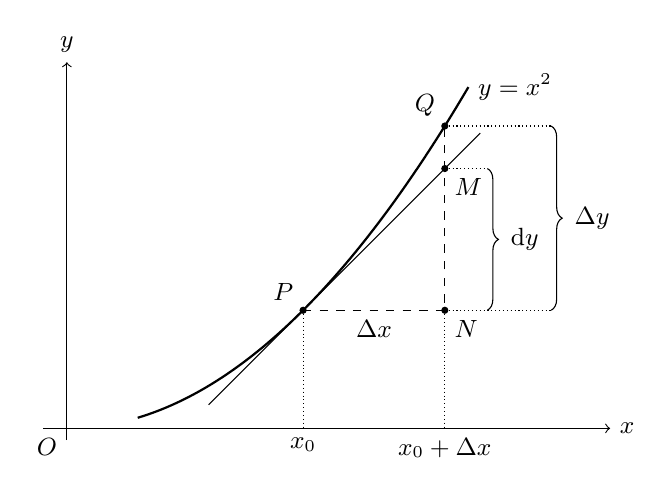
\begin{tikzpicture}[x=3cm,y=1.5cm,font=\small]
\draw[->] (-0.1,0)--(2.3,0) node[right] {$x$};
\draw[->] (0,-0.1)--(0,3.1) node[above] {$y$};
\draw[thick,domain=0.3:1.7,samples=60] plot (\x,{\x*\x});
\node[right] at (1.7,2.89) {$y=x^2$};
\draw (0.6,0.2)--(1.75,2.5);
\draw[dashed] (1,1)--(1.6,1)--(1.6,2.56);
\draw[densely dotted] (1.6,1)--(2.05,1);
\draw[densely dotted] (1.6,2.2)--(1.78,2.2);
\draw[densely dotted] (1.6,2.56)--(2.05,2.56);
\draw[decorate,decoration={brace,amplitude=4pt}] (1.78,2.2)--(1.78,1) node[midway,right=5pt] {$\dd y$};
\draw[decorate,decoration={brace,amplitude=4pt}] (2.05,2.56)--(2.05,1) node[midway,right=5pt] {$\Delta y$};
\fill (1,1) circle (1.3pt);
\fill (1.6,2.56) circle (1.3pt);
\fill (1.6,2.2) circle (1.3pt);
\fill (1.6,1) circle (1.3pt);
\node[above left] at (1,1) {$P$};
\node[above left] at (1.6,2.56) {$Q$};
\node[below right] at (1.6,2.2) {$M$};
\node[below right] at (1.6,1) {$N$};
\node[below] at (1.3,1) {$\Delta x$};
\draw[densely dotted] (1,1)--(1,0) node[below] {$x_0$};
\draw[densely dotted] (1.6,1)--(1.6,0) node[below] {$x_0+\Delta x$};
\node[below left] at (0,0) {$O$};
\end{tikzpicture}
\end{center}
\begin{example}\label{ex:c2-h5-1}
\textnormal{(选自教材习题2.5第1题)} 求函数 $y=5x+x^2$ 当 $x=2$, $\Delta x=0.001$ 时的增量 $\Delta y$ 与微分 $\dd y$.
\end{example}
\begin{cnsolution}
$\Delta y=\bigl[5(x+\Delta x)+(x+\Delta x)^2\bigr]-(5x+x^2)=(5+2x)\Delta x+(\Delta x)^2$. 由定义, $\dd y=(5+2x)\Delta x$, $\Delta y$ 与 $\dd y$ 恰好相差 $(\Delta x)^2$. 当 $x=2$, $\Delta x=0.001$ 时, $\dd y=9\times0.001=0.009$, $\Delta y=0.009+0.000001=0.009001$.
\end{cnsolution}
\begin{example}\label{ex:c2-h5-2}
\textnormal{(选自教材习题2.5第2题)} 判断下述说法是否正确: 若 $y=f(x)$ 在 $x_0$ 可导, 则当 $\Delta x\to0$ 时, $\dd y$ 是与 $\Delta x$ 同阶的无穷小.
\end{example}
\begin{cnsolution}
不正确. $\dd y=f'(x_0)\Delta x$. 若 $f'(x_0)\ne0$, 则 $\displaystyle\frac{\dd y}{\Delta x}=f'(x_0)\ne0$, $\dd y$ 与 $\Delta x$ 同阶; 若 $f'(x_0)=0$, 则 $\dd y\equiv0$, 比值的极限为 $0$, $\dd y$ 是比 $\Delta x$ 高阶的无穷小, 两者不同阶. 例如 $y=x^2$ 在 $x_0=0$ 处 $\dd y=0$. 所以说法只在 $f'(x_0)\ne0$ 时成立.
\end{cnsolution}
\subsection{微分的运算法则与一阶微分形式的不变性}
由 $\dd y=f'(x)\dd x$, 2.2 节导数公式表中的每个公式都给出一个微分公式 ($C$ 为常数):
\[
\begin{aligned}
&\dd C=0, &&\dd(x^\mu)=\mu x^{\mu-1}\dd x,\\
&\dd(a^x)=a^x\ln a\,\dd x, &&\dd(e^x)=e^x\dd x,\\
&\dd(\log_ax)=\frac{\dd x}{x\ln a}, &&\dd(\ln x)=\frac{\dd x}x,\\
&\dd(\sin x)=\cos x\,\dd x, &&\dd(\cos x)=-\sin x\,\dd x,\\
&\dd(\tan x)=\sec^2x\,\dd x, &&\dd(\cot x)=-\csc^2x\,\dd x,\\
&\dd(\sec x)=\sec x\tan x\,\dd x, &&\dd(\csc x)=-\csc x\cot x\,\dd x,\\
&\dd(\arcsin x)=\frac{\dd x}{\sqrt{1-x^2}}, &&\dd(\arccos x)=-\frac{\dd x}{\sqrt{1-x^2}},\\
&\dd(\arctan x)=\frac{\dd x}{1+x^2},\qquad &&\dd(\operatorname{arccot}x)=-\frac{\dd x}{1+x^2}.
\end{aligned}
\]
每个求导法则也给出一个微分法则: 设 $u,v$ 可导, 则
\[
\dd(u\pm v)=\dd u\pm\dd v,\qquad\dd(Cu)=C\,\dd u,\qquad\dd(uv)=v\,\dd u+u\,\dd v,\qquad\dd\left(\frac uv\right)=\frac{v\,\dd u-u\,\dd v}{v^2}\ (v\ne0).
\]
例如 $\dd(uv)=(uv)'\dd x=(u'v+uv')\dd x=v\,(u'\dd x)+u\,(v'\dd x)=v\,\dd u+u\,\dd v$, 其余各式同样由相应的求导法则乘以 $\dd x$ 得到.

设 $y=f(u)$ 可导. 若 $u$ 是自变量, 则 $\dd y=f'(u)\dd u$. 若 $u$ 是中间变量, 即 $u=\varphi(x)$ 是 $x$ 的可导函数, 则 $y=f(\varphi(x))$ 是自变量 $x$ 的函数, $\dd y$ 等于它对 $x$ 的导数乘 $\dd x$; 再由链式法则 (2.2 节定理\ref{thm:c2-2-chain}),
\[
\dd y=\bigl[f(\varphi(x))\bigr]'\dd x=f'(u)\varphi'(x)\dd x=f'(u)\,\dd u,
\]
其中第三个等号用到 $\dd u=\varphi'(x)\dd x$. 所以不论 $u$ 是自变量还是中间变量, 都有
\[
\dd y=f'(u)\,\dd u.
\]
这个性质称为\textbf{一阶微分形式的不变性}. 不变的是公式的形式, $\dd u$ 的含义并不相同. $u$ 是自变量时 $\dd u=\Delta u$; $u=\varphi(x)$ 是中间变量时 $\dd u=\varphi'(x)\Delta x$, 一般不等于 $\Delta u$. 例如 $u=x^2$, $x=1$, $\Delta x=0.1$ 时 $\dd u=0.2$, 而 $\Delta u=0.21$.

由一阶微分形式的不变性, 求复合函数的微分时可以把里层函数看作一个整体, 由外向内逐层求微分. 例如
\[
\dd\sin(5x+1)=\cos(5x+1)\,\dd(5x+1)=5\cos(5x+1)\,\dd x.
\]
\begin{example}\label{ex:c2-5-1}
\textnormal{(教材例5.1)} 设 $\displaystyle y=\frac{\sin2x}{x^2}$, 求 $\dd y$.
\end{example}
\begin{cnsolution}
$\dd(\sin2x)=2\cos2x\,\dd x$, $\dd(x^2)=2x\,\dd x$, 由商的微分法则, 当 $x\ne0$ 时
\[
\dd y=\frac{x^2\cdot2\cos2x\,\dd x-\sin2x\cdot2x\,\dd x}{x^4}=\frac{2(x\cos2x-\sin2x)}{x^3}\dd x.
\]
\end{cnsolution}
\begin{example}\label{ex:c2-5-2}
\textnormal{(教材例5.2)} 设 $y=e^{\sin^2x}$, 求 $\dd y$.
\end{example}
\begin{cnsolution}
由一阶微分形式的不变性逐层求微分,
\[
\dd y=e^{\sin^2x}\dd(\sin^2x)=e^{\sin^2x}\cdot2\sin x\,\dd(\sin x)=e^{\sin^2x}\cdot2\sin x\cos x\,\dd x=e^{\sin^2x}\sin2x\,\dd x.
\]
\end{cnsolution}
\begin{example}\label{ex:c2-h5-3}
\textnormal{(指定作业: 习题2.5第3题(4)(5))} 求下列函数的微分: (4) $y=x^{\sin x}$; (5) $y=\sin u$, $u=\ln(3x+1)$.
\end{example}
\begin{cnsolution}
(4) 2.3 节例\ref{ex:c2-3-4} 已用取对数求导法求出 $\displaystyle y'=x^{\sin x}\left(\cos x\ln x+\frac{\sin x}x\right)$ ($x>0$), 乘以 $\dd x$ 即得
\[
\dd y=x^{\sin x}\left(\cos x\ln x+\frac{\sin x}x\right)\dd x.
\]

(5) $u$ 是中间变量. 由一阶微分形式的不变性, 先对外层求微分, 再求 $\dd u$:
\[
\dd y=\cos u\,\dd u=\cos\bigl(\ln(3x+1)\bigr)\cdot\frac{3\,\dd x}{3x+1}=\frac{3\cos\bigl(\ln(3x+1)\bigr)}{3x+1}\dd x\quad\left(x>-\frac13\right).
\]
\end{cnsolution}
\begin{example}\label{ex:c2-5-3}
\textnormal{(教材例5.3)} 设方程 $x^2\sin y+xy^2=1$ 确定隐函数 $y=y(x)$, 求 $\dd y$.
\end{example}
\begin{cnsolution}
$y$ 是 $x$ 的函数, 由一阶微分形式的不变性, $\dd(\sin y)=\cos y\,\dd y$, 不必先求 $y'$. 方程两边求微分, 得
\[
2x\sin y\,\dd x+x^2\cos y\,\dd y+y^2\dd x+2xy\,\dd y=0,
\]
所以在 $x^2\cos y+2xy\ne0$ 处 $\displaystyle\dd y=-\frac{2x\sin y+y^2}{x^2\cos y+2xy}\dd x$.
\end{cnsolution}
\begin{example}\label{ex:c2-h5-5}
\textnormal{(指定作业: 习题2.5第5题(3))} 设方程 $\varphi(\sin x)+\sin\varphi(y)=\varphi(x+y)$ 确定隐函数 $y=y(x)$, 其中 $\varphi$ 处处可导. 求 $\dd y$.
\end{example}
\begin{cnsolution}
三项都是复合函数, 方程两边逐层求微分:
\[
\begin{aligned}
&\dd\varphi(\sin x)=\varphi'(\sin x)\cos x\,\dd x,\qquad\dd\sin\varphi(y)=\cos\varphi(y)\cdot\varphi'(y)\,\dd y,\\
&\dd\varphi(x+y)=\varphi'(x+y)\,(\dd x+\dd y).
\end{aligned}
\]
于是
\[
\varphi'(\sin x)\cos x\,\dd x+\cos\varphi(y)\,\varphi'(y)\,\dd y=\varphi'(x+y)(\dd x+\dd y).
\]
把含 $\dd y$ 的项移到一边, 在 $\cos\varphi(y)\,\varphi'(y)-\varphi'(x+y)\ne0$ 处
\[
\dd y=\frac{\varphi'(x+y)-\varphi'(\sin x)\cos x}{\cos\varphi(y)\,\varphi'(y)-\varphi'(x+y)}\dd x.
\]
\end{cnsolution}
\begin{example}\label{ex:c2-5-4}
\textnormal{(教材例5.4)} 求一个函数, 使它的微分等于 $\displaystyle\frac{\dd x}{x\cos^2\ln x}$.
\end{example}
\begin{cnsolution}
这是反过来使用微分公式. 分母中含有 $\ln x$ 的余弦, 而剩下的因子 $\displaystyle\frac{\dd x}x$ 恰好是 $\ln x$ 的微分. 把 $\ln x$ 看作一个整体 $u$, 所给的式子就成为 $\displaystyle\frac{\dd u}{\cos^2u}$, 它是 $\tan u$ 的微分. 由一阶微分形式的不变性,
\[
\frac{\dd x}{x\cos^2\ln x}=\frac{\dd(\ln x)}{\cos^2\ln x}=\dd\tan(\ln x),
\]
所以 $\tan(\ln x)$ 就是一个所求的函数; 它加上任意常数也是.
\end{cnsolution}
\begin{example}\label{ex:c2-h5-4}
\textnormal{(指定作业: 习题2.5第4题)} 在括号内填入适当的函数:
\[
\begin{aligned}
&\text{(1)}\ x\,\dd x=\dd(\quad);\quad\text{(2)}\ \frac1x\dd x=\dd(\quad);\quad\text{(3)}\ \sin x\,\dd x=\dd(\quad);\quad\text{(4)}\ \sec^2x\,\dd x=\dd(\quad);\\
&\text{(5)}\ \frac1{\sqrt x}\dd x=\dd(\quad);\quad\text{(6)}\ \frac{\dd x}{\sqrt{1-x^2}}=\dd(\quad);\quad\text{(7)}\ e^{-2x}\dd x=\dd(\quad);\\
&\text{(8)}\ x^2e^{-x^3}\dd x=(\quad)\,\dd(-x^3);\quad\text{(9)}\ \dd(\arctan e^{2x})=(\quad)\,\dd e^{2x};\\
&\text{(10)}\ \dd\bigl(\sin\sqrt{\cos x}\bigr)=(\quad)\,\dd\cos x.
\end{aligned}
\]
\end{example}
\begin{cnsolution}
(1)–(7) 都要找一个函数, 使它的导数等于 $\dd x$ 前的因子. 括号内分别填 (1) $\displaystyle\frac{x^2}2$; (2) $\ln|x|$ (2.2 节例\ref{ex:c2-2-10}); (3) $-\cos x$; (4) $\tan x$; (5) $2\sqrt x$; (6) $\arcsin x$; (7) $\displaystyle-\frac12e^{-2x}$. 这七个函数都可以再加任意常数 $C$.

(8) $\dd(-x^3)=-3x^2\dd x$, 所以 $\displaystyle x^2e^{-x^3}\dd x=-\frac13e^{-x^3}\dd(-x^3)$, 括号内填 $\displaystyle-\frac13e^{-x^3}$.

(9) 把 $e^{2x}$ 看作整体 $u$, $\displaystyle\dd(\arctan u)=\frac{\dd u}{1+u^2}$, 括号内填 $\displaystyle\frac1{1+e^{4x}}$.

(10) 把 $\cos x$ 看作整体 $u$, $\displaystyle\dd\bigl(\sin\sqrt u\bigr)=\cos\sqrt u\cdot\frac{\dd u}{2\sqrt u}$, 括号内填 $\displaystyle\frac{\cos\sqrt{\cos x}}{2\sqrt{\cos x}}$.
\end{cnsolution}
\begin{example}\label{ex:c2-h5-6}
\textnormal{(指定作业: 习题2.5第6题)} 求由参数方程 $x=3t^2+2t+3$, $e^y\sin t-y+1=0$ 所确定的函数 $y=f(x)$ 的微分 $\dd y$.
\end{example}
\begin{cnsolution}
先用 $\dd t$ 表示 $\dd y$ 与 $\dd x$, 再消去 $\dd t$. 第二个方程两边求微分, 其中 $\dd(e^y)=e^y\dd y$:
\[
e^y\sin t\,\dd y+e^y\cos t\,\dd t-\dd y=0,\qquad\dd y=\frac{e^y\cos t}{1-e^y\sin t}\dd t\quad(1-e^y\sin t\ne0).
\]
又 $\dd x=(6t+2)\dd t$. 由 $\displaystyle x=3\left(t+\frac13\right)^2+\frac83$ 可知, $x$ 在 $\displaystyle t>-\frac13$ 与 $\displaystyle t<-\frac13$ 时分别严格单调, 所以参数方程在这两个范围内各确定一个函数 $y=f(x)$. 在这两个范围内 $6t+2\ne0$, 因此 $t$ 是 $x$ 的可导函数, 把 $x$ 看作自变量时 $t$ 是中间变量. 由一阶微分形式的不变性, 用 $\dd t$ 表示 $\dd y$ 与 $\dd x$ 的两个式子仍然成立, 于是 $\displaystyle\dd t=\frac{\dd x}{6t+2}$. 代入 $\dd y$ 的式子, 得
\[
\dd y=\frac{e^y\cos t}{(6t+2)(1-e^y\sin t)}\dd x.
\]
$\dd x$ 的系数就是 $f'(x)$, 与 2.3 节参数方程的求导法则给出的结果相同.
\end{cnsolution}
\begin{example}\label{ex:c2-h5-7}
\textnormal{(选自教材习题2.5第7题)} 设 $f$ 二阶可导, $x=f(t)\cos t-f'(t)\sin t$, $y=f(t)\sin t+f'(t)\cos t$. 证明
\[
(\dd x)^2+(\dd y)^2=\bigl[f(t)+f''(t)\bigr]^2(\dd t)^2.
\]
\end{example}
\begin{cnproof}
用乘积的微分法则求 $\dd x$ 与 $\dd y$, 每个微分中含 $f'(t)$ 的两项互相抵消:
\[
\begin{aligned}
\dd x&=\bigl[f'(t)\cos t-f(t)\sin t-f''(t)\sin t-f'(t)\cos t\bigr]\dd t=-\bigl[f(t)+f''(t)\bigr]\sin t\,\dd t,\\
\dd y&=\bigl[f'(t)\sin t+f(t)\cos t+f''(t)\cos t-f'(t)\sin t\bigr]\dd t=\bigl[f(t)+f''(t)\bigr]\cos t\,\dd t.
\end{aligned}
\]
平方相加, 由 $\sin^2t+\cos^2t=1$ 即得所证等式.
\end{cnproof}
\subsection{微分在近似计算与误差估计中的应用}
由可微与可导的关系, 当 $f'(x_0)$ 存在时 $\Delta y=f'(x_0)\Delta x+o(\Delta x)$. 所以 $|\Delta x|$ 很小时 $\Delta y\approx\dd y$, 即
\[
f(x_0+\Delta x)\approx f(x_0)+f'(x_0)\Delta x,\qquad\text{或}\quad f(x)\approx f(x_0)+f'(x_0)(x-x_0).
\]
函数 $y=f(x_0)+f'(x_0)(x-x_0)$ 的图像是曲线在点 $(x_0,f(x_0))$ 处的切线, 所以这一近似就是用切线代替曲线. 当 $f(x_0)$ 与 $f'(x_0)$ 容易计算时, 可以用这个公式计算 $x_0$ 附近的函数值. 取 $x_0=0$, 得到 $|x|$ 很小时的近似公式 $f(x)\approx f(0)+f'(0)x$, 例如
\[
\sin x\approx x,\quad\tan x\approx x,\quad e^x\approx1+x,\quad\ln(1+x)\approx x,\quad(1+x)^\mu\approx1+\mu x,
\]
它们与 1.8 节列出的等价无穷小一致. 目前只知道误差是比 $\Delta x$ 高阶的无穷小, 还没有误差大小的定量估计.
\begin{example}\label{ex:c2-5-5}
\textnormal{(教材例5.5)} 求 $\sqrt[3]{995}$ 的近似值.
\end{example}
\begin{cnsolution}
离 $995$ 最近、立方根容易计算的数是 $1000$. 提出 $1000$ 后可以用 $(1+x)^\mu\approx1+\mu x$:
\[
\sqrt[3]{995}=10\left(1-\frac5{1000}\right)^{\frac13}\approx10\left(1-\frac13\cdot\frac5{1000}\right)=10-\frac1{60}\approx9.983.
\]
\end{cnsolution}
\begin{example}\label{ex:c2-5-6}
\textnormal{(教材例5.6)} 求 $\tan31^\circ$ 的近似值.
\end{example}
\begin{cnsolution}
$(\tan x)'=\sec^2x$ 是对以弧度为单位的 $x$ 而言的, 所以先把角化成弧度, $\displaystyle31^\circ=\frac\pi6+\frac\pi{180}$. 取 $\displaystyle x_0=\frac\pi6$, $\displaystyle\Delta x=\frac\pi{180}$, 由 $\displaystyle\tan\frac\pi6=\frac{\sqrt3}3$, $\displaystyle\sec^2\frac\pi6=\frac43$ 得
\[
\tan31^\circ\approx\frac{\sqrt3}3+\frac43\cdot\frac\pi{180}\approx0.577350+0.023271=0.600621.
\]
更精确的计算给出 $\tan31^\circ\approx0.60086$, 可见这个近似值只有前三位小数准确.
\end{cnsolution}
\begin{example}\label{ex:c2-h5-8}
\textnormal{(选自教材习题2.5第8题(2)(4))} 求近似值 (保留四位小数): (2) $\cos59^\circ$; (4) $e^{1.01}$.
\end{example}
\begin{cnsolution}
(2) $\displaystyle59^\circ=\frac\pi3-\frac\pi{180}$, 增量为负. 取 $\displaystyle x_0=\frac\pi3$, $\displaystyle\Delta x=-\frac\pi{180}$, 由 $(\cos x)'=-\sin x$,
\[
\cos59^\circ\approx\cos\frac\pi3-\sin\frac\pi3\cdot\left(-\frac\pi{180}\right)=\frac12+\frac{\sqrt3}2\cdot\frac\pi{180}\approx0.5+0.01511=0.51511\approx0.5151.
\]

(4) 取 $x_0=1$, $\Delta x=0.01$, 由 $(e^x)'=e^x$ 得 $e^{1.01}\approx e+e\times0.01=1.01e\approx2.7455$.
\end{cnsolution}

误差估计也用到微分. 设某个量的精确值为 $x$, 测量值为 $x_0$ ($x_0\ne0$). $|x-x_0|$ 称为\textbf{绝对误差}, $\displaystyle\frac{|x-x_0|}{|x_0|}$ 称为\textbf{相对误差}. 绝对误差通常无法确切知道, 但可以知道它不超过某个数 $\delta_x$; $\delta_x$ 称为\textbf{绝对误差限}, $\displaystyle\frac{\delta_x}{|x_0|}$ 称为\textbf{相对误差限}. 记 $\Delta x=x-x_0$, 则 $|\Delta x|\le\delta_x$. 若由公式 $y=f(x)$ 计算 $y$, 用 $y_0=f(x_0)$ 代替精确值 $f(x)$ 产生的误差为 $|\Delta y|=|f(x_0+\Delta x)-f(x_0)|$. 当 $\delta_x$ 很小时,
\[
|\Delta y|\approx|\dd y|=|f'(x_0)||\Delta x|\le|f'(x_0)|\,\delta_x,
\]
所以 $y$ 的绝对误差限约为 $\delta_y=|f'(x_0)|\delta_x$; 当 $y_0\ne0$ 时, 相对误差限约为 $\displaystyle\frac{\delta_y}{|y_0|}=\left|\frac{f'(x_0)}{f(x_0)}\right|\delta_x$, 常用百分数表示.
\begin{example}\label{ex:c2-5-7}
\textnormal{(教材例5.7)} 用游标卡尺测得圆钢的直径 $D=50.2$ mm, 绝对误差限 $\delta_D=0.05$ mm. 用公式 $\displaystyle S=\frac\pi4D^2$ 计算圆钢的截面积, 估计面积的绝对误差限与相对误差限.
\end{example}
\begin{cnsolution}
$\displaystyle S'(D)=\frac\pi2D$, 所以
\[
\delta_S=\frac\pi2D\,\delta_D=\frac\pi2\times50.2\times0.05\approx3.94\ (\text{mm}^2),\qquad\frac{\delta_S}S=\frac{\frac\pi2D\,\delta_D}{\frac\pi4D^2}=\frac{2\delta_D}D=\frac{0.1}{50.2}\approx0.2\%.
\]
\end{cnsolution}
\begin{example}\label{ex:c2-h5-12}
\textnormal{(选自教材习题2.5第12题)} 证明: 当半径的相对误差为 $1\%$ 时, 由半径算出的圆面积或球面积的相对误差约为 $2\%$.
\end{example}
\begin{cnproof}
设半径的测量值为 $r$, 误差为 $\Delta r$, 相对误差 $\displaystyle\frac{|\Delta r|}r=1\%$. 圆面积 $\pi r^2$ 与球面积 $4\pi r^2$ 都可以写成 $S=kr^2$ ($k>0$ 为常数). 由 $\dd S=2kr\,\Delta r$, 面积的相对误差
\[
\frac{|\Delta S|}S\approx\frac{|\dd S|}S=\frac{2kr|\Delta r|}{kr^2}=2\cdot\frac{|\Delta r|}r=2\times1\%=2\%.
\]
\end{cnproof}
\subsection{高阶微分}
设 $y=f(x)$ 二阶可导, $x$ 是自变量. 微分 $\dd y=f'(x)\dd x$ 仍是 $x$ 的函数, 其中 $\dd x=\Delta x$ 是事先取定的增量, 不随 $x$ 变化, 看作常数. $\dd y$ 的微分称为\textbf{二阶微分}:
\[
\dd^2y=\dd(\dd y)=\dd\bigl(f'(x)\dd x\bigr)=\bigl(f''(x)\dd x\bigr)\dd x=f''(x)\,\dd x^2,
\]
其中 $\dd x^2$ 表示 $(\dd x)^2$, 不要与 $\dd(x^2)=2x\,\dd x$ 混淆. 二阶微分也记作 $\dd^2f(x)$. 一般地, $n-1$ 阶微分的微分称为 \textbf{$n$ 阶微分}, 记作 $\dd^ny$ 或 $\dd^nf(x)$, 即 $\dd^ny=\dd(\dd^{n-1}y)$; 相应地, $\dd y$ 也称为\textbf{一阶微分}, 二阶及二阶以上的微分统称为\textbf{高阶微分}.

用数学归纳法可以证明, 只要 $f$ 有 $n$ 阶导数, 就有 $\dd^ny=f^{(n)}(x)\dd x^n$, 其中 $\dd x^n=(\dd x)^n$. $n=1$ 时这就是 $\dd y=f'(x)\dd x$. 设 $f$ 有 $n$ 阶导数, 并且 $\dd^{n-1}y=f^{(n-1)}(x)\dd x^{n-1}$, 则由 $\dd x$ 是常数,
\[
\dd^ny=\dd\bigl(f^{(n-1)}(x)\dd x^{n-1}\bigr)=\dd\bigl(f^{(n-1)}(x)\bigr)\dd x^{n-1}=f^{(n)}(x)\dd x^n.
\]
于是当 $\dd x\ne0$ 时 $\displaystyle f^{(n)}(x)=\frac{\dd^ny}{\dd x^n}$, 即 $x$ 是自变量时, $n$ 阶导数是 $n$ 阶微分与 $\dd x^n$ 之商, 这与 2.4 节高阶导数的记号一致.

高阶微分没有形式不变性. 设 $y=f(u)$ 与 $u=\varphi(x)$ 都二阶可导, $u$ 是中间变量, 这时 $\dd u=\varphi'(x)\dd x$ 一般随 $x$ 变化, 不能当作常数. 由一阶微分形式的不变性和乘积的微分法则,
\[
\dd^2y=\dd\bigl(f'(u)\dd u\bigr)=\dd\bigl(f'(u)\bigr)\,\dd u+f'(u)\,\dd(\dd u)=f''(u)\,\dd u^2+f'(u)\,\dd^2u,
\]
比 $u$ 为自变量时的 $f''(u)\dd u^2$ 多出一项 $f'(u)\dd^2u$. 当 $u$ 是 $x$ 的一次函数时 $\dd^2u=0$, 两式一致; 一般情形下多出的这一项不为零. 例如 $y=u^2$, $u=x^2$ 时, $\dd^2y=\dd^2(x^4)=12x^2\dd x^2$, 而 $f''(u)\dd u^2=2(2x\,\dd x)^2=8x^2\dd x^2$, 两者之差正是多出的一项 $f'(u)\dd^2u=2u\cdot2\,\dd x^2=4x^2\dd x^2$. 所以 $u$ 不是自变量时, $\displaystyle\frac{\dd^2y}{\dd u^2}$ 只表示 $y$ 对 $u$ 的二阶导数, 不能看作 $\dd^2y$ 与 $\dd u^2$ 之商. 在这个例子中, $y$ 对 $u$ 的二阶导数是 $2$, 而 $x\ne0$, $\dd x\ne0$ 时 $\dd^2y$ 与 $\dd u^2$ 之商是 $\displaystyle\frac{12x^2\dd x^2}{4x^2\dd x^2}=3$.
\begin{example}\label{ex:c2-h5-13}
\textnormal{(选自教材习题2.5第13题(2))} 设方程 $xy+y^2=1$ 确定隐函数 $y=y(x)$, 求 $\dd^2y$.
\end{example}
\begin{cnsolution}
$x$ 是自变量, 所以 $\dd^2y=y''\dd x^2$, 只需求出 $y''$. 求 $y''$ 的方法与 2.4 节例\ref{ex:c2-4-3} 相同. 方程两边对 $x$ 求导, 得 $y+xy'+2yy'=0$, 即 $y+(x+2y)y'=0$. 其中 $x+2y$ 不会为零, 因为 $x=-2y$ 时 $xy+y^2=-y^2\le0$, 不满足原方程. 所以
\[
y'=-\frac y{x+2y},
\]
它是两个可导函数之商, 也可导. 把 $y+(x+2y)y'=0$ 再对 $x$ 求导, 得 $y'+(1+2y')y'+(x+2y)y''=0$, 即 $2y'(1+y')+(x+2y)y''=0$, 所以
\[
y''=-\frac{2y'(1+y')}{x+2y}.
\]
把 $y'$ 与 $\displaystyle1+y'=\frac{x+y}{x+2y}$ 相乘, 并用原方程 $xy+y^2=1$, 得
\[
y'(1+y')=-\frac{y(x+y)}{(x+2y)^2}=-\frac{xy+y^2}{(x+2y)^2}=-\frac1{(x+2y)^2},
\]
于是 $\displaystyle y''=\frac2{(x+2y)^3}$, $\displaystyle\dd^2y=\frac{2\,\dd x^2}{(x+2y)^3}$.
\end{cnsolution}
\par\indent\textbf{方法小结:} 求微分可以先求导数再乘 $\dd x$, 也可以直接用微分法则和一阶微分形式的不变性, 由外向内逐层求微分. 隐函数可以对方程两边直接求微分. 反过来, 已知微分求函数时, 要把 $\dd x$ 前的因子与 $\dd x$ 凑成某个函数的微分. 用微分作近似计算时, 取一个靠近所求点的 $x_0$, 使 $f(x_0)$ 与 $f'(x_0)$ 都容易计算, 再用 $f(x_0+\Delta x)\approx f(x_0)+f'(x_0)\Delta x$; 三角函数中的角要化成弧度. 估计误差时, $y$ 的绝对误差限约为 $|f'(x_0)|\delta_x$. 求二阶微分时, 若 $x$ 是自变量, 先求 $y''$, 再乘 $\dd x^2$; 自变量的微分 $\dd x$ 是常数, 中间变量的微分 $\dd u$ 一般随 $x$ 变化, 不能当作常数.
\section{中值定理及函数的单调性、极值}
导数 $f'(x_0)$ 由 $x_0$ 附近的函数值决定, 描述的是函数在一点的局部性质; 单调性这类区间上的性质则涉及区间中任意两点的函数值. 要用导数研究区间上的性质, 例如由 $f'>0$ 推出 $f$ 单调增加, 就要用导数表示两点处的函数值之差 $f(x_2)-f(x_1)$. 微分中值定理给出了这样的表示. 证明中值定理要用到函数在一点的单调性和极值, 所以先讨论它们.
\subsection{函数在一点的单调性与极值}
第一章已经使用过单调函数, 这里给出正式的定义.
\begin{definition}
设 $f$ 在区间 $I$ 上有定义. 若对 $I$ 中任意两点 $x_1<x_2$ 都有 $f(x_1)\le f(x_2)$, 则称 $f$ 在 $I$ 上\textbf{单调增加}; 若都有 $f(x_1)<f(x_2)$, 则称 $f$ 在 $I$ 上\textbf{严格单调增加}. 把不等号反向, 就得到 (严格) \textbf{单调减少}的定义. 单调增加和单调减少的函数统称\textbf{单调函数}.
\end{definition}
\begin{definition}
设 $f$ 在 $x_0$ 的某个邻域内有定义. 若存在 $\delta>0$, 使当 $x_0-\delta<x<x_0$ 时 $f(x)\le f(x_0)$, 当 $x_0<x<x_0+\delta$ 时 $f(x)\ge f(x_0)$, 则称 $f$ 在点 $x_0$ \textbf{单调增加}; 若这两个不等式都是严格的, 则称 $f$ 在点 $x_0$ \textbf{严格单调增加}. 把不等号反向, 就得到 $f$ 在点 $x_0$ (严格) 单调减少的定义. (严格) 单调增加与 (严格) 单调减少统称在点 $x_0$ (严格) 单调.
\end{definition}
在一点单调增加, 只是把 $x_0$ 附近各点的函数值与 $f(x_0)$ 比较, 要求左侧的不超过它, 右侧的不小于它, 并不比较附近另外两点的函数值. 所以在一点单调增加不能推出在这一点的某个邻域内单调增加 (见本节定理\ref{thm:c2-6-mono} 后面的例子).
\begin{theorem}[导数的符号与一点的单调性]\label{thm:c2-6-point}
设 $f$ 在点 $x_0$ 可导. 若 $f'(x_0)>0$, 则 $f$ 在 $x_0$ 严格单调增加; 若 $f'(x_0)<0$, 则 $f$ 在 $x_0$ 严格单调减少.
\end{theorem}
\begin{cnproof}
设 $\displaystyle f'(x_0)=\lim_{x\to x_0}\frac{f(x)-f(x_0)}{x-x_0}>0$. 由保号性 (1.6 节定理1(4)), 存在 $\delta>0$, 使 $0<|x-x_0|<\delta$ 时 $\displaystyle\frac{f(x)-f(x_0)}{x-x_0}>0$, 即 $f(x)-f(x_0)$ 与 $x-x_0$ 同号. 于是 $x<x_0$ 时 $f(x)<f(x_0)$, $x>x_0$ 时 $f(x)>f(x_0)$, 所以 $f$ 在 $x_0$ 严格单调增加. $f'(x_0)<0$ 的情形同理.
\end{cnproof}
几何上, $f'(x_0)>0$ 表示切线的斜率为正, 这时在 $x_0$ 附近, 曲线上位于点 $(x_0,f(x_0))$ 左侧的点都比它低, 右侧的点都比它高. $f'(x_0)=0$ 时没有确定的结论. $x^3$ 与 $x^2$ 在 $0$ 的导数都是零, 但 $x^3$ 在 $0$ 严格单调增加, $x^2$ 在 $0$ 既不单调增加也不单调减少.

反过来, 若 $f$ 在 $x_0$ 可导并且在 $x_0$ 单调减少, 则在 $x_0$ 的某个去心邻域内差商 $\displaystyle\frac{f(x)-f(x_0)}{x-x_0}\le0$, 由保序性 (1.6 节定理1(3)), $f'(x_0)\le0$; 同理, 在 $x_0$ 单调增加时 $f'(x_0)\ge0$. 例如 2.3 节例\ref{ex:c2-3-9} 中液面深度 $h$ 随时间减少, 由此 $\displaystyle\frac{\dd h}{\dd t}\le0$.
\begin{definition}
设 $f$ 在区间 $I$ 上有定义, $x_0\in I$. 若存在 $x_0$ 的邻域 $U(x_0,\delta)\subseteq I$, 使对一切 $x\in U(x_0,\delta)$ 都有 $f(x)\le f(x_0)$, 则称 $x_0$ 为 $f$ 的\textbf{极大点}, $f(x_0)$ 为\textbf{极大值}; 若都有 $f(x)\ge f(x_0)$, 则称 $x_0$ 为 $f$ 的\textbf{极小点}, $f(x_0)$ 为\textbf{极小值}. 极大点与极小点统称\textbf{极值点}, 极大值与极小值统称\textbf{极值}.
\end{definition}
定义要求 $x_0$ 的一个邻域含在 $I$ 中, 所以极值点只能是区间的内点. 极值是局部的概念. 极大值只是 $x_0$ 附近的最大值, 可能比另一处的极小值还小.
\begin{theorem}[费马定理]\label{thm:c2-6-fermat}
设 $f$ 在区间 $I$ 上有定义, $x_0$ 是 $f$ 的极值点, 并且 $f$ 在 $x_0$ 可导. 则 $f'(x_0)=0$.
\end{theorem}
\begin{cnproof}
若 $f'(x_0)\ne0$, 由定理\ref{thm:c2-6-point}, $f$ 在 $x_0$ 严格单调, 于是 $x_0$ 的任何邻域内既有函数值大于 $f(x_0)$ 的点, 也有函数值小于 $f(x_0)$ 的点, $x_0$ 既不是极大点也不是极小点. 所以 $f'(x_0)=0$.
\end{cnproof}
使 $f'(x_0)=0$ 的点称为 $f$ 的\textbf{驻点}或\textbf{临界点}. 几何上, 曲线在可导的极值点处有水平切线. 极值点与驻点的关系有两点要注意. 一是极值点不一定是驻点, 因为函数在极值点可能不可导, 例如 $|x|$ 在 $0$ 取得极小值, 但在 $0$ 不可导. 二是驻点不一定是极值点, 即费马定理的逆命题不成立. $0$ 是 $x^3$ 的驻点, 但 $x^3$ 在 $0$ 严格单调增加, 所以 $0$ 不是它的极值点.

由费马定理, 函数的极值点只能是驻点或不可导点. 闭区间 $[a,b]$ 上连续函数的最大值或最小值若在内点取得, 这个内点就是极值点, 所以最大值和最小值只能在驻点、不可导点或端点处取得. 求最大值和最小值时, 只需比较这些点处的函数值.
\subsection{中值定理}
\begin{theorem}[罗尔定理]\label{thm:c2-6-rolle}
设 $f$ 满足: (1) 在闭区间 $[a,b]$ 上连续; (2) 在开区间 $(a,b)$ 内可导; (3) $f(a)=f(b)$. 则存在 $\xi\in(a,b)$, 使 $f'(\xi)=0$.
\end{theorem}
\par\indent\textbf{分析:} 要找导数为零的点. $f$ 在 $(a,b)$ 内可导, 由费马定理, $(a,b)$ 内的极值点都是这样的点, 所以只需在 $(a,b)$ 内找一个极值点. 闭区间上的连续函数一定有最大值和最小值 (1.9 节最值定理); 只要其中一个在内点取得, 那个点就是极值点. 若最大值和最小值都在端点取得, 由 $f(a)=f(b)$, 两者相等, $f$ 是常数, 这时每一点的导数都是零.
\begin{cnproof}
由最值定理, $f$ 在 $[a,b]$ 上有最大值 $M$ 和最小值 $m$. 若 $M=m$, $f$ 在 $[a,b]$ 上是常数, $(a,b)$ 内每一点的导数都是零. 若 $M>m$, 则 $M$ 与 $m$ 中至少有一个不等于 $f(a)=f(b)$. 设 $M\ne f(a)$ ($m\ne f(a)$ 的情形相同), 取 $\xi\in[a,b]$ 使 $f(\xi)=M$. 由 $f(a)=f(b)\ne M$, $\xi$ 不是端点, 即 $\xi\in(a,b)$. 于是 $f$ 在 $[a,b]$ 上的最大值在内点 $\xi$ 处取得, $\xi$ 是极大点. $f$ 在 $\xi$ 可导, 由费马定理, $f'(\xi)=0$.
\end{cnproof}
几何上, 若一段连续曲线两端的高度相等, 并且除端点外处处有不垂直于 $x$ 轴的切线, 则曲线上至少有一点的切线是水平的. 下图画的是 $f(x)=x(x-1)(x-3)$ 在 $[0,3]$ 上的情形, $f(0)=f(3)=0$. 由 $f'(x)=3x^2-8x+3=0$ 得 $\displaystyle\xi_1=\frac{4-\sqrt7}3\approx0.45$, $\displaystyle\xi_2=\frac{4+\sqrt7}3\approx2.22$, 曲线在这两点处的切线都是水平的. 可见满足定理结论的点可以不止一个.
\begin{center}
\begin{tikzpicture}[x=1.5cm,y=0.9cm,font=\small]
\draw[->] (-0.5,0)--(3.6,0) node[right] {$x$};
\draw[->] (0,-2.6)--(0,1.4) node[above] {$y$};
\draw[thick,domain=0:3,samples=80] plot (\x,{\x*(\x-1)*(\x-3)});
\draw (0.05,0.631)--(0.85,0.631);
\draw (1.8,-2.113)--(2.63,-2.113);
\draw[densely dotted] (0.451,0.631)--(0.451,0) node[below] {$\xi_1$};
\draw[densely dotted] (2.215,-2.113)--(2.215,0) node[above] {$\xi_2$};
\fill (0,0) circle (1.3pt) node[below left] {$a$};
\fill (3,0) circle (1.3pt) node[above left] {$b$};
\end{tikzpicture}
\end{center}

定理的三个条件缺一不可. 下面三个函数各有一个条件不满足: $f_1(x)=x$ ($0\le x<1$), $f_1(1)=0$, 它在 $[0,1]$ 上不满足条件 (1), 在 $x=1$ 处不连续; $f_2(x)=|x|$ 在 $[-1,1]$ 上不满足条件 (2), 它在 $x=0$ 处不可导; $f_3(x)=x$ 在 $[0,1]$ 上不满足条件 (3), $f_3(0)\ne f_3(1)$. 三个函数的导数在相应的开区间内都不为零 (分别是 $1$, $\pm1$, $1$). 对照罗尔定理的证明, 可以看出每个条件用在哪一步. $f_1$ 的函数值能任意接近 $1$ 却取不到 $1$, 没有最大值, 不能用最值定理. 证明中由 $f(a)=f(b)$ 推出, $f$ 不是常数时最大值和最小值至少有一个在内点取得; 而 $f_3$ 的最大值和最小值分别只在端点 $1$ 与 $0$ 取得, $(0,1)$ 内没有极值点. $f_2$ 的最小值在内点 $0$ 处取得, 但 $f_2$ 在 $0$ 不可导, 不能用费马定理. 另一方面, 这三个条件只是充分条件, 不是必要条件. 例如 $x^2$ 在 $[-1,2]$ 上两端的值不相等, 但仍有 $(x^2)'\big|_{x=0}=0$.

罗尔定理常用于讨论方程的根. 若 $f$ 在 $[x_1,x_2]$ 上连续, 在 $(x_1,x_2)$ 内可导, 并且 $f(x_1)=f(x_2)=0$, 则由罗尔定理, $f'$ 在 $(x_1,x_2)$ 内有零点. 所以若 $f$ 在区间 $I$ 内可导而 $f'$ 在 $I$ 内没有零点, 则 $f$ 在 $I$ 内至多有一个零点.
\begin{example}\label{ex:c2-6-1}
\textnormal{(教材例6.1)} 证明方程 $x^3+2x+1=0$ 在 $(-1,0)$ 内有且仅有一个实根.
\end{example}
\begin{cnproof}
令 $f(x)=x^3+2x+1$. $f(-1)=-2<0$, $f(0)=1>0$, 由零点定理, $f$ 在 $(-1,0)$ 内有零点. 若 $f$ 在 $(-1,0)$ 内有两个零点 $x_1<x_2$, 多项式 $f$ 在 $[x_1,x_2]$ 上满足罗尔定理的条件, 由罗尔定理, 存在 $\xi$ 使 $f'(\xi)=0$; 但 $f'(x)=3x^2+2>0$, 矛盾. 所以根是唯一的.
\end{cnproof}
\begin{example}\label{ex:c2-6-2}
\textnormal{(教材例6.2)} 设 $f,g\in C[a,b]$, 在 $(a,b)$ 内可导, 并且 $g'(x)\ne0$. 证明存在 $\xi\in(a,b)$, 使
\[
\frac{f(a)-f(\xi)}{g(\xi)-g(b)}=\frac{f'(\xi)}{g'(\xi)}.
\]
\end{example}
\par\indent\textbf{分析:} 要证的等式中同时出现 $f(\xi)$, $g(\xi)$, $f'(\xi)$, $g'(\xi)$, 不能直接对 $f$ 或 $g$ 用罗尔定理. 罗尔定理的结论是某个函数的导数等于零, 所以先去分母并移项, 把等式化成一端为零的形式, 要证的是
\[
\bigl[f(a)-f(\xi)\bigr]g'(\xi)-f'(\xi)\bigl[g(\xi)-g(b)\bigr]=0.
\]
若能看出左端是某个函数 $F$ 在 $\xi$ 处的导数, 并且 $F(a)=F(b)$, 就可以用罗尔定理. 左端的形状像乘积的导数 $u'v+uv'$. 取 $u=f(a)-f(x)$, $v=g(x)-g(b)$, 则 $u'=-f'(x)$, $v'=g'(x)$, 正好得到左端. 于是令 $F(x)=\bigl[f(a)-f(x)\bigr]\bigl[g(x)-g(b)\bigr]$, 它在 $a$ 处第一个因子为零, 在 $b$ 处第二个因子为零. 另外还要说明分母 $g(\xi)-g(b)$ 不为零.
\begin{cnproof}
令 $F(x)=\bigl[f(a)-f(x)\bigr]\bigl[g(x)-g(b)\bigr]$, 则 $F\in C[a,b]$, $F$ 在 $(a,b)$ 内可导, $F(a)=F(b)=0$. 由罗尔定理, 存在 $\xi\in(a,b)$, 使
\[
F'(\xi)=-f'(\xi)\bigl[g(\xi)-g(b)\bigr]+\bigl[f(a)-f(\xi)\bigr]g'(\xi)=0.
\]
若 $g(\xi)=g(b)$, 在 $[\xi,b]$ 上对 $g$ 用罗尔定理, 得到 $g'$ 的零点, 与 $g'(x)\ne0$ 矛盾; 所以 $g(\xi)-g(b)\ne0$. 把 $F'(\xi)=0$ 写成 $\bigl[f(a)-f(\xi)\bigr]g'(\xi)=f'(\xi)\bigl[g(\xi)-g(b)\bigr]$. 又 $g'(\xi)\ne0$, 两边除以 $\bigl[g(\xi)-g(b)\bigr]g'(\xi)$ 即得所证等式.
\end{cnproof}
\begin{theorem}[拉格朗日中值定理]\label{thm:c2-6-lagrange}
设 $f$ 满足: (1) 在闭区间 $[a,b]$ 上连续; (2) 在开区间 $(a,b)$ 内可导. 则存在 $\xi\in(a,b)$, 使
\[
f(b)-f(a)=f'(\xi)(b-a),\qquad\text{即}\quad\frac{f(b)-f(a)}{b-a}=f'(\xi).
\]
\end{theorem}
\par\indent\textbf{分析:} 设 $A(a,f(a))$, $B(b,f(b))$. 等式左端 $\displaystyle\frac{f(b)-f(a)}{b-a}$ 是弦 $AB$ 的斜率, 右端是曲线在横坐标为 $\xi$ 的点处切线的斜率. 定理是说, 曲线在 $A$ 与 $B$ 之间至少有一点的切线与弦 $AB$ 平行. 罗尔定理是弦 $AB$ 水平的特殊情形. 为了化为这种情形, 从 $f$ 中减去一次函数
\[
L(x)=f(a)+\frac{f(b)-f(a)}{b-a}(x-a),
\]
它的图像是弦 $AB$ 所在的直线. 差 $\varphi(x)=f(x)-L(x)$ 是曲线与弦在同一横坐标处的高度差. 弦的两个端点在曲线上, 因而 $\varphi(a)=\varphi(b)=0$. 又 $\displaystyle\varphi'(x)=f'(x)-\frac{f(b)-f(a)}{b-a}$, 所以 $\varphi'(\xi)=0$ 时, 曲线在横坐标为 $\xi$ 的点处的切线与弦平行. 对 $\varphi$ 用罗尔定理即得结论.
\begin{cnproof}
令
\[
\varphi(x)=f(x)-f(a)-\frac{f(b)-f(a)}{b-a}(x-a).
\]
$\varphi$ 在 $[a,b]$ 上连续, 在 $(a,b)$ 内可导, $\varphi(a)=\varphi(b)=0$. 由罗尔定理, 存在 $\xi\in(a,b)$, 使 $\displaystyle\varphi'(\xi)=f'(\xi)-\frac{f(b)-f(a)}{b-a}=0$.
\end{cnproof}
下图是 $f(x)=\sqrt x$ 在 $[0,4]$ 上的情形. 弦 $AB$ 连接 $A(0,0)$ 与 $B(4,2)$, 斜率为 $\displaystyle\frac12$. 由 $\displaystyle\frac1{2\sqrt\xi}=\frac12$ 得 $\xi=1$, 曲线在 $C(1,1)$ 处的切线 $\displaystyle y=\frac{x+1}2$ 与弦平行. 这里 $f$ 在端点 $0$ 处不可导, 但定理只要求 $f$ 在开区间 $(0,4)$ 内可导, 条件仍然满足.
\begin{center}
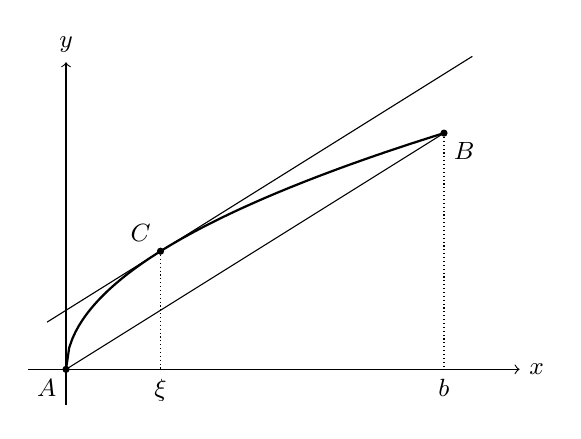
\begin{tikzpicture}[x=1.2cm,y=1.5cm,font=\small]
\draw[->] (-0.4,0)--(4.8,0) node[right] {$x$};
\draw[->] (0,-0.3)--(0,2.6) node[above] {$y$};
\draw[thick,domain=0:4,samples=120] plot (\x,{sqrt(\x)});
\draw (0,0)--(4,2);
\draw (-0.2,0.4)--(4.3,2.65);
\draw[densely dotted] (1,1)--(1,0) node[below] {$\xi$};
\draw[densely dotted] (4,2)--(4,0) node[below] {$b$};
\fill (0,0) circle (1.3pt);
\fill (4,2) circle (1.3pt);
\fill (1,1) circle (1.3pt);
\node[below left] at (0,0) {$A$};
\node[below right] at (4,2) {$B$};
\node[above left] at (1,1) {$C$};
\end{tikzpicture}
\end{center}

拉格朗日中值定理的两个条件也都不能去掉. 罗尔定理后举出的 $f_1$ 与 $f_2$ 分别不满足条件 (1) 与条件 (2), 它们的弦都是水平的, 导数却都不为零.

当 $a>b$ 时, 定理中的等式仍然成立. 这时在 $[b,a]$ 上应用定理, 得到 $f(a)-f(b)=f'(\xi)(a-b)$, 两边同时变号, 就是 $f(b)-f(a)=f'(\xi)(b-a)$, 其中 $\xi$ 介于 $a$ 与 $b$ 之间. 于是, 若 $f$ 在区间 $I$ 上连续, 在 $I$ 的内部可导, 则对 $I$ 中任意两点 $x$ 与 $x+\Delta x$ ($\Delta x\ne0$),
\[
f(x+\Delta x)-f(x)=f'(\xi)\Delta x\qquad(\xi\text{ 介于 }x\text{ 与 }x+\Delta x\text{ 之间}).
\]
把 $\xi$ 写成 $x+\theta\Delta x$, 即令 $\displaystyle\theta=\frac{\xi-x}{\Delta x}$. 由于 $\xi-x$ 与 $\Delta x$ 同号, 并且 $|\xi-x|<|\Delta x|$, 所以 $0<\theta<1$. 于是等式也可以写成 $f(x+\Delta x)-f(x)=f'(x+\theta\Delta x)\Delta x$, 这个等式称为\textbf{有限增量公式}. 2.5 节的 $\Delta y\approx f'(x)\Delta x$ 是近似式; 有限增量公式是准确的等式, 代价是 $\xi$ 的位置不确定, 只知道它的范围.
\begin{corollarysingle}
\textup{(1)} 若 $f$ 在区间 $I$ 上连续, 在 $I$ 的内部 $f'(x)=0$, 则 $f$ 在 $I$ 上是常数.

\textup{(2)} 若 $f,g$ 在区间 $I$ 上连续, 在 $I$ 的内部 $f'(x)=g'(x)$, 则在 $I$ 上 $f(x)=g(x)+C$, $C$ 是常数.
\end{corollarysingle}
\begin{cnproof}
(1) 在 $I$ 中任取两点 $x_1<x_2$. $f$ 在 $[x_1,x_2]$ 上连续; $(x_1,x_2)$ 含于 $I$ 的内部, 所以 $f$ 在 $(x_1,x_2)$ 内可导. 由拉格朗日中值定理, 存在 $\xi\in(x_1,x_2)$, 使 $f(x_2)-f(x_1)=f'(\xi)(x_2-x_1)$. $\xi$ 是 $I$ 的内点, $f'(\xi)=0$, 所以 $f(x_1)=f(x_2)$. $I$ 上任意两点的函数值都相等, $f$ 在 $I$ 上是常数. (2) 对 $f-g$ 应用 (1).
\end{cnproof}
\begin{example}\label{ex:c2-6-3}
\textnormal{(教材例6.3)} 证明: 当 $-1<x\le1$ 时,
\[
\arctan\sqrt{\frac{1-x}{1+x}}+\frac12\arcsin x=\frac\pi4.
\]
\end{example}
\par\indent\textbf{分析:} 要证一个函数在区间上恒等于常数, 由推论 (1), 只需证明它的导数恒为零, 再在一个方便的点算出这个常数. 在端点 $x=1$ 处 $\displaystyle\sqrt{\frac{1-x}{1+x}}$ 与 $\arcsin x$ 都不可导, 求导公式不能用, 所以只在 $(-1,1)$ 内求导, $x=1$ 处直接代入验证.
\begin{cnproof}
记左端为 $f(x)$. $x=1$ 时 $\displaystyle f(1)=\arctan0+\frac12\cdot\frac\pi2=\frac\pi4$. 设 $-1<x<1$, 令 $\displaystyle u=\sqrt{\frac{1-x}{1+x}}$, 则 $\displaystyle1+u^2=\frac2{1+x}$, 并且
\[
\begin{aligned}
u'&=\frac12\sqrt{\frac{1+x}{1-x}}\cdot\frac{-(1+x)-(1-x)}{(1+x)^2}=-\frac{\sqrt{1+x}}{\sqrt{1-x}\,(1+x)^2}\\
&=-\frac1{(1+x)\sqrt{1+x}\,\sqrt{1-x}}=-\frac1{(1+x)\sqrt{1-x^2}}.
\end{aligned}
\]
于是
\[
f'(x)=\frac{u'}{1+u^2}+\frac1{2\sqrt{1-x^2}}=-\frac1{(1+x)\sqrt{1-x^2}}\cdot\frac{1+x}2+\frac1{2\sqrt{1-x^2}}=0.
\]
由推论 (1), $f$ 在 $(-1,1)$ 上是常数, 代入 $x=0$ 得 $\displaystyle f(0)=\arctan1=\frac\pi4$. 连同 $x=1$ 的情形, 等式在 $(-1,1]$ 上成立.
\end{cnproof}
\begin{example}\label{ex:c2-6-4}
\textnormal{(教材例6.4)} 证明: 当 $x>0$ 时, $\displaystyle\frac x{1+x}<\ln(1+x)<x$.
\end{example}
\par\indent\textbf{分析:} 中间的 $\ln(1+x)=\ln(1+x)-\ln1$ 是函数 $\ln t$ 在区间 $[1,1+x]$ 上的增量. 由拉格朗日中值定理, 它等于 $\displaystyle\frac x\xi$, $1<\xi<1+x$. 把 $\displaystyle\frac x\xi$ 中的 $\xi$ 分别换成右端点 $1+x$ 与左端点 $1$, 恰好得到两端的 $\displaystyle\frac x{1+x}$ 与 $x$. 所以只需由 $\xi$ 的范围估计 $\displaystyle\frac1\xi$.
\begin{cnproof}
$\ln t$ 在 $[1,1+x]$ 上满足拉格朗日中值定理的条件, 所以存在 $\xi\in(1,1+x)$, 使
\[
\ln(1+x)=\ln(1+x)-\ln1=\frac x\xi.
\]
由 $1<\xi<1+x$ 及 $x>0$ 得 $\displaystyle\frac x{1+x}<\frac x\xi<x$.
\end{cnproof}
取 $\displaystyle x=\frac1n$, 得 $\displaystyle\frac1{n+1}<\ln\left(1+\frac1n\right)<\frac1n$ ($n\in\mathbb N^+$). 左边的不等式乘以 $n+1$, 右边的乘以 $n$, 再取指数, 就得到 $\displaystyle\left(1+\frac1n\right)^n<e<\left(1+\frac1n\right)^{n+1}$.
\begin{theorem}[柯西中值定理]\label{thm:c2-6-cauchy}
设 $f,g$ 满足: (1) 在闭区间 $[a,b]$ 上连续; (2) 在开区间 $(a,b)$ 内可导, 并且 $g'(x)\ne0$. 则存在 $\xi\in(a,b)$, 使
\[
\frac{f(b)-f(a)}{g(b)-g(a)}=\frac{f'(\xi)}{g'(\xi)}.
\]
\end{theorem}
\par\indent\textbf{分析:} 分别对 $f$ 和 $g$ 用拉格朗日中值定理再相除, 得到的是 $\displaystyle\frac{f'(\xi_1)}{g'(\xi_2)}$, 而 $\xi_1$ 与 $\xi_2$ 一般不同. 所以要像证明拉格朗日中值定理那样, 只对一个辅助函数用罗尔定理. 由罗尔定理和 $g'\ne0$ 可知 $g(b)\ne g(a)$, 所以可以记 $\displaystyle k=\frac{f(b)-f(a)}{g(b)-g(a)}$. 去分母后要证的是 $f'(\xi)-kg'(\xi)=0$. 左端是函数
\[
\varphi(x)=f(x)-f(a)-k\bigl(g(x)-g(a)\bigr)
\]
在 $\xi$ 处的导数, 其中的常数项 $-f(a)+kg(a)$ 不影响导数, 只是使 $\varphi(a)=0$; 由 $k$ 的取法, 又有 $\varphi(b)=f(b)-f(a)-k\bigl(g(b)-g(a)\bigr)=0$.
\begin{cnproof}
若 $g(b)=g(a)$, 由罗尔定理, $g'$ 在 $(a,b)$ 内有零点, 与条件矛盾, 所以 $g(b)\ne g(a)$. 记 $\displaystyle k=\frac{f(b)-f(a)}{g(b)-g(a)}$, 令
\[
\varphi(x)=f(x)-f(a)-k\bigl(g(x)-g(a)\bigr),
\]
则 $\varphi$ 在 $[a,b]$ 上连续, 在 $(a,b)$ 内可导, $\varphi(a)=\varphi(b)=0$. 由罗尔定理, 存在 $\xi\in(a,b)$, 使 $\varphi'(\xi)=f'(\xi)-kg'(\xi)=0$. 由 $g'(\xi)\ne0$ 得 $\displaystyle\frac{f'(\xi)}{g'(\xi)}=k$, 即所证等式.
\end{cnproof}
几何上, 把 $X=g(x)$, $Y=f(x)$ ($a\le x\le b$) 看作曲线的参数方程. 参数为 $a$ 与 $b$ 的两点连成一条弦, $k$ 是这条弦的斜率; 由 2.3 节参数方程的求导法则, $\displaystyle\frac{f'(\xi)}{g'(\xi)}$ 可以看作参数为 $\xi$ 的点处切线的斜率. 所以柯西中值定理是参数方程形式的拉格朗日中值定理. 取 $g(x)=x$, 它就是拉格朗日中值定理.
\begin{example}\label{ex:c2-6-5}
\textnormal{(教材例6.5)} 设 $f\in C[a,b]$, 在 $(a,b)$ 内可导, 并且 $f'(x)\ne0$. 证明存在 $\xi,\eta\in(a,b)$, 使
\[
\frac{f'(\xi)}{f'(\eta)}=\frac{(b-a)e^\xi}{e^b-e^a}.
\]
\end{example}
\par\indent\textbf{分析:} 等式中有两个中值点, 而每用一次中值定理只得到一个中值点, 所以先把 $\xi$ 与 $\eta$ 分到等式两边, 使每边只含一个:
\[
\frac{f'(\xi)}{e^\xi}=\frac{f'(\eta)(b-a)}{e^b-e^a}.
\]
左端是 $f$ 与 $e^x$ 的导数之比. 由柯西中值定理, 可以取 $\xi$ 使左端等于 $\displaystyle\frac{f(b)-f(a)}{e^b-e^a}$; 由拉格朗日中值定理, 可以取 $\eta$ 使右端分子中的 $f'(\eta)(b-a)$ 等于 $f(b)-f(a)$. 这样两端都化成同一个量 $\displaystyle\frac{f(b)-f(a)}{e^b-e^a}$.
\begin{cnproof}
对 $f$ 与 $g(x)=e^x$ 应用柯西中值定理 ($g'(x)=e^x\ne0$), 存在 $\xi\in(a,b)$, 使 $\displaystyle\frac{f(b)-f(a)}{e^b-e^a}=\frac{f'(\xi)}{e^\xi}$. 对 $f$ 应用拉格朗日中值定理, 存在 $\eta\in(a,b)$, 使 $f(b)-f(a)=f'(\eta)(b-a)$. 于是
\[
\frac{f'(\xi)}{e^\xi}=\frac{f'(\eta)(b-a)}{e^b-e^a},
\]
由 $f'(\eta)\ne0$, 两边除以 $f'(\eta)$ 再乘以 $e^\xi$ 即得结论.
\end{cnproof}
\begin{example}\label{ex:c2-h6-4}
\textnormal{(选自教材习题2.6第4题)} 设
\[
f(x)=\begin{cases}3-x^2,&0\le x\le1,\\\frac2x,&1<x\le2.\end{cases}
\]
$f$ 在 $[0,2]$ 上是否满足拉格朗日中值定理的条件? 在 $(0,2)$ 内满足 $f(2)-f(0)=2f'(\xi)$ 的 $\xi$ 有几个?
\end{example}
\begin{cnsolution}
在 $[0,1]$ 上 $f(x)=3-x^2$, 在 $(1,2]$ 上 $\displaystyle f(x)=\frac2x$, 两者在各自的区间上连续, 在区间内部可导, 只需检查分段点 $x=1$. $f(1)=2$, 右极限 $\displaystyle\lim_{x\to1^+}\frac2x=2$, 所以 $f$ 在 $1$ 连续. $x=1$ 时仍有 $f(x)=3-x^2$, 所以左导数为 $(3-x^2)'\big|_{x=1}=-2$; 右侧的差商为
\[
\frac{\frac2x-2}{x-1}=\frac{2-2x}{x(x-1)}=-\frac2x\to-2\quad(x\to1^+),
\]
左、右导数相等, $f'(1)=-2$. 所以条件满足.

$\xi$ 要满足 $\displaystyle f'(\xi)=\frac{f(2)-f(0)}2=\frac{1-3}2=-1$. 在 $(0,1]$ 上 $f'(\xi)=-2\xi=-1$ 得 $\displaystyle\xi=\frac12$; 在 $(1,2)$ 内 $\displaystyle f'(\xi)=-\frac2{\xi^2}=-1$ 得 $\xi=\sqrt2$. 所以这样的 $\xi$ 有两个.
\end{cnsolution}
\begin{example}\label{ex:c2-h6-6}
\textnormal{(选自教材习题2.6第6题(2)(6))} 用拉格朗日中值定理证明:

(2) 当 $\displaystyle0<\beta<\alpha<\frac\pi2$ 时, $\displaystyle\frac{\alpha-\beta}{\cos^2\beta}\le\tan\alpha-\tan\beta\le\frac{\alpha-\beta}{\cos^2\alpha}$;

(6) 当 $p>1$, $n\ge2$ 时, $\displaystyle\frac1{n^p}<\frac1{p-1}\left[\frac1{(n-1)^{p-1}}-\frac1{n^{p-1}}\right]$.
\end{example}
\par\indent\textbf{分析:} 两题中都有一个函数在两点的值之差. (2) 中是 $\tan t$ 在 $[\beta,\alpha]$ 上的增量. (6) 中方括号内是 $(n-1)^{1-p}-n^{1-p}$, 即 $t^{1-p}$ 在 $n-1$ 与 $n$ 处的值之差, 这个函数的导数中含 $t^{-p}$, 与左端的 $\displaystyle\frac1{n^p}$ 形式相同. 由拉格朗日中值定理, 这两个差都可以用 $f'(\xi)$ 和区间长度表示, 再由 $\xi$ 的范围和 $f'$ 的单调性估计 $f'(\xi)$.
\begin{cnproof}
(2) $\tan t$ 在 $[\beta,\alpha]$ 上连续、可导, 由拉格朗日中值定理, $\tan\alpha-\tan\beta=\sec^2\xi\cdot(\alpha-\beta)$, $\beta<\xi<\alpha$. 在 $\displaystyle\left(0,\frac\pi2\right)$ 内 $\cos t$ 是正的且严格减少, 所以 $\cos^2\alpha<\cos^2\xi<\cos^2\beta$, 即 $\displaystyle\frac1{\cos^2\beta}<\sec^2\xi<\frac1{\cos^2\alpha}$. 乘以 $\alpha-\beta>0$ 即得所证 (不等号是严格的).

(6) 令 $f(t)=t^{1-p}$, 它在 $[n-1,n]$ 上连续、可导 ($n-1\ge1$), $f'(t)=(1-p)t^{-p}$. 由拉格朗日中值定理,
\[
\frac1{(n-1)^{p-1}}-\frac1{n^{p-1}}=f(n-1)-f(n)=-f'(\xi)=\frac{p-1}{\xi^p},\qquad n-1<\xi<n.
\]
两边除以 $p-1>0$, 得 $\displaystyle\frac1{p-1}\left[\frac1{(n-1)^{p-1}}-\frac1{n^{p-1}}\right]=\frac1{\xi^p}$. 由 $0<\xi<n$ 及 $p>0$ 得 $\displaystyle\frac1{\xi^p}>\frac1{n^p}$, 即得所证.
\end{cnproof}
\begin{example}\label{ex:c2-h6-7}
\textnormal{(选自教材习题2.6第7题)} 设 $f\in C[a,b]$, 在 $(a,b)$ 内可导, $0<a<b$. 证明存在 $\xi\in(a,b)$, 使
\[
f(b)-f(a)=\xi f'(\xi)\ln\frac ba;
\]
并由此证明: 当 $x>0$ 时, $\displaystyle\lim_{n\to\infty}n\left(\sqrt[n]x-1\right)=\ln x$.
\end{example}
\par\indent\textbf{分析:} $\displaystyle\ln\frac ba=\ln b-\ln a$ 是 $\ln t$ 的增量, 所要证的等式可以写成
\[
\frac{f(b)-f(a)}{\ln b-\ln a}=\xi f'(\xi)=\frac{f'(\xi)}{\frac1\xi},
\]
右端是 $f'$ 与 $(\ln t)'$ 之比, 这是柯西中值定理的形式. 第二问中 $\sqrt[n]x-1$ 是 $t^{\frac1n}$ 在 $1$ 与 $x$ 之间的增量. 对 $f(t)=t^{\frac1n}$ 有 $\displaystyle\xi f'(\xi)=\frac1n\xi^{\frac1n}$, 由第一问, $\displaystyle\sqrt[n]x-1=\frac1n\xi^{\frac1n}\ln x$, 其中 $\xi$ 介于 $1$ 与 $x$ 之间, 并随 $n$ 变化. 当 $x>1$ 时 $1<\xi^{\frac1n}<x^{\frac1n}$, 可以用两边夹定理求 $\xi^{\frac1n}$ 的极限.
\begin{cnproof}
对 $f$ 与 $g(t)=\ln t$ 在 $[a,b]$ 上应用柯西中值定理 ($\displaystyle g'(t)=\frac1t\ne0$), 存在 $\xi\in(a,b)$, 使 $\displaystyle\frac{f(b)-f(a)}{\ln b-\ln a}=\xi f'(\xi)$, 即第一个等式.

设 $x>1$. $f(t)=t^{\frac1n}$ 在 $[1,x]$ 上连续, 在 $(1,x)$ 内可导, 对它在 $[1,x]$ 上应用第一个等式. 这时 $\displaystyle\xi f'(\xi)=\xi\cdot\frac1n\xi^{\frac1n-1}=\frac1n\xi^{\frac1n}$; 中值点随 $n$ 变化, 记为 $\xi_n$. 于是
\[
n\left(\sqrt[n]x-1\right)=\xi_n^{\frac1n}\ln x,\qquad1<\xi_n<x.
\]
由此 $1<\xi_n^{\frac1n}<x^{\frac1n}$, 而 $x^{\frac1n}\to1$ (1.4 节例\ref{ex:4-2}), 由两边夹定理 $\xi_n^{\frac1n}\to1$, 所以 $n\left(\sqrt[n]x-1\right)\to\ln x$. 当 $0<x<1$ 时, 在 $[x,1]$ 上应用第一个等式, 得 $\displaystyle1-\sqrt[n]x=\frac1n\xi_n^{\frac1n}\ln\frac1x$, 即 $n\left(\sqrt[n]x-1\right)=\xi_n^{\frac1n}\ln x$, $x<\xi_n<1$. 于是 $x^{\frac1n}<\xi_n^{\frac1n}<1$, 仍由两边夹定理得到结论. 当 $x=1$ 时两边都是 $0$.
\end{cnproof}
\begin{example}\label{ex:c2-h6-8}
\textnormal{(选自教材习题2.6第8题)} 设 $f$ 在有限区间 $(a,b)$ 内可导且无界. 证明 $f'$ 在 $(a,b)$ 内也无界; 并说明逆命题不成立.
\end{example}
\begin{cnproof}
只需证明逆否命题. 设 $|f'(x)|\le M$ ($x\in(a,b)$), 要证 $f$ 有界. 取定 $x_0\in(a,b)$. 对 $(a,b)$ 内任意 $x\ne x_0$, 以 $x_0$, $x$ 为端点的闭区间含于 $(a,b)$, $f$ 在这个区间上可导, 因而连续. 由拉格朗日中值定理, $f(x)-f(x_0)=f'(\xi)(x-x_0)$, 所以
\[
|f(x)|\le|f(x_0)|+M|x-x_0|\le|f(x_0)|+M(b-a),
\]
$f$ 有界. 逆命题不成立. 例如 $f(x)=\sqrt x$ 在 $(0,1)$ 内有界, 但 $\displaystyle f'(x)=\frac1{2\sqrt x}$ 在 $(0,1)$ 内无界.
\end{cnproof}
题目中区间有限的条件不能去掉. $f(x)=x$ 在 $(0,+\infty)$ 内无界, 而 $f'(x)=1$ 有界.
\begin{example}\label{ex:c2-h6-9}
\textnormal{(选自教材习题2.6第9题)} 设 $f\in C[a,b]$, 在 $(a,b)$ 内二阶可导, 连接点 $A(a,f(a))$ 与 $B(b,f(b))$ 的直线与曲线 $y=f(x)$ 还交于点 $C(c,f(c))$, $a<c<b$. 证明方程 $f''(x)=0$ 在 $(a,b)$ 内至少有一个实根.
\end{example}
\par\indent\textbf{分析:} 要得到 $f''$ 的零点, 可以对 $f'$ 用罗尔定理, 为此需要两个点使 $f'$ 的值相等. 三点共线说明弦 $AC$ 与弦 $CB$ 的斜率相等, 而由拉格朗日中值定理, 这两个斜率分别是 $f'$ 在 $(a,c)$ 与 $(c,b)$ 内某点的值.
\begin{cnproof}
$A,C,B$ 三点在同一条直线上, 所以弦 $AC$ 与弦 $CB$ 的斜率相等, 即 $\displaystyle\frac{f(c)-f(a)}{c-a}=\frac{f(b)-f(c)}{b-c}$. $f$ 在 $[a,b]$ 上连续, 在 $(a,b)$ 内二阶可导, 因而可导. 在 $[a,c]$ 与 $[c,b]$ 上分别应用拉格朗日中值定理, 存在 $\xi_1\in(a,c)$, $\xi_2\in(c,b)$, 使 $f'(\xi_1)$ 与 $f'(\xi_2)$ 分别等于这两个斜率, 因而 $f'(\xi_1)=f'(\xi_2)$. $f'$ 在 $(a,b)$ 内可导, 所以在 $[\xi_1,\xi_2]$ 上满足罗尔定理的条件, 存在 $\xi\in(\xi_1,\xi_2)\subseteq(a,b)$, 使 $f''(\xi)=0$.
\end{cnproof}
\begin{example}\label{ex:c2-h6-11}
\textnormal{(选自教材习题2.6第11题)} 设 $f,g$ 在 $\mathbb R$ 上可导. 证明: 在 $f$ 的任意两个零点之间, 方程 $f'(x)+g'(x)f(x)=0$ 至少有一个实根.
\end{example}
\par\indent\textbf{分析:} 设 $f(x_1)=f(x_2)=0$, $x_1<x_2$. 直接对 $f$ 用罗尔定理只能得到 $f'(\xi)=0$, 不含 $g$. 要找一个在 $x_1$, $x_2$ 处都为零的函数 $F$, 使 $F'$ 等于 $f'+g'f$ 乘一个不为零的因子. 为使 $F$ 在 $f$ 的零点处为零, 可以设 $F=fh$, 其中 $h$ 待定, 并且处处不为零. 这时 $\displaystyle F'=f'h+fh'=h\left(f'+\frac{h'}hf\right)$, 只需 $\displaystyle\frac{h'}h=g'$. 由 $(e^{g})'=g'e^{g}$, 取 $h=e^{g(x)}$ 即可.
\begin{cnproof}
设 $x_1<x_2$ 是 $f$ 的两个零点. 令 $F(x)=f(x)e^{g(x)}$, 则 $F$ 在 $[x_1,x_2]$ 上满足罗尔定理的条件, $F(x_1)=F(x_2)=0$. 所以存在 $\xi\in(x_1,x_2)$, 使
\[
F'(\xi)=e^{g(\xi)}\bigl[f'(\xi)+g'(\xi)f(\xi)\bigr]=0.
\]
由 $e^{g(\xi)}>0$ 得 $f'(\xi)+g'(\xi)f(\xi)=0$.
\end{cnproof}
\par\indent\textbf{方法小结:} 要证明存在一点 $\xi$ 使某个等式成立, 先把等式整理成 $H(\xi)=0$ 的形式. 再设法找到函数 $F$, 使 $F'$ 等于 $H$ 乘一个不为零的因子, 并且 $F$ 在两个端点的值相等, 然后对 $F$ 用罗尔定理. 观察 $H$ 是否像乘积的导数, 是找 $F$ 的常用办法. 等式中出现 $\displaystyle\frac{f(b)-f(a)}{b-a}$ 或 $\displaystyle\frac{f(b)-f(a)}{g(b)-g(a)}$ 时, 用拉格朗日或柯西中值定理; 有两个中值点时, 先把它们分到等式两边, 再分别用两个中值定理. 证明不等式时, 把其中一部分看作函数在两点的增量, 写成 $f'(\xi)$ 乘区间长度, 再由 $\xi$ 的范围估计 $f'(\xi)$. 要得到 $f''$ 的零点, 先在两个区间上分别对 $f$ 用拉格朗日中值定理, 得到 $f'$ 的值相等的两点, 再对 $f'$ 用罗尔定理.
\begin{example}\label{ex:c2-h6-13}
\textnormal{(选自教材习题2.6第13题)} 设 $f$ 在点 $a$ 的某个邻域 $U(a,r)$ 内连续, 在去心邻域 $\mathring U(a,r)$ 内可导, 并且 $\displaystyle\lim_{x\to a}f'(x)=l$. 证明 $f$ 在 $a$ 可导, 并且 $f'(a)=l$.
\end{example}
\par\indent\textbf{分析:} 要证差商 $\displaystyle\frac{f(x)-f(a)}{x-a}$ 趋于 $l$, 已知的却是导数 $f'(x)$ 的极限. 由拉格朗日中值定理, 差商等于 $f'(\xi)$, $\xi$ 介于 $a$ 与 $x$ 之间. $\xi$ 随 $x$ 而变, 但总有 $0<|\xi-a|<|x-a|$, 所以只要 $|x-a|$ 小于 $f'$ 的极限定义中的 $\delta$, 就有 $0<|\xi-a|<\delta$, 从而 $|f'(\xi)-l|<\varepsilon$. 这样直接用极限的定义就能证明, 不必把 $\xi$ 看作 $x$ 的函数再用复合函数的极限.
\begin{cnproof}
任给 $\varepsilon>0$, 由 $\displaystyle\lim_{x\to a}f'(x)=l$, 存在 $\delta\in(0,r)$, 使 $0<|t-a|<\delta$ 时 $|f'(t)-l|<\varepsilon$. 设 $0<|x-a|<\delta$. $f$ 在以 $a$ 与 $x$ 为端点的闭区间上连续, 在开区间内可导, 由拉格朗日中值定理, 存在介于 $a$ 与 $x$ 之间的 $\xi$, 使 $\displaystyle\frac{f(x)-f(a)}{x-a}=f'(\xi)$. 由 $0<|\xi-a|<|x-a|<\delta$ 得
\[
\left|\frac{f(x)-f(a)}{x-a}-l\right|=|f'(\xi)-l|<\varepsilon.
\]
所以 $f'(a)=l$.
\end{cnproof}
这个结论可以用来求分段函数在分段点的导数, 但要先验证 $f$ 在分段点连续. 例如 $f(x)=x$ ($x<0$), $f(x)=x+1$ ($x\ge0$), 当 $x\ne0$ 时 $f'(x)=1$, 但 $f$ 在 $0$ 不连续, 因而不可导.

把证明中的 $x$ 限制在 $a$ 的一侧, 同样可以得到单侧的结论. 若 $f$ 在 $[a,a+r)$ 上连续, 在 $(a,a+r)$ 内可导, 并且 $\displaystyle\lim_{x\to a^+}f'(x)=l$, 则 $f'_+(a)=l$; 左侧的情形相同. 由此可知, 若 $f$ 在区间上可导, 则 $f'$ 在区间内部没有第一类间断点. 事实上, 设 $a$ 是区间的内点, 并且 $f'$ 在 $a$ 处的左、右极限都存在. 由单侧的结论, 这两个极限分别等于 $f'_-(a)$ 与 $f'_+(a)$; 而 $f$ 在 $a$ 可导, 两者都等于 $f'(a)$, 所以 $f'$ 在 $a$ 连续. 导函数仍可能有间断点, 但只能是第二类的. 例如 2.2 节例\ref{ex:c2-h2-8} 中取 $n=2$, 得到 $\displaystyle h(x)=x^2\sin\frac1x$ ($x\ne0$), $h(0)=0$. 它处处可导, $h'(0)=0$; 而 $x\ne0$ 时 $\displaystyle h'(x)=2x\sin\frac1x-\cos\frac1x$. 其中第一项趋于 $0$, $\displaystyle\cos\frac1x$ 在 $0$ 的两侧都没有极限, 所以 $h'$ 在 $0$ 的两侧也都没有极限, $0$ 是 $h'$ 的第二类间断点.
\subsection{函数在区间上的单调性}
\begin{theorem}[单调性的判别]\label{thm:c2-6-mono}
设 $f$ 在区间 $I$ 上连续, 在 $I$ 的内部可导.

\textup{(1)} $f$ 在 $I$ 上单调增加 (减少) 的充分必要条件是: 在 $I$ 的内部 $f'(x)\ge0$ ($f'(x)\le0$).

\textup{(2)} $f$ 在 $I$ 上严格单调增加 (减少) 的充分必要条件是: 在 $I$ 的内部 $f'(x)\ge0$ ($f'(x)\le0$), 并且 $f'$ 在 $I$ 的任何长度为正的子区间上不恒为零.
\end{theorem}
\begin{cnproof}
只证增加的情形.

(1) 必要性. 设 $x$ 是 $I$ 的内点. 由 $f$ 单调增加, 不论 $\Delta x>0$ 还是 $\Delta x<0$, $f(x+\Delta x)-f(x)$ 都与 $\Delta x$ 同号或为零, 差商 $\displaystyle\frac{f(x+\Delta x)-f(x)}{\Delta x}\ge0$. 由保序性 (1.6 节定理1(3)), $f'(x)\ge0$. 充分性. 在 $I$ 中任取两点 $x_1<x_2$, 由拉格朗日中值定理, $f(x_2)-f(x_1)=f'(\xi)(x_2-x_1)$, 其中 $\xi$ 是 $I$ 的内点, $f'(\xi)\ge0$, 所以 $f(x_1)\le f(x_2)$.

(2) 必要性. 严格单调增加的函数是单调增加的, 由 (1), $f'\ge0$. 若 $f'$ 在某个子区间 $[c,d]$ ($c<d$) 上恒为零, 由拉格朗日中值定理的推论, $f$ 在 $[c,d]$ 上是常数, 与严格增加矛盾. 充分性. 由 (1), $f$ 单调增加. 若有 $x_1<x_2$ 使 $f(x_1)=f(x_2)$, 则对 $x_1<x<x_2$ 有 $f(x_1)\le f(x)\le f(x_2)=f(x_1)$, $f$ 在 $[x_1,x_2]$ 上是常数, $f'$ 在 $(x_1,x_2)$ 内恒为零, 与条件矛盾. 所以 $f$ 严格单调增加.
\end{cnproof}
特别地, 若在 $I$ 的内部 $f'(x)>0$, 则 $f$ 在 $I$ 上严格单调增加. 当 $f'\ge0$ 时, 导数为零的点只要不充满任何一个区间, 就不影响严格单调性; 导数为零的点只有有限个时, 这个条件显然满足. 例如 $x^3$ 在 $\mathbb R$ 上严格单调增加, 而 $(x^3)'\big|_{x=0}=0$.

定理\ref{thm:c2-6-mono} 要求 $I$ 是一个区间. $\displaystyle\frac1x$ 在 $(-\infty,0)$ 与 $(0,+\infty)$ 内的导数都是 $\displaystyle-\frac1{x^2}<0$, 它在这两个区间上分别严格单调减少, 但在定义域上不是单调减少的, 因为 $-1<1$, 而 $\displaystyle\frac1{-1}<\frac11$. $f$ 在 $I$ 的端点处连续的条件也不能去掉. 罗尔定理后举出的 $f_1$ 在 $(0,1)$ 内的导数为 $1$, 但 $\displaystyle f_1(1)=0<f_1\left(\frac12\right)$, 它在 $[0,1]$ 上不是单调增加的.

定理\ref{thm:c2-6-point} 由 $f'(x_0)>0$ 只能得到 $f$ 在点 $x_0$ 单调, 得不到 $f$ 在 $x_0$ 的某个邻域内单调. 例如 $\displaystyle f(x)=x+2x^2\sin\frac1x$ ($x\ne0$), $f(0)=0$. 在 $0$ 处差商为 $\displaystyle1+2x\sin\frac1x\to1$, $f'(0)=1>0$, 所以 $f$ 在 $0$ 严格单调增加. 而 $x\ne0$ 时 $\displaystyle f'(x)=1+4x\sin\frac1x-2\cos\frac1x$, 在 $\displaystyle x_k=\frac1{2k\pi}$ 处 $f'(x_k)=-1$. 这些点可以任意接近 $0$, 由定理\ref{thm:c2-6-mono} 的 (1), $f$ 在 $0$ 的任何邻域内都不是单调增加的. 图像上, $f$ 夹在两条抛物线 $y=x\pm2x^2$ 之间, 所以在原点附近, 左侧的点低于原点, 右侧的点高于原点. 但图像绕直线 $y=x$ 振荡, 振幅 $2x^2$ 虽然趋于零, 振荡却越来越快. 振荡部分 $\displaystyle2x^2\sin\frac1x$ 在每个 $x_k$ 处的斜率都是 $-2$, 下降得比直线 $y=x$ 上升得快, 所以在 $0$ 的任何邻域内都有下降的小段. 这个例子中 $f'$ 在 $0$ 不连续. 若 $f'$ 在 $x_0$ 连续且 $f'(x_0)>0$, 由保号性, $f'$ 在 $x_0$ 的某个邻域内为正, $f$ 在这个邻域内就严格单调增加.
\begin{example}\label{ex:c2-6-6}
\textnormal{(教材例6.6)} 证明: 当 $x\ge0$ 时, $\displaystyle\ln(1+x)\ge\frac{\arctan x}{1+x}$.
\end{example}
\par\indent\textbf{分析:} 比较两个函数的大小, 化为一个函数与零比较. 直接作差, 右端的商求导后较繁, 所以两边先乘以正数 $1+x$, 要证的是 $f(x)=(1+x)\ln(1+x)-\arctan x\ge0$. $f(0)=0$, 只需证明 $f$ 在 $[0,+\infty)$ 上单调增加, 也就是 $f'\ge0$.
\begin{cnproof}
令 $f(x)=(1+x)\ln(1+x)-\arctan x$, $x\ge0$. 则
\[
f'(x)=\ln(1+x)+1-\frac1{1+x^2}=\ln(1+x)+\frac{x^2}{1+x^2}>0\quad(x>0).
\]
由定理\ref{thm:c2-6-mono}, $f$ 在 $[0,+\infty)$ 上单调增加, $f(x)\ge f(0)=0$. 两边除以 $1+x>0$ 即得所证.
\end{cnproof}
若 $f$ 在区间 $J$ 上单调, 则称 $J$ 为 $f$ 的\textbf{单调区间}. 函数在整个定义区间上不一定单调. 求单调区间时, 用驻点和不可导点把定义区间分开; 若导数在每一部分内不变号, 由定理\ref{thm:c2-6-mono}, 函数在每一部分上单调. 当导数连续时, 这个条件总成立. 这是因为驻点都已取作分点, 每一部分内导数没有零点, 由零点定理, 它在这一部分内不变号.
\begin{example}\label{ex:c2-6-7}
\textnormal{(教材例6.7)} 求 $f(x)=x^3-6x^2+9x-2$ 的单调区间.
\end{example}
\begin{cnsolution}
$f'(x)=3x^2-12x+9=3(x-1)(x-3)$. 驻点 $x=1$, $x=3$ 把数轴分成三个区间, 在 $(-\infty,1)$ 与 $(3,+\infty)$ 内 $f'>0$, 在 $(1,3)$ 内 $f'<0$. $f$ 在分点处连续, 由定理\ref{thm:c2-6-mono}, 分点可以并入相邻的区间. 所以 $f$ 在 $(-\infty,1]$ 与 $[3,+\infty)$ 上严格单调增加, 在 $[1,3]$ 上严格单调减少.
\end{cnsolution}
\begin{example}\label{ex:c2-6-8}
\textnormal{(教材例6.8)} 设 $f$ 在 $[0,+\infty)$ 上二阶可导, $f''(x)<0$, $f(0)=0$. 证明: 对任意 $0<x_1<x_2$, 有 $f(x_1+x_2)<f(x_1)+f(x_2)$.
\end{example}
\par\indent\textbf{分析:} 已知的是 $f''$ 的符号, 它决定 $f'$ 的增减; 拉格朗日中值定理又能把 $f$ 的增量写成 $f'$ 的值乘区间长度. 所以设法把要证的不等式写成两个增量的比较. 由 $f(0)=0$, 它可以写成
\[
f(x_1+x_2)-f(x_2)<f(x_1)-f(0),
\]
两边分别是 $f$ 在区间 $[x_2,x_1+x_2]$ 与 $[0,x_1]$ 上的增量, 两个区间的长度都是 $x_1$. 由拉格朗日中值定理, 两边分别等于 $f'(\xi_2)x_1$ 与 $f'(\xi_1)x_1$. 由 $x_1<x_2$, 区间 $[x_2,x_1+x_2]$ 在 $[0,x_1]$ 的右边, 所以 $\xi_2>\xi_1$. 由 $f''<0$, $f'$ 严格减少, 因而 $f'(\xi_2)<f'(\xi_1)$.
\begin{cnproof}
$f$ 在 $[0,+\infty)$ 上可导, 因而连续. 由拉格朗日中值定理, 存在 $\xi_1\in(0,x_1)$, $\xi_2\in(x_2,x_1+x_2)$, 使
\[
f(x_1)-f(0)=f'(\xi_1)x_1,\qquad f(x_1+x_2)-f(x_2)=f'(\xi_2)x_1.
\]
$\xi_1<x_1<x_2<\xi_2$. $f'$ 在 $[0,+\infty)$ 上可导, 因而连续, 由 $f''<0$ 及定理\ref{thm:c2-6-mono}, $f'$ 在 $[0,+\infty)$ 上严格减少, $f'(\xi_2)<f'(\xi_1)$. 乘以 $x_1>0$ 并利用 $f(0)=0$, 得 $f(x_1+x_2)-f(x_2)<f(x_1)$.
\end{cnproof}
\begin{example}\label{ex:c2-h6-15}
\textnormal{(选自教材习题2.6第15题(2)(4))} 求下列函数的单调区间: (2) $y=\sqrt{2x-x^2}$; (4) $y=x+\lvert\sin2x\rvert$.
\end{example}
\begin{cnsolution}
(2) 定义域为 $[0,2]$. 当 $0<x<2$ 时 $\displaystyle y'=\frac{1-x}{\sqrt{2x-x^2}}$, 在 $(0,1)$ 内为正, 在 $(1,2)$ 内为负. 函数在 $[0,2]$ 上连续, 所以在 $[0,1]$ 上严格单调增加, 在 $[1,2]$ 上严格单调减少.

(4) $\lvert\sin2x\rvert$ 的周期为 $\displaystyle\frac\pi2$, 所以 $\displaystyle y\left(x+\frac\pi2\right)=y(x)+\frac\pi2$. 于是 $y$ 在每个区间 $\displaystyle\left[\frac{k\pi}2,\frac{(k+1)\pi}2\right]$ ($k\in\mathbb Z$) 上的图像由 $\displaystyle\left[0,\frac\pi2\right]$ 上的图像平移得到, 单调性相同. 在 $\displaystyle\left[0,\frac\pi2\right]$ 上 $\sin2x\ge0$, $y=x+\sin2x$; 在 $\displaystyle\left(0,\frac\pi2\right)$ 内 $y'=1+2\cos2x$. 当 $\displaystyle0<x<\frac\pi3$ 时 $\displaystyle\cos2x>-\frac12$, $y'>0$; 当 $\displaystyle\frac\pi3<x<\frac\pi2$ 时 $\displaystyle\cos2x<-\frac12$, $y'<0$. 所以 $y$ 在 $\displaystyle\left[\frac{k\pi}2,\frac{k\pi}2+\frac\pi3\right]$ 上严格增加, 在 $\displaystyle\left[\frac{k\pi}2+\frac\pi3,\frac{(k+1)\pi}2\right]$ 上严格减少 ($k\in\mathbb Z$). $y$ 在分点 $\displaystyle x=\frac{k\pi}2$ 处由减少变为增加. 由平移关系, $y$ 在这些点的左、右导数分别为 $1+2\cos\pi=-1$ 与 $1+2\cos0=3$, 所以这些分点是不可导点, 不是驻点.
\end{cnsolution}
\begin{example}\label{ex:c2-h6-16}
\textnormal{(选自教材习题2.6第16题(2)(3)(4)(5))} 证明下列不等式:
\[
\begin{gathered}
\text{(2)}\ \sin x+\tan x>2x,\quad\text{(3)}\ \tan x>x+\frac{x^3}3,\quad\text{(5)}\ \sin x>\frac2\pi x\qquad\left(0<x<\frac\pi2\right);\\
\text{(4)}\ 2^x>x^2\quad(x>4).
\end{gathered}
\]
\end{example}
\par\indent\textbf{分析:} (2)(3) 都化为 $F(x)>0$, 其中 $F(0)=0$, 只需证明 $F'>0$. (2) 中 $F'(x)=\cos x+\sec^2x-2$ 的符号不能一眼看出; 令 $c=\cos x\in(0,1)$, 则 $\displaystyle F'(x)=c+\frac1{c^2}-2=\frac{c^3-2c^2+1}{c^2}$, 分子在 $c=1$ 时为零, 可以分解出因子 $c-1$. (3) 中 $F'(x)=\sec^2x-1-x^2=\tan^2x-x^2$, 由 1.6 节例\ref{ex:6-5} 中的不等式 $x<\tan x$ ($\displaystyle0<x<\frac\pi2$) 即得 $F'>0$. (4) 中 $F(x)=2^x-x^2$, $F(4)=0$, 而 $F'(x)=2^x\ln2-2x$ 的符号仍看不出. 再求一次导数得 $F''(x)=2^x(\ln2)^2-2$, 它在 $x\ge4$ 时为正, 于是 $F'$ 严格增加, 只需 $F'(4)>0$. (5) 若直接作差, $\displaystyle\sin x-\frac2\pi x$ 的导数 $\displaystyle\cos x-\frac2\pi$ 在 $\displaystyle\left(0,\frac\pi2\right)$ 内由正变负, 要分两段讨论. 改写成 $\displaystyle\frac{\sin x}x>\frac2\pi$ 后, 左端是原点与点 $(x,\sin x)$ 连线的斜率, 右端是它在 $\displaystyle x=\frac\pi2$ 处的值, 所以只需证明 $\displaystyle\frac{\sin x}x$ 在 $\displaystyle\left(0,\frac\pi2\right]$ 上严格减少. 几何上, (5) 是说在 $\displaystyle\left(0,\frac\pi2\right)$ 内正弦曲线位于连接 $(0,0)$ 与 $\displaystyle\left(\frac\pi2,1\right)$ 的弦的上方.
\begin{cnproof}
(2) 令 $F(x)=\sin x+\tan x-2x$, $F(0)=0$. 记 $c=\cos x$, 则 $0<c<1$,
\[
F'(x)=c+\frac1{c^2}-2=\frac{c^3-2c^2+1}{c^2}=\frac{c^2(c-1)-(c-1)(c+1)}{c^2}=\frac{(c-1)(c^2-c-1)}{c^2}.
\]
$c-1<0$, $c^2-c-1=c(c-1)-1<0$, 所以 $F'(x)>0$. 由定理\ref{thm:c2-6-mono}, $F$ 在 $\displaystyle\left[0,\frac\pi2\right)$ 上严格增加, $F(x)>F(0)=0$.

(3) 令 $\displaystyle F(x)=\tan x-x-\frac{x^3}3$, 则 $F(0)=0$, 并且由 $\tan x>x>0$,
\[
F'(x)=\sec^2x-1-x^2=\tan^2x-x^2=(\tan x-x)(\tan x+x)>0,
\]
所以 $F$ 在 $\displaystyle\left[0,\frac\pi2\right)$ 上严格增加, $F(x)>F(0)=0$.

(4) 令 $F(x)=2^x-x^2$ ($x\ge4$), $F(4)=0$. 由 $e<4$ 得 $\ln4>1$, $\displaystyle\ln2>\frac12$. 当 $x\ge4$ 时 $\displaystyle F''(x)=2^x(\ln2)^2-2>16\cdot\frac14-2>0$, 由定理\ref{thm:c2-6-mono}, $F'$ 在 $[4,+\infty)$ 上严格增加; 又 $F'(4)=16\ln2-8=8(\ln4-1)>0$, 所以 $x>4$ 时 $F'(x)>0$, $F$ 在 $[4,+\infty)$ 上严格增加, $F(x)>F(4)=0$.

(5) 令 $\displaystyle G(x)=\frac{\sin x}x$, $\displaystyle0<x\le\frac\pi2$. $\displaystyle G'(x)=\frac{x\cos x-\sin x}{x^2}=\frac{\cos x\,(x-\tan x)}{x^2}<0$ ($\displaystyle0<x<\frac\pi2$), 所以 $G$ 在 $\displaystyle\left(0,\frac\pi2\right]$ 上严格减少, $\displaystyle G(x)>G\left(\frac\pi2\right)=\frac2\pi$, 即 $\displaystyle\sin x>\frac2\pi x$.
\end{cnproof}
(4) 也可以先取对数. $x>4$ 时不等式两边都是正数, 它等价于 $x\ln2>2\ln x$. 令 $H(x)=x\ln2-2\ln x$ ($x\ge4$), 则 $H(4)=4\ln2-2\ln4=0$; 当 $x>4$ 时 $\displaystyle H'(x)=\ln2-\frac2x>\ln2-\frac12>0$, 所以 $H$ 在 $[4,+\infty)$ 上严格增加, $H(x)>H(4)=0$. 这样只需求一次导数.
\par\indent\textbf{方法小结:} 用单调性证明不等式 $f(x)>g(x)$ ($x>a$) 时, 令 $F=f-g$, 检查 $F$ 在 $a$ 处连续并且 $F(a)\ge0$, 再证明 $F'>0$, 或 $F'\ge0$ 且不在任何区间上恒为零. 为了使导数简单, 可以先把不等式两边乘以正的因子, 或在两边都为正时取对数. 作差后的函数不单调时, 可以改写成商, 证明商单调, 再与端点处的值比较. $F'$ 的符号看不出时, 可以分解因式, 换元化为代数式, 或对 $F'$ 再求导. 求单调区间时, 用驻点和不可导点把定义区间分开, 逐段判断导数的符号.
\section{洛必达法则}
若当 $x\to a$ (或 $x\to\infty$) 时 $f(x)$ 与 $g(x)$ 都趋于零, 或者都是无穷大, 则称 $\displaystyle\lim\frac{f(x)}{g(x)}$ 为\textbf{不定式}, 分别简记为 $\displaystyle\frac00$ 型和 $\displaystyle\frac\infty\infty$ 型. 这时不能用商的极限法则, 而且仅由分子、分母的极限不能确定商的极限. 例如 $x\to0$ 时 $\displaystyle\frac{x^2}x\to0$, $\displaystyle\frac x{x^2}\to\infty$, $\displaystyle\frac{\sin x}x\to1$, 而 $\displaystyle\frac{x\sin\frac1x}x$ 没有极限.

第一章用恒等变形、重要极限和等价无穷小计算过许多不定式, 但那些办法要针对具体的式子去找. 导数提供了另一种办法. 若 $f(a)=g(a)=0$, $f,g$ 在 $a$ 可导, 并且 $g'(a)\ne0$, 则分子、分母同除以 $x-a$, 得
\[
\lim_{x\to a}\frac{f(x)}{g(x)}=\lim_{x\to a}\frac{\frac{f(x)-f(a)}{x-a}}{\frac{g(x)-g(a)}{x-a}}=\frac{f'(a)}{g'(a)}.
\]
但许多不定式不满足 $g'(a)\ne0$, 例如 $x\to0$ 时的 $\displaystyle\frac{x-\sin x}{x^3}$, 分子、分母在 $0$ 的导数都是零. 不过由 $\displaystyle1-\cos x\sim\frac{x^2}2$, 导数之比 $\displaystyle\frac{1-\cos x}{3x^2}$ 在 $x\to0$ 时仍有极限 $\displaystyle\frac16$. 本节用柯西中值定理证明, 可以把 $\displaystyle\frac{f'(a)}{g'(a)}$ 换成 $\displaystyle\lim_{x\to a}\frac{f'(x)}{g'(x)}$, 由此建立计算不定式的一般方法, 即洛必达 (L'Hospital, 1661--1704, 法国数学家) 法则.
\subsection{\texorpdfstring{$0/0$ 型与 $\infty/\infty$ 型不定式}{0/0 型与 ∞/∞ 型不定式}}
\begin{theorem}[$0/0$ 型的洛必达法则]\label{thm:c2-7-lh1}
设 $f,g$ 在 $\mathring U(a,r)$ 内可导, $g'(x)\ne0$, 并且

\textup{(1)} $\displaystyle\lim_{x\to a}f(x)=\lim_{x\to a}g(x)=0$;

\textup{(2)} $\displaystyle\lim_{x\to a}\frac{f'(x)}{g'(x)}=l$ ($l$ 可以是实数, 也可以是 $\infty$, $+\infty$ 或 $-\infty$).

则 $\displaystyle\lim_{x\to a}\frac{f(x)}{g(x)}=\lim_{x\to a}\frac{f'(x)}{g'(x)}=l$.
\end{theorem}
\par\indent\textbf{分析:} 定理不要求 $f,g$ 在 $a$ 可导, 条件 (2) 给出的是 $a$ 附近导数之比的极限. 要用上这个条件, 就要把函数值之比 $\displaystyle\frac{f(x)}{g(x)}$ 写成 $a$ 附近某一点处的导数之比. 柯西中值定理把两个函数增量之比写成导数之比. $f,g$ 在 $a$ 处的值与极限无关, 可以规定 $f(a)=g(a)=0$, 则 $f(x)=f(x)-f(a)$, $g(x)=g(x)-g(a)$ 都是增量. 由条件 (1), 这样规定后 $f,g$ 在 $a$ 连续, 柯西中值定理可以用在以 $a$ 与 $x$ 为端点的闭区间上:
\[
\frac{f(x)}{g(x)}=\frac{f(x)-f(a)}{g(x)-g(a)}=\frac{f'(\xi)}{g'(\xi)},\qquad\xi\text{ 介于 }a\text{ 与 }x\text{ 之间}.
\]
$\xi$ 随 $x$ 而变, 但总有 $0<|\xi-a|<|x-a|$. 任给 $\varepsilon>0$, 设 $\delta$ 是条件 (2) 的极限定义中与 $\varepsilon$ 对应的半径. 只要 $0<|x-a|<\delta$, 就有 $0<|\xi-a|<\delta$, 从而 $\displaystyle\left|\frac{f'(\xi)}{g'(\xi)}-l\right|<\varepsilon$. 对同一个 $x$, 柯西中值定理给出的 $\xi$ 可能不止一个, 不便把它看作 $x$ 的函数再用复合函数的极限, 所以这里直接用极限的定义; 2.6 节例\ref{ex:c2-h6-13} 中的中值点也是这样处理的.
\begin{cnproof}
补充定义 (或改变定义) $f(a)=g(a)=0$, 这不影响 $\displaystyle\frac{f(x)}{g(x)}$ 在 $x\to a$ 时的极限. $f,g$ 在 $\mathring U(a,r)$ 内可导, 因而连续; 由条件 (1), 它们在 $a$ 也连续. 设 $0<|x-a|<r$, 则 $f,g$ 在以 $a$ 与 $x$ 为端点的闭区间上满足柯西中值定理 (2.6 节定理\ref{thm:c2-6-cauchy}) 的条件. 这时 $g(x)=g(x)-g(a)\ne0$, 否则由罗尔定理, $g'$ 在 $a$ 与 $x$ 之间有零点. 由柯西中值定理, 存在介于 $a$ 与 $x$ 之间的 $\xi_x$, 使
\[
\frac{f(x)}{g(x)}=\frac{f(x)-f(a)}{g(x)-g(a)}=\frac{f'(\xi_x)}{g'(\xi_x)}.
\]
设 $l$ 是实数. 任给 $\varepsilon>0$, 由条件 (2), 存在 $\delta\in(0,r]$, 使 $0<|t-a|<\delta$ 时 $\displaystyle\left|\frac{f'(t)}{g'(t)}-l\right|<\varepsilon$. 当 $0<|x-a|<\delta$ 时, $0<|\xi_x-a|<|x-a|<\delta$, 所以
\[
\left|\frac{f(x)}{g(x)}-l\right|=\left|\frac{f'(\xi_x)}{g'(\xi_x)}-l\right|<\varepsilon.
\]
$l=\infty$ 时, 把 $\varepsilon$ 换成任意的 $M>0$, 把不等式换成 $\displaystyle\left|\frac{f'(t)}{g'(t)}\right|>M$, 就得到 $\displaystyle\left|\frac{f(x)}{g(x)}\right|>M$; $l=\pm\infty$ 的情形相同.
\end{cnproof}
对每个 $x$, 证明只用到 $a$ 与 $x$ 之间的点. 所以把条件中的 $\mathring U(a,r)$ 换成 $(a,a+r)$ 或 $(a-r,a)$, 同时把 $x\to a$ 相应地换成 $x\to a^+$ 或 $x\to a^-$, 定理同样成立.
\begin{theorem}[$x\to\infty$ 时的 $0/0$ 型]\label{thm:c2-7-lh2}
设 $f,g$ 在 $|x|>A$ ($A>0$) 时可导, $g'(x)\ne0$, $\displaystyle\lim_{x\to\infty}f(x)=\lim_{x\to\infty}g(x)=0$, 并且 $\displaystyle\lim_{x\to\infty}\frac{f'(x)}{g'(x)}=l$ ($l$ 可以是实数, 也可以是 $\infty$, $+\infty$ 或 $-\infty$). 则 $\displaystyle\lim_{x\to\infty}\frac{f(x)}{g(x)}=l$. 对 $x\to+\infty$ 与 $x\to-\infty$ 结论也成立 (条件中的 $|x|>A$ 相应地换成 $x>A$ 或 $x<-A$).
\end{theorem}
\begin{cnproof}
令 $\displaystyle t=\frac1x$, 把 $x\to\infty$ 化为 $t\to0$. 记 $\displaystyle F(t)=f\left(\frac1t\right)$, $\displaystyle G(t)=g\left(\frac1t\right)$, 它们在 $\displaystyle0<|t|<\frac1A$ 时有定义. $t\to0$ 时 $\displaystyle\frac1t\to\infty$, 由 1.6 节复合函数的极限, $F(t)\to0$, $G(t)\to0$. 由链式法则,
\[
\frac{F'(t)}{G'(t)}=\frac{f'\left(\frac1t\right)\cdot\left(-\frac1{t^2}\right)}{g'\left(\frac1t\right)\cdot\left(-\frac1{t^2}\right)}=\frac{f'\left(\frac1t\right)}{g'\left(\frac1t\right)}\to l\quad(t\to0),
\]
并且 $G'(t)\ne0$. 由定理\ref{thm:c2-7-lh1}, $\displaystyle\frac{F(t)}{G(t)}\to l$. 再令 $\displaystyle t=\frac1x$ 换回 ($x\to\infty$ 时 $t\to0$, 且 $t\ne0$), 得 $\displaystyle\lim_{x\to\infty}\frac{f(x)}{g(x)}=l$. 单侧的情形用 $t\to0^+$ 与 $t\to0^-$.
\end{cnproof}
这两个定理把求 $\displaystyle\frac fg$ 的极限转化为求 $\displaystyle\frac{f'}{g'}$ 的极限, 这种方法称为\textbf{洛必达法则}. 这里 $\displaystyle\frac{f'}{g'}$ 是分子、分母各自的导数之比, 不是商 $\displaystyle\frac fg$ 的导数. 若 $\displaystyle\frac{f'}{g'}$ 仍是 $\displaystyle\frac00$ 型, 并且 $f',g'$ 满足定理的条件, 可以继续使用. 用法则写出 $\displaystyle\lim\frac fg=\lim\frac{f'}{g'}$, 要求右端的极限存在 (或为 $\infty$), 而写下这个等式时, 右端往往还没有求出. 所以等式链要从右往左读. 求出最后一个极限以后, 才能依次得出前面的各个极限都等于它. 下面在使用法则的等号上方注明不定式的类型.
\begin{example}\label{ex:c2-7-1}
\textnormal{(教材例7.1)} 求 $\displaystyle\lim_{x\to1}\frac{\sin\pi x}{\ln x}$.
\end{example}
\begin{cnsolution}
$x\to1$ 时分子、分母都趋于零, 是 $\displaystyle\frac00$ 型; 在 $1$ 附近 $\displaystyle(\ln x)'=\frac1x\ne0$. 所以
\[
\lim_{x\to1}\frac{\sin\pi x}{\ln x}\overset{0/0}{=}\lim_{x\to1}\frac{\pi\cos\pi x}{\frac1x}=\pi\cos\pi=-\pi.
\]
\end{cnsolution}
\begin{example}\label{ex:c2-7-2}
\textnormal{(教材例7.2)} 求 $\displaystyle\lim_{x\to+\infty}\frac{\frac\pi2-\arctan x}{\sin\frac1x}$.
\end{example}
\begin{cnsolution}
$x\to+\infty$ 时 $\displaystyle\arctan x\to\frac\pi2$, $\displaystyle\sin\frac1x\to0$, 是 $\displaystyle\frac00$ 型. 当 $\displaystyle x>\frac2\pi$ 时 $\displaystyle0<\frac1x<\frac\pi2$, 分母的导数 $\displaystyle-\frac1{x^2}\cos\frac1x\ne0$. 由定理\ref{thm:c2-7-lh2},
\[
\lim_{x\to+\infty}\frac{\frac\pi2-\arctan x}{\sin\frac1x}\overset{0/0}{=}\lim_{x\to+\infty}\frac{-\frac1{1+x^2}}{-\frac1{x^2}\cos\frac1x}=\lim_{x\to+\infty}\frac{x^2}{1+x^2}\cdot\frac1{\cos\frac1x}=1.
\]
\end{cnsolution}
\begin{example}\label{ex:c2-7-3}
\textnormal{(教材例7.3)} 求 $\displaystyle\lim_{x\to0}\frac{e^x-e^{-x}-2x}{x-\sin x}$.
\end{example}
\begin{cnsolution}
$\displaystyle\frac00$ 型. 第一次求导后, 分子 $e^x+e^{-x}-2$ 与分母 $1-\cos x$ 仍都趋于零; 第二次求导后, 分子 $e^x-e^{-x}$ 与分母 $\sin x$ 也都趋于零. 在 $0$ 的去心邻域 $\displaystyle0<|x|<\frac\pi2$ 内, 依次求导得到的分母 $1-\cos x$, $\sin x$, $\cos x$ 都不为零, 所以可以连续用三次法则:
\[
\lim_{x\to0}\frac{e^x-e^{-x}-2x}{x-\sin x}\overset{0/0}{=}\lim_{x\to0}\frac{e^x+e^{-x}-2}{1-\cos x}\overset{0/0}{=}\lim_{x\to0}\frac{e^x-e^{-x}}{\sin x}\overset{0/0}{=}\lim_{x\to0}\frac{e^x+e^{-x}}{\cos x}=2.
\]
\end{cnsolution}
对 $\displaystyle\frac\infty\infty$ 型有相应的法则.
\begin{theorem}[$\infty/\infty$ 型的洛必达法则]\label{thm:c2-7-lh3}
设 $f,g$ 在 $\mathring U(a,r)$ 内可导, $g'(x)\ne0$, $\displaystyle\lim_{x\to a}f(x)=\lim_{x\to a}g(x)=\infty$, 并且 $\displaystyle\lim_{x\to a}\frac{f'(x)}{g'(x)}=l$ ($l$ 可以是实数, 也可以是 $\infty$, $+\infty$ 或 $-\infty$). 则 $\displaystyle\lim_{x\to a}\frac{f(x)}{g(x)}=l$. 对单侧极限以及 $x\to\infty$ ($x\to\pm\infty$) 结论也成立 (条件中的 $\mathring U(a,r)$ 换成相应的范围).
\end{theorem}
\par\indent\textbf{分析:} 以 $x\to a^+$, $l$ 为实数为例. 这时 $g$ 在 $a$ 附近无界, 不论怎样规定 $g(a)$, 它在 $a$ 都不连续, 不能在以 $a$ 为端点的区间上用柯西中值定理. 改为在 $a$ 的右侧取一个固定点 $y$, 对 $a<x<y$, 在 $[x,y]$ 上用柯西中值定理:
\[
Q=\frac{f(x)-f(y)}{g(x)-g(y)}=\frac{f'(\xi)}{g'(\xi)},\qquad x<\xi<y.
\]
$\xi$ 总在 $(a,y)$ 内, 所以只要 $y$ 离 $a$ 足够近, 不论 $x$ 取 $(a,y)$ 中哪一点, $Q$ 都接近 $l$. 剩下的问题是从 $Q$ 回到 $\displaystyle\frac{f(x)}{g(x)}$. 把 $f(x)=f(y)+Q\bigl(g(x)-g(y)\bigr)$ 两边除以 $g(x)$, 得
\[
\frac{f(x)}{g(x)}=\frac{f(y)}{g(x)}+\left(1-\frac{g(y)}{g(x)}\right)Q.
\]
$y$ 取定以后, $x\to a^+$ 时 $|g(x)|\to+\infty$, 右端第一项趋于零, 括号内趋于 $1$, 而 $Q$ 接近 $l$, 所以 $\displaystyle\frac{f(x)}{g(x)}$ 也接近 $l$. 但 $y$ 固定时, 只知道 $\xi$ 在 $(x,y)$ 内, 它不一定趋于 $a$, 由此推不出 $Q\to l$, 只能利用取 $y$ 时得到的 $|Q-l|$ 的上界. 为此把 $Q=l+(Q-l)$ 代入, 两边减去 $l$, 得
\[
\begin{aligned}
\frac{f(x)}{g(x)}-l&=\frac{f(y)}{g(x)}+\left(1-\frac{g(y)}{g(x)}\right)l-l+\left(1-\frac{g(y)}{g(x)}\right)(Q-l)\\
&=\frac{f(y)-lg(y)}{g(x)}+\left(1-\frac{g(y)}{g(x)}\right)(Q-l).
\end{aligned}
\]
先由 $\varepsilon$ 取定 $y$, 使对 $(a,y)$ 中的每个 $x$ 都有 $\displaystyle|Q-l|<\frac\varepsilon2$. 再由 $|g(x)|\to+\infty$, 让 $x$ 离 $a$ 足够近, 使右端第一项的绝对值小于 $\displaystyle\frac\varepsilon4$, 并使 $\displaystyle\left|\frac{g(y)}{g(x)}\right|<\frac12$; 这时括号的绝对值小于 $\displaystyle\frac32$, 第二项的绝对值小于 $\displaystyle\frac{3\varepsilon}4$. $x$ 离 $a$ 多近才够, 要由 $f(y)$ 与 $g(y)$ 决定, 所以 $y$ 必须先取定.
\begin{cnproof}
只证 $x\to a^+$, $l$ 为实数的情形. 任给 $\varepsilon>0$. 由条件, 存在 $\delta_1\in(0,r)$, 使 $a<t<a+\delta_1$ 时 $\displaystyle\left|\frac{f'(t)}{g'(t)}-l\right|<\frac\varepsilon2$. 取定 $y=a+\delta_1$. 由 $g(x)\to\infty$, 存在 $\delta_2\in(0,\delta_1)$, 使 $a<x<a+\delta_2$ 时
\[
|g(x)|>\max\left\{2|g(y)|,\ \frac{4|f(y)-lg(y)|}\varepsilon\right\}
\]
(右端不小于零, 所以 $g(x)\ne0$). 设 $a<x<a+\delta_2$. 在 $[x,y]$ 上应用柯西中值定理 (这时 $g(x)\ne g(y)$), 存在 $\xi\in(x,y)$, 使 $\displaystyle Q=\frac{f(x)-f(y)}{g(x)-g(y)}=\frac{f'(\xi)}{g'(\xi)}$. 因为 $\xi\in(x,y)\subseteq(a,a+\delta_1)$, 所以 $\displaystyle|Q-l|<\frac\varepsilon2$. 由 $f(x)=f(y)+Q\bigl(g(x)-g(y)\bigr)$,
\[
\frac{f(x)}{g(x)}-l=\frac{f(y)}{g(x)}+\left(1-\frac{g(y)}{g(x)}\right)Q-l=\frac{f(y)-lg(y)}{g(x)}+\left(1-\frac{g(y)}{g(x)}\right)(Q-l),
\]
其中第二个等号是把 $Q$ 写成 $l+(Q-l)$ 后整理得到的. 由 $\delta_2$ 的取法, $\displaystyle\frac{|f(y)-lg(y)|}{|g(x)|}<\frac\varepsilon4$, $\displaystyle\left|\frac{g(y)}{g(x)}\right|<\frac12$, 所以
\[
\left|\frac{f(x)}{g(x)}-l\right|\le\frac{|f(y)-lg(y)|}{|g(x)|}+\left(1+\left|\frac{g(y)}{g(x)}\right|\right)|Q-l|<\frac\varepsilon4+\frac32\cdot\frac\varepsilon2=\varepsilon.
\]
\end{cnproof}
$l$ 为 $\infty$ 时, 把 $f(x)=f(y)+Q\bigl(g(x)-g(y)\bigr)$ 两边除以 $g(x)$, 得
\[
\frac{f(x)}{g(x)}=\frac{f(y)}{g(x)}+\left(1-\frac{g(y)}{g(x)}\right)Q.
\]
任给 $M>0$, 取 $\delta_1\in(0,r)$, 使 $a<t<a+\delta_1$ 时 $\displaystyle\left|\frac{f'(t)}{g'(t)}\right|>2M+2$, 并取定 $y=a+\delta_1$. 对 $(a,y)$ 中的每个 $x$, 中值点 $\xi\in(x,y)\subseteq(a,a+\delta_1)$, 所以 $|Q|>2M+2$. 再取 $\delta_2\in(0,\delta_1)$, 使 $a<x<a+\delta_2$ 时 $\displaystyle\left|\frac{g(y)}{g(x)}\right|<\frac12$, $\displaystyle\left|\frac{f(y)}{g(x)}\right|<1$. 这时
\[
\left|\frac{f(x)}{g(x)}\right|\ge\left(1-\left|\frac{g(y)}{g(x)}\right|\right)|Q|-\left|\frac{f(y)}{g(x)}\right|>\frac12(2M+2)-1=M.
\]
$l=+\infty$ 时, 把 $\delta_1$ 的取法中的不等式换成 $\displaystyle\frac{f'(t)}{g'(t)}>2M+2$, 则 $Q>2M+2$, 再由 $\displaystyle1-\frac{g(y)}{g(x)}>\frac12$ 及 $\displaystyle\frac{f(y)}{g(x)}>-1$ 得 $\displaystyle\frac{f(x)}{g(x)}>\frac12(2M+2)-1=M$; $l=-\infty$ 时对 $-f$ 用这个结论. $x\to a^-$ 的情形相同, 双侧的极限由两个单侧极限得到; $x\to\infty$ 的情形仿照定理\ref{thm:c2-7-lh2} 的证明, 令 $\displaystyle t=\frac1x$.
\begin{example}\label{ex:c2-7-4}
\textnormal{(教材例7.4)} 设 $\mu>0$, 求 $\displaystyle\lim_{x\to+\infty}\frac{\ln x}{x^\mu}$.
\end{example}
\begin{cnsolution}
$\displaystyle\frac\infty\infty$ 型, $(x^\mu)'=\mu x^{\mu-1}\ne0$ ($x>0$). 所以
\[
\lim_{x\to+\infty}\frac{\ln x}{x^\mu}\overset{\infty/\infty}{=}\lim_{x\to+\infty}\frac{\frac1x}{\mu x^{\mu-1}}=\lim_{x\to+\infty}\frac1{\mu x^\mu}=0.
\]
\end{cnsolution}
\begin{example}\label{ex:c2-7-5}
\textnormal{(教材例7.5)} 设 $a>1$, $\mu>0$, 求 $\displaystyle\lim_{x\to+\infty}\frac{x^\mu}{a^x}$.
\end{example}
\par\indent\textbf{分析:} $\displaystyle\frac\infty\infty$ 型. 每用一次法则, 分子中 $x$ 的指数减少 $1$ 并多出一个常数因子, 分母仍是 $a^x$ 乘一个常数. 指数还为正时分子仍趋于无穷, 可以继续用; 指数降到不大于零时, 分子在 $x\ge1$ 时有界, 而分母趋于无穷, 极限为零. 所以用法则的次数取为使 $\mu-k\le0$ 的最小正整数 $k$, 即 $k-1<\mu\le k$.
\begin{cnsolution}
取正整数 $k$ 使 $k-1<\mu\le k$. 对 $1\le j\le k-1$, 用 $j$ 次法则后得到
\[
\frac{\mu(\mu-1)\cdots(\mu-j+1)x^{\mu-j}}{a^x(\ln a)^j},
\]
其中 $\mu-j>0$, 仍是 $\displaystyle\frac\infty\infty$ 型, 可以继续用. 用 $k$ 次后得到 $\displaystyle\frac{\mu(\mu-1)\cdots(\mu-k+1)x^{\mu-k}}{a^x(\ln a)^k}$, 其中 $\mu-k\le0$, $x\ge1$ 时 $0<x^{\mu-k}\le1$, 而 $a^x\to+\infty$, 所以它趋于 $0$. 从最后一步往前依次用法则, 得
\[
\lim_{x\to+\infty}\frac{x^\mu}{a^x}=0.
\]
\end{cnsolution}
例\ref{ex:c2-7-4}, \ref{ex:c2-7-5} 说明, $x\to+\infty$ 时 $\ln x$, $x^\mu$, $a^x$ ($\mu>0$, $a>1$) 都是正无穷大, 但对数函数比任何正次幂增长得慢, 幂函数又比指数函数增长得慢; 按 1.7 节的说法, $\ln x$ 是比 $x^\mu$ 低阶的无穷大, $x^\mu$ 是比 $a^x$ 低阶的无穷大.
\begin{example}\label{ex:c2-7-6}
\textnormal{(教材例7.6)} 设
\[
f(x)=\begin{cases}e^{-\frac1{x^2}},&x\ne0,\\0,&x=0.\end{cases}
\]
证明 $f$ 在 $x=0$ 处有各阶导数, 并且 $f^{(n)}(0)=0$ ($n\in\mathbb N^+$).
\end{example}
\par\indent\textbf{分析:} 按定义, $\displaystyle f^{(n)}(0)=\lim_{x\to0}\frac{f^{(n-1)}(x)-f^{(n-1)}(0)}x$, 所以需要 $x\ne0$ 时 $f^{(n-1)}(x)$ 的表达式. 求前两阶:
\[
f'(x)=\frac2{x^3}e^{-\frac1{x^2}},\qquad f''(x)=\left(-\frac6{x^4}+\frac4{x^6}\right)e^{-\frac1{x^2}}\quad(x\ne0),
\]
都是 $\displaystyle\frac1x$ 的多项式乘以 $e^{-\frac1{x^2}}$. 对 $n$ 归纳. 若已知 $f^{(n-1)}(0)=0$, 则差商就是 $\displaystyle\frac{f^{(n-1)}(x)}x$, 它是若干项 $\displaystyle\frac c{x^m}e^{-\frac1{x^2}}$ 之和. 令 $\displaystyle t=\frac1{x^2}$, 每一项的绝对值是 $\displaystyle|c|\frac{t^{\frac m2}}{e^t}$, 由例\ref{ex:c2-7-5}, $t\to+\infty$ 时它趋于零.
\begin{cnproof}
(1) 对每个 $k\in\mathbb N$, 存在多项式 $P_k$, 使 $x\ne0$ 时 $\displaystyle f^{(k)}(x)=P_k\left(\frac1x\right)e^{-\frac1{x^2}}$. $k=0$ 时 $P_0=1$. 若对 $k$ 成立, 则 $x\ne0$ 时
\[
f^{(k+1)}(x)=\left[P_k'\left(\frac1x\right)\cdot\left(-\frac1{x^2}\right)+P_k\left(\frac1x\right)\cdot\frac2{x^3}\right]e^{-\frac1{x^2}},
\]
令 $P_{k+1}(u)=-u^2P_k'(u)+2u^3P_k(u)$, 它是多项式, 结论对 $k+1$ 成立.

(2) 对任意多项式 $P$, $\displaystyle\lim_{x\to0}P\left(\frac1x\right)e^{-\frac1{x^2}}=0$. 只需对每个单项 $u^m$ 证明. 令 $\displaystyle t=\frac1{x^2}$, 则 $x\to0$ 时 $t\to+\infty$, 并且
\[
\left|\frac1{x^m}e^{-\frac1{x^2}}\right|=\frac{t^{\frac m2}}{e^t},
\]
$m\ge1$ 时由例\ref{ex:c2-7-5} ($a=e$, $\displaystyle\mu=\frac m2$) 趋于零, $m=0$ 时 $e^{-t}\to0$.

(3) 对 $n$ 归纳. $\displaystyle f'(0)=\lim_{x\to0}\frac{e^{-\frac1{x^2}}}x=\lim_{x\to0}\frac1xe^{-\frac1{x^2}}=0$ (由 (2), $P(u)=u$). 若 $f^{(k)}(0)=0$, 则由 (1) 写出差商, 再对多项式 $uP_k(u)$ 用 (2), 得
\[
f^{(k+1)}(0)=\lim_{x\to0}\frac{f^{(k)}(x)-0}x=\lim_{x\to0}\frac1xP_k\left(\frac1x\right)e^{-\frac1{x^2}}=0.
\]
所以对一切 $n\in\mathbb N^+$, $f^{(n)}(0)=0$.
\end{cnproof}
$f$ 与恒为零的函数在 $0$ 处的各阶导数完全相同, 但 $x\ne0$ 时 $f(x)>0$. 可见只知道函数在一点处的各阶导数, 还不能确定函数在这一点附近的值.

使用洛必达法则时, 每一步都要检查是否仍是 $\displaystyle\frac00$ 或 $\displaystyle\frac\infty\infty$ 型, 不是这两种类型就不能再用. 例如
\[
\lim_{x\to0}\frac{e^x-1}{x^2+x}\overset{0/0}{=}\lim_{x\to0}\frac{e^x}{2x+1}=1,
\]
其中第二个极限的分子、分母都趋于 $1$, 不满足定理\ref{thm:c2-7-lh1} 的条件 (1); 若对它再用一次法则, 会得到错误的结果 $\displaystyle\lim_{x\to0}\frac{e^x}2=\frac12$.

洛必达法则可以与等价无穷小替换、换元等方法结合使用. 极限不为零的因子应当先求出极限, 分离出去, 使剩下的不定式求导简单.
\begin{example}\label{ex:c2-7-7}
\textnormal{(教材例7.7)} 求 $\displaystyle\lim_{x\to0}\frac{(e^x-1-x)^2}{x\sin^3x}$.
\end{example}
\begin{cnsolution}
$\displaystyle\frac00$ 型. 直接求导, 分子、分母的导数都很繁. 先把分母中的 $\sin^3x$ 换成等价无穷小 $x^3$, 原式化为 $\displaystyle\frac{(e^x-1-x)^2}{x^4}=\left(\frac{e^x-1-x}{x^2}\right)^2$. 由 $t^2$ 的连续性, 只需求括号内的极限, 它是 $\displaystyle\frac00$ 型:
\[
\lim_{x\to0}\frac{(e^x-1-x)^2}{x\sin^3x}=\lim_{x\to0}\frac{(e^x-1-x)^2}{x^4}=\left[\lim_{x\to0}\frac{e^x-1-x}{x^2}\right]^2\overset{0/0}{=}\left[\lim_{x\to0}\frac{e^x-1}{2x}\right]^2=\left(\frac12\right)^2=\frac14,
\]
其中 $\displaystyle\lim_{x\to0}\frac{e^x-1}{2x}=\frac12$ 由 $e^x-1\sim x$ 得到.
\end{cnsolution}
\begin{example}\label{ex:c2-7-8}
\textnormal{(教材例7.8)} 求 $\displaystyle\lim_{x\to a}\frac{e^{\cos x}\ln|x-a|}{\ln|e^x-e^a|}$.
\end{example}
\begin{cnsolution}
因子 $e^{\cos x}$ 的极限 $e^{\cos a}\ne0$, 先分离出去. 剩下的 $\displaystyle\frac{\ln|x-a|}{\ln|e^x-e^a|}$ 中, $x\to a$ 时分子、分母都趋于 $-\infty$, 是 $\displaystyle\frac\infty\infty$ 型. 由 $\displaystyle(\ln|u|)'=\frac{u'}u$, 分子、分母的导数分别是 $\displaystyle\frac1{x-a}$ 与 $\displaystyle\frac{e^x}{e^x-e^a}$, 后者在 $x\ne a$ 处不为零. 导数之比中的因子 $\displaystyle\frac{e^x-e^a}{x-a}$ 正是 $e^x$ 在 $a$ 处的差商, 它趋于 $e^a$:
\[
\lim_{x\to a}\frac{e^{\cos x}\ln|x-a|}{\ln|e^x-e^a|}=e^{\cos a}\lim_{x\to a}\frac{\ln|x-a|}{\ln|e^x-e^a|}\overset{\infty/\infty}{=}e^{\cos a}\lim_{x\to a}\left(\frac{e^x-e^a}{x-a}\cdot\frac1{e^x}\right)=e^{\cos a}\cdot e^a\cdot\frac1{e^a}=e^{\cos a}.
\]
\end{cnsolution}
洛必达法则给出的只是充分条件. $\displaystyle\frac{f'}{g'}$ 的极限存在 (或为 $\infty$) 时, $\displaystyle\frac fg$ 有相同的极限; 反过来, $\displaystyle\frac fg$ 的极限存在时, $\displaystyle\frac{f'}{g'}$ 的极限不一定存在. 所以 $\displaystyle\frac{f'}{g'}$ 的极限不存在而且不是 $\infty$ 时, 只能说法则不适用, 不能由此断定 $\displaystyle\frac fg$ 的极限不存在. 例如 $\displaystyle\lim_{x\to0}\frac{x^2\sin\frac1x}{\sin x}$ 是 $\displaystyle\frac00$ 型, 而
\[
\frac{\left(x^2\sin\frac1x\right)'}{(\sin x)'}=\frac{2x\sin\frac1x-\cos\frac1x}{\cos x},
\]
与 2.2 节例\ref{ex:c2-h2-8} 一样, 取 $\displaystyle x_k=\frac1{2k\pi}$, $\displaystyle y_k=\frac1{(2k+1)\pi}$ ($k\in\mathbb N^+$), 在这两列点处 $\displaystyle\sin\frac1x=0$, $\displaystyle\cos\frac1x$ 分别等于 $1$ 与 $-1$, 所以导数之比分别等于 $\displaystyle-\frac1{\cos x_k}$ 与 $\displaystyle\frac1{\cos y_k}$, 趋于 $-1$ 与 $1$. 由海涅定理, 导数之比没有极限, 也不是 $\infty$. 但原极限存在:
\[
\lim_{x\to0}\frac{x^2\sin\frac1x}{\sin x}=\lim_{x\to0}\frac x{\sin x}\cdot\lim_{x\to0}x\sin\frac1x=1\cdot0=0.
\]
\begin{example}\label{ex:c2-h7-2}
\textnormal{(选自教材习题2.7第2题)} 验证极限 $\displaystyle\lim_{x\to\infty}\frac{x-\sin x}{x+\sin x}$ 存在, 但不能用洛必达法则计算.
\end{example}
\begin{cnsolution}
分子、分母同除以 $x$, 由 $\displaystyle\left|\frac{\sin x}x\right|\le\frac1{|x|}\to0$,
\[
\lim_{x\to\infty}\frac{x-\sin x}{x+\sin x}=\lim_{x\to\infty}\frac{1-\frac{\sin x}x}{1+\frac{\sin x}x}=1.
\]
这是 $\displaystyle\frac\infty\infty$ 型, 但分母的导数 $1+\cos x$ 在 $x=(2k+1)\pi$ ($k\in\mathbb Z$) 处为零, 这些点的绝对值可以任意大, 所以不论 $A$ 多大, 都不满足 $|x|>A$ 时 $g'(x)\ne0$ 的条件; 导数之比 $\displaystyle\frac{1-\cos x}{1+\cos x}$ 在 $x=2k\pi$ 处为 $0$, 在 $\displaystyle x=2k\pi+\frac\pi2$ 处为 $1$, 也没有极限. 所以不能用洛必达法则.
\end{cnsolution}
\subsection{其他类型的不定式}
除 $\displaystyle\frac00$ 与 $\displaystyle\frac\infty\infty$ 型外, 还有 $0\cdot\infty$, $\infty-\infty$, $0^0$, $1^\infty$, $\infty^0$ 五种类型的不定式. 它们与 $\displaystyle\frac00$ 型一样, 仅由各部分的极限不能确定整个式子的极限, 例如 1.6 节的第二个重要极限是 $1^\infty$ 型, 极限是 $e$ 而不是 $1$. 这五种不定式都可以化为 $\displaystyle\frac00$ 或 $\displaystyle\frac\infty\infty$ 型.

(1) $0\cdot\infty$ 型: $f\to0$, $g\to\infty$. 写成 $\displaystyle fg=\frac f{\frac1g}$ ($\displaystyle\frac00$ 型) 或 $\displaystyle fg=\frac g{\frac1f}$ ($\displaystyle\frac\infty\infty$ 型), 选择求导后较简单的一种. 后一种写法要求 $f$ 在所考察的范围内不为零.

(2) $\infty-\infty$ 型: $f$ 与 $g$ 是同号的无穷大. 通分, 或提出公因子, 把 $f-g$ 化为商.

(3) $0^0$, $1^\infty$, $\infty^0$ 型: 对 $u^v$ ($u>0$), 写成 $u^v=e^{v\ln u}$, 为书写方便, 也记作 $\exp\{v\ln u\}$. $0^0$ 型中 $v\to0$, $\ln u\to-\infty$; $1^\infty$ 型中 $v\to\infty$, $\ln u\to0$; $\infty^0$ 型中 $v\to0$, $\ln u\to+\infty$. 三种情形下 $v\ln u$ 都是 $0\cdot\infty$ 型. 按 (1) 求出它的极限 $A$, 则由指数函数的连续性, $u^v\to e^A$; $v\ln u\to+\infty$ 时 $u^v\to+\infty$, $v\ln u\to-\infty$ 时 $u^v\to0$.
\begin{example}\label{ex:c2-7-9}
\textnormal{(教材例7.9)} 设 $\mu>0$, 求 $\displaystyle\lim_{x\to0^+}x^\mu\ln x$.
\end{example}
\begin{cnsolution}
$0\cdot\infty$ 型. $\ln x$ 求导后成为 $\displaystyle\frac1x$, 不再含对数, 所以把它留在分子, 化为 $\displaystyle\frac\infty\infty$ 型:
\[
\lim_{x\to0^+}x^\mu\ln x=\lim_{x\to0^+}\frac{\ln x}{x^{-\mu}}\overset{\infty/\infty}{=}\lim_{x\to0^+}\frac{\frac1x}{-\mu x^{-\mu-1}}=-\frac1\mu\lim_{x\to0^+}x^\mu=0.
\]
若把 $x^\mu$ 留在分子, 化为 $\displaystyle\frac{x^\mu}{\frac1{\ln x}}$, 分母的导数是 $\displaystyle-\frac1{x\ln^2x}$, 用一次法则得到 $-\mu x^\mu\ln^2x$, 仍是 $0\cdot\infty$ 型, 对数的次数反而升高.
\end{cnsolution}
\begin{example}\label{ex:c2-7-10}
\textnormal{(教材例7.10)} 求 $\displaystyle\lim_{x\to0}\left(\frac1{x^2}-\cot^2x\right)$.
\end{example}
\par\indent\textbf{分析:} $\infty-\infty$ 型, 通分化为 $\displaystyle\frac{\sin^2x-x^2\cos^2x}{x^2\sin^2x}$, 是 $\displaystyle\frac00$ 型. 分母中 $\sin^2x$ 换成 $x^2$, 分母成为 $x^4$; 若直接用法则, 要求导四次, 分子越来越繁. 分子是平方差, 分解为 $(\sin x+x\cos x)(\sin x-x\cos x)$, 其中第一个因子与 $x$ 之比的极限是 $2$, 可以分离出去, 剩下 $\displaystyle\frac{\sin x-x\cos x}{x^3}$ 只需求导一次.
\begin{cnsolution}
通分后把分母中的 $\sin^2x$ 换成等价无穷小 $x^2$, 再把分子按平方差分解:
\[
\begin{aligned}
\lim_{x\to0}\left(\frac1{x^2}-\cot^2x\right)&=\lim_{x\to0}\frac{\sin^2x-x^2\cos^2x}{x^2\sin^2x}=\lim_{x\to0}\frac{\sin^2x-x^2\cos^2x}{x^4}\\
&=\lim_{x\to0}\frac{\sin x+x\cos x}x\cdot\lim_{x\to0}\frac{\sin x-x\cos x}{x^3}\\
&\overset{0/0}{=}2\lim_{x\to0}\frac{\cos x-\cos x+x\sin x}{3x^2}=\frac23\lim_{x\to0}\frac{\sin x}x=\frac23,
\end{aligned}
\]
其中 $\displaystyle\lim_{x\to0}\frac{\sin x+x\cos x}x=\lim_{x\to0}\left(\frac{\sin x}x+\cos x\right)=2$.
\end{cnsolution}
\begin{example}\label{ex:c2-7-11}
\textnormal{(教材例7.11)} 求 $\displaystyle\lim_{x\to0^+}x^x$.
\end{example}
\begin{cnsolution}
$0^0$ 型. $x^x=\exp\{x\ln x\}$, 由例\ref{ex:c2-7-9} ($\mu=1$), $\displaystyle\lim_{x\to0^+}x\ln x=0$, 所以 $\displaystyle\lim_{x\to0^+}x^x=e^0=1$.
\end{cnsolution}
\begin{example}\label{ex:c2-7-12}
\textnormal{(教材例7.12)} 求 $\displaystyle\lim_{x\to0^+}(\cot x)^{\frac1{\ln x}}$.
\end{example}
\begin{cnsolution}
$x\to0^+$ 时 $\cot x\to+\infty$, $\displaystyle\frac1{\ln x}\to0$, 是 $\infty^0$ 型. 写成 $\displaystyle\exp\left\{\frac{\ln\cot x}{\ln x}\right\}$, 指数是 $\displaystyle\frac\infty\infty$ 型. 由 $\displaystyle(\ln\cot x)'=\frac1{\cot x}\cdot\left(-\frac1{\sin^2x}\right)=-\frac1{\sin x\cos x}$ 得
\[
\lim_{x\to0^+}\frac{\ln\cot x}{\ln x}\overset{\infty/\infty}{=}\lim_{x\to0^+}\frac{-\frac1{\sin x\cos x}}{\frac1x}=-\lim_{x\to0^+}\frac x{\sin x}\cdot\frac1{\cos x}=-1,
\]
所以 $\displaystyle\lim_{x\to0^+}(\cot x)^{\frac1{\ln x}}=e^{-1}$.
\end{cnsolution}
\begin{example}\label{ex:c2-7-13}
\textnormal{(教材例7.13)} 求 $\displaystyle\lim_{x\to\infty}\left(\sin\frac2x+\cos\frac1x\right)^x$.
\end{example}
\begin{cnsolution}
底数趋于 $1$ ($|x|$ 充分大时为正), 指数趋于无穷, 是 $1^\infty$ 型. 直接对 $x$ 求导会出现 $\displaystyle-\frac1{x^2}$ 这样的因子, 所以先令 $\displaystyle t=\frac1x$, $x\to\infty$ 时 $t\to0$, 且 $t\ne0$. 取对数后为
\[
x\ln\left(\sin\frac2x+\cos\frac1x\right)=\frac{\ln(\sin2t+\cos t)}t,
\]
它是 $\displaystyle\frac00$ 型:
\[
\lim_{t\to0}\frac{\ln(\sin2t+\cos t)}t\overset{0/0}{=}\lim_{t\to0}\frac{2\cos2t-\sin t}{\sin2t+\cos t}=2,
\]
所以原极限为 $e^2$.
\end{cnsolution}
\begin{example}\label{ex:c2-7-14}
\textnormal{(教材例7.14)} 求数列极限 $\displaystyle\lim_{n\to\infty}n\left[\left(1+\frac1n\right)^n-e\right]$.
\end{example}
\par\indent\textbf{分析:} 这是 $0\cdot\infty$ 型, 但 $n$ 只取正整数, 数列没有导数, 不能直接用洛必达法则. 令 $\displaystyle x=\frac1n$, 式子成为 $\displaystyle\frac{(1+x)^{\frac1x}-e}x$. 先求 $x\to0^+$ 时的函数极限, 再由海涅定理得到数列极限. 这个函数极限是 $\displaystyle\frac00$ 型, 但用法则就要对幂指函数 $(1+x)^{\frac1x}$ 求导, 得到的式子较繁. 把 $(1+x)^{\frac1x}$ 写成 $e^{\frac{\ln(1+x)}x}$, 分子成为 $e^{\frac{\ln(1+x)}x}-e^1$, 提出因子 $e$ 就化为乘积:
\[
(1+x)^{\frac1x}-e=e\left(e^u-1\right),\qquad u=\frac{\ln(1+x)}x-1=\frac{\ln(1+x)-x}x.
\]
$x\to0^+$ 时 $u\to0$, 因子 $e^u-1$ 可以换成等价无穷小 $u$, 原式化为 $\displaystyle\frac{e\bigl(\ln(1+x)-x\bigr)}{x^2}$, 只需用一次法则.
\begin{cnsolution}
当 $x>0$ 时, 令 $\displaystyle u=\frac{\ln(1+x)-x}x$, 则 $(1+x)^{\frac1x}=e^{\frac{\ln(1+x)}x}=e^{1+u}$. 由 $\displaystyle\lim_{x\to0}\frac{\ln(1+x)}x=1$ (1.8 节例\ref{ex:8-4}), $x\to0^+$ 时 $u\to0$; 由 2.6 节例\ref{ex:c2-6-4}, $x>0$ 时 $\ln(1+x)<x$, 所以 $u\ne0$. 由 $e^u-1\sim u$ (1.8 节例\ref{ex:8-5}) 作等价替换,
\[
\begin{aligned}
\lim_{x\to0^+}\frac{(1+x)^{\frac1x}-e}x&=\lim_{x\to0^+}\frac{e\left(e^u-1\right)}x=e\lim_{x\to0^+}\frac ux=e\lim_{x\to0^+}\frac{\ln(1+x)-x}{x^2}\\
&\overset{0/0}{=}e\lim_{x\to0^+}\frac{\frac1{1+x}-1}{2x}=e\lim_{x\to0^+}\frac{-x}{2x(1+x)}=-\frac e2.
\end{aligned}
\]
由海涅定理, 取 $\displaystyle x_n=\frac1n\to0^+$, 得 $\displaystyle\lim_{n\to\infty}n\left[\left(1+\frac1n\right)^n-e\right]=-\frac e2$.
\end{cnsolution}
\begin{example}\label{ex:c2-h7-1}
\textnormal{(选自教材习题2.7第1题(3)(8)(18))} 求下列极限:
\[
\text{(3)}\ \lim_{x\to0}\frac{x-\arcsin x}{x^3};\qquad\text{(8)}\ \lim_{x\to1}\left(\frac x{x-1}-\frac1{\ln x}\right);\qquad\text{(18)}\ \lim_{x\to0}\left(ax+e^{bx}\right)^{\frac1x}.
\]
\end{example}
\begin{cnsolution}
(3) $\displaystyle\frac00$ 型. 求导一次后, 分子 $\displaystyle1-\frac1{\sqrt{1-x^2}}$ 可以用等价无穷小替换. 由 $(1+u)^\mu-1\sim\mu u$ ($u=-x^2$, $\displaystyle\mu=-\frac12$) 得 $\displaystyle\frac1{\sqrt{1-x^2}}-1\sim\frac{x^2}2$. 于是
\[
\lim_{x\to0}\frac{x-\arcsin x}{x^3}\overset{0/0}{=}\lim_{x\to0}\frac{1-\frac1{\sqrt{1-x^2}}}{3x^2}=\lim_{x\to0}\frac{-\frac{x^2}2}{3x^2}=-\frac16.
\]

(8) $\infty-\infty$ 型, 通分后是 $\displaystyle\frac00$ 型. 若直接用法则, 要说明分母 $(x-1)\ln x$ 的导数 $\displaystyle\ln x+1-\frac1x$ 在 $x\ne1$ 时不为零; 而且求导一次后仍是 $\displaystyle\frac00$ 型, 还要再用一次法则. 分母是乘积, 可以先替换因子 $\ln x$. 令 $u=x-1$, 则 $x\to1$ 时 $u\to0$ 且 $u\ne0$, 由 $\ln(1+u)\sim u$ (1.8 节例\ref{ex:8-4}) 得 $\ln x\sim x-1$. 分母换成 $(x-1)^2$ 后, 它的导数 $2(x-1)$ 在 $x\ne1$ 时不为零:
\[
\begin{aligned}
\lim_{x\to1}\left(\frac x{x-1}-\frac1{\ln x}\right)&=\lim_{x\to1}\frac{x\ln x-x+1}{(x-1)\ln x}=\lim_{x\to1}\frac{x\ln x-x+1}{(x-1)^2}\\
&\overset{0/0}{=}\lim_{x\to1}\frac{\ln x}{2(x-1)}=\frac12,
\end{aligned}
\]
最后一步仍由 $\ln x\sim x-1$ 得到.

(18) $x\to0$ 时底数 $ax+e^{bx}\to1$, 是 $1^\infty$ 型 (在 $0$ 附近底数为正). 取对数后
\[
\lim_{x\to0}\frac{\ln\left(ax+e^{bx}\right)}x\overset{0/0}{=}\lim_{x\to0}\frac{a+be^{bx}}{ax+e^{bx}}=a+b,
\]
所以原极限为 $e^{a+b}$.
\end{cnsolution}
\begin{example}\label{ex:c2-h7-6}
\textnormal{(选自教材习题2.7第6题)} 问 $a,b$ 取何值时, $\displaystyle\lim_{x\to0}\left(\frac{\sin3x}{x^3}+\frac a{x^2}+b\right)=0$.
\end{example}
\par\indent\textbf{分析:} 当 $x\to0$ 时, $\displaystyle\frac{\sin3x}{x^3}=\frac{\sin3x}{3x}\cdot\frac3{x^2}$ 是无穷大, 它与 $\displaystyle\frac3{x^2}$ 之比趋于 $1$. 第三项 $b$ 是常数, 所以要使三项之和趋于零, $\displaystyle\frac a{x^2}$ 应当抵消 $\displaystyle\frac3{x^2}$, 即 $a=-3$. 写成解答时, 用一个必要条件确定 $a$. 三项之和趋于零时, 它乘以 $x^2$ 后仍趋于零, 而
\[
x^2\left(\frac{\sin3x}{x^3}+\frac a{x^2}+b\right)=\frac{\sin3x}x+a+bx^2\to3+a.
\]
确定 $a$ 以后, 原式成为 $\displaystyle\frac{\sin3x-3x}{x^3}+b$. 第一项是 $\displaystyle\frac00$ 型, 用洛必达法则求出它的极限, 就得到 $b$.
\begin{cnsolution}
设所给极限为零. 由极限的积的法则,
\[
\lim_{x\to0}\left(\frac{\sin3x}x+a+bx^2\right)=\lim_{x\to0}x^2\cdot\lim_{x\to0}\left(\frac{\sin3x}{x^3}+\frac a{x^2}+b\right)=0\cdot0=0.
\]
由 $\sin3x\sim3x$, 左端等于 $3+a$, 所以 $a=-3$. 这时原式成为 $\displaystyle\frac{\sin3x-3x}{x^3}+b$. 由洛必达法则及 $\displaystyle1-\cos3x\sim\frac92x^2$,
\[
\lim_{x\to0}\frac{\sin3x-3x}{x^3}\overset{0/0}{=}\lim_{x\to0}\frac{3\cos3x-3}{3x^2}=-\lim_{x\to0}\frac{1-\cos3x}{x^2}=-\frac92,
\]
所以原式的极限等于 $\displaystyle b-\frac92$. 由它为零得 $\displaystyle b=\frac92$. 故 $a=-3$, $\displaystyle b=\frac92$.
\end{cnsolution}
\begin{example}\label{ex:c2-h7-7}
\textnormal{(选自教材习题2.7第7题)} 设 $f''(a)$ 存在, 证明 $\displaystyle\lim_{h\to0}\frac{f(a+2h)-2f(a+h)+f(a)}{h^2}=f''(a)$.
\end{example}
\par\indent\textbf{分析:} $f''(a)$ 存在意味着 $f'$ 在 $a$ 的某个邻域内存在, 从而 $f$ 在这个邻域内连续, 于是所给的式子是关于 $h$ 的 $\displaystyle\frac00$ 型. 用一次法则 (对 $h$ 求导) 得 $\displaystyle\frac{2f'(a+2h)-2f'(a+h)}{2h}$. 若再用一次法则, 导数之比是 $\displaystyle\frac{4f''(a+2h)-2f''(a+h)}2=2f''(a+2h)-f''(a+h)$. 这一步要求 $f''$ 在 $a$ 的去心邻域内存在, 并且这个式子在 $h\to0$ 时有极限, 而题设只给出 $f''(a)$ 存在, 所以不能再用法则. 这时应回到 $f''(a)$ 的定义, 在分子中减去再加上 $2f'(a)$, 把式子拆成 $f'$ 在 $a$ 处的两个差商.
\begin{cnproof}
由 $f''(a)$ 存在, $f'$ 在某个 $U(a,r)$ 内存在, $f$ 在其中连续. 当 $\displaystyle0<|h|<\frac r2$ 时, 分子对 $h$ 可导, 导数为 $2f'(a+2h)-2f'(a+h)$; $h\to0$ 时分子、分母都趋于零, 分母的导数 $2h\ne0$. 由二阶导数的定义,
\[
\begin{aligned}
\lim_{h\to0}\frac{f'(a+2h)-f'(a+h)}h&=\lim_{h\to0}\left[2\cdot\frac{f'(a+2h)-f'(a)}{2h}-\frac{f'(a+h)-f'(a)}h\right]\\
&=2f''(a)-f''(a)=f''(a).
\end{aligned}
\]
所以由洛必达法则,
\[
\lim_{h\to0}\frac{f(a+2h)-2f(a+h)+f(a)}{h^2}\overset{0/0}{=}\lim_{h\to0}\frac{2f'(a+2h)-2f'(a+h)}{2h}=f''(a).
\]
\end{cnproof}
\begin{example}\label{ex:c2-h7-9}
\textnormal{(选自教材习题2.7第9题)} 设 $f$ 具有二阶导数, 在 $x=0$ 的某个去心邻域内 $f(x)\ne0$, 且 $\displaystyle\lim_{x\to0}\frac{f(x)}x=0$, $f''(0)=4$. 求 $\displaystyle\lim_{x\to0}\left(1+\frac{f(x)}x\right)^{\frac1x}$.
\end{example}
\par\indent\textbf{分析:} $1^\infty$ 型, 取对数后为 $\displaystyle\frac1x\ln\left(1+\frac{f(x)}x\right)$. 记 $\displaystyle u=\frac{f(x)}x$, 则 $u\to0$, 并且 $u\ne0$ (这里用到 $f(x)\ne0$). 由 $\ln(1+u)\sim u$, $\displaystyle\frac1x\ln(1+u)$ 与 $\displaystyle\frac{f(x)}{x^2}$ 的极限相同. 题设给出的是 $f''(0)$, 所以要把 $\displaystyle\frac{f(x)}{x^2}$ 与 $f'$ 在 $0$ 处的差商联系起来. 先由条件求出 $f(0)=f'(0)=0$, 再用一次法则把 $\displaystyle\frac{f(x)}{x^2}$ 化为 $\displaystyle\frac{f'(x)}{2x}=\frac12\cdot\frac{f'(x)-f'(0)}{x-0}$. 若再用一次法则, 得到 $\displaystyle\frac{f''(x)}2$, 这需要 $\displaystyle\lim_{x\to0}f''(x)$ 存在. 对 $f'$ 用 2.6 节例\ref{ex:c2-h6-13}, 这个极限若存在, 必等于 $f''(0)$, 即 $f''$ 在 $0$ 连续, 而题设没有这个条件. 所以第二次不用法则, 而用 $f''(0)$ 的定义.
\begin{cnsolution}
由 $\displaystyle f(x)=\frac{f(x)}x\cdot x\to0$ 及 $f$ 连续, $f(0)=0$; 于是 $\displaystyle f'(0)=\lim_{x\to0}\frac{f(x)}x=0$. 由洛必达法则及 $f''(0)$ 的定义,
\[
\lim_{x\to0}\frac{f(x)}{x^2}\overset{0/0}{=}\lim_{x\to0}\frac{f'(x)}{2x}=\frac12\lim_{x\to0}\frac{f'(x)-f'(0)}{x-0}=\frac12f''(0)=2.
\]
令 $\displaystyle u=\frac{f(x)}x$, 则 $u\to0$ 且 $u\ne0$, 在 $0$ 附近底数 $1+u>0$. 由 $\ln(1+u)\sim u$,
\[
\lim_{x\to0}\frac1x\ln\left(1+\frac{f(x)}x\right)=\lim_{x\to0}\frac1x\cdot\frac{f(x)}x=2,
\]
所以 $\displaystyle\lim_{x\to0}\left(1+\frac{f(x)}x\right)^{\frac1x}=e^2$.
\end{cnsolution}
\par\indent\textbf{方法小结:} 用洛必达法则求极限, 先判断类型. 只有 $\displaystyle\frac00$ 与 $\displaystyle\frac\infty\infty$ 型可以直接用; $0\cdot\infty$ 型化为商 (把对数这类求导后变简单的因子留在分子), $\infty-\infty$ 型通分或提出因子, $0^0$, $1^\infty$, $\infty^0$ 型取对数化为 $0\cdot\infty$ 型. 每用一次都要重新检查类型和条件. 最后得到的极限存在或为 $\infty$, 前面用法则的等号才有依据, 所以等式链要从右往左读. 极限不为零的因子先求出极限分离出去, 乘积或商中的因子能用等价无穷小替换的先替换, 可以换元的先换元, 再求导. 导数之比的极限不存在也不是 $\infty$ 时, 法则不适用, 要改用其他方法. 数列极限先化为函数极限, 再用海涅定理. 只知道 $f''(a)$ 存在而不知道 $f''$ 在 $a$ 连续时, 化到只含 $f'$ 的 $\displaystyle\frac00$ 型以后不再用法则, 而把它写成 $f'$ 在 $a$ 处的差商, 用 $f''(a)$ 的定义.
\end{document}
